\documentclass[twoside,openright,12pt]{ociamthesis}  % default square logo 
%\documentclass[12pt,beltcrest]{ociamthesis} % use old belt crest logo
%\documentclass[12pt,shieldcrest]{ociamthesis} % use older shield crest logo

%load any additional packages
\usepackage[top=1in,left=1in,bottom=1in,right=1in]{geometry}
\usepackage{changepage}
\usepackage{lscape}
\usepackage[section]{placeins}
\usepackage[T1]{fontenc}
\usepackage{lmodern}
\usepackage{amssymb}
\usepackage{natbib}
\usepackage{pgf}
\usepackage{color}
\usepackage{hyperref}
\usepackage{parskip}
\usepackage{multirow}
\usepackage{ctable}
\usepackage{amsmath}
\usepackage{setspace}
\usepackage[labelfont={bf,up},font=it]{caption}
%\usepackage{subcaption}
\usepackage{sidecap}
\usepackage{algorithm}
\usepackage{algpseudocode}
%\setcounter{secnumdepth}{0}
\setlength{\parindent}{0cm} 


\newcommand{\T}{\textrm{\textbf{T}}}
\newcommand{\NULL}{\textrm{NULL}}
\newcommand{\half}{\frac{1}{2}}
\newcommand{\old}{^\textrm{old}}
\newcommand{\new}{^\textrm{new}}
\newcommand{\vj}{\upsilon_{G_i}}
\newcommand{\st}{Student-\emph{t} }
% \newcommand{\capline1}{\rule{\linewidth}{\arrayrulewidth}}
% \newcommand{\capline2}{\newline\rule{\linewidth}{\arrayrulewidth}}

% For comments in blue.
\newcommand{\blue}[1]{\textsf{\textbf{\textcolor{blue}{[#1]}}}}
% For comments in magenta.
\newcommand{\magenta}[1]{\textsf{\textbf{\textcolor{magenta}{[#1]}}}}
% For comments in red
\newcommand{\red}[1]{\textsf{\textbf{\textcolor{red}{[#1]}}}}
\DeclareMathOperator*{\argmax}{arg\,max}

%% \title{Codimension-Two\\[1ex]     %your thesis title,
%%         Free Boundary Problems}   %note \\[1ex] is a line break in the title

\title{Statistical methods for genotype microarray data  on large cohorts of individuals}
\author{Jared O'Connell}             %your name
\college{Wolfson College}  %your college

%\renewcommand{\submittedtext}{change the default text here if needed}
\degree{the degree of Doctor of Philosophy}     %the degree
\degreedate{Trinity 2013}         %the degree date

%end the preamble and start the document
\supervisor{Supervisor: Dr Jonathan Marchini}
\begin{document}

%this baselineskip gives sufficient line spacing for an examiner to easily
%markup the thesis with comments
\baselineskip=18pt plus1pt

%set the number of sectioning levels that get number and appear in the contents
\setcounter{secnumdepth}{3}
\setcounter{tocdepth}{3}


\maketitle                  % create a title page from the preamble info
%% \include{dedication}        % include a dedication.tex file
%% \include{acknowlegements}   % include an acknowledgements.tex file
%% \include{abstract}          % include the abstract

\begin{abstract}
Genotype microarrays assay hundreds of thousands of genetic variants on an individual's genome. The availability of this high throughput genotyping capability has transformed the field of genetics over the past decade by enabling thousands of individuals to be rapidly assayed.  This has lead to  the discovery of hundreds of genetic variants that are associated with disease and other phenotypes in genome wide association studies (GWAS).  These data have also brought with them a number of new statistical and computational challenges.  This thesis deals with two primary analysis problems involving microarray data; genotype calling and haplotype inference.

Genotype calling involves converting the noisy bivariate fluorescent signals generated by microarray data into genotype values for each genetic variant and individual.  Poor quality genotype calling can lead to false positives and loss of power in GWAS so this is an important task.  We introduce a new genotype calling method that is highly accurate and has the novel capability of fusing microarray data with next-generation sequencing data for greater accuracy and fewer missing values. Our new method compares favourably to other available genotype calling software.

Haplotype inference (or phasing) involves deconvolving these genotypes into the two inherited parental chromosomes for an individual.  The development of phasing methods has been a fertile field for statistical genetics research for well over ten years. Depending on the demography of a cohort, different phasing methods may be more appropriate than others.  We review the popular offerings and introduce a new approach to try and unify two distinct problems; the phasing of extended pedigrees and the phasing of unrelated individuals.  We conduct an extensive   comparison of phasing methods on real and simulated data.  Finally we demonstrate some preliminary results on extending methodology to sample sizes in the tens of thousands.

\end{abstract}

\begin{acknowledgements}
Thank you to my supervisor Dr Jonathan Marchini for his knowledge, guidance and support.

Thanks to SHAPEIT developer, Olivier Delaneau, for many helpful discussions regarding the research in Chapters 3-5.

A shout out to the Genomic Medicine and Statistics 2009 DPhil cohort for all the fun we had together.

Thank you to the Wellcome Trust and the Nuffield Department of
Medicine for the very generous financial support which enabled my
research.

Many thanks to Professor Heather Cordell and Dr Gerton Lunter for
taking the time to examine my thesis and offering helpful comments.
\end{acknowledgements}

\begin{romanpages}          % start roman page numbering
\tableofcontents            % generate and include a table of contents
\listoffigures              % generate and include a list of figures
\listoftables
\end{romanpages}            % end roman page numbering

%now include the files of latex for each of the chapters etc
\doublespacing


\chapter{Introduction}
Despite the unabated growth in popularity of next-generation sequencing data, genotype microarrays continue to play a significant role in genetic research. Novel variants that contribute to disease risk and other phenotypes continue to be found in genome-wide association studies (GWAS)~\citep{ripke2013genome} and associated meta-analyses~\citep{evangelou2013meta}.  Studies that estimate the additive heritability of phenotypes using microarray data have also furthered our understanding of disease aetiology~\citep{lee2011,lee2012estimating}. Cohorts assayed on microarrays continue to provide interesting results in population genetics~\citep{ralph2012geography,lawson2012inference}.  Hence high quality methods and associated software for the analysis of microarray data are an important component of any bioinformatics toolkit. In this thesis we investigate two important areas of primary analysis for microarray data; genotype calling and haplotype inference. 

Genotype calling  involves converting the bivariate allelic intensities produced by microarrays into hard genotype calls (or the relevant posterior probabilities)  via cluster analysis.  This is obviously the first step in any analysis involving such data.  Haplotype inference (often referred to as phasing) involves deconvolving the two parental haplotypes from this genotype data. Phasing is a crucial component of genotype imputation from dense reference panels which is a standard part of GWAS pipelines. Haplotypes also have utility in their own right, for example in the investigation parent-of-origin effects and for population genetics research.  Statistical methods for both of these problems need to be as accurate as possible whilst remaining computationally tractable.

In chapter two we introduce a model  that can call genotypes for individuals who have been assayed on both microarrays as well being sequenced, the method effectively fuses both pieces of information for more accurate genotypes and less missing data.  The method is also competitive with other state of the art microarray callers when no sequence data is available.  We describe the model and evaluate it and other genotype calling software on 1000 Genomes individuals who have been assayed on the Illumina Omni2.5S microarray.

In chapter three we give an overview of phasing methodology for dealing with cohorts that have differing levels of relatedness. We cover popular techniques for unrelated individuals,  explicit pedigrees and finally the intermediate case of long range phasing in cohorts sampled from population isolates.  We also introduce a simple method for combining unrelated phasing methods with extended pedigree information. This gives a sense of what tools are appropriate for cohorts with various demographies.

In chapter four we evaluate these phasing methods on simulated and real data.  We predominantly focus on data from population isolates in Europe and cohorts with a mixture of pedigrees and nominally unrelated individuals.  To date, there has been limited evaluation of haplotype inference in these scenarios.  We demonstrate, somewhat surprisingly, that the SHAPEIT2 method is incredibly robust across the full spectrum of relatedness.  Combined with our new method for extended pedigrees, we provide evidence that it can even outperform traditional pedigree phasing techniques that take into account explicit pedigree structure.

In chapter five we investigate how SHAPEIT2 scales with sample size.  We introduce some modifications to the SHAPEIT2 algorithm to enable linear scaling for sample sizes up to (at least) 50,000 individuals.  We evaluate the accuracy of this modification on simulated and real data. This new approach compares well with the fastest phasing method that is currently public available, HAPI-UR.



\clearpage

\chapter{Genotype Calling}

\section{Introduction}

Data are now available where individuals have been either sequenced at low coverage, assayed on a genotyping microarray, or both.  Whilst genotypes from the current generation of microarrays are very accurate (greater than 99\% accuracy and call rate)~\citep{Ritchie2011}, it is possible to extract even more accuracy and better call rates for similar computational expense by combining both sources of data. It may be that both sequence and array data are available on all individuals or only a subset of individuals is assayed on both technologies. Ideally both sources of data will be of high quality and agree on the genotypes at a SNP. Genotype arrays tend to produce good data at common SNPs where there is good separation between clusters of allele intensities.  Sequencing data quality improves with sequencing coverage and where the SNP being called is located in a region where read mapping quality is good. In this chapter, we present a model that accommodates both data types and demonstrate its efficacy on recent 1000 Genomes Project data~\citep{Consortium2010,1000G_phase1} .

Genotype calling from arrays will be harder at low frequency SNPs where some clusters have very few (or no) observations as models can be difficult to fit reliably. Where the SNP is monomorphic in the study sample there should only be one cluster. This can be problematic for genotype calling algorithms, as most tend to fit models that assume three clusters of allele intensities exist.  It is also not difficult to find instances of SNPs where clusters are poorly separated, in which case there is significant ambiguity about genotypes that lie at the boundaries between clusters.  

Calling genotypes from sequencing data at low frequency SNPs does not involve a clustering step so in theory is better able to produce accurate calls, given a sufficient number of reads span the SNP being called (sequence coverage). Since cost increases with coverage, datasets that consist of low-coverage sequencing are not uncommon. For example, the 1000 Genomes Project used low-coverage sequencing (approximately 4X per sample) to obtain genome-wide data on its Phase I study samples. If coverage is low then it may be that there is limited information about which individuals carry the rare alleles. It may also be the case that mapping errors lead to false calls in the reads. Such errors can occur at SNPs near indels and while considerable progress has been made to avoid such problems~\citep{lunter2011stampy,li2011improving} they cannot be completely discounted. 

The model we present in this chapter has been designed with these considerations in mind. We jointly model the array and sequence data at each SNP but allow the model to adapt to data quality. So for example, if there is disagreement between the sequence data and the array data at a SNP the model has the flexibility to down weight the set of data with the lower quality. For example, if the sequencing is very good but the array data contains ambiguous observations or poorly separated clusters then the model will tend to exploit the sequence data to ``mop up'' ambiguous array samples and delineate clusters. At rare SNPs it may be that there is partial information in both the sequence and array data so that by fusing these data types together we can improve the calling.

Our method is developed within a Bayesian framework that allows us to use prior information to inform model fit. By extracting information about likely locations of cluster centres from training datasets we have developed useful priors for situations where a genotype cluster has very few observations. In addition, we have analysed how cluster centre positions relate to maximum allele intensities and have developed useful ways to initialise the EM algorithm we use to fit our model. A useful feature of our method is that we can handle data sets where individuals were only assayed on microarrays, have both microarray and sequence data available or only a subset of individuals were sequenced. We investigate the performance of our method and other popular software in these scenarios.

This chapter largely covers the research published in \cite{oconnell2012}.  Our method is implemented in a program named Chiamante which is available online\footnote{\url{http://www.stats.ox.ac.uk/~oconnell/chiamante/}}.


\section{Background}
\subsection{Illumina microarray data}
The Illumina HumanOmni2.5 microarray assays $\approx$ 2.45 million SNPs that were identified in the 1000 Genomes pilot project using Infinium HD assays~\citep{Steemers2006}.  Locus specific 50-mer probes hybridise up to one base before the SNP of interest, a single base extension then labels the allele and two colour fluorescent staining produces a signal intensity for the allele.  Illumina's normalisation routine~\citep{kermani2006artificial} was applied to the raw intensities which aims to make distributions comparable between chips and hence aid genotype calling.  Figure~\ref{chap2:easysnp} (left) shows data for a high quality SNP for 1,525 individuals that are coloured according to genotype assigned by Illumina's standard software.   Various cluster analysis methods (described in the proceeding sub-sections) can then applied to the normalised intensities to convert them into hard genotype calls. Whilst there is good discrimination between genotypes for the vast majority of SNPs, more challenging loci are present which is where the performance of different calling methods can be important. Figure~\ref{chap2:fig:scatterplots} in the results section demonstrates some more difficult loci.


\begin{figure}
  \begin{center} 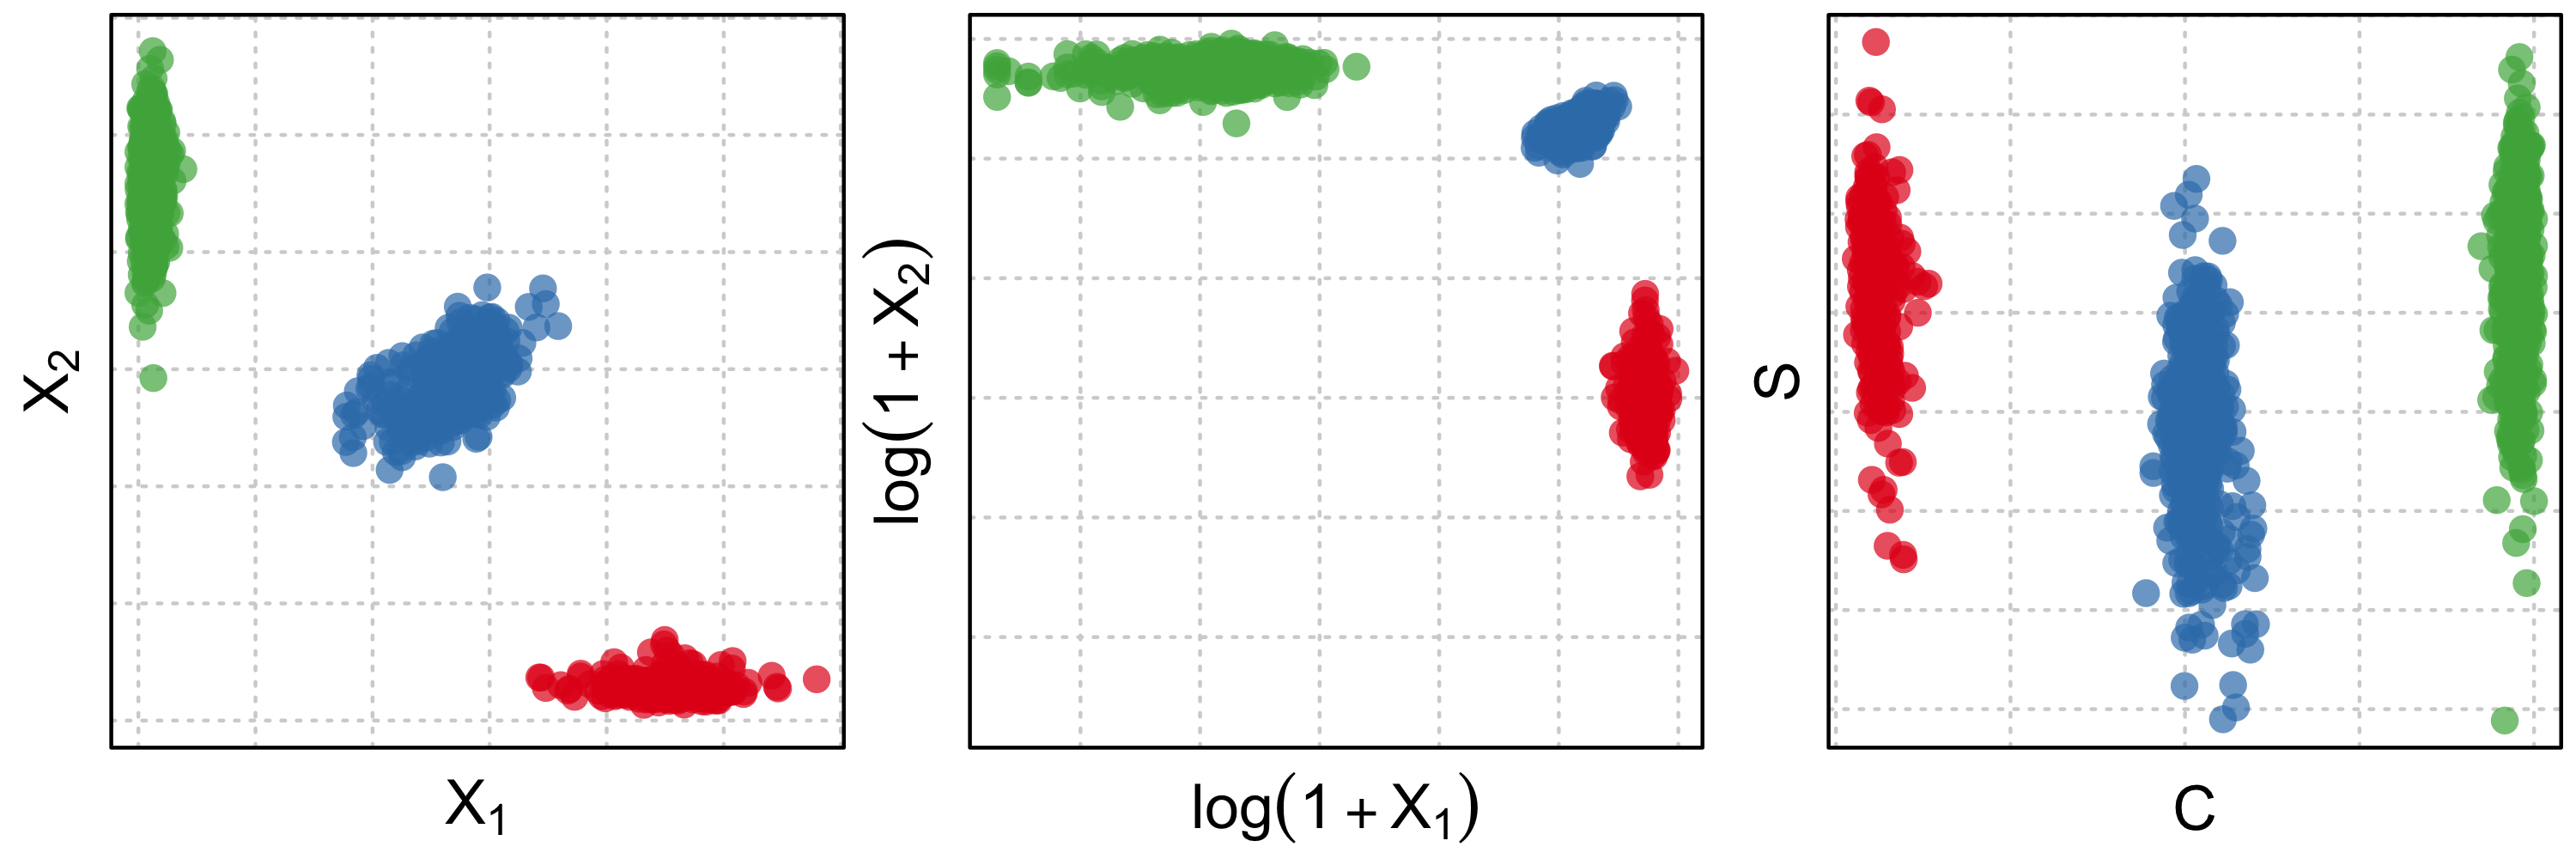
\includegraphics[width=\textwidth]{chap2figs/snpexample_1}
    \caption[Example microarray data from a typical high quality SNP]{Example microarray data from a typical high quality SNP from the Illumina Omni2.5S array assaying 1525 samples. The horizontal axis is the allelic intensity (or a transformation of it) for allele 1, the vertical axis is the intensity of allele 2.  Points are coloured by genotype called by Illumina's genotyping software.  Clusters are well separated and calling genotypes is not problematic. \textbf{Left:} The normalised values. \textbf{Centre:} The $\log$ transformed values which is the scale our algorithm works on. \textbf{Right:} The `strength' $S$ (vertical) and `contrast' $C$ (horizontal) transformations used by the Illuminus algorithm.}
\label{chap2:easysnp}
  \end{center} 
\end{figure}

\subsection{Genotype calling}
Assume we have microarray data on $N$ samples at a bi-allelic SNP as position $l$ and use $G_{il}$ to denote the unobserved genotype of the $i$th sample at this locus. The genotypes $G_{il}$ are the count of the number of non-reference alleles or a missing  value (NULL), that is $G_{il} \in \{0, 1 ,2, \NULL \}$. We use $\{I^1_{il}, I^2_{il}\}$ to denote the normalised bivariate signal intensities of the two alleles (1 and 2) at the SNP. In the following sections, we discard  $i$ or $l$ when we are only describing one particular SNP or individual respectively. The goal of genotype calling is to find the posterior probability of each genotype value given the microarray data, $P(G|I^1,I^2)$. Most methods achieve this via assuming some probability distribution $f_j(I^1,I^2;\theta_j)$ with parameters $\theta_j$ for the array data under genotype $j$, we can then calculate the posterior probability for each genotype via Bayes Rule:
$$P(G=j|I^1,I^2) = \frac{ P(G=j)\times f_j(I^1,I^2;\theta_j) } { \sum_{k=0}^3P(G=k)\times f_k(I^1,I^2;\theta_k) }$$
where $P(G=j)$ is the marginal probability of genotype $j$. We can then take $$\hat{G}=\argmax_jP(G=j|I^1,I^2)$$  as the hard genotype call for individual $i$. Additionally, if the posterior probability does not exceed some threshold we may flag it as missing. Alternatively (and more correctly), these posterior probabilities can be propagated through to other analyses such as phasing, imputation and association testing.

Genotype calling methods differ in three key ways; the choice of of probability distribution for $f_j(I^1,I^2;\theta_j)$, the parameter estimation routine for $\theta_j$ and choice of data transformation. We briefly describe the models and inference used by other methods the next section, we detail our own technique in section~\ref{chap2:chiamante}.

\subsection{Statistical distributions}\label{chap2:statdist}
We define several common statistical distributions that will be used throughout this chapter here.  

The bivariate Gaussian distribution:
$$\phi(X_i;\mu,\Sigma) = (2\pi)^{-d/2} |\Sigma|^{-1/2}\times exp\left(\half (X_i - \mu)^T\Sigma^{-1}(X_i-\mu)\right)$$
where $d=2$, $\mu$ and $\Sigma$ are the dimension, mean and covariance. 

The bivariate \st distribution:
$$s(X_i;\mu,\Sigma,\upsilon) = \frac{\Gamma(\frac{d+\upsilon}{2})}{\Gamma(\upsilon/2)(\upsilon\pi)^{d/2}}|\Sigma|^{-1/2} \times [1+\frac{1}{\upsilon}(X_i - \mu)^T \Sigma^{-1}(X_i - \mu)]^{-(d+\upsilon)/2}$$
where $\upsilon$ are the degrees of freedom.  The \st can be useful (as opposed to a Gaussian) if the data are over dispersed. We can also introduce a latent scale variable $u$ and represent the \st as a scaled mixture of normal distributions 
$$s(X_i;\mu,\Sigma,\upsilon) = \int_0^{\infty} \phi(X_i;\mu,\Sigma / u_i)Gam(u_i|\upsilon/2,\upsilon/2) du$$ where $Gam$ is the pdf of the Gamma distribution:
$$Gam(u_i|,\alpha,\beta) = \frac{\beta^\alpha}{\Gamma(\alpha)} u_i^{\alpha-1}e^{-\beta u_i}$$
This latent variable representation is useful as it allows proper estimation of the covariance matrix via the EM algorithm~\citep{peel2000robust}. This is important for the inference routine we describe in the section~\ref{chap2:inference}. 

%% The Beta distribution:

%% The Beta distribution is a useful prior for parameters that are constrained to be in the range $[0,1]$, for example the probability of success in a Binomial Distribution.


%% $$multinomial$$
%% $$Dirichlet$$

%% $$Inverse-Wishart$$

\section{Existing methods}
\subsection{Illumina's GenTrain2 Algorithm}
Illumina provides a proprietary algorithm (GenTrain) for genotype calling from its genotype microarrays as part of its Genome Studio software, the current version of the software is GenTrain2~\citep{gentrain2}.  In the typical use case, the end-user performs calling using a ``cluster file'' which contains pre-defined cluster centroids for each locus. These centroids were found using HapMap samples where genotypes at each locus are already known from previous assays.  Genotypes on new data are assigned according to which cluster an observation is nearest to. There is no formal description available of exactly what distance measure is used or how these initial clusters are estimated.  Nevertheless, as can be seen the results section the method produces highly accurate calls. We evaluate GenTrain2 calls that were created at the Broad Institute using the standard cluster file for the Omni2.5S chip.  These are available on the 1000 Genomes FTP site \footnote{\url{ftp://ftp.1000genomes.ebi.ac.uk/vol1/ftp/technical/working/20110527_bi_omni_1525_v2_genotypes/}}

\subsection{Illuminus}
Illuminus~\citep{Teo2007} fits a four component mixture of truncated bivariate \st distributions to the ``contrast'' and ``strength'' of the signal intensities at each locus.  Contrast and strength for a given SNP are defined respectively as,
$$C_{i} = \frac{I_i^1 - I_i^2}{I_i^1 + I_i^2}$$
$$S_{i} = \log(I_i^1 + I_i^2)$$
we plot the contrast and strength values for a SNP in Figure~\ref{chap2:easysnp}(right). Posterior probabilities for individual $i$ are found via,
$$P(G_i=j|C_i,S_i) \propto  \lambda_j~t_j(C_i,S_i;\mu_j,\Sigma_j,\upsilon_j)$$
where $\lambda_j$ are the frequencies of the genotypes for $j\in\{0,1,2\}$ constrained to be in Hardy-Weinberg Equilibrium, and $\lambda_{NULL}$ is the proportion of missing data. The density used for observations, $t_j$ is a truncated \st distribution with mean, variance and degrees of freedom equal to  $\mu_j$, $\Sigma_j$ and $\upsilon_j$ respectively;

$$t_0(C,S;\mu_0,\Sigma_0,\upsilon_0) = \frac{s(C,S;\mu_0,\Sigma_0,\upsilon_0)}{1-\int^{-1}_{-\infty} s(C,S;\mu_0,\Sigma_0,\upsilon_0) \textrm{d}C } $$

$$t_1(C,S;\mu_1,\Sigma_1,\upsilon_1) = \frac{s(C,S;\mu_1,\Sigma_1,\upsilon_1)}{\int^{1}_{-1} s(C,S;\mu_1,\Sigma_1,\upsilon_1) \textrm{d}C } $$

$$t_2(C,S;\mu_2,\Sigma_2,\upsilon_2) = \frac{s(C,S;\mu_2,\Sigma_2,\upsilon_2)}{1-\int_1^\infty s(C,S;\mu_2,\Sigma_2,\upsilon_2) \textrm{d}C } $$

where $s$ is the bivariate \st distribution. The truncation is used since $C$ is bounded in $[-1,1]$. Finally a flat bivariate Gaussian density with constant parameters is used for the NULL density with mean $\mu_{NULL}=(0.0,0.0)$ and covariance $\Sigma_{NULL}$ having zero covariance and diagonal equal to 100,000. The likelihood of the data is then
$$L (\lambda_k,\mu_k,\Sigma_k,\upsilon_k;C_{i},S_{i}) =  \prod_{i=1}^N  \sum_{k\in{\{0,1,2,NULL\}}} \lambda_k~t_k(C_{k},S_{k};\mu_k,\Sigma_k,\upsilon_k)$$ which we can be maximised with respect to the parameters via an Expectation-Maximisation (EM) algorithm.  This can be considered a ``population-based'' caller in that it optimises model parameters per SNP based on all individuals assayed at that SNP.

\subsection{GenoSNP}
GenoSNP~\citep{Giannoulatou2008} takes a novel approach in that it performs clustering `within-chip' to determine genotypes,  this means it is agnostic towards the number of individuals genotyped (it can accurately call one sample) and should be relatively unaffected by allele frequency.  It fits a four component student \st distribution to all the ($\log$ transformed) SNP intensities within each chip.  Let $X_{il}=\{\log(I^1_{il}+1),\log(I^2_{il}+1)\}$ be the log transformed intensities for marker $l$ and individual $i$, we drop $i$ henceforth.  Under the GenoSNP model, the posterior probability for genotype $j$ at locus $l$ (within a given individual) is proportional to

$$P(G_l=j|X_l) \propto \pi_j~s(X_j;\mu_j,\Sigma_j,\upsilon_j)$$ 

where $s$ is the bivariate student \st distribution for each genotype class with mean $\mu_j$, covariance $\Sigma_j$, degrees of freedom $\upsilon_j$ and $\pi_j$ is the frequency of genotypes occurring across all SNPs within an individual.  The likelihood for the GenoSNP model is 

$$L(\pi,\mu,\Sigma,\upsilon;X_l) = \prod_{l=1}^L \sum_{k\in\{0,1,2,NULL\}} \pi_k~s(X_l;\mu_k,\Sigma_k,\upsilon_k)$$

Note the likelihood is the product of all SNPs within an individual as opposed to all individuals within a SNP as was the case with Illuminus (and our method).  Inference is performed within a Bayesian framework with suitable priors on all parameters. Posterior distributions of the parameters are found via Variational-Bayes~\citep{archambeau2007robust}.  

\subsection{Genotype likelihoods generated from sequencing data}
Genetic variant detection from sequencing data is an ongoing topic of research in statistical genetics and bioinformatics~\citep{nielsen2011genotype}, but this is not an issue for our application since we know the physical locations and variants on the chip.  We simply require the genotype likelihoods (GLs) at these locations.  We used the pre-computed likelihoods from the 1000 Genomes project Phase I samples, sequenced at 4X.  These were calculated using BAM-specific binomial mixture modelling (BBMM) from the SNPTools software suite~\citep{wang2013integrative} which we briefly describe here.  

We denote sequence data from individual $i$ at locus $l$ as $Y_{il} = \{R_{il},A_{il} \}$, where $R_{il}$ and $A_{il}$ are the expected base depth (EBD) for the reference and alternate alleles respectively. The EBD is defined as
$$EBD_g = \sum_{\forall k=g} P(\textrm{Read k correct})\times P(\textrm{Alignment k correct})$$
here we sum over all reads reporting allele $g$. The probabilities correspond to the base quality and alignment quality.  This measure gives a read depth for each allele that is corrected for uncertainty. The corrected read depths are modelled as a mixture of binomial distributions \emph{within} each individual where $p_j$ is defined as the probability of a reference read given genotype $j$. If read and alignment quality was error free than $p_j = 1,0.5,0$ for $j=0,1,2$ respectively.

The genotype likelihood for a genotype $j$ at position $l$ is then
$$P(Y_{il}|G_{il}=j) = P(R_{il},A_{il}|G_{il}=j) = \binom{R_{il}+A_{il} }{A_{il}} p_j^{R_{il}} (1-p_j)^{A_{il}} $$
The parameter $p_j$ is estimated via EM.  The model we describe in the next section is ignorant towards the details of these calculations and simply takes the value of $P(Y_{il}|G_{il})$ as input.  Hence GLs calculated by other software/models such as SAMtools \citep{li2011improving} or GATK \citep{McKenna2010} could also be easily used.  We utilised pre-calculated GLs (using the SNPTools software) from 4X sequencing data on 1094 individuals from  1000 Genomes Phase I that were obtained from the 1000 Genomes FTP server in August 2011.

%\footnote{\url{http://ftp.1000genomes.ebi.ac.uk/vol1/ftp/technical/working/20110826_genotype_likelihoods/snps/}}.


\section{A joint model for microarray and sequence data}
\label{chap2:chiamante}
\subsection{Overview of the model}
%To develop our model we use the following notation. We assume that we have data on $N$ samples at a SNP and use $G_i$ to denote the unobserved genotype of the $i$th sample. The genotypes $G_i$ can take the values 0, 1 or 2 and count the number of non-reference alleles.
 We use $X_i  = \{\log(I_i^1+1), \log(I_i^2+1)\}$ to denote the microarray data for individual $i$ at a specific SNP within our framework (taking the logarithm was found to stabilise the variance and give better results). We assume that the sequence data for the $i$th sample at the SNP is available in the form of a Genotype Likelihood (GL), $P(Y_i|G_i=j)$ for $j\in\{0,1,2\}$. In situations where the ancestry of the samples are known it can be useful to allow for some model parameters to have population specific values, so we use $Q_i \in (1,\ldots,M)$ to denote a population label for the $i$th sample. In addition, we introduce latent variables, $Z_{X_i},Z_{Y_i} \in \{0,1\} $, that dictate the ``success'' or ``failure'' of the array or sequence data for the $i$th sample. That is, if $Z=0$ for a technology, we wish to utilise the information and if $Z=1$ the data can be considered spurious and discarded. Note that is straight forward to use this model when some (or all) individuals are not sequenced or not genotyped on the array, we simply set $P(Z_Y=1)=1$ or $P(Z_X=1)=1$ for those individuals as appropriate.

In general terms, the focus of our inference is the estimation of the unobserved genotypes, $G$, conditional upon the observed data, $(X,Y)$. Using a Bayesian framework we can achieve this goal by formulating a probabilistic model of the distribution of $G$ given $X$ and $Y$. Applying Bayes rule and making the assumption that the array and sequence data are conditionally independent given $G$ we have
\begin{equation}
P(G|X,Y) \propto P(X,Y|G)P(G) = P(Y|G)P(X|G)P(G). \nonumber
\end{equation}
We can then further partition on the ``success'' or ``failure'' of the array data
\begin{eqnarray*}
P(X | G) & = &\prod_{i=1}^N \left(P(X_i|G_i, Z_{X_i}=1)P(Z_{X_i}=1) + P(X_i|G_i,Z_{X_i}=0)P(Z_{X_i}=0)\right).\\
\end{eqnarray*}
We further assume that given a failure the array is independent of genotype so that this simplifies slightly to
\begin{eqnarray*}
P(X | G) & = &\prod_{i=1}^N \left(P(X_i|Z_{X_i}=1)P(Z_{X_i}=1) + P(X_i|G_i,Z_{X_i}=0)P(Z_{X_i}=0)\right).\\
\end{eqnarray*}
There are three parts of this model that we need to specify. When the array has ``failed'' we use a bivariate uniform distribution across the range of the allele intensities (across all SNPs) denoted as $h_X(x_i)$. This is equivalent to the NULL class used in other genotype calling approaches. We consider two possible distributions for when the array was successful, a bivariate Gaussian with mean and variance that depend upon genotype:
$$P(X_i| G_i=j,Z_{X_i}=0) = \phi(X_i;\mu_j,\Sigma_j)$$
where $\mu_j$ and $\Sigma_j$ are the  mean and covariance for genotype $G_i=j$. We also consider  a bivariate \st distribution:
$$P(X_i| G_i=j,Z_{X_i}=0) = s(X_i;\mu_j,\Sigma_j,\upsilon_j)$$
where $\upsilon$ are the degrees of freedom for genotype $G_i=j$. We found the \st with $\upsilon=5$ to produce more accurate results than the Gaussian (experiments detailed in Appendix A).

We specify the failure probability $P(Z_{X_i}=1) = 1 - P(Z_{X_i}=0) =\eta_X$ and estimate this parameter.

Similarly, for the sequence data we use 
\begin{eqnarray*}
P(Y | G) & = &\prod_{i=1}^N \left(P(Y_i|Z_{Y_i}=1)P(Z_{Y_i}=1) + P(Y_i|G_i,Z_{Y_i}=0)P(Z_{Y_i}=0)\right).\\
\end{eqnarray*}
Again, there are three parts to this model that we need to specify. The first one is the model of the sequence data when the sequencing has ``failed''. This is not an easy distribution to parameterise. A detailed model might include contextual information about the read quality, mapping quality and depth of coverage that could considerably complicate the modelling. We have found that setting $P(Y_i|Z_{Y_i}=1)$ equal to a small constant, $h_Y(y_i) = 0.01$ to work well,

The second part of the model is the term $P(Y_i|G_i=j,Z_{Y_i}=0)$ when the sequencing is a success. This is just the GL as described above. The three likelihoods were scaled to sum to one to ensure they were on a comparable scale to the ``failure'' likelihood, $h_Y(y_i)$. These specify the failure probability $P(Z_{Y_i}=1) = 1 - P(Z_{Y_i}=1) = \eta_Y$ which we estimate. Finally, we model the distribution of unobserved genotypes, $P(G)$, as $G_{i} \sim \textrm{Multinomial}(\lambda_{Q_i})$ where $\lambda_{Q_i}$ is a vector of genotype probabilities for population $Q_i \in \{1 \ldots  M\}$, where $Q_i$ indexes which of the $M$ populations individual $i$ comes from.  That is, we allow genotype frequencies to differ for different sub-populations in that data (such as the ethnicities present in 1000 Genomes data).

We use this model in a Bayesian Framework using maximum a posteriori probability (MAP) estimates of parameters.  A detailed description of the priors used is in the following sub-section and we give full details of there inference used in section~\ref{chap2:inference}.


\subsection{Priors}
\label{chap2:priors}
We place informative priors on the parameters of our model in the following way. We model the population genotype proportions $\lambda_m$ with a Dirichlet distribution parameterised to favour Hardy-Weinberg equilibrium with reference allele frequency, $\alpha_m$, and a variance parameter, $\delta$:
\begin{equation}
\lambda_m \sim \textrm{Dirichlet}(\alpha_m^2\delta,2\alpha_m(1-\alpha_m)\delta,(1-\alpha_m)^2\delta),  \qquad m \in (1,\ldots,M).
\end{equation}
This form of model was used in the CHIAMO and CNVCALL methods for calling genotypes and CNVs respectively~\citep{consortium2007,craddock2010genome, cardin2011bayesian}. We use $\delta=10$ based these models. The released version of our software uses a flat Beta prior for the reference allele frequency,$$\alpha_m \sim \textrm{Beta}(1,1),  \qquad m \in (1,\ldots,M),$$
Different choices of priors for $\alpha$ and $\lambda$ are evaluated in Appendix~\ref{chap2:results:exploratory:freq}. The different choices of prior do not appear to have a substantial effect on accuracy. 

Beta priors were also used for the sequence and array failure probabilities;
$$\eta_X \sim \textrm{Beta}(1,30),$$
$$\eta_Y \sim \textrm{Beta}(1,30).$$
We chose priors for sequence and array failure that reflect the fact that both these technologies ``fail'' relatively rarely.  However, some loci will be particularly difficult, hence our priors have a reasonable amount of mass over $0 < \eta < 0.2$.   


For the covariance matrix for each cluster, $\Sigma_j$, we us a standard conjugate Inverse-Wishart distribution,
\begin{eqnarray}
p(\Sigma_j) &=& \left(2^{\omega_jd/2}\pi^{d(d-1)/4} \prod^d_{k=1}\Gamma(\frac{\omega_j+1-k}{2})\right)^{-1} \nonumber\\
&\times& |\psi_j|^{\omega_j/2} |\Sigma_j|^{-(\omega_j+d+1)/2}\\\nonumber
& \times& \exp{(-\half \textrm{trace}(\psi_j\Sigma_j^{-1}))} \label{invWish}.
\end{eqnarray}
We undertook an exploratory analysis of the signal intensities to determine suitable values for the hyper-parameters in these prior distributions which is described section~\ref{chap2:results:exploratory}.


\subsubsection{Priors for $\mu$}
\label{chap2:method:muprior}
For the priors on cluster means, $\mu_j$, we  investigated three priors of increasing complexity.  Firstly the standard Normal-Inverse Wishart conjugate prior where the covariance of $\mu_j$ is dependent on $\Sigma_j$,
\begin{equation}\label{model1} \mu_j|\Sigma_j \sim \textrm{MVN}(\mu_{0,j},\Sigma_j/\kappa_{0,j}).\end{equation}
Secondly, a prior where the covariance of the cluster means, $\Sigma_{\mu_j}$, is not dependent on $\Sigma_j$,
\begin{equation}\label{model2} \mu_j \sim \textrm{MVN}(\mu_{0,j},\Sigma_{\mu_{j}}) \end{equation}
note this is not a conjugate prior.  Finally we tried a six variate Gaussian prior for all three means, that is, the centroids of each cluster are dependent on one another,
\begin{equation}\label{model3}\mu \sim \textrm{MVN}(\mu_0,\Sigma_{\mu})\end{equation}
 where $\mu_0$ is
\[ \left( \begin{array}{c}\mu_{0,0}\\\mu_{0,1}\\\mu_{0,2}\end{array}\right)\] 
again this is not a conjugate prior. 

The first prior is the standard conjugate prior and requires the covariance of $\mu_j$, $\Sigma_{\mu_j}$ to be linearly related to the covariance of the data $\Sigma_j$, exploratory analyses of the signal data suggested this was not the case.  The second, non-conjugate, prior removes this relationship.  The third prior enforces correlation between the genotype centroids which was suggested by our exploratory analysis, this may be particularly useful in the case of a cluster with very few observations, because we can borrow information from the location of the other cluster centroids.   We found the third prior to be the most accurate (albeit slightly) in some initial comparisons that are described in Appendix~\ref{chap2:results:centroid}.

%% For the priors of the cluster means we used a Gaussian prior for the joint distribution on cluster centroids that allows dependence between centroids. Our exploratory analysis found clear evidence of such correlation between cluster centroids (see section~\ref{chap2:results:exploratory}). This may be particularly useful in the case of a cluster with very few observations, because we can borrow information from the location of the other cluster centroids. The prior takes the form 
%% \begin{equation}\label{model3}\mu \sim \textrm{MVN}(\mu_0,\Sigma_{\mu}),
%% \end{equation}
%%  where $\mu_0$ is
%% \[ \left( \begin{array}{c}\mu_{0,0}\\\mu_{0,1}\\\mu_{0,2}\end{array}\right).\]
%% Here $\mu_{0,j}$ is the bivariate centroid when the genotype, $G=j$. We also explored two other choices of prior for $\mu$, one in which the centroids were not correlated and the standard conjugate Normal-Inverse-Wishart (described in~\ref{chap2:inference:ecm}, we found the prior described here to be slightly more accurate (see seciton~\ref{chap2:results:priors}).

\subsection{Inference}
\label{chap2:inference}
Ideally, we would like to obtain a full characterization of the posterior distribution of our model parameters and use this to obtain marginal estimates of the unobserved genotypes. This could be approximated using MCMC~\citep{gelman2004bayesian} or Variational Bayes~\citep{archambeau2007robust} but previous work (\cite{consortium2007} Supplementary) on similar problems suggests that a MAP (Maximum a posteriori) estimation approach, in which parameters that maximize the posterior distribution are sought, and then conditioned on to make inference is sufficient and stable. We use a Expectation Conditional-Maximisation (ECM) algorithm to maximize the posterior.  Through exploratory analysis (see section~\ref{chap2:results:exploratory}) we found a strong linear relationship between the maximum intensity  and the location of the centroids at a SNP. We exploit this relationship to find starting values for $\mu$ that provide robust convergence to the desired mode.  Priors and starting values for $\Sigma$ were also found via this analysis. 

\subsubsection{The Expectation Conditional Maximisation algorithm}
\label{chap2:inference:ecm}

The posterior probability of the parameters, $\theta$, for observations $i=1,\ldots,N$ in our model is,
\begin{eqnarray} p(\theta|x) = p(\theta)\prod^N_{i=1} \sum_{j=0}^2 &\lambda_{Q_i}\left(\eta_Xh_X(x_i) + (1-\eta_X) P(X_i| G_i = j,Z_{X_i}=0) \right)\nonumber\\
& \times\left(\eta_Yh_Y(y_i) + (1-\eta_Y)P(Y_i=y_i|G_i=j,Z_{Y_i}=0) \right)
\end{eqnarray}
where $p(\theta) = p(\eta_X)p(\eta_Y)\prod^M_{m=1}p(\alpha_m)p(\lambda_m|\alpha_m)\prod^2_{j=0}p(\mu_j,\Sigma_j)$ is our prior distribution of the parameters and $h$ are the failure densities of each data type. Finding parameter values that maximise the posterior is not possible analytically.  We utilise an Expectation Conditional-Maximisation (ECM) algorithm which is described in this section.

We introduce latent variables, $(g_{ij},z_i^Y,z_i^X)$, where $g_{ij}$ is one or zero according to whether observation $i$ belongs to $j^{th}$ class (genotype). $z_i^Y$ equals one if the $i^{th}$ sequence assay has failed and zero otherwise.  Similarly $z_i^X$ equals one if the $i^{th}$ sequence assay has failed and zero otherwise. We can then write the complete-data posterior probability as
\begin{eqnarray} p^C(\theta|x) = p(\theta)\prod^n_{i=1} \prod^2_{j=0} &\Big(\lambda_{Q_i} (\eta_Xh_X(x_i))^{z_i^X}((1-\eta_X)P(X_i| G_i = j,Z_{X_i}=0))^{1-z_i^X} \nonumber \\
&\times(\eta_Yh_Y(y_i))^{z_i^Y}((1-\eta_Y)P(Y=y_i|G=j))^{1-z^Y} \Big)^{g_{ij}}\end{eqnarray}

 We can iteratively compute the expectation of our latent variables, and hence the expected log posterior probability (the E-step), and then substitute these expectations into, and maximise, the complete data log posterior probability (the CM-step). We repeat these two steps until convergence. We can write the complete-data log posterior probability as,
\begin{equation} \log p^C(\theta|x) =  L_1(\eta_X) + L_2(\eta_Y) + L_3(\alpha,\lambda) + L_4(\upsilon) + L_6(\mu,\Sigma) + L_6 \nonumber \end{equation}
where
\begin{eqnarray}
L_1(\eta_X) &= &\log p(\eta_X) + \sum_{i=1}^nz_{X_i}\log\eta_X + \sum_{i=1}^n(1-z_{X_i})\log(1-\eta_X) \label{l1} \\
L_2(\eta_Y) & = & \log p(\eta_Y) + \sum_{i=1}^nz_{X_i}\log\eta_Y + \sum_{i=1}^n(1-z_{X_i})\log(1-\eta_Y) \\
L_3(\alpha,\lambda) &=& \sum_{m=1}^M\left[ \log p(\alpha_m) + \log p(\lambda_m|\alpha_m) +  \sum_{i=1}^n\sum_{j=0}^2 I(Q_i=m)g_{ij} \log\lambda_{m,j}\right] \label{l3} \\
L_4(\upsilon) & = & \sum_{i=1}^n(1-z_{X_i})\sum_{j=0}^2 g_{ij} \left\{-\log\Gamma(\half\upsilon) + \half\upsilon\log(\half\upsilon)+\half\upsilon(\log u_{ij} -u_{ij}) - \log u_{ij} \right\} \nonumber \\
L_5(\mu,\Sigma) &=& \sum_{j=0}^2\log p(\mu_j,\Sigma_j)\nonumber\\ 
&+& \sum_{i=1}^n (1-z_{X_i}) \sum_{j=0}^2 g_{ij} \left\{-\half d\log(\pi) - \half\log|\Sigma_j|  - \half u_{ij}(y_i - \mu_j)^T\Sigma_j^{-1}(y_i - \mu_j)\right\} \nonumber\\
&+& \sum_{i=1}^n z_{X_i} \sum_{j=0}^2 g_{ij} h_X(x_i) \label{l5} \\
L_6 & =  &\sum_{i=1}^n\sum_{j=0}^2 g_{ij} \{ (1-z_{Y_i})  P(Y=y_i|G=j) + z_{Y_i}h_Y(y_i) \} \\
&& ~~~~~~\times \{ (1-z_{X_i})  P(X=x_i|G=j) + z_{X_i}h_X(x_i) \}
\end{eqnarray}
We exploit the independence of these terms in the CM-step.  Recall that $u_{ij}$ is the weight in the infinite mixture formulation of the \st distribution described in section~\ref{chap2:statdist}.
\paragraph{Expectation step:}~\\
From~\ref{l1} to~\ref{l5} we can see that we need to calculate
$$E_{\theta^t}[G_{ij}|x_i,y_i] = \hat{g}_{ij}$$
$$E_{\theta^t}[Z_{X_i}|x_i,y_i] = \hat{z}_{X_i}$$
$$E_{\theta^t}[Z_{Y_i}|x_i,y_i] = \hat{z}_{Y_i}$$
$$E_{\theta^t}[u_{ij}|x_i,z_{X_i}=0] = \hat{u}_{ij}$$
$$E_{\theta^t}[\log u_{ij}|x_i,z_{X_ij}=0]$$
Given a set of parameters from the previous iteration, $\theta^\textrm{old}$, the first three expectations are straightforward to calculate,
$$\hat{g}^{\textrm{old}}_{ij} = \frac{\lambda^{\textrm{old}}_{Q_i,j} f_j^{\textrm{old}}(x_i,y_i)}{\sum^2_{k=0}\lambda^{\textrm{old}}_{Q_i,k} f_k^{\textrm{old}}(x_i,y_i)}$$
$$\hat{z}^{\textrm{old}}_{X_i} = \frac{\eta_X^{\textrm{old}}h_X(x_i)\sum_{j=0}^2\lambda^{\textrm{old}}_{Q_i,j}\left(\eta_Y^{\textrm{old}}h_Y(y_i) + (1-\eta_Y^{\textrm{old}}) P(Y=y_i|G=j) \right)}{\sum^2_{k=0}\lambda^{\textrm{old}}_{Q_i,k} f_k^{\textrm{old}}(x_i,y_i)}$$
$$\hat{z}^{\textrm{old}}_{Y_i} = \frac{\eta_Y^{\textrm{old}}h_Y(y_i)\sum_{j=0}^2\lambda^{\textrm{old}}_{Q_i,j}\left(\eta_X^{\textrm{old}}h_X(X_i) + (1-\eta_X^{\textrm{old}})s_j(x_i;\mu^{\textrm{old}}_j,\Sigma^{\textrm{old}}_j,\upsilon^{\textrm{old}})\right)}{\sum^2_{k=0}\lambda^{\textrm{old}}_{Q_i,k} f_k^{\textrm{old}}(x_i,y_i)}$$
where 
\begin{eqnarray}
f_j^{\textrm{old}}(x_i,y_i) = & \left( \eta_X^{\textrm{old}} h_X(x_i) + (1-\eta_X^{\textrm{old}}) 
s_j(x_i;\mu^{\textrm{old}}_j,\Sigma^{\textrm{old}}_j,\upsilon^{\textrm{old}}) \right) \nonumber\\
&\times \left(\eta_Y^{\textrm{old}}h_Y(y_i) + (1-\eta_Y^{\textrm{old}})P(Y=y_i|G=j)\right)\nonumber
\end{eqnarray}
It can be shown~\citep{peel2000robust} that 
$$\hat{u}^{\textrm{new}}_{ij}  = \frac{\upsilon^{\textrm{old}} + p }{\upsilon^{\textrm{old}} + (y_i - \mu_j^{\textrm{old}})^T\Sigma_j^{-1 \textrm{old}}(y_i - \mu_j^{\textrm{old}})}$$
and
$$E_{\theta^{\textrm{old}}}[\log u_{ij}|x_i,z_{X_i}=0] = \log\hat{u}^{\textrm{new}}_{ij} + \psi \left( \frac{\upsilon^{\textrm{old}}_j+p}{2} \right) - \log \left(\frac{\upsilon^{\textrm{old}}+p}{2} \right)$$
We can use these terms to calculate the expected complete-data log posterior probability.  
\paragraph{Conditional-maximisation step:}~\\
We cannot maximise the terms $L_3(\alpha,\lambda)$~(\ref{l3}) and $L_5(\mu,\Sigma)$~(\ref{l5}) independently for each parameter; $\alpha_m$ is dependent on $\lambda_m$ and vice versa.  Additionally $\mu$ may be dependent on $\sigma$ for some choices of priors. Hence we need to use the Expected Conditional Maximisation (ECM) algorithm, a variant of the EM algorithm.  The E-step is unchanged, while the M-step is replaced by a set of conditional maximisations.  Here we will choose $\alpha_m$ and $\mu$ to maximise $L_3(\alpha,\lambda)$ and $L_5(\mu,\Sigma)$ given the current estimates of $\lambda_m$ and $\sigma$ respectively.


We choose a new value for $\alpha_m$ by finding the value, $\alpha_m^{\textrm{new}}$, that maximises $L_3(\alpha,\lambda)$ with the current estimate of $\lambda_m$ substituted in (note we can drop the last term in the sum as it does not depend on $\alpha_m$),
$$\alpha_m^{\textrm{new}} = \argmax_{\alpha_m} \log p(\alpha_m) + \log p(\lambda_m\old|\alpha_m)$$
this does not have an analytical solution but the derivative can be calculated.  It is then straightforward to solve numerically (and quickly) by using Brent's Method~\citep{brent2002algorithms}.

Finding new values for $\lambda_m$ is a straightforward constrained optimisation problem which can be solved by using Lagrange multipliers, giving the update rules;
$$\lambda_{m,0}\new = \frac{(\alpha_m\new)^2 \delta -1 + \sum_{i=1}^n I(Q_i=m) \hat{g}\new_{i0}}{\delta((\alpha_m\new)^2 + 2\alpha_m\new(1-\alpha_m\new) + (1-\alpha_m\new)^2 - 3 + N_m}$$
$$\lambda_{m,1}\new = \frac{\alpha_m\new(1-\alpha_m\new) \delta -1 + \sum_{i=1}^n I(Q_i=m) \hat{g}\new_{i1}}{\delta((\alpha_m\new)^2 + 2\alpha_m\new(1-\alpha_m\new) + (1-\alpha_m\new)^2 - 3 + N_m}$$
$$\lambda_{m,2}\new = \frac{(1-\alpha_m\new)^2 \delta -1 + \sum_{i=1}^n I(Q_i=m) \hat{g}\new_{i2}}{\delta((\alpha_m\new)^2 + 2\alpha_m\new(1-\alpha_m\new) + (1-\alpha_m\new)^2 - 3 + N_m}$$
where $N_m = \sum_{i=1}^NI(Q_i=m)$

Similarly for $\eta_X$ and $\eta_Y$ we have
$$\eta_X\new = \frac{v^X-1+\sum_{i=1}^n\hat{z}\new_{X_i}}{v^X+w^X+N-2}$$
$$\eta_Y\new = \frac{v^Y-1+\sum_{i=1}^n\hat{z}\new_{Y_i}}{v^Y+w^Y+N-2}$$

The value of $\Sigma$ that maximises the expected log posterior probability can also be calculated analytically (conditional on the current value of $\mu$),
$$\Sigma_j\new = \frac{\nu_0 + \sum_{i=1}^n \hat{g}\new_{ij}(1-\hat{z}\new_{X_i})\hat{u}\new_{ij}(y_i-\mu\old_j)(y_i-\mu\old_j)^T}{\upsilon + d + 2 + \sum_{i=0}^n\hat{g}\new_{ij}(1-\hat{z}\new_i)}$$

Finally, the CM-step for $\mu_j$ varies depending which of the priors was used.  We considered three possible priors for the cluster means, $\mu_j$. 

\textbf{Model 1\label{model1}:} The standard Normal-Inverse Wishart conjugate prior where the covariance of $\mu_j$ is dependent on $\Sigma_j$
\begin{equation}\label{model1} \mu_j|\Sigma_j \sim \textrm{MVN}(\mu_{0,j},\Sigma_j/\kappa_{0,j}).\nonumber\end{equation}

\textbf{Model 2\label{model2}:} A prior where the covariance of the cluster means, $\Sigma_{\mu_j}$, is not dependent on $\Sigma_j$,
\begin{equation}\label{model2} \mu_j \sim \textrm{MVN}(\mu_{0,j},\Sigma_{\mu_{j}}) \nonumber\end{equation}

\textbf{Model 3\label{model3}:} A six variate Gaussian prior for all three means, that is, the centroids of each cluster are dependent on one another,
\begin{equation}\mu \sim \textrm{MVN}(\mu_0,\Sigma_{\mu})\nonumber\label{model3}\end{equation}
 where $\mu_0$ is
\[ \left( \begin{array}{c}\mu_{0,0}\\\mu_{0,1}\\\mu_{0,2}\end{array}\right)\] 

The last two choices are not conjugate priors, but the mode can be found which is sufficient for ECM.  The M-step for each possible prior is:

\textbf{Model 1\label{model1}:}
$$\mu_j\new = \frac{\mu_{0,j}\kappa_j + \sum_{i=1}^n\hat{g}\new_{ij}(1-\hat{z}\new_{X_i})\hat{u}\new_{ij}x_i}{\mu_{0,j}\kappa_j + \sum_{i=1}^n\hat{g}\new_{ij}(1-\hat{z}\new_{X_i})\hat{u}\new_{ij}}$$
\textbf{Model 2\label{model2}:} 
$$\mu_j^{\textrm{new}} = \left( \Sigma_{\mu_{0,j}}^{-1} + (\Sigma_j\new)^{-1}\sum_{i=1}^n\hat{g}\new_{ij}\hat{u}\new_{ij}\right)^{-1}(\Sigma_{\mu_{0,j}}^{-1}\mu_{0,j} + \sum_{i=1}^n\hat{g}\new_{ij}\hat{u}\new_{ij}(\Sigma_j\new)^{-1}x_i)$$
\textbf{Model 3\label{model3}:} 

For model 3 we exploit the property of the conditional distribution of a subset of variables from a multivariate normal distribution with mean $\mu_0$ and covariance $\Sigma_\mu$ also being multivariate normal.
If we partition $\mu_0$ and $\Sigma_\mu$ as follows
\[\mu_0 = \left[ \begin{array}{ccc}\mu_{0,j}\\\mu_{0,j'}\end{array}\right]\]

with sizes \[ \left[ \begin{array}{c} 2 \times 1\\4 \times 1 \end{array} \right] \] and

\[\Sigma_\mu = \left( \begin{array}{cc} \Sigma_j & \Sigma_{12}\\\Sigma_{21} & \Sigma_{22} \end{array}\right)\]

with sizes \[ \left[ \begin{array}{cc} 2 \times 2 & 2 \times 4\\4 \times 2 & 4 \times 4\end{array} \right] \]

Given $\mu_{j'}\new = a$, where $\mu_{j'}\new$ are the row vectors of $\mu\new$ not including $j$, the conditional distribution of $\mu_j$ is bivariate normal with mean
$$\bar{\mu}_{0,j} = \mu_{0,j} + \Sigma_{12}\Sigma^{-1}_{22}(a - \mu_{0,j'})$$
and covariance
$$\bar{\Sigma}_{\mu_{0,j}} = \Sigma_j - \Sigma_{12}\Sigma^{-1}_{22}\Sigma_{21}$$
given these values, we can apply the same update rule as used for Model 2.  When performing inference for the mixture of Gaussian distribution, we simply fix $u_{ij}=1$.

We stop the ECM algorithm when $\sum_{i=1}^N \sum_{j=0}^2 |\hat{g}_{ij}\new - \hat{g}_{ij}\old| < 10^{-3}$, that is, when the posterior probabilities of the genotypes have stabilised.

\section{Implementational details}
\label{chap2:results}
\subsection{Exploratory analyses to determine prior and starting values}
\label{exploratory}
\label{chap2:results:exploratory}
We have described how to fit our model, but have not given specific values for the priors distributions on $\mu$ and $\Sigma$, nor have we described how starting values are chosen.  We undertook an exploratory analysis of high quality SNPs to resolve these issues. We took the signal intensities from 1000 SNPs with MAF $>$ 0.1 and $<1\%$ missingness (calculated from GenTrain2 genotypes), that is, SNPs with sufficient observations in each genotype cluster to easily fit a mixture distribution.  We then fitted a four component bivariate Gaussian mixture distribution in a frequentist framework using EM. The means and covariances at each of these easy SNPs were used to determine sensible prior values.  We also found a strong relationship between the means of the centroids and the maximum allelic intensity, this was used to choose starting values for SNPs `on the fly'.
\subsubsection{Prior values for centroids and covariance matrices}
The cluster means of the three genotype clusters are plotted in Figure~\ref{priors1} (left panel) and show clear clustering of the centroids for each genotype class. Since each SNP produces six parameter estimates (estimates of the mean for the intensities of alleles 1 and 2 of each genotype cluster centroid) we can examine the correlation between these values. Figure~\ref{mupairs} shows a plot of all pairs of parameter estimates and illustrates that clear correlations exist both between the allele 1 and 2 mean estimates \emph{within} each genotype class and \emph{between} genotype classes. This suggested the use of a joint prior for the cluster centroids (Model 3 in section~\ref{chap2:method:muprior}). We estimated $\mu_0$ and $\Sigma_{\mu}$ using the standard maximum likelihood estimators. To estimate the parameters of the inverse-Wishart prior on the distribution of the within cluster errors (equation~\ref{invWish}), we used the estimated covariance matrices from the 1000 SNPs applied the downhill simplex algorithm~\citep{nelder1965downhill} to maximise the log-likelihood of this sample, using suitable transforms to keep $\psi_j$ positive definite and $\omega_j$ positive.  It is difficult to visualise observations from the inverse-Wishart distribution, but we simulated some covariance matrices from our estimated distributed and overlaid the contours of the results distribution on some real signal data (Figure~\ref{priors1} bottom) and the results appear reasonable.

Given we estimated our priors using data from ``easy'' SNPs, we were interested to see if they were reasonably consistent with our MAP estimates for all loci.  We plot MAP estimates using the full Bayesian model with sequence data of centroid for all loci on chromosome 20 in Figure~\ref{priors1} (top right) and shade the points according to allele frequency.  The priors and the posteriors appear reasonably consistent with one another and the distributions of centroids do not vary greatly with MAF.

\begin{figure}
  \begin{center} 
    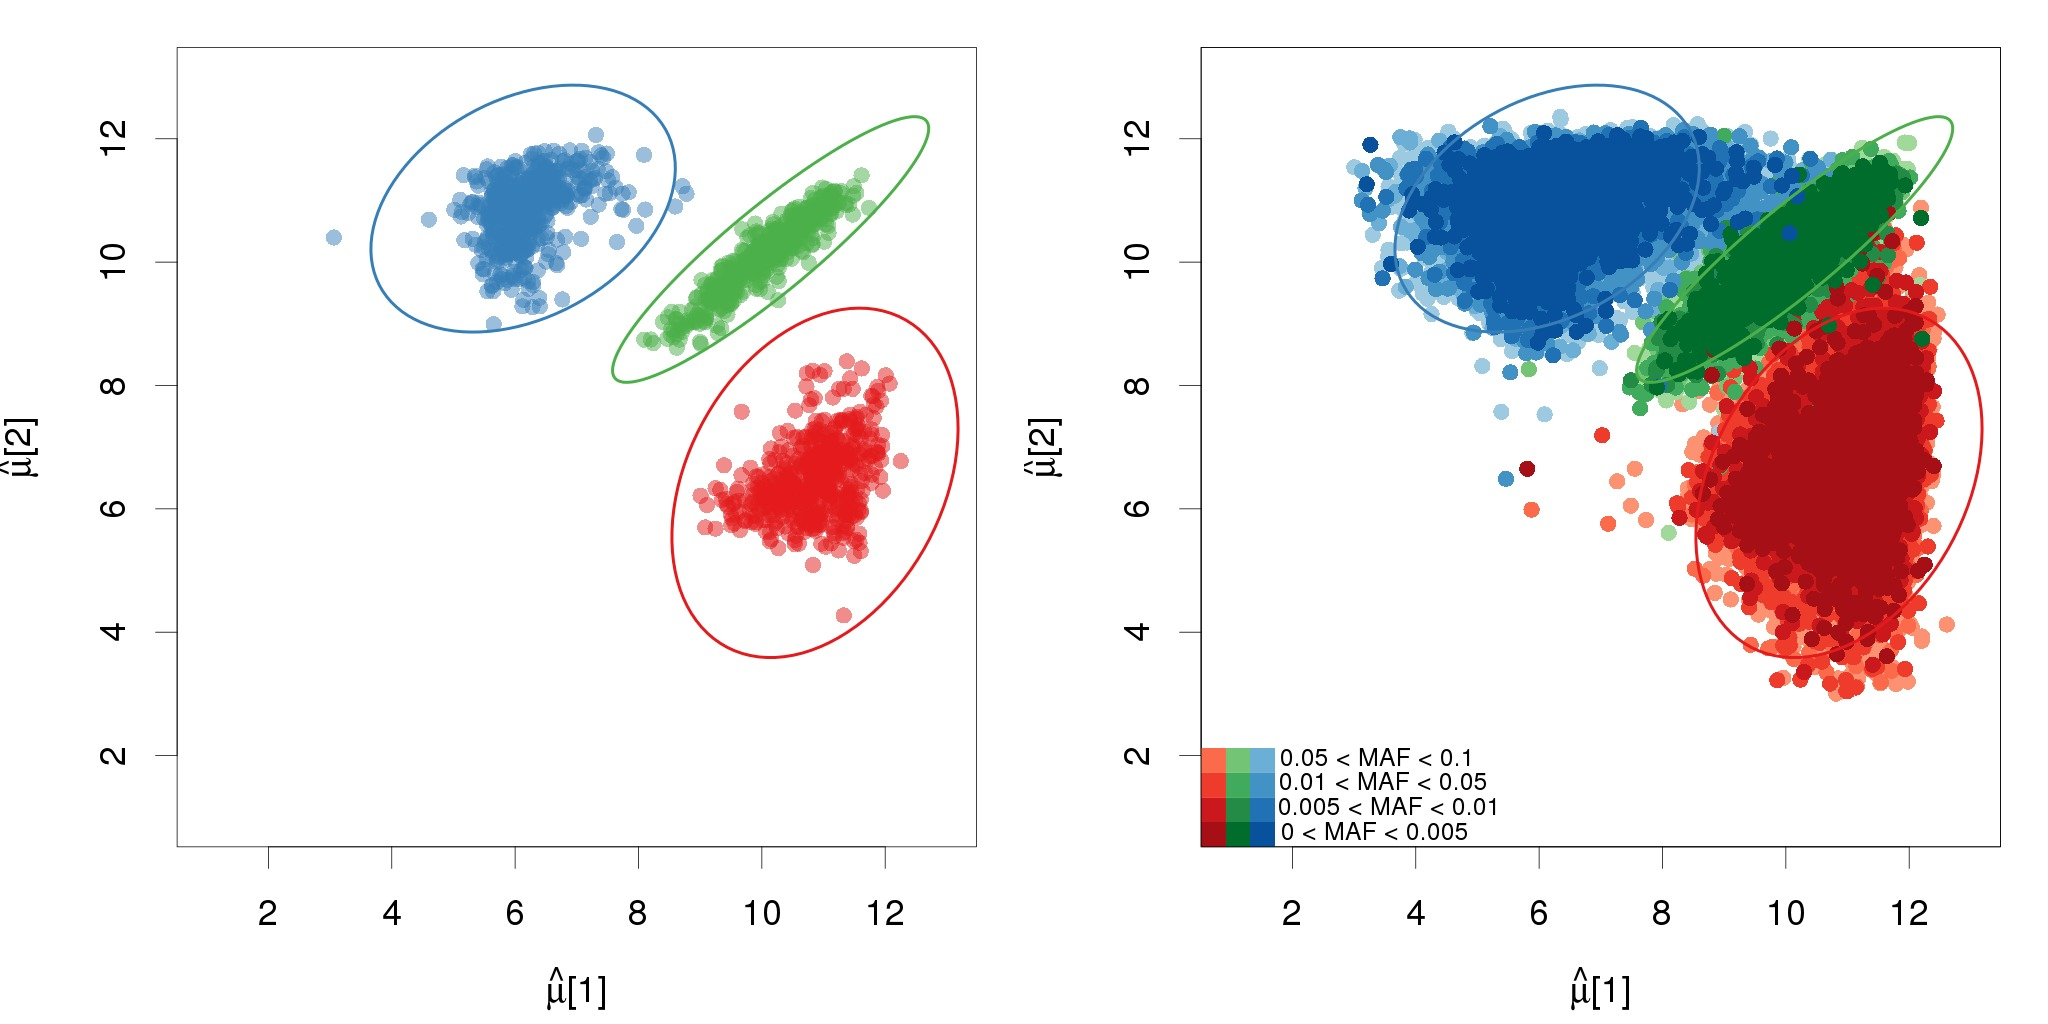
\includegraphics[width=\textwidth]{chap2figs/SupFig5}\\
    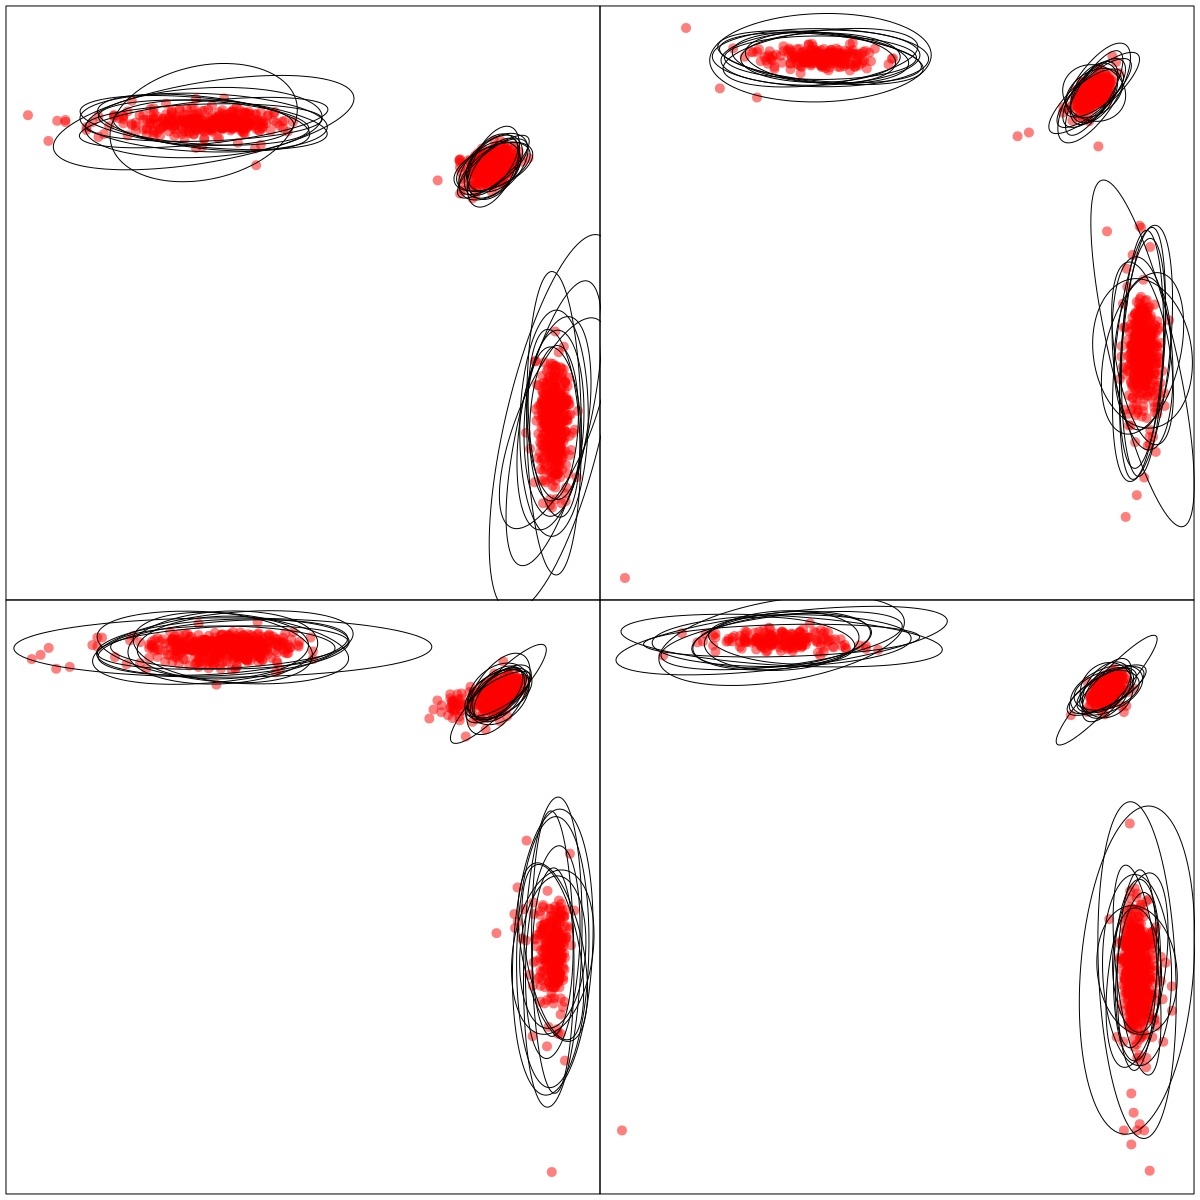
\includegraphics[width=.8\textwidth]{chap2figs/SupFig6}
    \caption[Comparison of priors and MAP estimates for our genotype calling model]{\textbf{Top left:} The estimated centroids for 1000 SNPs, the contour is the 99.9\% confidence interval of the centroid prior. \textbf{Top right:} MAP estimates of centroids (using array and sequence data) for 55126 SNPs on chromosome 20 with points shaded according to MAF.  There does not appear to be any strong relation between allele frequency and centroid location. \textbf{Bottom:} Signal intensities from four SNPs with 99.9\% confidence contours of ten simulated covariance matrices from the prior.\label{priors1}}
  \end{center} 
\end{figure}

\begin{figure}
\begin{center} 
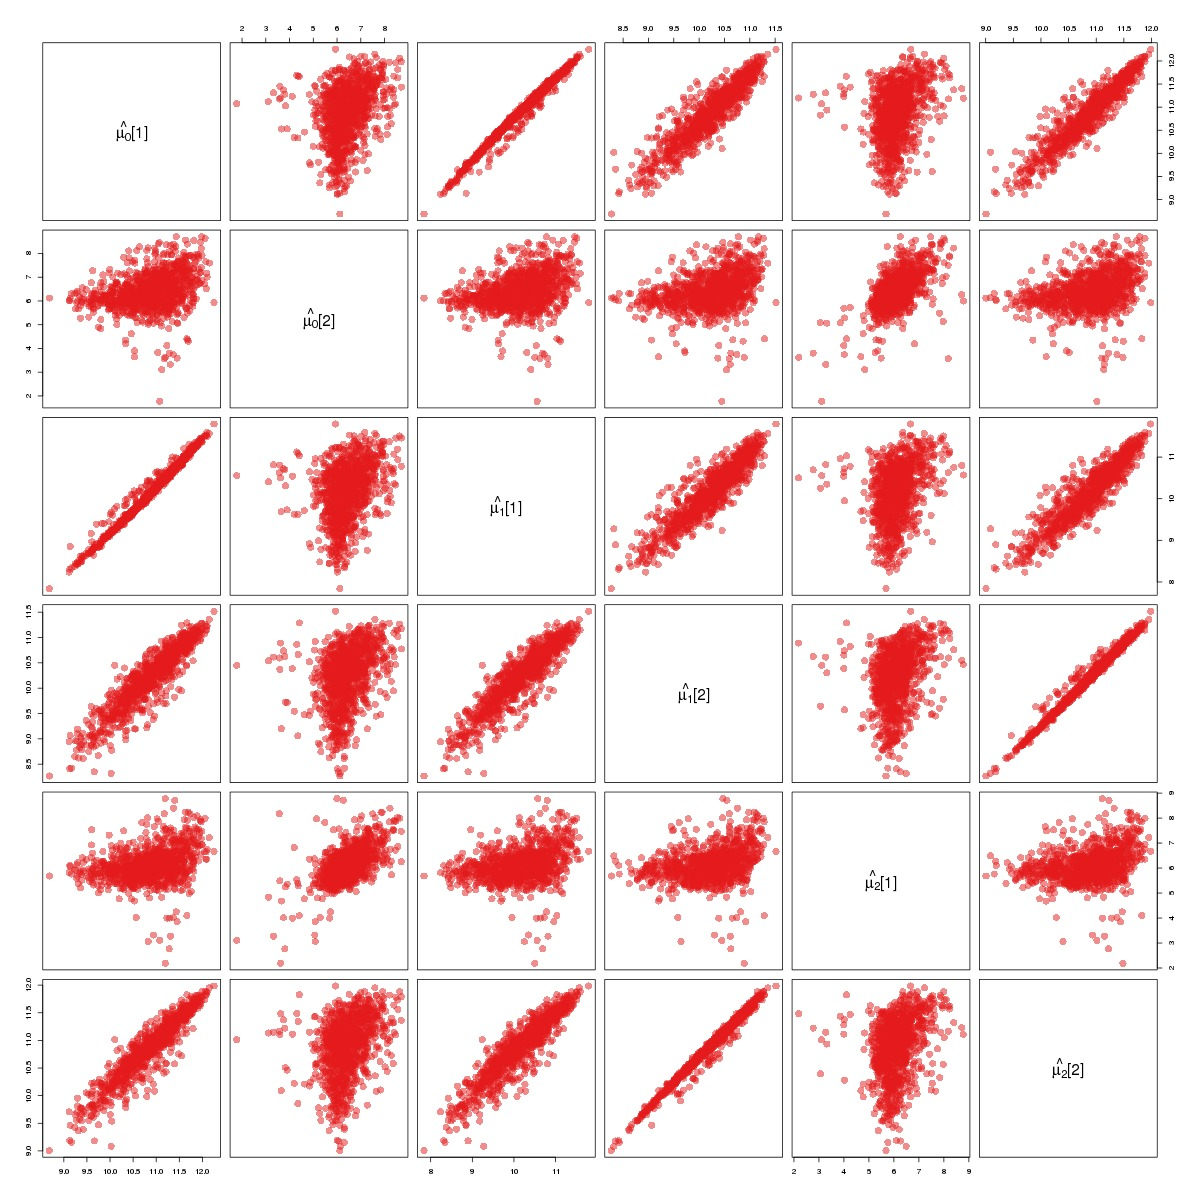
\includegraphics[width=\textwidth]{chap2figs/SupFig7}
\caption[Correlations between cluster centroids]{A pairs plot of the values for each mean estimate from the 1000 training SNPs.  We can see there is a strong correlation between the locations of the cluster centroids which may be exploited when choosing our priors.  The covariance of this data was used for the second (one off diagonal) and third priors.\label{mupairs}}
\end{center} 
\end{figure}
\clearpage
\subsubsection{Starting values}
Sensible starting values are crucial for fast convergence of our algorithm as well as converging to the desired mode of the posterior distribution.  Whilst the majority of SNPs have very good separation between genotype clusters, the location of the centroids of these clusters vary greatly between SNPs. Figure~\ref{centroid_eg} gives an example of two loci with high quality data but very different centroid locations. This means that using a constant set of starting values for parameters can be problematic. We undertook exploratory analyses on the centroid means estimated from easy SNPs to see if sensible starting values could be found from some simple sample statistic (for example, maximum allelic signal intensity).

We regressed each of the values in the three bivariate centroid means against the 95\% quantile of the allele intensity magnitude $\left( \sqrt{(X^1)^2+(X^2)^2} \right)$ for each allele, giving us six regressions in total.  We can see there is a strong relationship between  magnitude quantile and the centroids of the clusters (Figures~\ref{reg1}).  We exploit this relationship to select starting values that allow quick convergence of our ECM algorithm to the desired mode by calculating the quantile at each SNP and setting the centroid starting values according to the least squares estimates show in Figure~\ref{reg1}.

\begin{SCfigure}[1][h]
\centering
    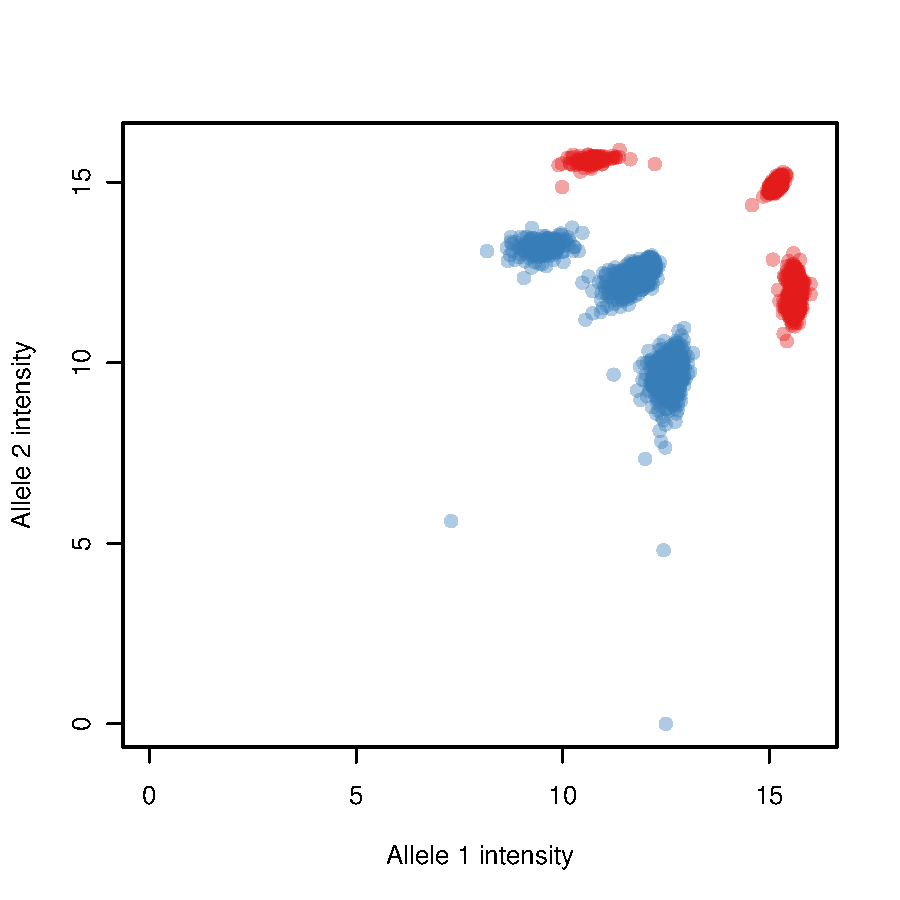
\includegraphics[width=.5\textwidth]{chap2figs/SupFig1}
    \caption[Signal intensities from two SNPs with very different cluster locations]{Signal intensities from two separate SNPs, whilst discrimination is good, the locations of the cluster centroids vary greatly.  This makes it difficult to rely on constant starting values between SNPs.  \label{centroid_eg}}
\end{SCfigure}
\clearpage

\begin{figure}
 \begin{center}  
               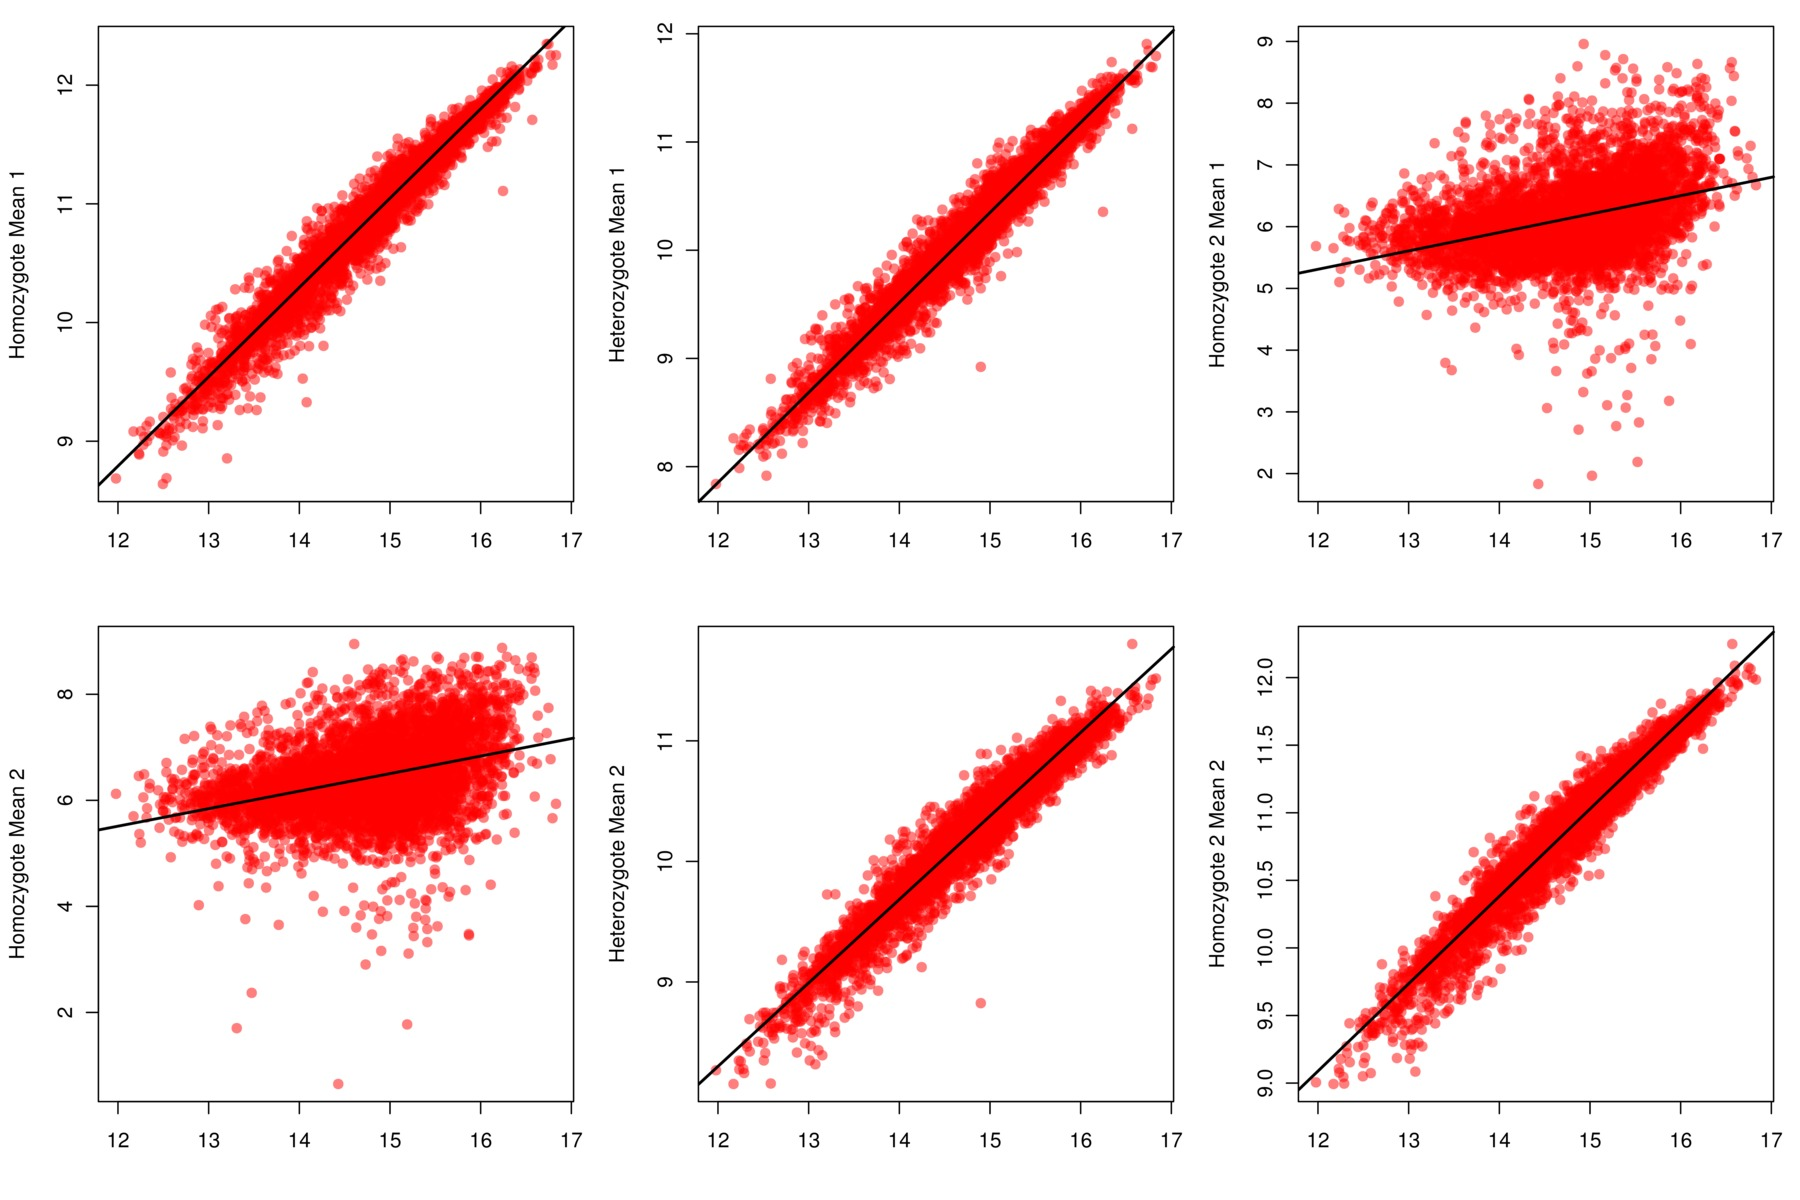
\includegraphics[width=\textwidth]{chap2figs/SupFig8}
\caption[Comparison between cluster centroids and maximum allele intensities]{The scalar elements of each centroid regressed against the 95\% quantile of the allele intensity magnitude. There is a strong relationship between this value and the location of the means.\label{reg1}}
\end{center} 
\end{figure}
\clearpage
\subsection{Posterior probabilities in output}
The Illuminus and GenoSNP methods both output posterior probabilities $P(G=j|\textrm{Data})$ for genotypes $G \in (0,1,2,\textrm{NULL})$. Observations are assigned to the ``NULL'' class by these methods when the array data does not appear to come from one of the three genotype clusters.  Our method uses two latent variables to indicate failed sequence and array assays for each genotype which allows us to call genotypes when at most one of the assays fails. This means when the failure parameters are high, causing $P(\textrm{Data}|G=j)$ to be flat, the posterior probability will tend towards to population frequency of the genotypes since we have no explicit ``NULL'' class.  This is reasonable behaviour but means our method is not directly comparable to other callers.  This is issue is easily circumvented by calculating a slightly different probability.

We calculate the posterior probability of a ``NULL'' genotype as the posterior probability that both assays have failed
\begin{eqnarray*}
P(G_i = \textrm{NULL}|X_i,Y_i)  &=& P(Z_i^X=1 \cap Z_i^Y=1|X_i,Y_i).
\end{eqnarray*}
We call genotypes when at least one of the assays has succeeded using
\begin{eqnarray*}
 P(G_i = j|X_i,Y_i,Z_i^X=0 \cup Z_i^Y=0) &\propto& P(G=j) P(X_i,Y_i|Z_i^X=0 \cup Z_i^Y=0) \qquad j \in {0,1,2}.
\end{eqnarray*}

We use these probability values for methods evaluation in section~\ref{chap2:results:comparison} as it makes Illuminus, GenoSNP and Chiamante directly comparable. GenTrain2 does not provide a posterior probability per genotype although does flag genotypes as missing when the array data is atypical, we just take the hard calls from GenTrain2.


\section{Data sets}
\label{chap2:data}
We evaluated our method in several ways using real data from Phase 1 of the 1000 Genomes Project. The data consist of a total of 1,525 samples from 15 populations. There are 1,525 samples with allele intensity data from the Illumina Omni2.5S genotyping chip. A subset of 1094 of these samples also have low-coverage (4X) sequencing data available, summarised in the form of genotype likelihoods.   In addition, we used genotype data on 1261 samples from an Affymetrix Axiom genotyping chip to assess the performance of methods, by taking the Affymetrix genotypes to constitute the true genotypes. There are 828 samples typed on both Omni2.5S and Axiom chips. There are 623 samples with data from all three technologies. This data is summarised in Figure~\ref{venn} and full details of the samples are in supplementary table~\ref{chap2:sampleinfo}.

\begin{SCfigure}[1][h]
\centering
    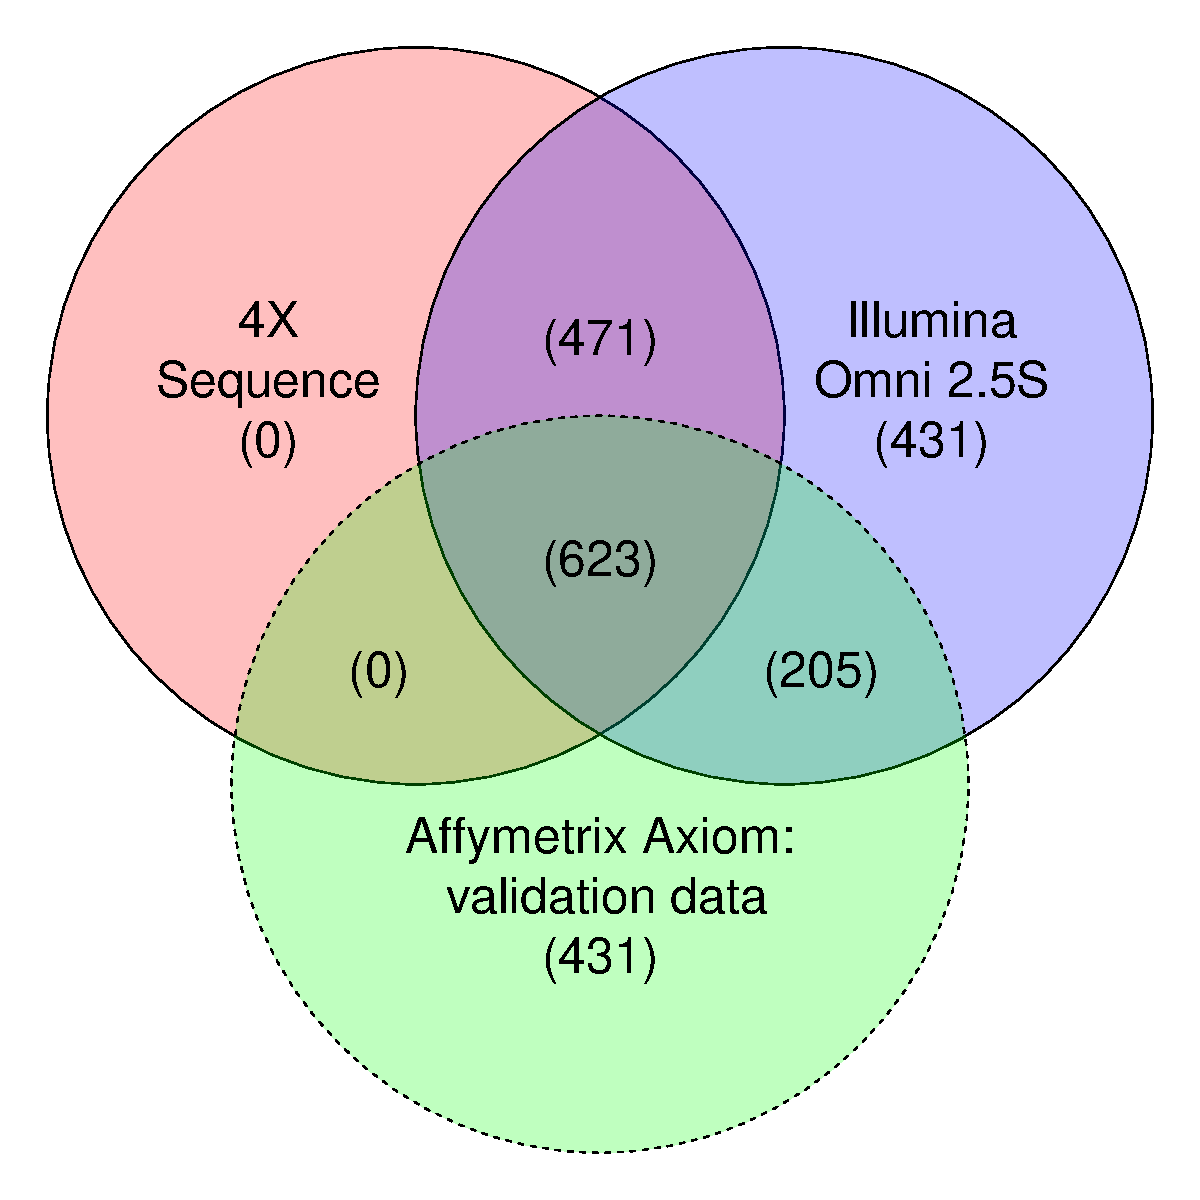
\includegraphics[width=.4\textwidth]{chap2figs/venn}
    \caption[The available samples assayed on each genotyping technology]{Venn diagram summarising the available samples assayed on each technology.  We developed models and made genotype calls for the sequence and Illumina Omni 2.5S data and used genotypes from the Affymetrix Axiom chip as validation data.  \label{venn} }
\end{SCfigure}


\subsection{Evaluating accuracy}
The easiest way to compare methods is to force each method to make a call of each genotype and then calculate the concordance with the calls made on the Axiom chip. In a real study it is usual to apply filters that exclude individual genotypes or whole SNPs that seem to have spurious genotype calls and then measure concordance on the genotypes that have passed the filters. We use the notation $\hat{G}_{il}$ to denote the genotype call made in the $i$th individual at the $l$th SNP. By default this genotype call (either 0, 1, 2 or NULL) will be the one which has the highest posterior probability. The result of applying a filter will be to set some of these genotype calls to NULL.

Once the filter has been applied we can calculate the genotype call rate (GCR), which is the percentage of all non-NULL genotypes, defined as 
\begin{equation}
\textrm{GCR} = 100 \times \frac{\sum_{i=1}^N \sum_{l=1}^L I(\hat{G}_{il}\neq \textrm{NULL})}{N \times L}
\end{equation}
and the percentage concordance of the non-NULL genotype calls with the non-NULL Affymetrix Axiom genotypes, defined as 

\begin{equation}
\textrm{Concordance} = 100 \times \frac{ \sum_{i=1}^N \sum_{j=0}^2 \sum_{l=1}^L I(G_{il}^{\textrm{Axiom}} = j) I(\hat{G}_{il}=j)}{\sum_{i=1}^N \sum_{l=1}^L I(G_{il}^{\textrm{Axiom}}\neq \textrm{NULL}) I(\hat{G}_{il}\neq \textrm{NULL}) } \label{concordance}
\end{equation}

We considered three standard filters. The first filter removes all genotypes with a posterior probability (PP) below 0.9. The second filter removes whole SNPs that show departures from Hardy-Weinberg Equilibrium (HWE). Since the data we use for the comparisons consists of multiple populations we calculate a p-value for a test of HWE in each of $M$ populations separately and then consider the minimum p-value across populations which has a Beta(1, $M$) distribution under the null of independent populations all in HWE. We exclude SNPs for which the resulting p-value is less that $10^{-7}$. The third filter removes whole SNPs where the SNP call rate (SCR) is below 0.9. SNP call rate is defined as the percentage of genotypes that were not NULL.  When the posterior probability filter is applied in conjunction with the SCR filter, a NULL genotype is defined as one having a posterior probability below 0.9. We consider all combinations of these filters which allows us to investigate the properties of our method compared to GenoSNP, Illuminus and GenTrain2. Note that GenTrain2 does not produce posterior probabilities so we just report the call rate and accuracy according to its hard genotype calls.


\clearpage
\section{Evaluating different genotype calling algorithms}
\label{chap2:results:comparison}

\subsection{Data sets with only array data on all samples} 

We compared our method to a range of other approaches  in the standard genotype calling scenario where only array data is available on the study samples. We called genotypes for the 1,525 1000 Genomes project individuals using only the Omni2.5S signal intensities (no sequence data) and assessed performance using the 828 individuals who were also assayed on the Affymetrix Axiom chip.  Table~\ref{chap2:arrayconc} shows the results of our method compared to Illuminus, GenoSNP and GenCall on the unfiltered data as well as all combinations of these filters. The table shows the overall call genotype call rate (GCR), the SNP call rate (SCR) and the concordance (Conc) for each method. Without any filters applied all the methods seem perform broadly the same with genotype call rates roughly between 99.72\% and 99.93\% and concordance between 99.63\% and 99.71\%. A more realistic comparison is how the methods perform after applying different QC filters.

The different filters have different effects on the different methods. Possibly the most striking result is the filter on HWE which removes a relatively large number of SNPs for GenoSNP and Illuminus (but not Chiamante or GenTrain2). This filter removes 0.33\% and 0.5\% of SNPs for GenoSNP and Illuminus respectively without very much effect on concordance. Figure~\ref{seq1,525qq} highlights this feature of the methods further by showing the quantile-quantile plots of the HWE p-values for each method. The figure shows that substantially more SNPs have extreme HWE p-values when using GenoSNP and Illuminus compared to using Chiamante or GenTrain2. In practice, this translates to $>5000$ extra SNPs that would pass QC and hence be available for downstream analyses when using Chiamante or GenTrain2 versus Illuminus or GenoSNP.

When all the filters are combined we find that all the methods have a Concordance of between 99.71\%-99.73\% but the methods have differing GCR and SCR. Chiamante increases GCR over GenoSNP and Illuminus by 1\% and 0.1\% respectively. It also increases SCR over GenoSNP and Illuminus by 0.9\% and 0.2\% respectively. Comparing all the methods when just the SCR and HWE filters are applied the best two methods are Chiamante and GenTrain2. The concordance between these two methods is roughly the same, Chiamante has a better GCR by 0.03\% and GenTrain2 has a better SCR by 0.07\%. 

We also examined the effect of each individual filter on the different methods by varying the filter thresholds. Figure~\ref{arrayfig} shows the percentage of missing data versus concordance for each of the methods as the filters thresholds are varied. This figure highlights how GenTrain2 seems remarkably robust to the various filters and that the PP and HWE filters have a much bigger effect on the performance of Illuminus and GenoSNP.  
%\begin{landscape}
\vspace{20pt}
\begin{table}[h]
\begin{center}
 \resizebox{\textwidth}{!}{
\begin{tabular}{|l|rrr|rrr|rrr|rrr|}
  \hline
  & \multicolumn{3}{c|}{Chiamante}& \multicolumn{3}{c|}{GenoSNP}& \multicolumn{3}{c|}{Illuminus} &\multicolumn{3}{c|}{GenTrain2}  \\
  \hline
 Filter & GCR & SCR & Conc & GCR & SCR & Conc& GCR & SCR & Conc& GCR & SCR & Conc\\
  \hline
  None & 99.824 & 100.000 & 99.696 & 99.802 & 100.000 & 99.632 & 99.930 & 100.000 & 99.670 & 99.720 & 100.000 & 99.707 \\ 
  \hline
  SCR & 99.646 & 99.765 & 99.698 & 99.516 & 99.634 & 99.666 & 99.877 & 99.927 & 99.678 & 99.605 & 99.822 & 99.710 \\ 
  HWE & 99.766 & 99.941 & 99.708 & 99.509 & 99.669 & 99.683 & 99.436 & 99.496 & 99.701 & 99.677 & 99.955 & 99.712 \\ 
  PP & 99.744 & 100.000 & 99.715 & 99.470 & 100.000 & 99.683 & 99.896 & 100.000 & 99.679 &  - & - & - \\
  \hline
  SCR+HWE & 99.590 & 99.710 & 99.709 & 99.345 & 99.457 & 99.693 & 99.406 & 99.455 & 99.706 & 99.568 & 99.783 & 99.714 \\ 
  PP+SCR & 99.520 & 99.694 & 99.722 & 98.605 & 98.857 & 99.710 & 99.826 & 99.905 & 99.692 &  - & - & - \\
  PP+HWE & 99.696 & 99.940 & 99.722 & 99.095 & 99.508 & 99.715 & 99.413 & 99.501 & 99.708 &  - & - & - \\
  \hline
  All & 99.486 & 99.659 & 99.726 & 98.508 & 98.756 & 99.721 & 99.381 & 99.456 & 99.713 & - & - & - \\
  \hline
\end{tabular}
}
 \caption[Genotype calling  performance and effect of different QC filters]{Genotype call rate (GCR), SNP call rate (SCR) and concordance (Conc) in \% for different genotype calling methods applied to 1,525 samples assayed on the Omni2.5S chip and validated against a subset of 828 of these samples also assayed on the Affymetrix platform. Each row corresponds to a different combination of filters applied to the data. The PP filter removes all genotypes with a posterior probability below 0.9.  The HWE filter removes whole SNPs that show departures from HWE. The SCR  filter removes whole SNPs where the call rate is below 0.9. Call rate is defined at the percentage of genotypes that were not ``NULL'' }
\label{chap2:arrayconc}
\end{center}
\end{table}
%\end{landscape}

\begin{SCfigure}
\centering
    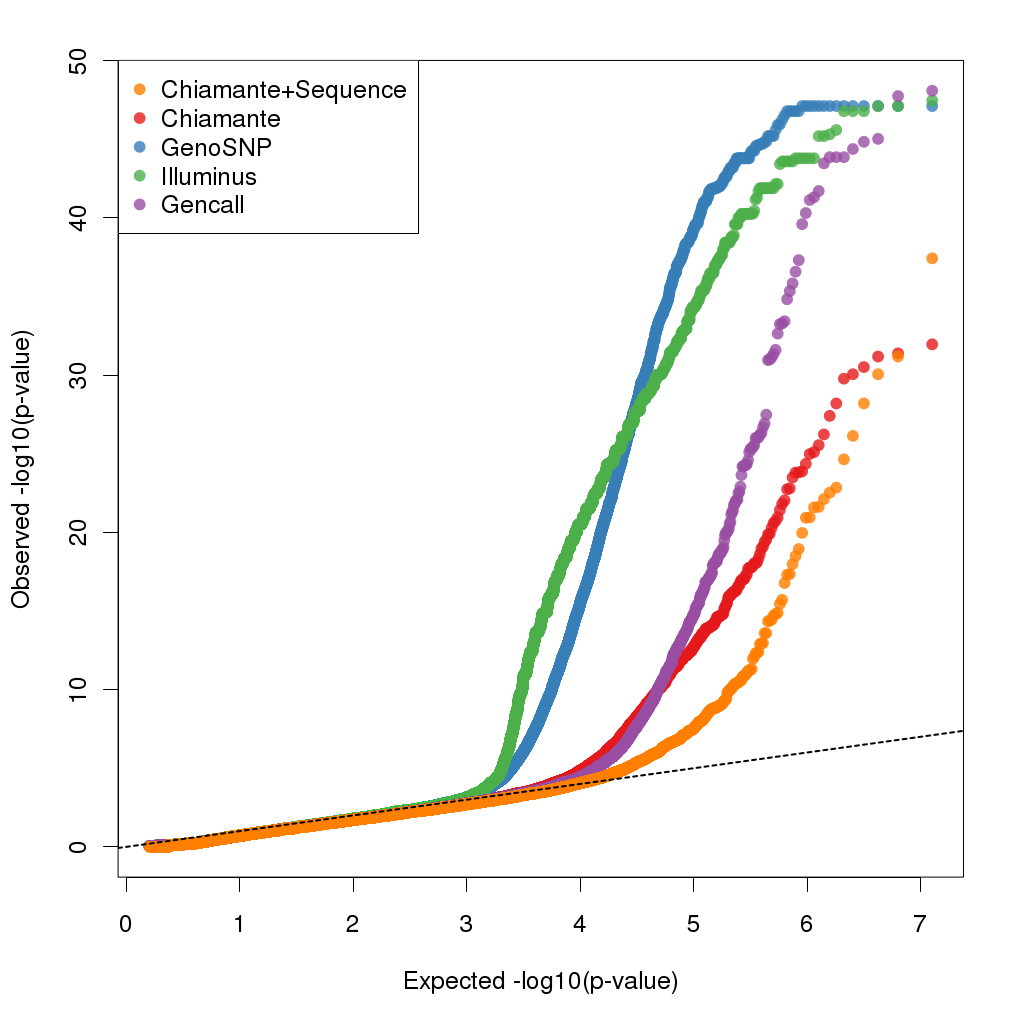
\includegraphics[width=.5\textwidth]{chap2figs/Fig3}
    \caption[Q-Q plots of HWE p-values for different genotype calling methods]{Q-Q plots of observed versus expected HWE p-values for different methods. Calls were made using each algorithm applied to Omni2.5S data from 1,525 individuals (17 different populations). The p-value is calculated at each locus by considering the minimum of the p-value for a test of HWE in each of $17$ populations separately which has a Beta(1, 17) distribution under the null of independent populations all in HWE.
      \label{seq1,525qq}}
\end{SCfigure}

\begin{figure}
  \begin{center} 
    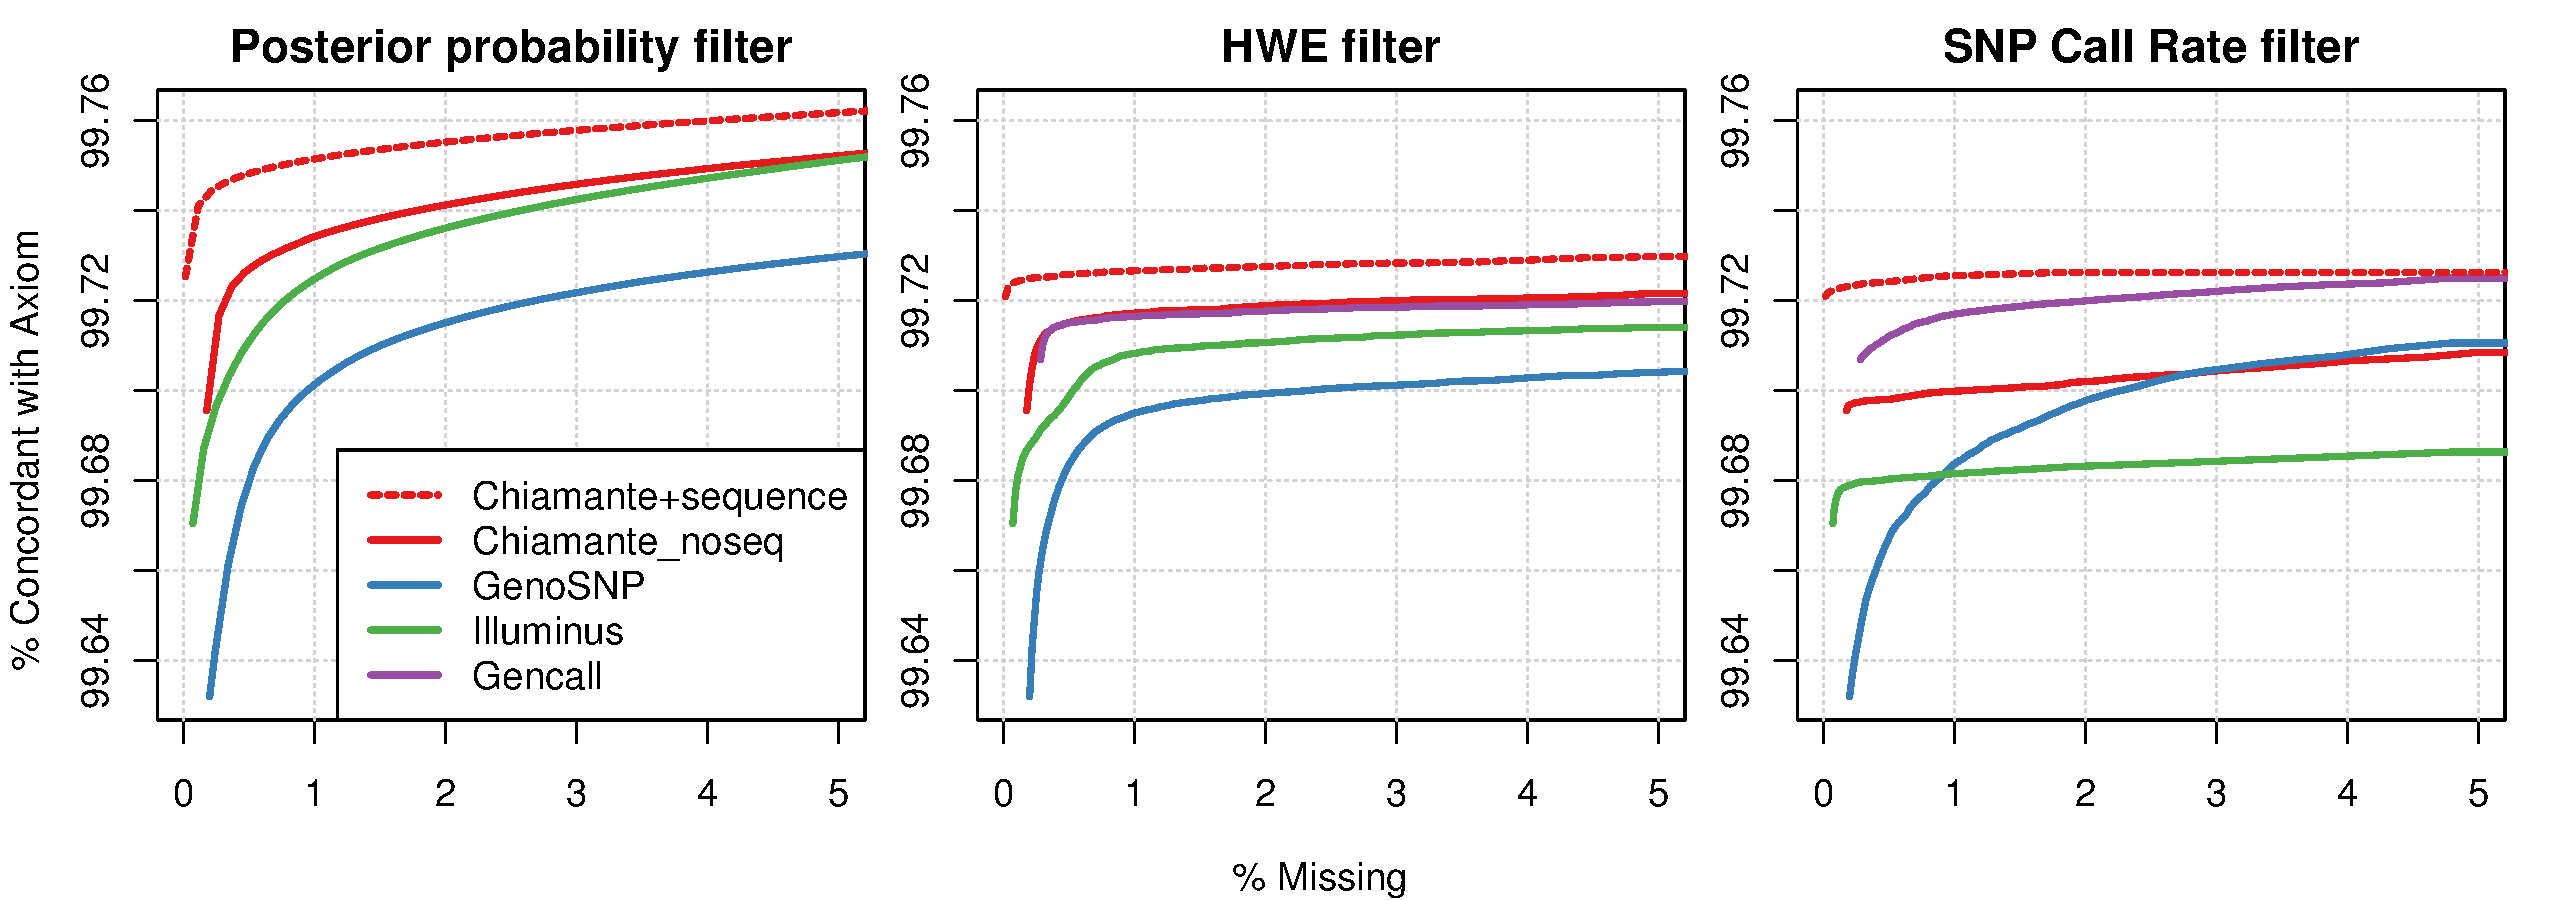
\includegraphics[width=\textwidth]{chap2figs/Fig2}
    \caption[Concordance against missingness for increasingly stringent QC filters]{Concordance against percentage missing data plots as increasingly stringent filter thresholds are applied. The left hand plot shows the effect of the filter on posterior probability (PP) of the methods Chiamante without using sequence data (red solid), Chiamante with use of sequence data (red dashed), GenoSNP (blue) and Illuminus (green). There is no comparison with GenTrain2 as the PP filter cannot be applied to this method. The middle plot show the effect of changing the threshold of the filter on HWE p-value. The right hand plot shows the effect of changing the threshold on the SNP call rate.\label{arrayfig}}
  \end{center} 
\end{figure}

\clearpage

\subsection{Data sets with a subset of samples with only array data and a subset of samples with both sequencing and array data} 

Having established that our method performs well in the situation in where only array data is available we investigated the gains in accuracy that could be achieved by utilising sequencing data on a subset of the samples. We again used the 1,525 individuals assayed on the Omni2.5S, 1,094 of these samples also have sequence data available. We applied our method with and without use of the sequence data. 

Table~\ref{tab_seq1,525}  shows the results of our method with and without the use of sequence data on the unfiltered data as well as all combinations of these filters. We examine performance on all 828 samples with Affymetrix Axiom data so that we can make a direct comparison with the results in Table~\ref{chap2:arrayconc} and shows clearly that overall the addition of sequence data leads to a clear boost in performance across a range of filtering options. When all the filters were applied the SCR, GCR and Concordance increase from 99.66, 99.487 and 99.727 to 99.954, 99.903 and 99.736. When sequence data is used the various filters have much less effect. For example, the GCR, SCR and Concordance never drop below 99.9\%, 99.95\% and 99.721\% respectively for any combination of filters. The fact that concordance does not seem to increase much (99.721\% without sequence data and 99.736\% with sequence data) maybe due to errors in the Axiom data that effectively put an upper bound on this measure that is below 100\%. 

\begin{table}[p]
\begin{center}
\begin{tabular}{|l|rrr|rrr|}
  \hline
  Method & \multicolumn{3}{c|}{Chiamante}& \multicolumn{3}{c|}{Chiamante+Sequence}\\
  \hline
  Filter & GCR & SCR & Conc & GCR & SCR & Conc \\ 
  \hline
  None & 99.824 & 100.000 & 99.696 & 99.986 & 100.000 & 99.721 \\ 
  GCR & 99.646 & 99.765 & 99.698 & 99.974 & 99.985 & 99.722 \\ 
  HWE & 99.766 & 99.941 & 99.708 & 99.970 & 99.984 & 99.723 \\ 
  PP & 99.744 & 100.000 & 99.715 & 99.940 & 100.000 & 99.733 \\ 
  \hline
  GCR+HWE & 99.590 & 99.710 & 99.709 & 99.958 & 99.969 & 99.723 \\ 
  PP+GCR & 99.520 & 99.694 & 99.722 & 99.914 & 99.966 & 99.734 \\ 
  PP+HWE & 99.696 & 99.940 & 99.722 & 99.927 & 99.986 & 99.734 \\ 
  \hline
  All & 99.486 & 99.659 & 99.726 & 99.903 & 99.954 & 99.736 \\ 
  \hline
\end{tabular}
\caption[Performance with and without and with the use of sequence data. ]{Comparison of Chiamante's performance applied to the 1,525 samples with data from the Illumina Omni2.5S chip without (left) and with (right) the use of sequence data. Genotype call rate (GCR), SNP call rate (SCR) and concordance (Conc) with the Affymetrix Axiom chip in \% are listed for each call set. Table rows correspond to a different combination of filters applied to the data. The PP filter removes all genotypes with a posterior probability below 0.9.  The HWE filter removes whole SNPs that show departures from HWE. The GCR filter removes whole SNPs where the call rate is below 0.9. Call rate is defined at the percentage of genotypes that were not ``NULL''.}
\label{tab_seq1,525}
\end{center}
\end{table}

\begin{figure}[p]
  \begin{center} 
    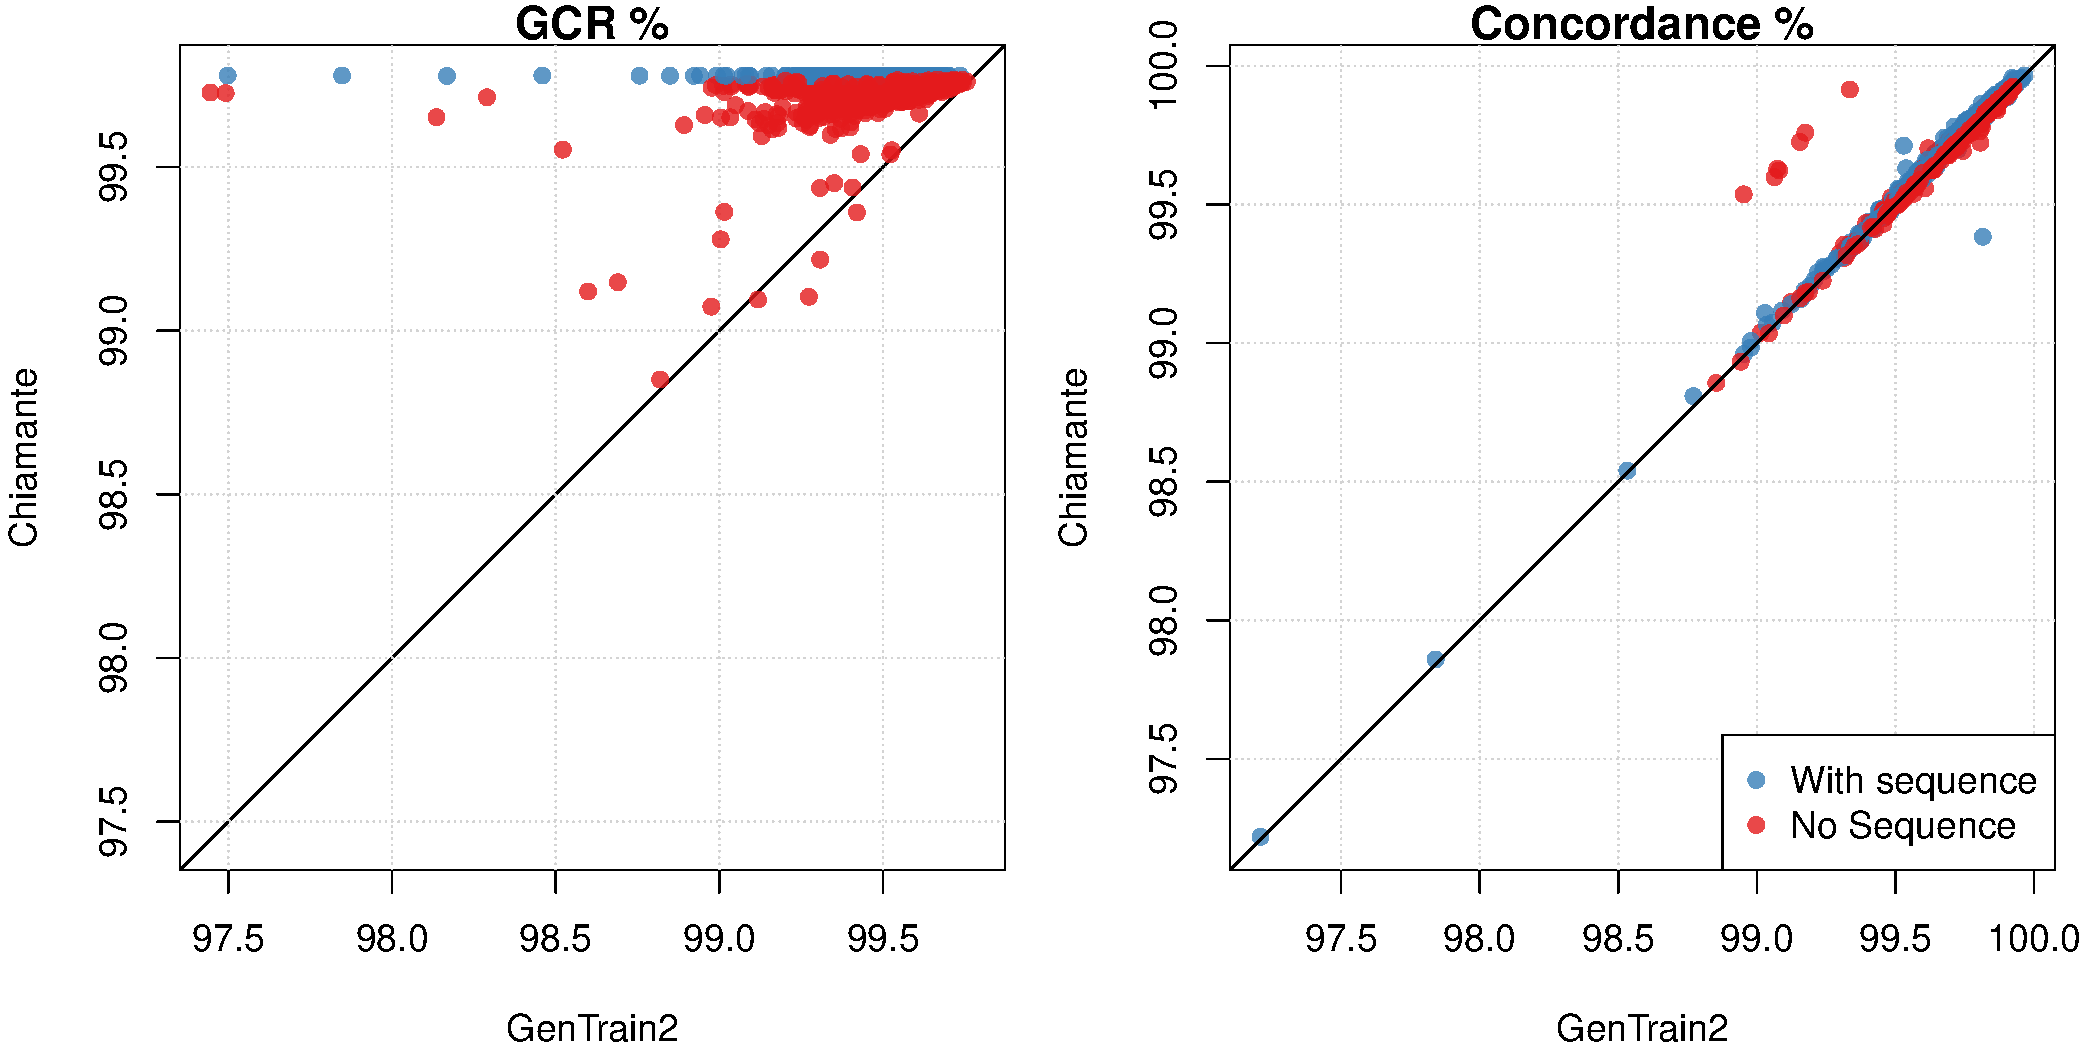
\includegraphics[width=\textwidth]{chap2figs/genotypecalling_byindv}
    \caption[Chiamante versus GenTrain2: per sample performance]{Chiamante+Sequence metrics versus GenTrain2 metrics for 828 individuals assayed on both microarrays.  The blue points are individuals that also have sequence data available, the red points are individuals whom were only assayed on microarrays. We can see that concordance is roughly the same between both methods but GCR is substantially larger for Chiamante+Sequence.  It is notable that there is improvement both for sequenced and non-sequenced samples.\label{seqnoseq}}
  \end{center} 
\end{figure}

Figure~\ref{arrayfig} shows the advantages of combining sequence and array data (red dotted line) compared to the methods that do not use sequence data via the missing data versus concordance plots. Figure~\ref{seq1,525qq} shows quantile-quantile plots for the HWE p-values for the different methods and further highlights that combining sequence and array data can noticeably reduce the number of SNPs failing HWE filters. Both highlight the ability of Chiamante+Sequence to improve call rate whilst maintaining accuracy.
\newpage
So far we have described metrics on 828 validation individuals, but 205 of these do not have any sequencing data available.  It is interesting to see if these individuals also have improved calls, or just the sequenced individuals. Figure~\ref{seqnoseq} plots metrics for Chiamante+Sequence versus GenTrain2 for each individual and colours points according to whether individuals are sequenced or not. There is improvement for individuals with no sequence data as well as the sequenced individuals,  we suspect this is due to the sequence data leading to improved model fit, hence benefiting all samples. In table~\ref{chap2:results:splitchi} we have split the results on the 828 samples with Axiom data into the subset of 623 that have 4X sequence data available and the remaining 205 samples that have no sequence data. The GCR and Concordance on the 205 samples are 99.423\% and 99.728\% when no sequence data is used and all post-calling filters have been applied. When sequence data is used on the calling the GCR rises by 0.4\% to 99.841\% and there is a slight rise in Concordance to 99.732\%.

Perhaps of greatest interest are the gains that can me made from using a combination of array and sequence at low frequency variants.  To evaluate this we took sites with a minor allele frequency less than 0.05 across all populations (estimated from the Axiom data) giving us 62,666 loci with 33,759,388 genotype calls (31,807,602 major homozygotes, 1,868,371 heterozygotes and 83,415 minor homozygotes). 

We then calculate sensitivity and specificity for each genotype $j$ and method, where
$$\textrm{Sensitivity}_j = 100 \times  \frac{\sum_{i=1}^N I(\hat{G}_{i=1} = j)I(G^{\textrm{Axiom}}_{i=1} = j)}{ \sum_{i=1}^N I(G^{\textrm{Axiom}}_{i=1} = j)} \qquad j \in (0,1,2,\textrm{NULL}))$$
$$\textrm{Specificity}_j = 100 \times  \frac{\sum_{i=1}^N I(G_{i=1} = j)I(G^{\textrm{Axiom}}_{i=1} = j \cap G^{\textrm{Axiom}}_{i=1} \neq \textrm{NULL})}{ \sum_{i=1}^N I(\hat{G}_{i=1} = j \cap G^{\textrm{Axiom}}_{i=1} \neq \textrm{NULL})}$$
that is, sensitivity is the percentage of the ``true genotypes'' (defined by Axiom) called by a method whilst specificity is the percentage of genotypes called by a method that are correct. 
\newpage
In this low frequency scenario we see more substantial improvements. The results are shown in Table \ref{1094tab4}. Chiamante (with sequence) has consistently higher detection rate and lower false positive rate for all genotypes compared to the other methods.  In particular, we identify an extra 0.3\% minor homozygotes with 1.8\% fewer false positives compared to GenoSNP (the next best method for minor homozygotes).  We detect an additional 0.27\% heterozygotes with 0.25\% fewer false positives compared to GenCall, the next best method for heterozygotes. It is important to note here that the Axiom chip is also likely to be inaccurate for low frequency variants hence the error rate will be inflated, however this is still a reasonable way to compare each method on a relative scale. Illuminus has a much lower specificity 80.4\% on minor homozygotes than all the other methods which are all above 88.7\%.  
\begin{table}
\begin{center}
\begin{tabular}{|ll|c|c|}
  \hline
%  & &Sensitivity (\%)  & Specificity (\%)\\ 
% Method & Genotype (G) &  $100 \times P(Call = G | Axiom = G)$ & $100 \times P(Axiom = G | Call = G)$ \\
 Method & Genotype (G) &TPR (\%) & 1-FPR (\%)\\
 \hline
          & Major homozygote   & 99.78178 & 99.90596 \\
 Chiamante& Heterozygote     & 98.11328 & 98.65827 \\
          & Minor Homozygote   & 95.62908 & 88.78019 \\
 \hline
                   & Major homozygote    & 99.94782 & 99.90693 \\
 Chiamante+Sequence& Heterozygote     & 98.25222 & 99.19872 \\
                   & Minor Homozygote       & 96.11221 & 90.87426 \\
 \hline   
          & Major homozygote    & 99.78903 & 99.90625 \\
 GenoSNP & Heterozygote    & 97.95581 & 98.26359 \\
          & Minor Homozygote    & 95.81610 & 89.10256 \\
 \hline
          & Major homozygote    & 99.80620 & 99.90755 \\
 Illuminus& Heterozygote      & 97.38227 & 98.06591 \\
          & Minor Homozygote    & 95.28982 & 80.46608 \\
\hline
        & Major homozygote        & 99.67136 & 99.90829 \\
 GenCall& Heterozygote     & 97.98680 & 98.94823 \\ 
        & Minor Homozygote      & 95.60631 & 89.88650 \\
 \hline

\end{tabular}
\caption[Genotype calling performance at low frequency SNPs]{Sensitivity and specificity per genotype (for variants with MAF $<$ 0.05) for different calling methods using array data (and in Chiamante's case, sequence data) from 1094 individuals with validation data on a subset of 623 of these individuals.  Chiamante calls a higher rate of the low frequency variants whilst maintaining better sensitivity (true positive rate) and specificity (1 - false positive rate).}
\label{1094tab4}
\end{center}
\end{table}

\clearpage
To further illustrate the performance of our method and the benefit of using sequence and array data together Figure~\ref{chap2:fig:scatterplots} shows the cluster plots for three example SNPs shown on the three rows of the plot. The first column shows the cluster plots with points coloured using a RGB colour scheme based on the scaled GLs. In this way points that are very clearly coloured red, green and blue indicate genotypes where sequence data strongly supports reference homozygotes, heterozygotes and alternate homozygotes respectively. Genotypes for which the GLs are relatively flat across genotypes will be plotted as a mixture of red, green and blue. This way of plotting points helps to illustrate the general agreement between intensity clusters and GLs. The next three columns show the calls made by Chiamante, Illuminus and GenoSNP respectively. 

The first row shows an `easy' SNP where all methods agree. The second row shows a SNP where there are several points that lie between obvious clusters that could be hard to classify using array data alone. Here the use of sequence data leads to a boost in concordance by correctly classifying these ambiguous points. The third row shows a challenging SNP with atypical cluster centroids and where Allele 2 has low frequency, resulting in very few rare homozygotes which makes model fitting to array data only quite challenging. The concordance of Chiamante is considerably higher on this SNP due to both the use of sequence data and the priors we use on cluster locations which contribute to this increase in accuracy at rare SNPs.

\clearpage
\changepage{}{}{-.5in}{-.5in}{}{}{}{}{}
%\begin{landscape}
\begin{figure}
  \begin{center} 
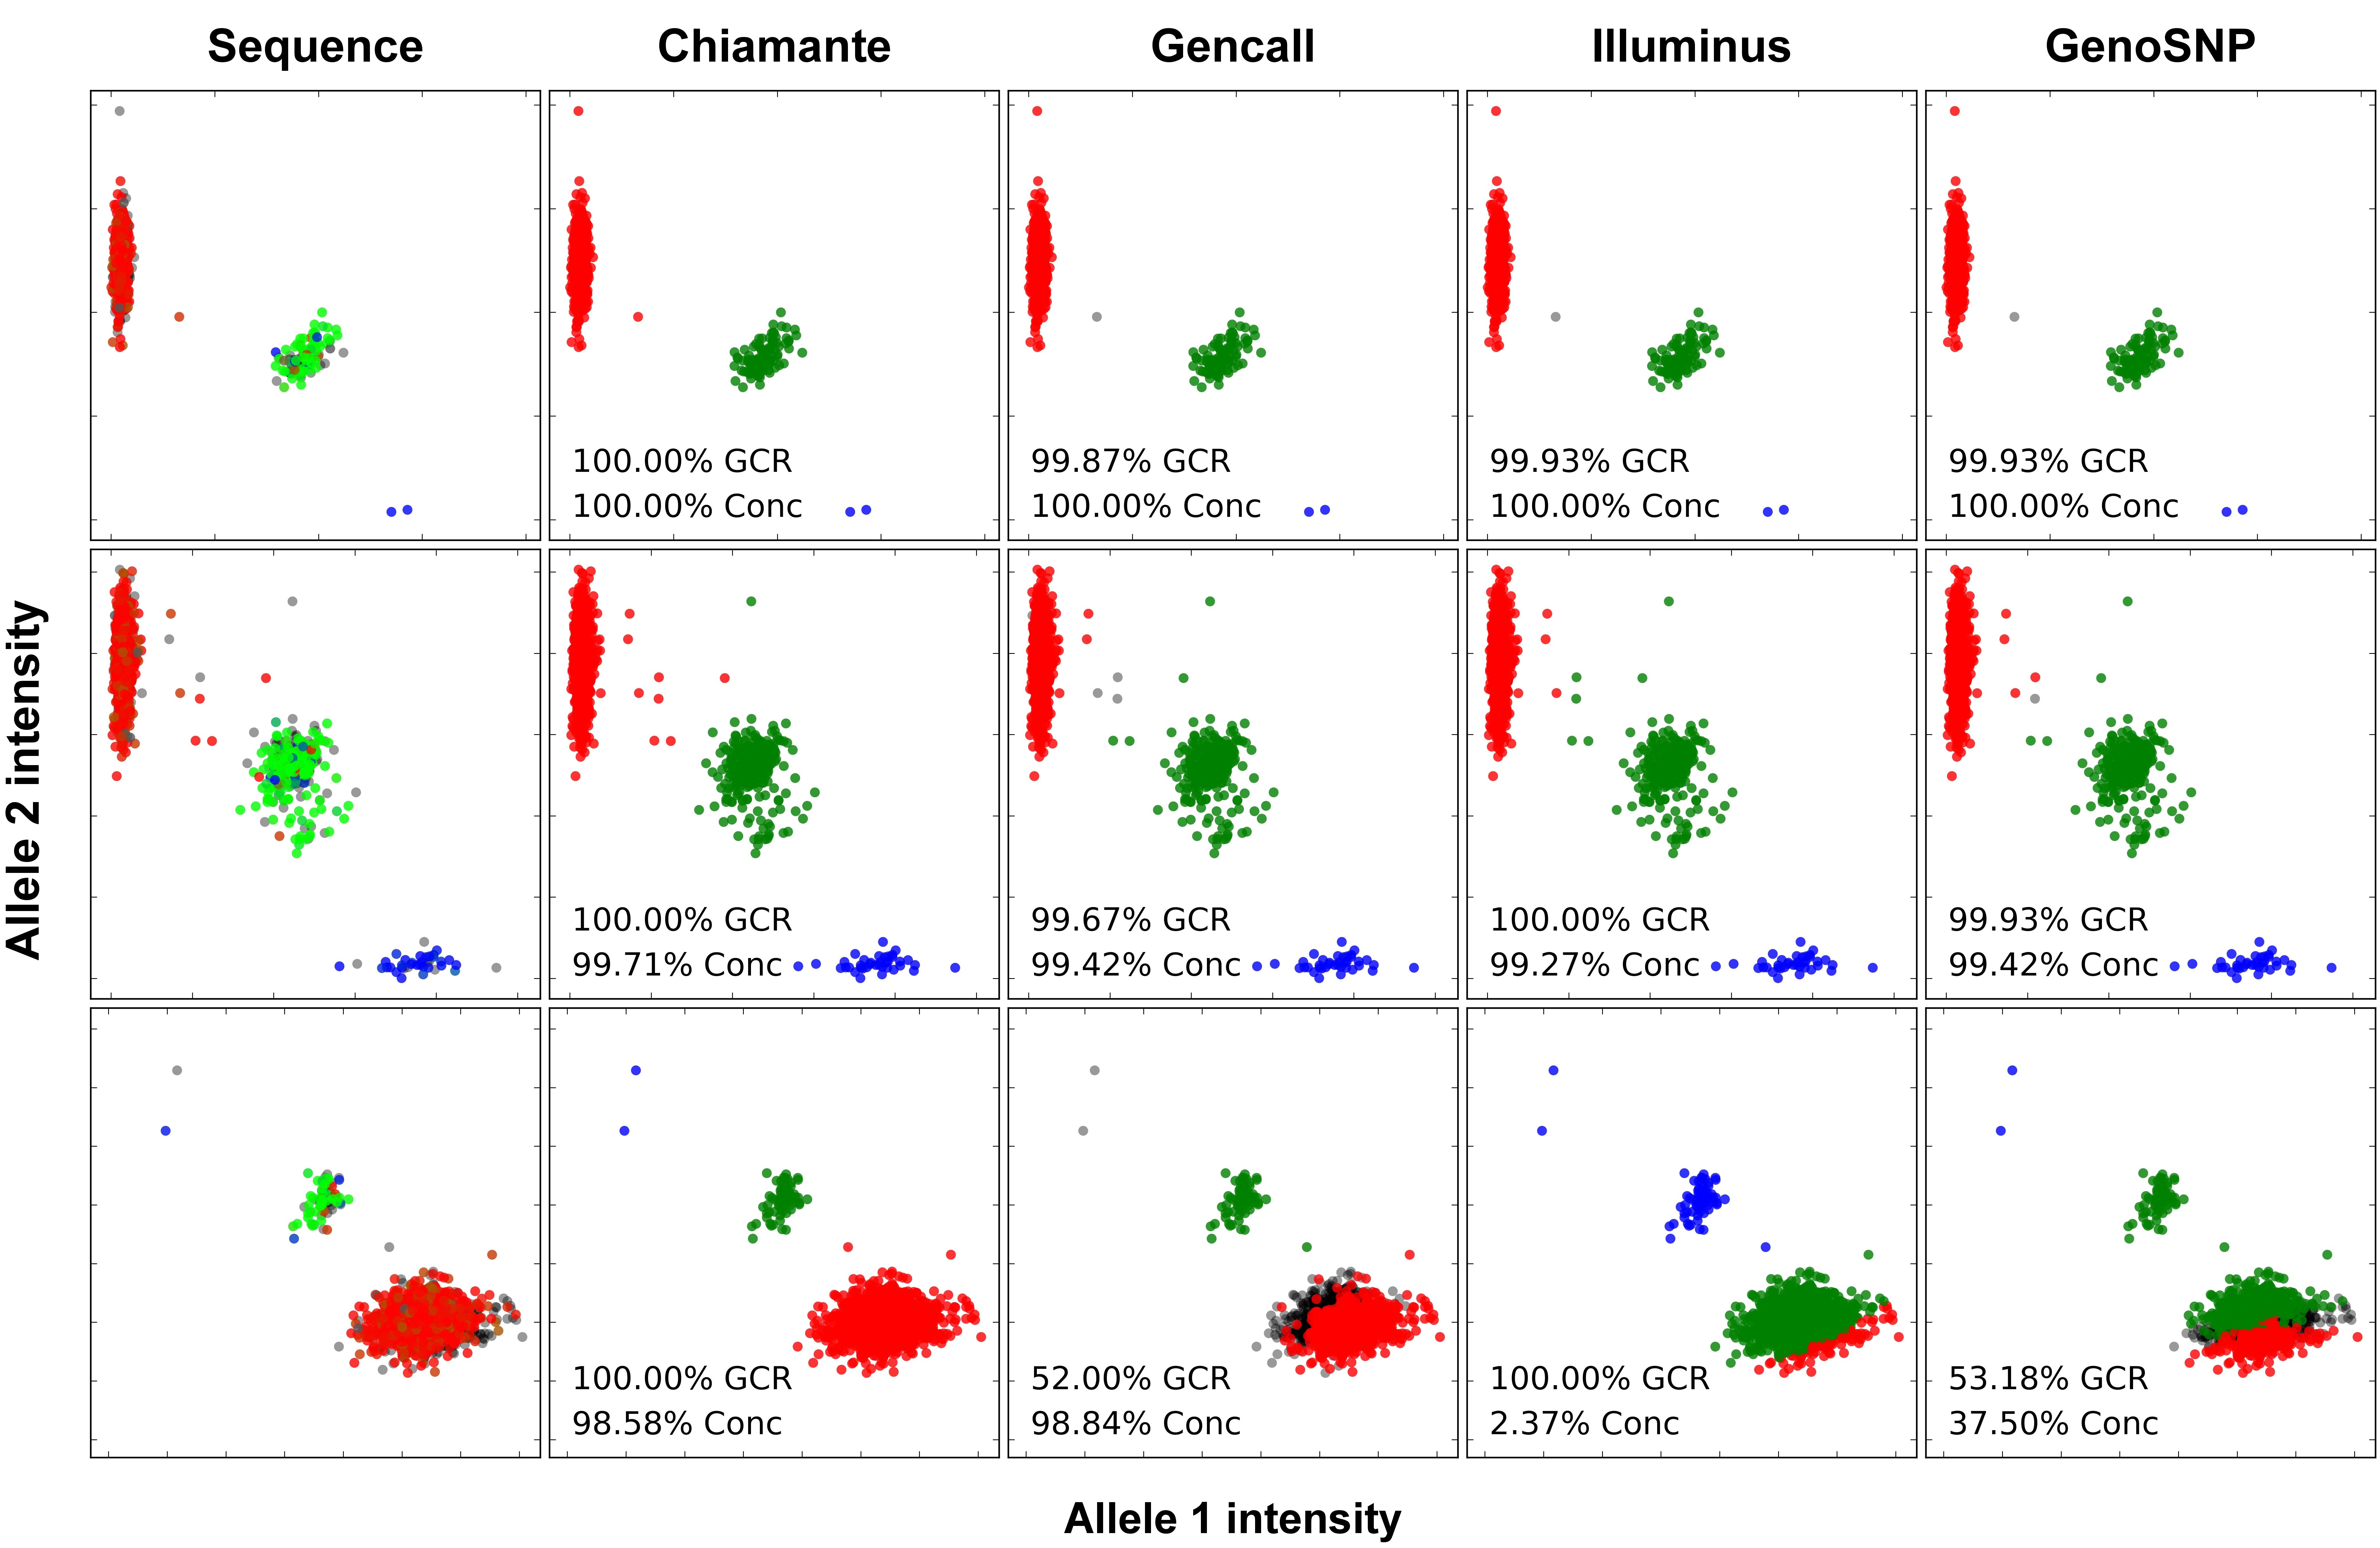
\includegraphics[width=\textwidth]{chap2figs/Fig4}
\vspace{-10pt}
    \caption[Scatter plots of allele intensities at three different loci of varying difficulty]{Scatter plots of allele intensities at three different loci.  In the far left column, points are coloured using a RGB colour scheme based on the scaled GLs. In this way points that are very clearly coloured red, green and blue indicate genotypes where sequence data strongly supports reference homozygotes, heterozygotes and alternate homozygotes respectively. Note the first probe of the Omni2.5S chip can be for either the reference or alternate allele so the colour of the homozygotes can differ between loci. Genotypes for which the GLs are relatively flat across genotypes will be plotted as grey.  The other four columns are coloured by genotypes from call sets generated by the respective algorithms. \textbf{Top:} Intensities from a typical well clustered SNP. The array-only methods call genotypes accurately but with one missed call.  Chiamante can `mop up' such ambiguous micro-array assays by exploiting the sequence information for this sample resulting in a higher call rate than the other callers. \textbf{Centre:} A more difficult SNP.   There are several uncertain samples between clusters which the other callers misclassify or exclude as missing, Chiamante can use the sequence information to accurately call these samples.  \textbf{Bottom:}  A SNP with relative low allele 2 frequency.  Illuminus and GenoSNP have both completely failed at this locus (this is likely due to incorrect convergence in the Illuminus case) whilst GenTrain2 has a large amount of missing data.  This SNP would typically be filtered in any reasonable QC pipeline.  The sequence data drives Chiamante to the correct parameter estimates for the mixture distribution resulting in accurate classification and high call rate at this locus.\label{chap2:fig:scatterplots}}
  \end{center} 
\end{figure}
%\end{landscape}
\changepage{}{}{+.5in}{+.5in}{}{}{}{}{}

\clearpage
\subsection{Examining errors}
\label{chap2:results:errors}
Our method estimates the rate at which the sequence and array assays have ``failed'' at each locus via the $\eta_Y$ and $\eta_X$ parameters respectively. Figure~\ref{chap2:results:eta_hist} shows histograms of these parameter estimates for all of the SNPs that were on the Illumina Omni2.5S chip and in the 1000 Genomes Phase I call set. The failure rate parameter for the sequence assay is noticeably elevated compared to the array assay. The majority of SNPs have an estimated sequence assay failure of between 0.001-0.0001, while  for the array assay the failure rates are almost always below 0.0001. 

We found that there were 754 SNPs with  $\eta_Y > 0.5$ but only 33 of these SNPs were on the Axiom array. Figure~\ref{chap2:results:eta_seq}  compares the properties of the calls at these SNPs with and without the use of sequence data. For the majority of the SNPs the calls are very similar with and without the use of sequence data, due to the sequence information being mostly discarded by the model.  There are some SNPs where the use of sequence data has led to greater divergence from HWE and some where the sequence data has modestly improved concordance. This suggests that model is largely robust to problematic sequencing data. Figure~\ref{seq_fail_1} shows a SNP flagged as having erroneous sequence level data ($\eta_Y = 0.63$). There is clear signal from the array assay showing good cluster separation whilst the sequencing data appears heavily biased towards the reference.  The model has correctly discarded the sequence data for many individuals at this locus and made high quality genotype calls (100\% Axiom concordance and call rate).

Figure~\ref{chap2:results:eta_array} shows various metrics for 235 SNPs that have the array failure rate,  $\eta_X > 0.5$ for Chiamante with and without sequence. The introduction of sequence data improves metrics on average, the HWE p-values are less extreme and both GCR and concordance are higher.  However call rates and concordance are frequently too low for these loci to be useful. Figure~\ref{array_fail_1} shows a typical example SNP flagged as having erroneous array level data ($\eta_X = 0.71$). There are a large number of points with 0 intensity, for most values here the genotype will be derived purely from sequence data.  The high concordance (98.6\%) should be considered in light of the very low call rate (73.9\%).  Such a locus is unlikely to be useful regardless of the calling method and would be filtered due to high missingness.

We have shown that our method is quite robust to extreme cases where the majority of sequencing or array data at a particular locus is spurious.  However these loci still tend to be of relatively poor quality and it may be to desirable to filter them.  Hence the two failure parameters may also be useful as quality control measures.  We calculated the average concordance for binned values of $-\log_{10}(\eta_X)$ and $-\log_{10}(\eta_Y)$ for Chiamante with and without sequence.   Figure \ref{fail_filtering} plots these averaged concordances against $-\log_{10}(\eta_X)$ and $-\log_{10}(\eta_Y)$.  The left panel shows how concordance changes with the array failure parameter, when sequencing data is present concordance is largely maintained even when array quality is low. However high values of $\eta_X$ will also lead to a large amount of missing values and SNPs are likely to be filtered on those grounds. The right plot shows concordance across the range of sequence failure rates, even when sequencing data is of poor quality Chiamante still benefits from its presence.  That said, low values of $\eta_Y$ tend to imply poor quality SNPs making this a useful QC parameter.  Filtering on $-\log_{10}(\eta_Y) <  2$ may be prudent and would result in the removal of only very few SNPs as can be seen in the histograms in Figure~\ref{chap2:results:eta_hist}.

\begin{figure}[p]
  \begin{center} 
    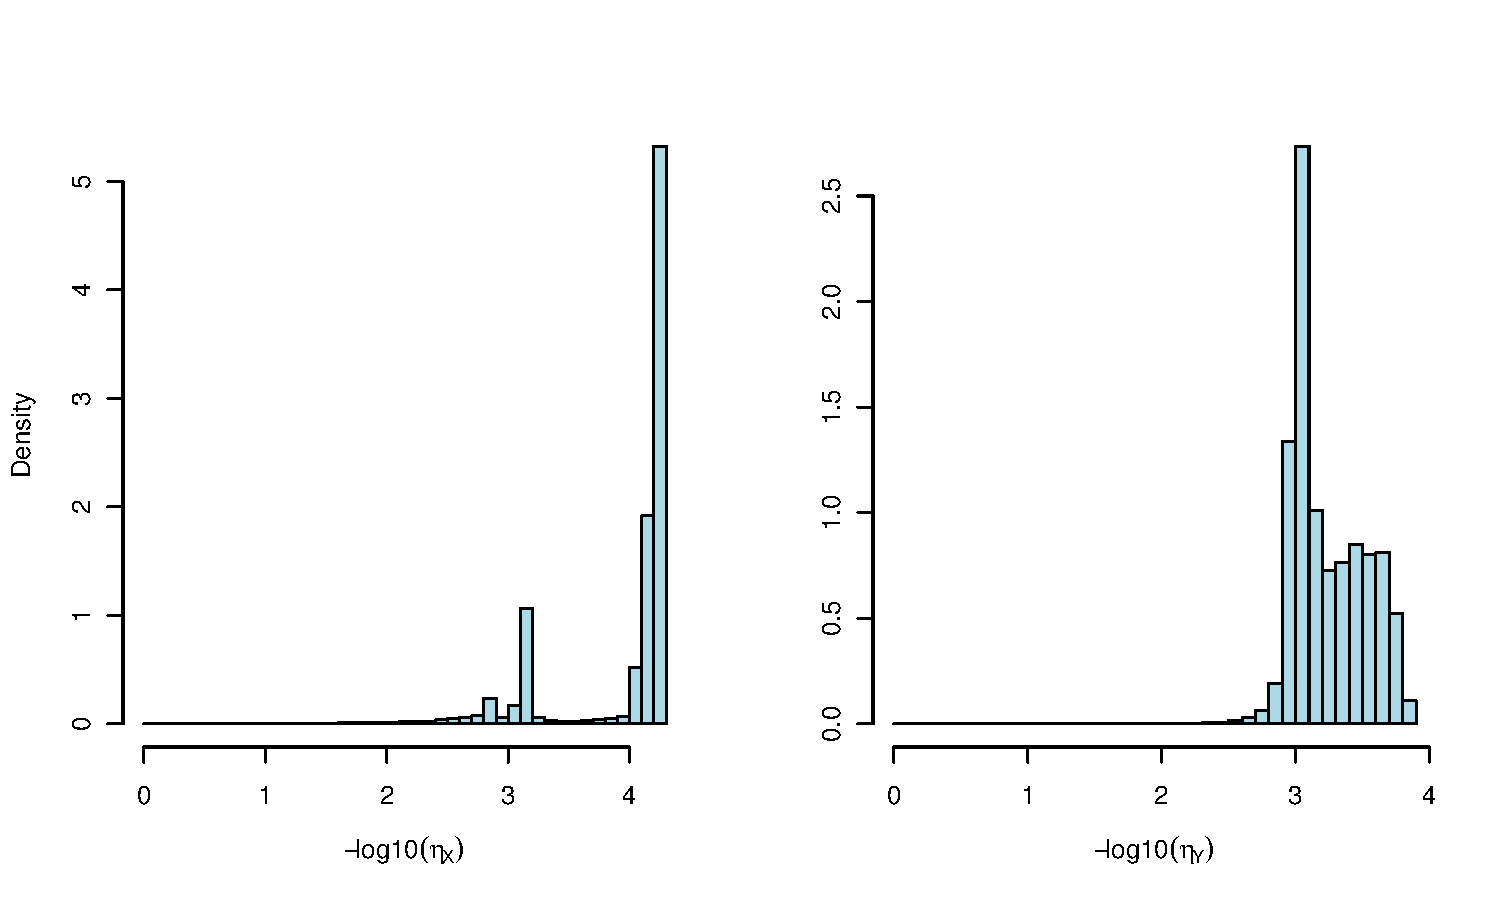
\includegraphics[width=\textwidth]{chap2figs/SupFig9}
    \caption[Histograms of the estimated failure rate parameters]{Histograms of the estimated failure rate parameters $-\log_{10} \eta_X$ for array assays (left) and $-\log_{10} \eta_Y$ for sequence assays (right).\label{chap2:results:eta_hist} }
  \end{center} 
\end{figure}


\begin{figure}[p]
  \begin{center} 
    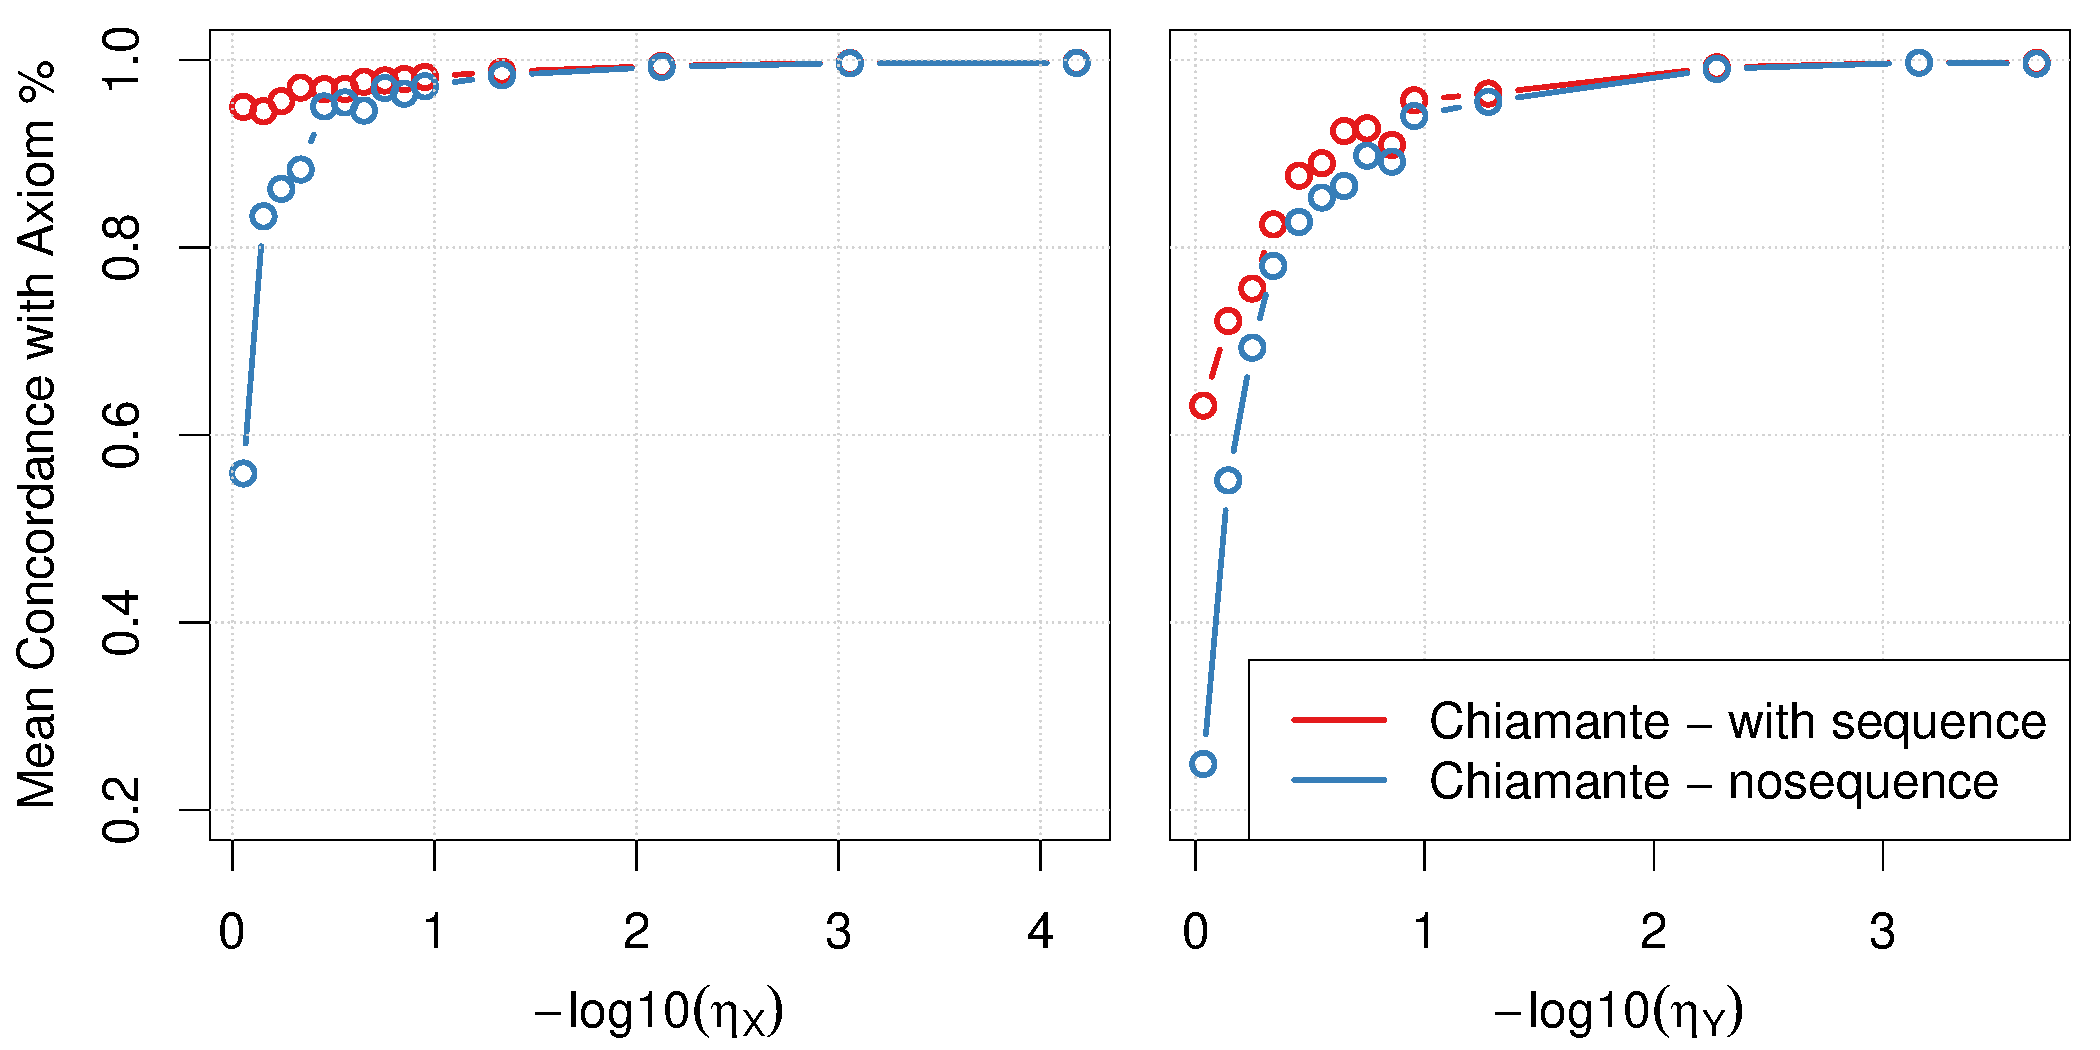
\includegraphics[width=\textwidth]{chap2figs/fail_filtering}
    \caption[Genotype concordance against rate of assay failure]{\textbf{Left:} Average concordance with Axiom against $-\log_{10} \eta_X$, the rate of array failure. \textbf{Right:} Average concordance with Axiom against $-\log_{10} \eta_Y$, the rate of sequence failure. Filtering SNPs with values of $-\log \eta_Y < 2$ may be a good additional QC measure.     \label{fail_filtering}}
  \end{center} 
\end{figure}

\begin{figure}[p]
  \begin{center} 
    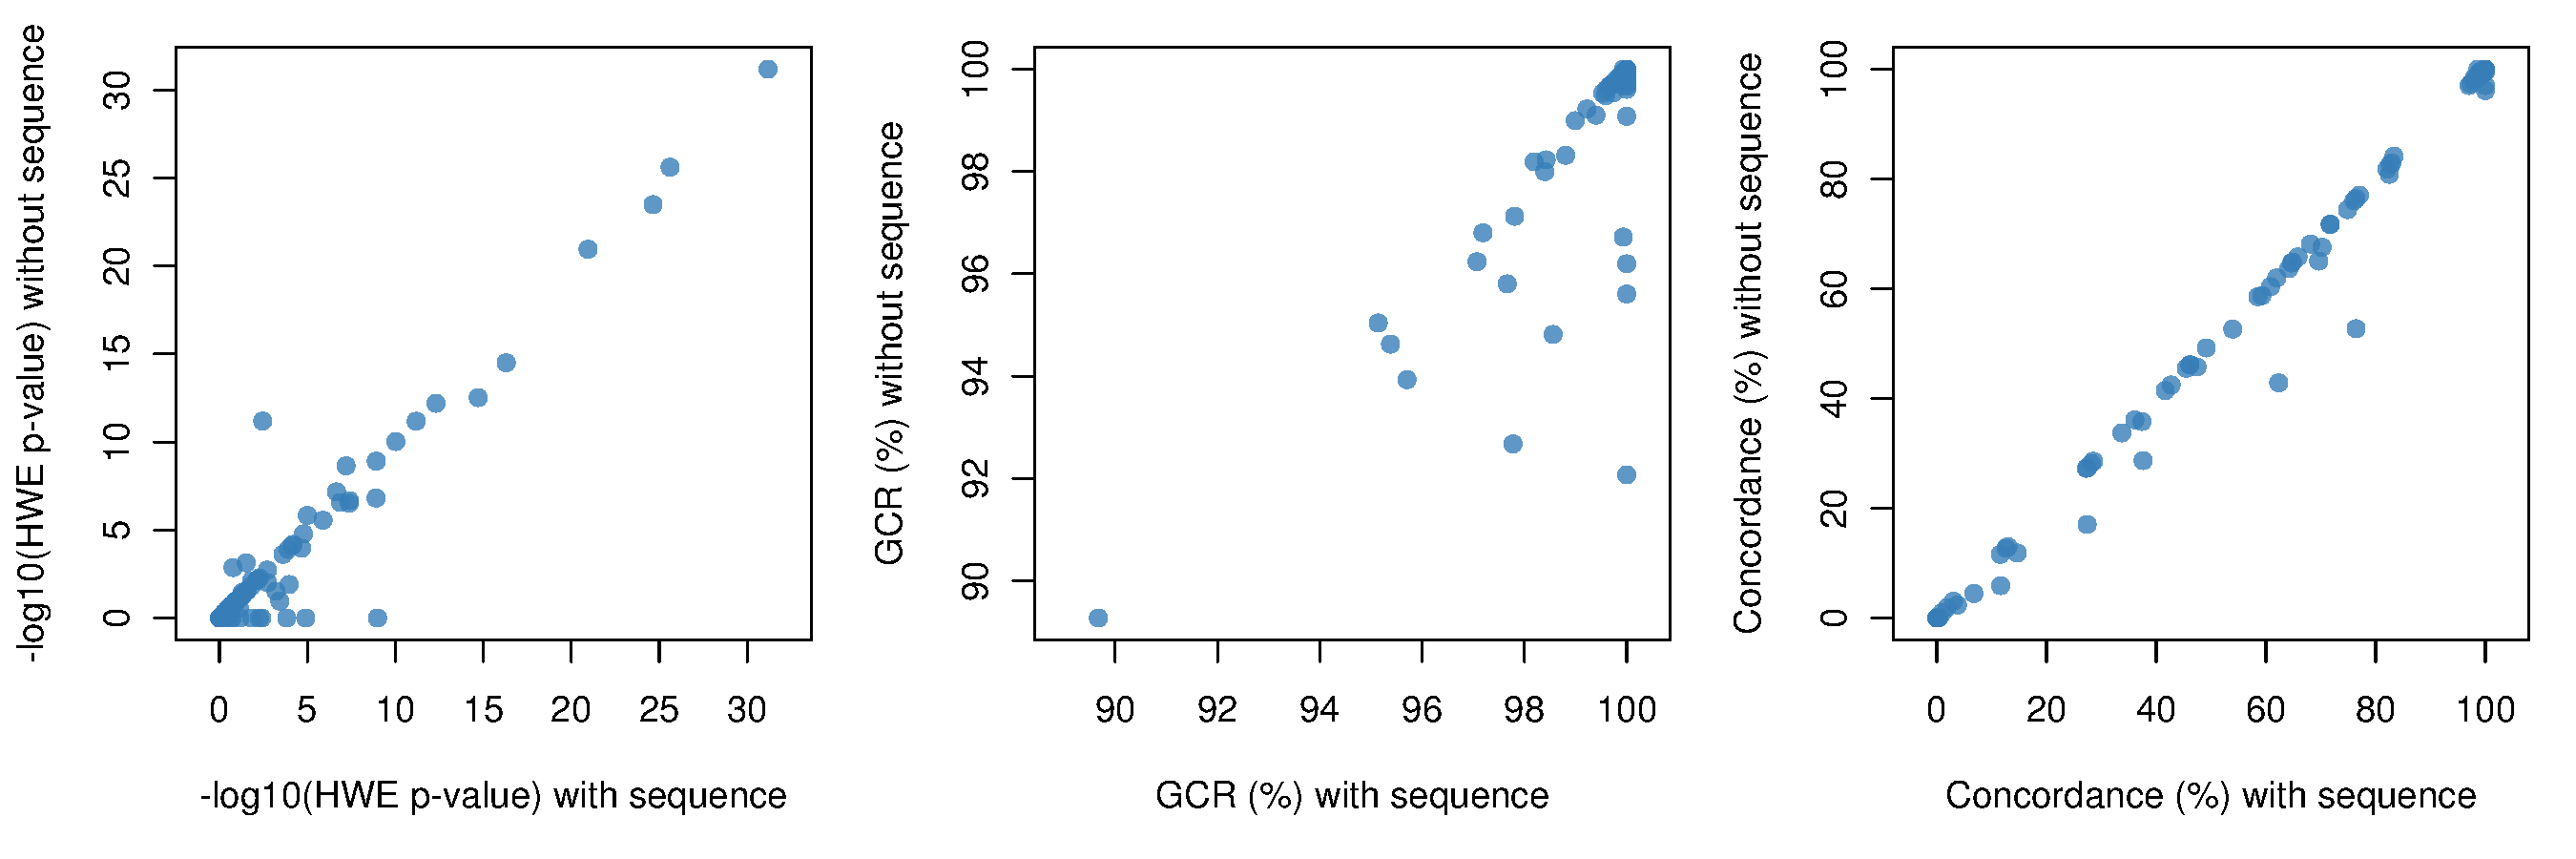
\includegraphics[width=\textwidth]{chap2figs/SupFig10}
    \caption[Evaluation of genotype calling when sequence data is problematic]{Comparison of calling with (x-axes) and without (y-axes) the use of sequence data on the 33 SNPs on the Axiom chip with high sequence failure rate, $\eta_Y > 0.5$. Left :  $-\log_10$ p-value for HWE. Middle : GCR. Right : Concordance.
      \label{chap2:results:eta_seq} }
  \end{center} 
\end{figure}


\begin{figure}[p]
  \begin{center} 
    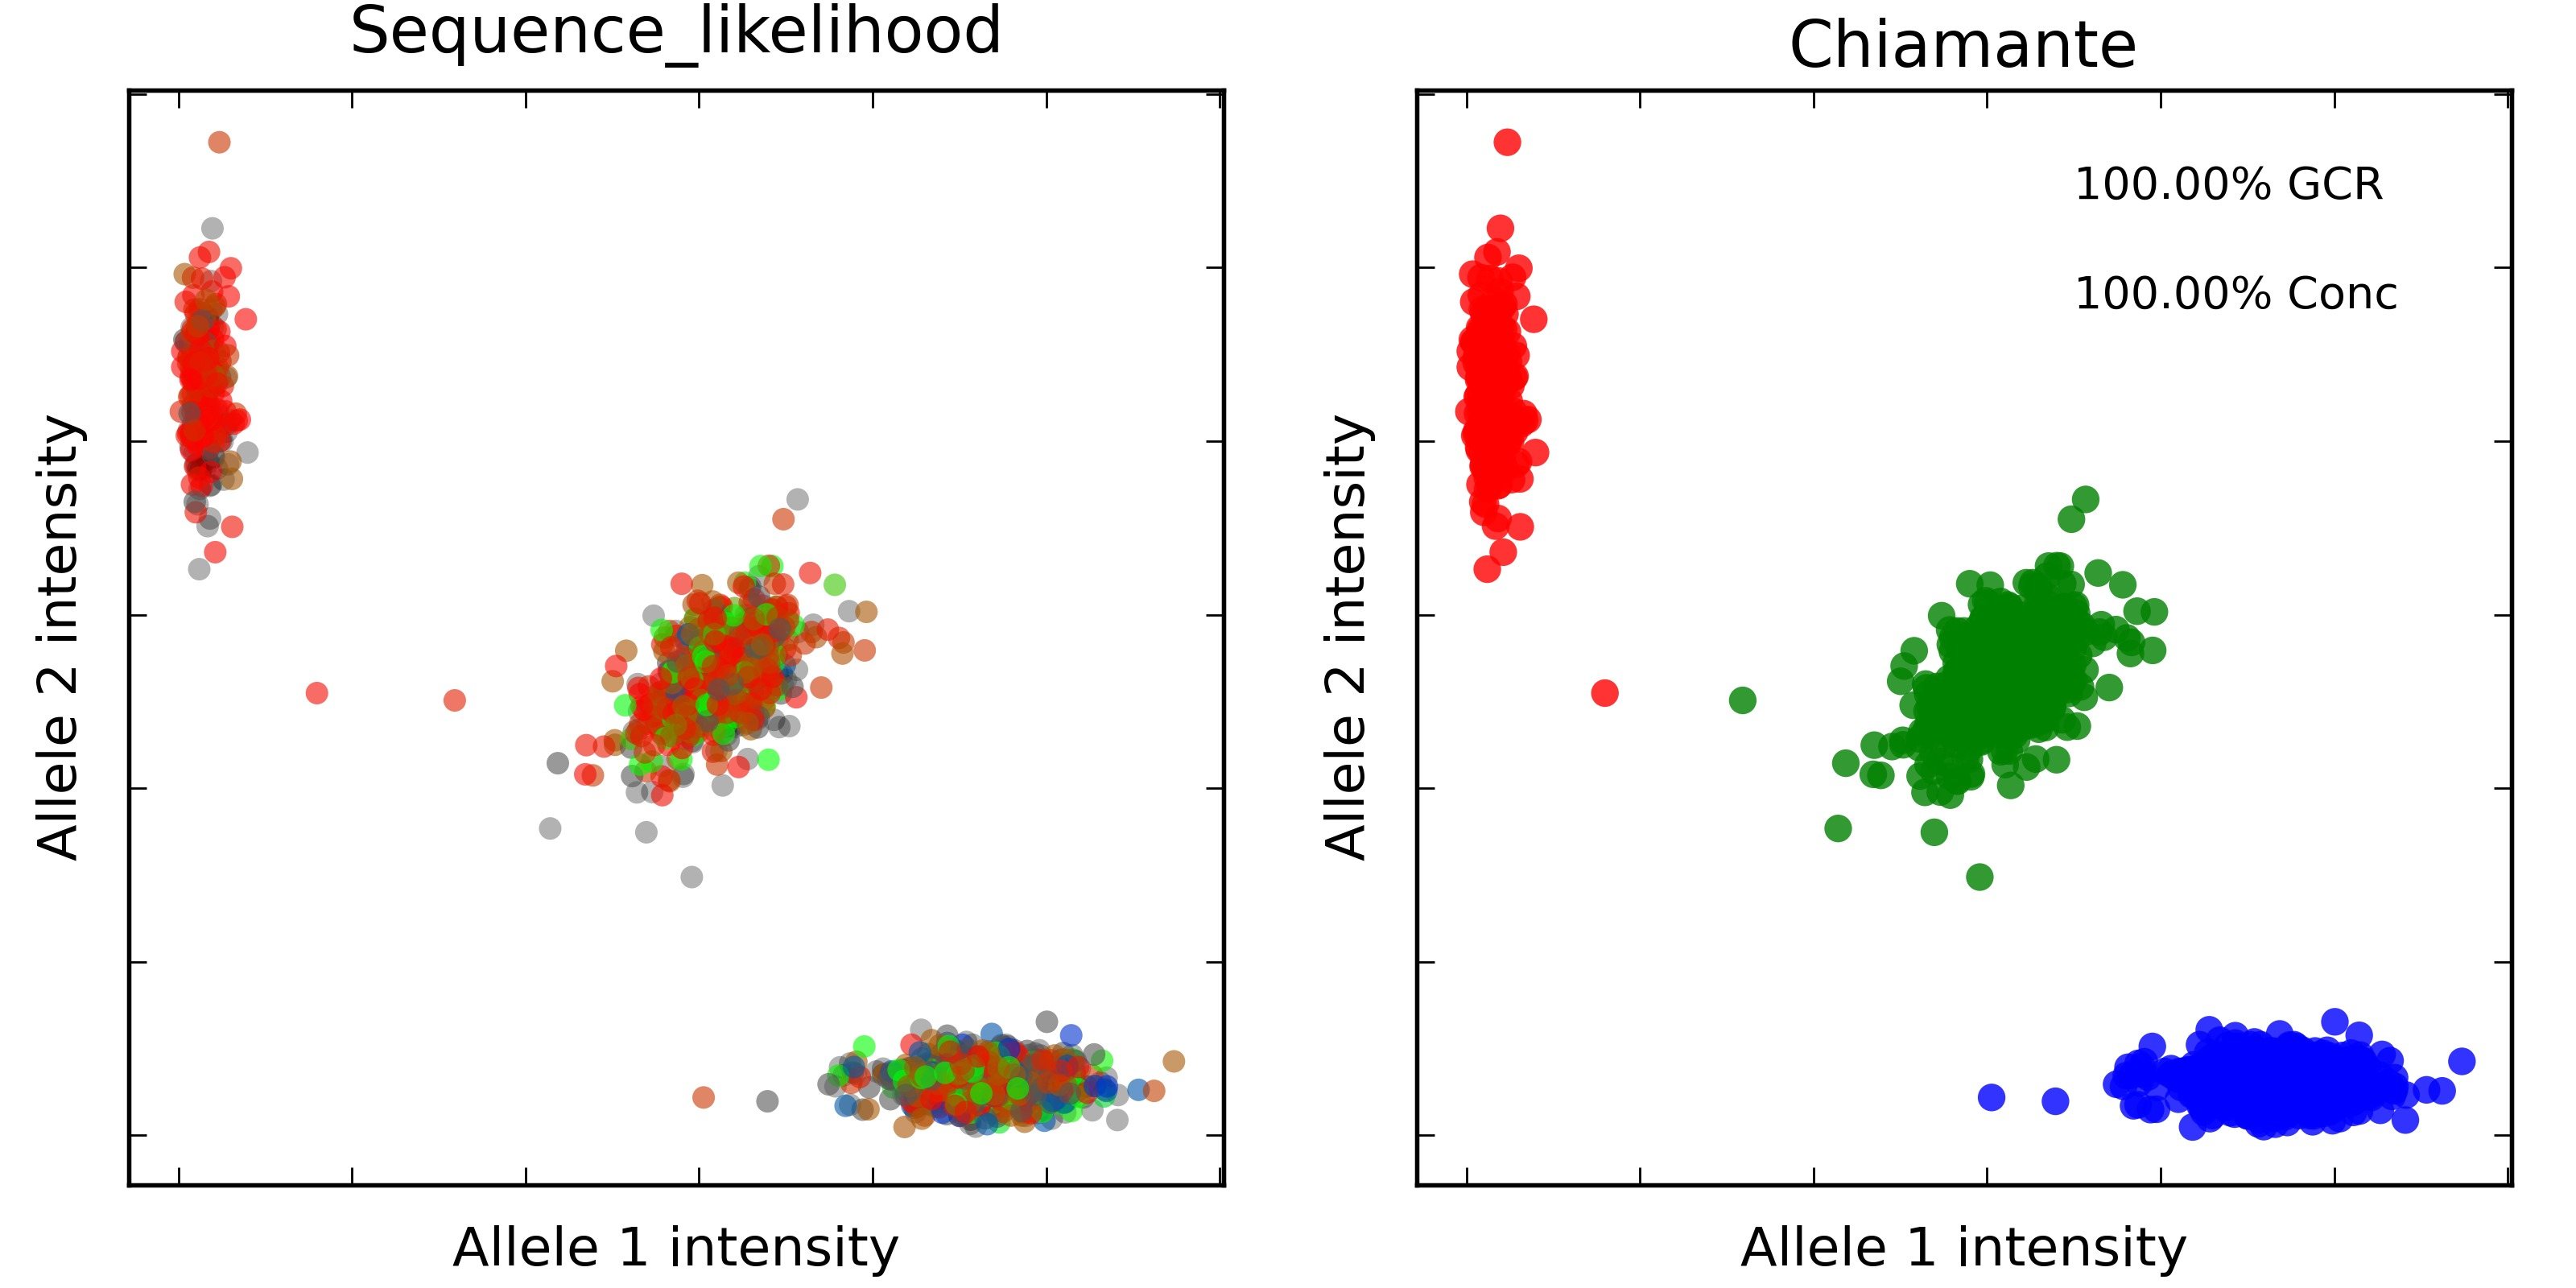
\includegraphics[width=\textwidth]{chap2figs/Fig5}
    \caption[Illustration of a SNP with high estimated sequence failure]{Illustration of a SNP with high estimated failure rate for the sequence assay ($\eta_Y = 0.63$). The left plot shows the cluster plot for the SNP with points coloured using a RGB colour scheme based on the scaled GLs for each genotype. The right hand plots shows the same cluster plot with points coloured according to the Chiamante posterior probabilities.\label{seq_fail_1}}
  \end{center} 
\end{figure}



\begin{figure}[p]
  \begin{center} 
    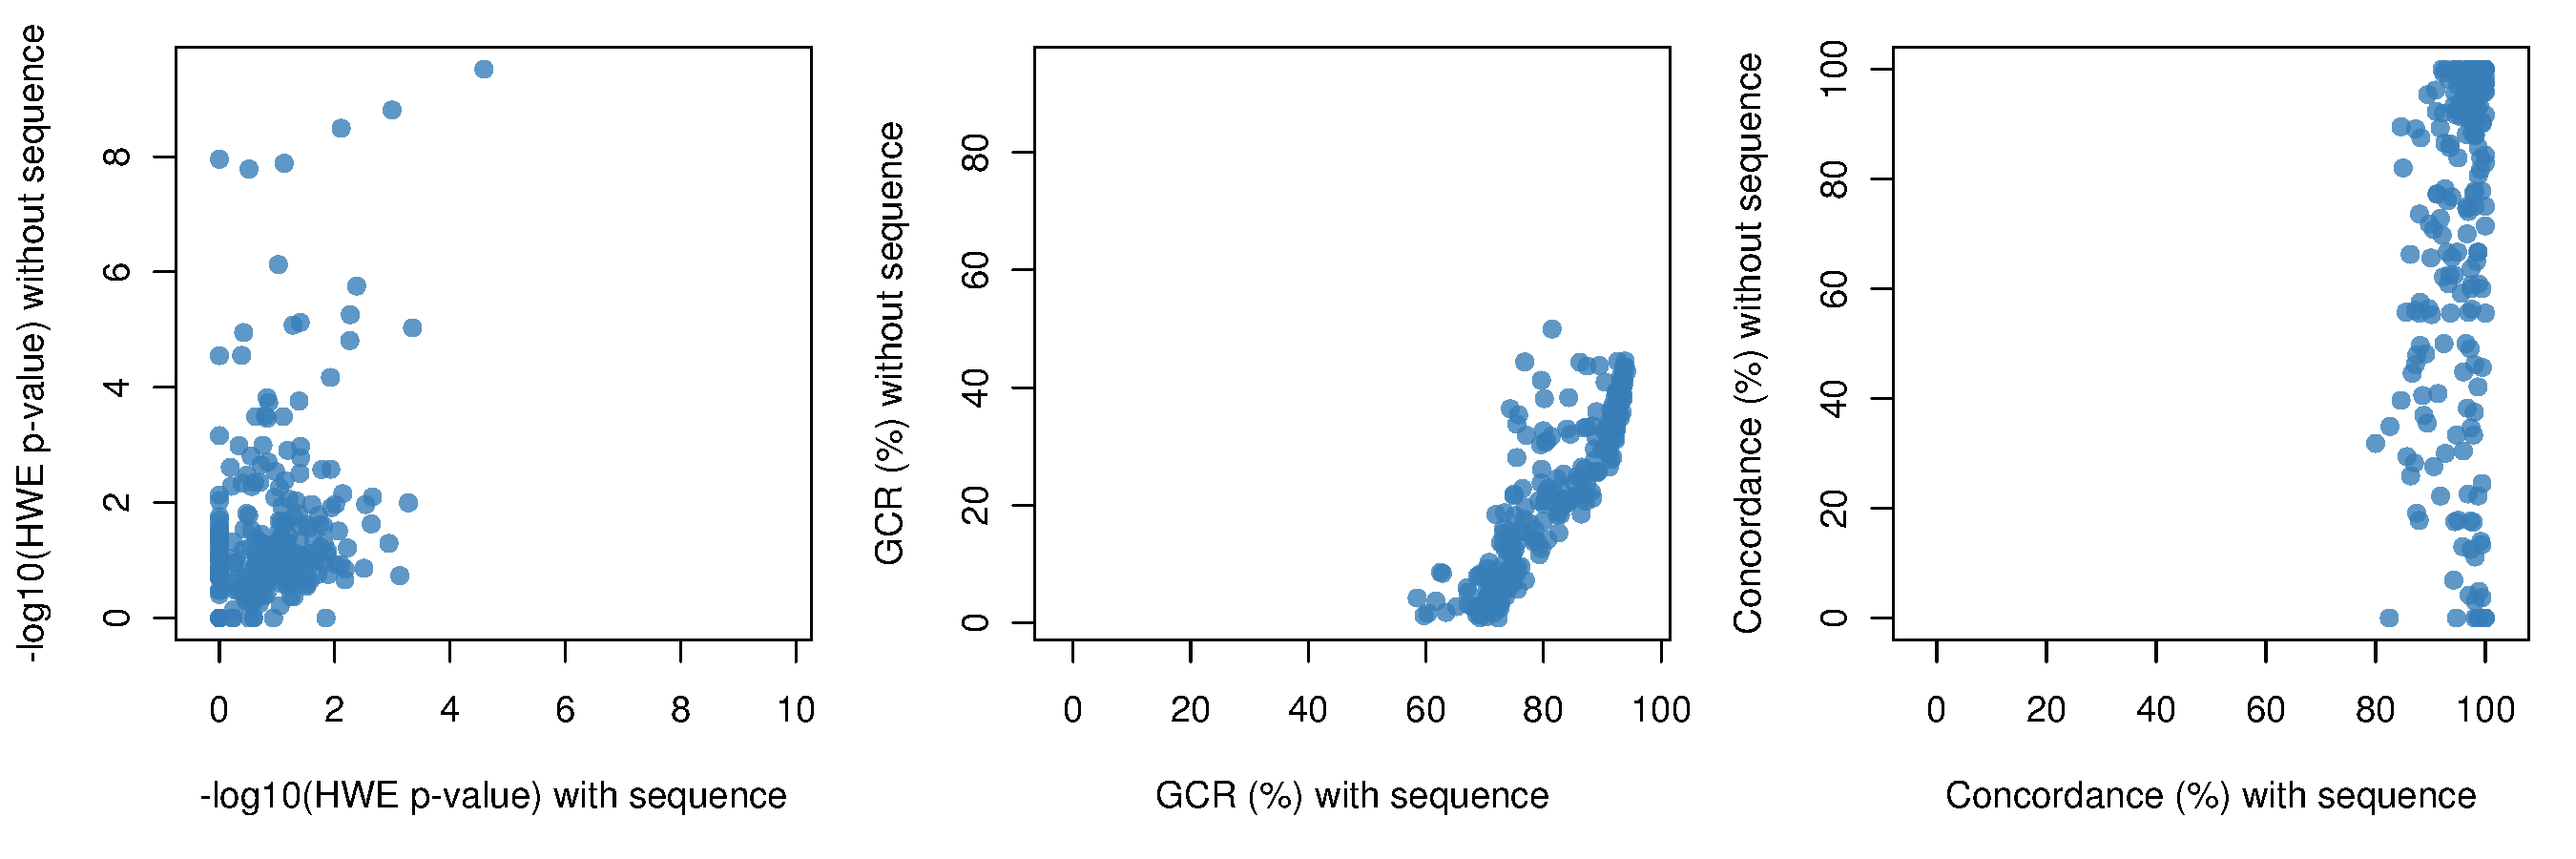
\includegraphics[width=\textwidth]{chap2figs/SupFig11}
    \caption[Evaluation of genotype calling when array data is problematic]{Comparison of metrics on the 235 SNPs called with high array failure rate, $\eta_X> 0.5$ . Plots of $-\log_{10}(\textrm{HWE p-value})$ (top), GCR (middle) and concordance (bottom) on these SNPs called with and without the use of sequence data.
      \label{chap2:results:eta_array}}
  \end{center} 
\end{figure}

\begin{figure}[p]
  \begin{center} 
    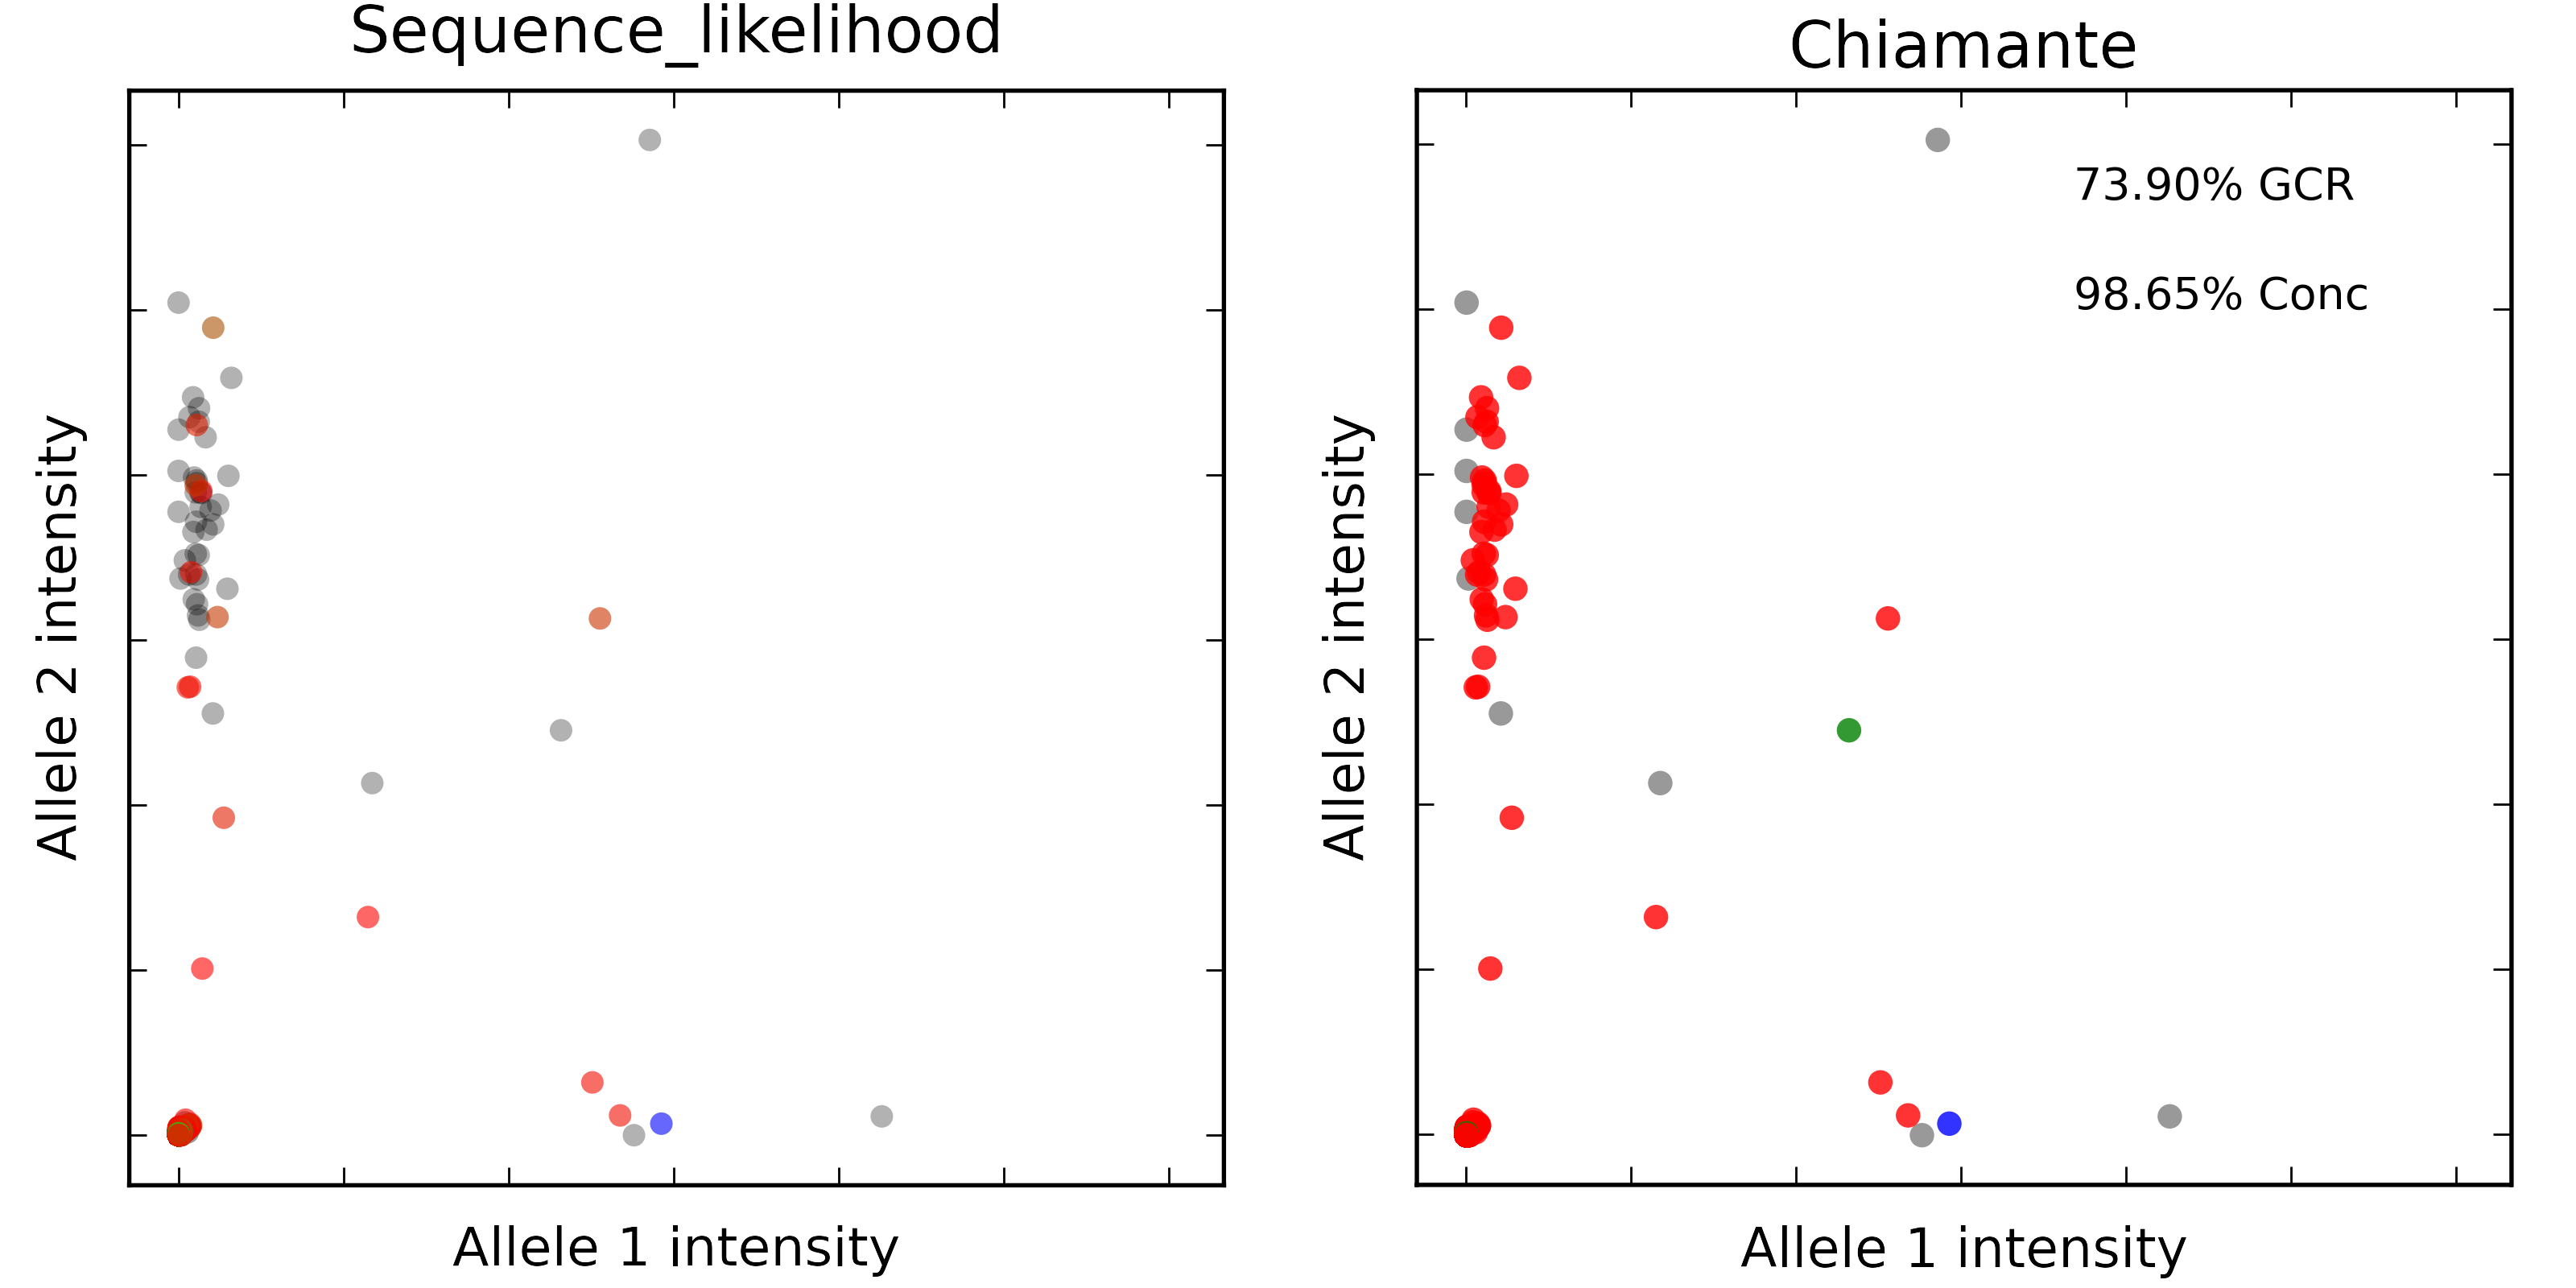
\includegraphics[width=\textwidth]{chap2figs/arrayfail_snp}
    \caption[Illustration of a SNP with high estimated array failure]{Illustration of a SNP with high estimated failure rate for the array assay ($\eta_X=0.71$). The left plot shows the cluster plot for the SNP with points coloured using a RGB colour scheme based on the scaled GLs for each genotype. The right hand plots shows the same cluster plot with points coloured according to the Chiamante posterior probabilities.   \label{array_fail_1}}
  \end{center} 
\end{figure}

\section{Discussion}

In this chapter we have introduced a genotype calling method for micro-array data that can leverage additional information from sequenced individuals and compared this model to other state of the art techniques.  As a traditional ``array only'' calling routine it is competitive with Illumina's proprietary software, achieving similar call rate and accuracy and substantially better that Illuminus and GenoSNP.  The addition of sequencing data makes our method the most accurate across a range of scenarios, although only by a modest margin.  This allows a greater number of SNPs (1000s) to pass standard QC filters.  The gains at low frequency sites were more substantial than common sites.  The failure indicators of the model also show potential as useful QC parameters.

An important limitation to note with this model is that it can identify when one of the assays has failed, but not both. Since we have reasonably realistic distribution for the failure mode of microarray data, observations that fit this failure distribution better than any of the genotype clusters can be flagged as uninformative and the sequence likelihoods are used.  However, sequence failures can only be identified when the GLs are strongly discordant with the information from microarrays. Hence in the case of very poor quality microarray data \emph{and} poor quality sequence data, the sequence data will not be flagged as erroneous.  In practice it would be prudent to filter SNPs where either assay has a high failure rate.

The model we have proposed may not capture the full complexity of imperfect sequence and array data. Our model assumes that assays have either succeeded or failed but they may include partial information. For example, errors in some reads covering a SNP site might contain sequencing errors or mapping errors that we do not model explicitly. To a certain extent the use of genotype likelihoods accounts for some of these error modes. Also, we have assumed errors are independent but errors could be correlated due to local sequence features such as GC content or proximity of SNPs to short insertions and deletions. 

Despite these limitations, the model performs well in general and even in the very extreme scenarios such as those shown in Figures~\ref{array_fail_1}~and~\ref{seq_fail_1}.  The gains we make are modest,  this is perhaps not surprising given that Illumina's standard software calls 99.72\% of genotypes with 99.71\% accuracy which is a testament to the high quality of the current generation of micro-array data.  Nevertheless, the computation required for our method is not substantial (< 1 day for the data set described here) and there is always a case for producing the most accurate set of genotypes as possible.





\chapter{Haplotype inference across the spectrum of relatedness}

\section{Background}
The estimation of haplotypes from SNP genotypes, commonly referred to as `phasing', is a well studied problem in statistical genetics. Existing approaches can be categorised according to the type of cohort each method is designed to phase, and the level of relatedness between the individuals in that cohort. Much of the recent literature is devoted to phasing so-called \emph{unrelated} individuals, such as cohorts that have been collected in many genome-wide association studies (GWAS). The term \emph{unrelated} used here is not strictly accurate, since the study individuals will share an evolutionary history. Individuals within such cohorts are usually distantly related, although it can be the case that cryptic relatives, which exhibit much closer relationships, can exist within these cohorts \citep{voight2005confounding}. Methods that have been developed for estimating haplotypes in such cohorts take advantage of linkage disequilibrium (LD). Over relatively short regions some individuals will share short stretches of sequence due to shared ancestry in that part of the genome. Another way to describe this is that individuals will share short stretches of sequence identical by descent (IBD). The most accurate methods use hidden Markov models (HMMs) that model local haplotype sharing between individuals \citep{stephens2001new, delaneau2013}.

Some of the methods designed for unrelated individuals can also handle mother-father-child trios and parent-child duos  \citep{marchini2006comparison, browning2009unified,delaneau2011linear,delaneau2013, williams2012phasing}. Phasing of such small families is relatively easy since the close family relationships place constraints on the underlying haplotypes, substantially reducing the amount of phase information that needs to be determined. Methods also exist for phasing more complex pedigrees, typically as part of more general pedigree analysis software \citep{lange2013mendel,sobel1996descent,abecasis2002merlin,gudbjartsson2000allegro}.  Whilst accurate, these methods are difficult to incorporate into pre-phasing and imputation pipelines that are now a standard part of genome-wide association studies and meta-analyses~\citep{howie2012fast}. 

The task of phasing in isolated populations is some what of a special case, as individuals from such populations exhibit much higher levels of relatedness. Isolated populations arise when a sub-population is isolated from the main population, which increases the degree of endogamy or within population marriage. This has the effect of reducing the effective population size, reduces genetic diversity and creates `long range' LD between sites in the genome. The reduced population size increases the chance that individuals share a very recent common ancestor, say between 1-10 generations ago. When comparing any two individuals from such populations we would expect to observe that they will share much longer stretches of sequence identically by descent (IBD) than a pair of unrelated individuals from a  non-isolated population.  These long IBD stretches can be exploited to infer very accurate haplotypes, an idea originally proposed by \cite{kong2008detection} who applied it to a large sample from the rather unique Icelandic population with high quality results.

A related problem to phasing is the detection of recombination events. Accurate detection of recombination events in a meiosis is important for the study of fine scale recombination, investigating the association between recombination rates and genetic variation, as well as other covariates and for the creation of genetic maps.  A duo or trio is usually insufficient to detect recombination events, as phasing with Mendel rules produces the haplotypes transmitted from the parent to the child, rather than the true parental haplotypes.  While this is sufficiently accurate for many applications, such as construction of haplotype reference sets~\citep{InternationalHapMapConsortium:2005cu} for imputation~\citep{marchini2010genotype}, it is clearly not useful for studying recombination.  

Recombination events can be inferred from a three generation pedigree since accurate phasing of both parents (via the grandparental genotypes) allows detection of recombination events in their children.  Alternatively, nuclear families with $>2$ children can be used to identify recombination events by examining differences in the transmitted haplotypes between siblings.  This was the approach used to create the deCODE family based map~\citep{kong2002} from families sampled from the Icelandic population, as well as by \cite{coop2008high} using individuals from a Hutterite population.  As genotyping error complicates such approaches, Coop applied ad-hoc filtering to detect clusters of unlikely recombination events and achieved good results.  Both of these studies exploit pedigrees that are informative about recombination.  In the absence of such data, we need to be able to very accurately phase the parental haplotypes using information from the wider population. This was recently achieved using a long-range phasing approach to obtain the true parental haplotypes (and hence recombination events) in Icelandic individuals~\citep{kong2010fine}.  

It would appear that different phasing tools (or a mixture thereof) should be applied depending on the demography of a cohort. In this chapter we give an overview of the popular methods for phasing cohorts of unrelated individuals, individuals that exhibit large tracts of IBD sharing (long range phasing) and the Lander-Green algorithm for extended pedigrees.  We also introduce our own technique for incorporating extended pedigree information into haplotypes that were inferred using methods for unrelated individuals, with the aim of overcoming the limitations of traditional pedigree approaches.  This method, called the duoHMM, ensures haplotypes are consistent with pedigree structure and can also detect recombination events. In chapter 4 we evaluate the accuracy of all of these approaches on real and simulated data. 

\subsection{The switch error metric}
Given a set of ``true'' validation haplotypes and some haplotypes inferred via a method, we require a sensible metric to evaluate the accuracy of each of our inferred haplotype sets.  Switch error (SE) rate was introduced by \cite{Lin:2002hh}  and has become the defacto metric for phasing evaluations~\citep{stephens2003comparison}.  It is defined as the proportion of adjacent heterozygote sites that are incorrectly aligned, each of these incorrect alignments is referred to as a switch error. We can think of this as the number of times an inferred haplotype needs to be switched (or flipped) so that it matches the true haplotype.  Figure~\ref{chap3:switcherror} (top) illustrates this idea showing an inferred haplotype which has two switch errors and six heterozygous sites resulting in a switch error rate of $\frac{2}{6-1}=0.4$

\begin{figure}[h]
  \begin{center} 
    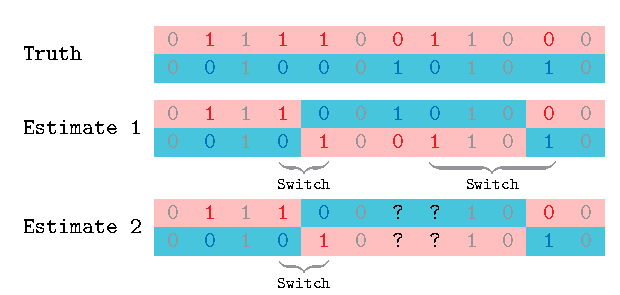
\includegraphics[width=\textwidth]{chap3figs/switcherror}
    \caption[Examples of the switch error metric]{Examples of the switch error metric.  The true underlying parental chromosomes are in pink and light blue with heterozygous sites (the sites of interest) highlighted in red and dark blue.   Estimate 1 has two switch errors present meaning that we would need to flip the estimated haplotype twice to arrive at the true underlying haplotype.  Estimate 2 is only partially phased (which can be the case with SLRP's output) and whilst there is a switch error between the heterozygous sites flanking the unphased region, we ignore this for comparison purposes since the algorithm was not attempting to align these sites correctly. \label{chap3:switcherror}}
  \end{center} 
\end{figure}
\clearpage
In this chapter we describe methods that are not capable of resolving every heterozygous site, the Lander-Green (LG) algorithm and SLRP, this complicates the evaluation of switch error rates. There are two types of missingness to consider here.  The first is where a heterozygous site is left unphased because that locus is heterozygous throughout a pedigree (LG) or throughout an IBD cluster (SLRP).  In this case the flanking heterozygote sites should still be aligned correctly if the method has not made an error and the IBD status has not changed.  We simply ignore such sites when calculating switch errors. The second case only occurs with SLRP's estimated haplotypes.  A chromosome may have large regions which are left completely unphased due to a lack of IBD sharing.  The flanking heterozygous sites of such a region will be phased at random, and we ignore switch errors in such cases essentially treating the phasing IBD blocks as mini-chromosomes. Figure~\ref{chap3:switcherror} (bottom) gives a toy example of two phased IBD chunks separated by an unphased region and how we calculate switch errors in such a situation.


\subsection{Statistical framework}
After genotype calling on microarrays similar to that described in the previous chapter, we are left with a vector of  genotypes at $L$ markers across a chromosome for individuals $i = 1...N$, that is $G_i = \{G_{i1},...,G_{iL}\}$.  We assume bi-allelic variants  so $G_{il}\in \{0,1,2\}$ is the sum of the two inherited parental alleles (coded as 0/1)  at the $l$th SNP.   Throughout this chapter, we denote the underlying pair of haplotypes (or diplotype) for an individual as $(h^1,h^2)$ where $h^1$ and $h^2$ are vectors of binary variables of length $L$ such that $G_{il} = h_{il}^1 + h_{il}^2$. Generally speaking, we typically wish to obtain the posterior distribution of an individual's haplotypes, conditional on their genotypes as well as other genotypes in a cohort (or within the same pedigree), that is $P(h^1,h^2|G_1,\ldots, G_N)$. All of the methods described in this chapter utilise HMMs of varying structure where the hidden states correspond to some relatedness between individuals in the cohort.  Depending on the sample this relatedness ranges from very distant (linkage disequilibrium) to very recent (explicit pedigree relationships).

\subsection{Hidden Markov Models}
Every model described in this chapter utilises some form of HMM to estimate haplotypes.  We briefly cover some key concepts  following the well known tutorial given by \cite{rabiner1989tutorial}.  Phasing applications typically involve discrete state Markov chains with inhomogeneous transition probabilities. We have a sequence of random states $Z=\{Z_1,\ldots,Z_L\}$ that follow the Markov property with transition probabilities that vary with position $l$. We do not observe these states directly, but rather some emitted variables, $X=\{X_1,\ldots,X_L\}$.  The distribution of $X_l$ depends on the hidden state $Z_l$. Hence we have two components for a HMM, the transition probabilities that describe the Markov process; $P(Z_1)$ and $P(Z_{l+1}|Z_l)$ as well as the conditional distribution of the observed variable $X$ given the state, $P(X|Z)$ (often referred to as the emission distribution).  The likelihood of some observed data is then
$$P(X) = \sum_Z P(Z_1) \prod_{i=2}^L P(Z_l|Z_{l-1}) \prod_{i=1}^L P(X_l|Z_l) $$
where we are summing over every possible state sequence $Z$.  Performing this calculation na\"{\i}vely is clearly intractable for any problem of moderate size, but can be found via a dynamic programming technique known as the Forward-Backward algorithm.  

The forward variable is defined as:
$$\alpha_l(k) = P(X_1,\ldots,X_l,Z_l=k)$$
which can be calculated by induction with initialisation step
$$\alpha_1(k) =   P(X_1|Z_1=k) P(Z_1=k)$$
and induction step 
$$\alpha_{l+1}(k) = P(X_{l+1}|Z_{l+1}=k) \sum_{k'=1}^K \alpha_l(k') P(Z_{l+1}=k|Z_l=k')$$
then $\sum_{k=1}^K \alpha_{L}(k)$ is the likelihood of the observed sequence.  Similarly we have the backward variable:
$$\beta_l(k) = P(X_{l+1},\ldots,X_L|Z_l=k)$$
which is calculated by induction with with initialisation step
$$\beta_L(k) = 1$$
and induction step 
$$\beta_l(k)  =  \sum_{k'=1}^K P(X_{l+1}|Z_{l+1}=k') \beta_{l+1}(k')P(Z_{l+1}=k'|Z_l=k)$$
Typically we are interested in the posterior distribution of the sequence $Z$ given the observed data $X$, that is $P(Z|X)$.  The forward and backward variables allow us to calculate the posterior probabilities of states at a specific location $l$:
$$P(Z_l=k|X_1,\ldots,X_L) \propto \alpha_l(k)\beta_l(k)$$
alternatively, we may be interested in the most likely state sequence rather than just the most likely state at one specific position.  The most likely state sequence can be found via the Viterbi algorithm which involves calculating the variable:
$$\delta_l(k) = \max_{k_1,\ldots,k_{l-1}} P(Z_1,\ldots,Z_l=k,X_1,\ldots,X_l)$$
which is the most likely state sequence leading up to state $k$ at time $l$.  This can be calculated recursively similarly to the forward variable with initialisation:
$$\delta_1(k) =   P(X_1|Z_1=k) P(Z_1=k)$$
and induction:
$$\delta_{l+1}(k) = P(X_{l+1}|Z_{l+1}=k) \max_{k'} \left(  \delta_l(k') P(Z_{l+1}=k|Z_l=k') \right)$$
in addition to $\delta$, we require the value of $k'$ that maximises this term for each $k$ and $l+1$.  Again using induction we have initialisation
$$\psi_1(k)=0$$
and induction step
$$\psi_l(k)=\argmax_{k'} \left(  \delta_l(k') P(Z_{l+1}=k|Z_l=k') \right).$$
We can then infer the most likely state sequence, $\{\hat{Z}_1,\ldots,\hat{Z}_L\}$ with initialisation
$$\hat{Z}_L = \argmax_{k}(\delta_T(k))$$
and induction
$$\hat{Z}_l = \psi_{l+1}( \hat{Z}_{l+1})).$$
Rather than obtain the most likely state sequence, we may wish to sample a state sequence from the distribution $P(Z_1,\ldots,Z_L|X)$.  This is an effective way of taking into account the uncertainty in the estimated sequence and is of use in the Markov Chain Monte Carlo (MCMC) routines described later in this chapter. To sample a sequence, we only require the calculation of the forward variable.  We first sample a state at position $L$ from 
$$P(\hat{Z}_L=k|X)  \propto \alpha_L(k)$$
and then recurse backwards sampling at each $l$:
$$P(\hat{Z}_l=k|\hat{Z}_{l+1}=k',X) \propto \alpha_l(k) P(\hat{Z}_l=k|\hat{Z}_{l+1}=k')$$
terminating at $l=1$.  

It is important to note that the complexity of calculating the forward, backward and Viterbi variables is $O(LK^2)$.  This means computation will scale well with the number of markers (which can be very large in phasing applications) but will rapidly become intractable as the state space increases. Many of the advances in phasing described in this chapter involve innovative ways of reducing the state space whilst maintaining accuracy.


\section{Methods for nominally unrelated individuals}
\label{chap3:unrelated}
\subsection{The Li and Stephens Model for Linkage Disequilibrium}
\label{chap3:liandstephens}
The Li and Stephens model~\citep{li2003model} is now a classic approximate model for linkage disequilibrium that was originally proposed to perform inference on recombination rates across a chromosome.  It forms the basis for various phasing (and associated imputation) software such as IMPUTE1~\citep{marchini2007new}, IMPUTE2~\citep{howie2009flexible}, MaCH~\citep{li2010mach}, HAPI-UR~\citep{williams2012phasing} and both versions of SHAPEIT~\citep{delaneau2013,delaneau2011linear}.

Consider the case where we have $K$ known haplotypes sampled from the population, $H =\{H_1 \ldots H_K\}$ where $H_k=\{H_{k1},\ldots,H_{kL}\}$.  The $K+1$ sampled haplotype, $h=\{h_1,\ldots,h_L\}$, is modelled as a mosaic of the $K$ already sampled haplotypes, along with some sporadic allelic differences due to mutation events. Put another way, haplotype $h$ ``copies from'' different haplotypes in the sample at different regions along the chromosome. We use $Z_l \in \{1,\ldots,K\}$  to denote which of the $K$ haplotypes is being copied from at position $l$.  This forms a Hidden Markov Model with transition probabilities varying according to recombination rates where $h$ is the observed variable and $Z$ are the hidden states of the chain. The initial state is distributed uniformly:
$$P(Z_1=k) = 1/K$$
at subsequent markers, state transitions are
\[ P(Z_{l+1}=k|Z_l=k')  = \left\{ 
  \begin{array}{l l}
    \frac{1-\exp(-\frac{\rho_l}{K})}{K} & \quad k \neq k'\\
    \exp(-\frac{\rho_l}{K}) + \frac{1-\exp(-\frac{\rho_l}{K})}{K} & \quad k = k'
  \end{array}  \label{chap3:listephentrans}
  \right.\]
where $\rho_l = 4N_er_l$ and $r_l$ is the genetic distance (in Morgans) between sites $l$ and $l+1$. This transition matrix has two intuitively sensible properties. First, when the distance between markers is small, then those markers are highly likely to copy the same chromosome. Second, as the sample size $K$ increases, the chance of a change in copying state decreases, meaning longer haplotype chunks tend to me copied.

Mutation events are handled by the emission distribution:
\begin{equation}
%\[ 
P(h_l= A_{kl}|Z_l=k) = \left\{ 
  \begin{array}{l l}
    1-\frac{\theta}{2(\theta+K)}               & \quad h_l = A_{kl}  \\
    \frac{\theta}{2(\theta+K)}      & \quad h_l \neq A_{kl} 
  \end{array}  
\right.
%\]
\label{chap3:listephenmut}
\end{equation}
where $A_{kl}$ denotes the allele carried by the $k$th haplotype at site $l$. The parameter  $\theta = (\sum_{m=1}^{K-1} \frac{1}{m})^{-1}$ controls the rate of mutation.  The intuition behind this choice of $\theta$ is that $\theta \times (\sum_{m=1}^{K-1} \frac{1}{m})$ is the expected number of mutations events at a single site for $K$ individuals, the model sets this expectation to 1 and solves for $\theta$.

The Li and Stephens model has the desirable property that the length and fidelity of haplotypes copied increases with $K$, reflecting the fact that as sample size increases, individuals will tend to share larger and more similar haplotypes. It also has the crucial benefit of allowing tractable inference using well developed HMM inference machinery.

\subsubsection{Inference with the Li and Stephens Model}
The likelihood for an individual haplotype is
$$P(h_1,\ldots, h_L|H) = \sum_Z \prod_{l=1}^L P(h_l|Z_l) P(Z_1) \prod_{l=2}^L  P(Z_l|Z_{l-1})$$
here we need to integrate over every possible configuration of copying sequences ($Z$), which is a standard operation for HMMs using the Forward-Backward algorithm. Whilst in general inference on a HMM with $K$ states will have computational cost of  
$O(LK^2)$, inference on the Li and Stephens model can be performed in $O(LK)$ due to the probability of a change in copying state being the same regardless of which states are being transitioned between.  For example if we take the standard HMM forward variable:
$$\alpha_l(k) = P(h_1,\ldots,h_l,Z_l=k)$$
which is calculated by induction with initialisation step
$$\alpha_1(k) = \frac{1}{K} P(h_1|Z_1=k)$$
and induction step 
\begin{eqnarray*}
\alpha_{l+1}(k) & = & P(h_{l+1}|Z_{l+1}=k) \sum_{k'=1}^K \alpha_l(k')P(Z_{l+1}=k|Z_l=k') \\
					&=& P(h_{l+1}|Z_{l+1}=k)\left( \exp(-\frac{\rho_l}{K})\alpha_l(k) + \frac{1-\exp(-\frac{\rho_l}{K})}{K}\sum_{k'=1}^K\alpha_l(k')\right)
\end{eqnarray*}
the right term of the summation is the same for all $k$ and hence only needs to be evaluated once per site so computation scales with $O(LK)$ complexity.  For the same reason, calculation of the backward variable and the Viterbi algorithm are both $O(LK)$. Hence the Li and Stephens model offers a powerful tool for the tractable analysis of genetic data where both the sample size $K$ and number of sites $L$ can be very large.

%% Similarly for the backward variable:
%% $$\beta_l(k) = P(h_{l+1},\ldots,h_l|Z_l=k,\rho)$$
%% which is calculated by induction with with intialisation step
%% $$\beta_L(k) = 1$$
%% and induction step 
%% \begin{eqnarray*}
%% \beta_l(k) & = & \sum_{k'=1}^K P(h_{l+1}|Z_{l+1}=k') \beta_{l+1}(k')P(Z_{l+1}=k'|Z_l=k) \\
%% &=&  \frac{1-\exp(\frac{\rho_l}{K})}{K}\sum_{k'=1}^KP(h_{l+1}|Z_{l+1}=k')\beta_{l+1}(k') + \exp(-\frac{\rho_l}{K})P(h_{l+1}|Z_{l+1}=k)\beta_{l+1}(k)
%% \end{eqnarray*}
%% Again we can save computation  by only computing the left term of the summation once. Inference on HMMs revolves around these two calculations as well as the Viterbi algorithm (which is similar to the forward variable calculation) 


\subsection{Phasing with the Li and Stephens Model}
\label{chap3:LSphase}
The previous section gave us a useful model for observed \emph{haplotypes} in a sample, but in practice we observe \emph{genotypes}. IMPUTE1 and IMPUTE2 extended the Li and Stephens model to genotype data for the purposes of phasing and genotype imputation from haplotype reference panels (a closely related problem).  We summarise the general approach of this extension here.


\begin{figure}[h]
  \begin{center} 
    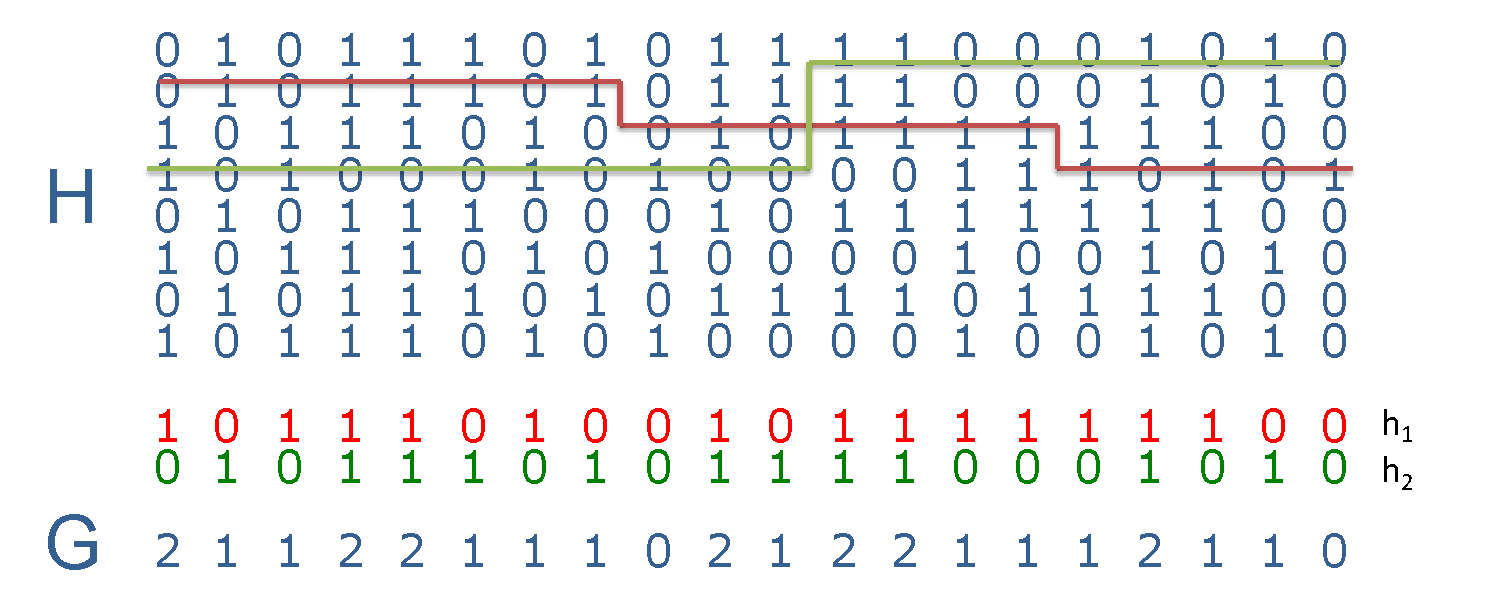
\includegraphics[width=\textwidth]{chap3figs/haplotype_path}
    \caption[Inferring haplotypes with the Li and Stephens Model]{An example of a pair of copying paths for the diploid Li and Stephens model used to infer an individual's underlying haplotypes, $(h_1,h_2)$, from that individual's genotype data $G$.  The individual's haplotypes are inferred as a mosaic of other \emph{conditioning haplotypes}, $H$ in the population.   \label{chap3:happath}}
  \end{center} 
\end{figure}

Given a set of conditioning haplotypes, $H$, an individual's diplotype, $(h^1,h^2)$, originates from a pair of sequences of hidden states $(Z^1,Z^2)$ where $(Z^1_l,Z^2_l)\in\{1\ldots K\}$ denote which conditioning haplotypes  an individual's haplotype  pair is copying from at site $l$.  Using the model defined in the previous section and assuming an individual's haplotypes are independent of one another, we now have a Hidden Markov Model with $K^2$ states (every possible pairing of copying states). 

The initial state probabilities for Markov chain are:
$$P(Z_1^1=k_1,Z_1^2=k_2) = 1/K^2$$
and the transition probabilities are:
\small
\[ P(Z_{l+1}^1=k_1,Z_{l+1}^2=k_2 | Z_l^1=k_1',Z_l^2=k_2') = \left\{ 
  \begin{array}{l l}
    \left( \exp(-\frac{\rho_l}{K}) + \frac{1-\exp(-\frac{\rho_l}{K})}{K} \right) ^2 & \quad k_1=k_1',~k_2=k_2'\\
    \left( \frac{1-\exp(-\frac{\rho_l}{K})}{K} \right) \left( \exp(-\frac{\rho_l}{K}) + \frac{1-\exp(-\frac{\rho_l}{K})}{K} \right) & \quad k_1 \neq k_1' \oplus  k_2 \neq k_2'\\
    \left( \frac{1-\exp(-\frac{\rho_l}{K})}{K} \right)^2 & \quad k_1\neq k_1',~k_2\neq k_2'\\
  \end{array} \right.\label{chap3:jump}\] 
\normalsize
these probabilities correspond to 0, 1 and 2 ``jumps'' between which conditioning haplotypes an individual's diplotype is copying from. Figure~\ref{chap3:happath} provides an example of a genotype and corresponding paths through the conditioning haplotypes. 

 Given an observed genotype $G_{il}$ at position $l$ and hidden states $(Z^1_l,Z^2_l)$, the emission distribution $P(G_{il}|Z^1_l,Z^2_l)$ for each possible combination is: 
\vspace{10pt}
\begin{center}
\begin{tabular}{|c|l|cccc|}
  \hline
  &  &\multicolumn{4}{c|}{$G_{il}$}\\
  &  & 0 & 1 & 2 & Missing \\ 
  \hline
  \multirow{3}{*}{$h_{Z^1_l}+h_{Z^2_l}$} & 0 & $(1-\lambda)^2$ & $2\lambda(1-\lambda)$ & $\lambda^2$ & 1.0 \\ 
                                     & 1 & $2\lambda(1-\lambda)$ & $\lambda^2 + (1-\lambda)^2$ & $2\lambda(1-\lambda)$  & 1.0 \\ 
                                     & 2 & $\lambda^2$ &$2\lambda(1-\lambda)$ &$(1-\lambda)^2$ & 1.0 \\
   \hline
\end{tabular}
\end{center}
\vspace{10pt}
where $\lambda=\frac{\theta}{2(\theta+K)}$, the mutation probability seen in the Li and Stephens model (Equation~\ref{chap3:listephenmut}). Note that this model easily accommodates missing genotypes by placing a flat likelihood across also possible genotype values. The likelihood for an observed genotype vector is then
\begin{equation}
P(G_i|H) = \sum_{Z^1,Z^2} ~\prod_{l=1}^L  P(Z_{l}^1,Z_{l}^2) \prod_{l=1}^L P(G_{il}|Z^1_l,Z^2_l).
\label{chap3:impute2lik}
\end{equation}
here we are summing over all possible unobserved paths ($Z_1,Z_2$). 

 We are primarily interested in the posterior distribution of an individual's haplotypes conditional on all other information, $P(h_1,h_2|G_i,H)$ which in turn is determined by the pair of copying paths $P(Z_1,Z_2|G_i,H)$. The complexity of our state space has increased substantially compared to the haploid model described previously.  Consider the calculation for the forward variable of this model:
$$\alpha_l(k_1,k_2) = P(G_{i1}\ldots G_{il+1},Z_{l+1}^1=k_1,Z_{l+1}^2=k_2|H)$$
with initialisation step:
$$\alpha_1(k_1,k_2) = \frac{1}{K^2} \times (G_{il}|Z^1_l=k_1,Z^2_l=k_2)$$
and induction step:
\begin{eqnarray*}
  \alpha_{l+1}(k_1,k_2) & = & P(G_{il}|Z^1_l=k_1,Z^2_l=k_2) \times\\
  &&\Bigg[  \left(\exp(-\frac{\rho_l}{K}) + \frac{1-\exp(-\frac{\rho_l}{K})}{K}\right)^2 \alpha_l(k_1,k_2)\\
    && + \left( \frac{1-\exp(-\frac{\rho_l}{K})}{K} \right) \left( \exp(-\frac{\rho_l}{K}) + \frac{1-\exp(-\frac{\rho_l}{K})}{K} \right) \left( \sum_{k'=1}^K \alpha_l(k',k_2) + \sum_{k'=1}^K \alpha_l(k_1,k')\right)\\
    && +  \left( \frac{1-\exp(-\frac{\rho_l}{K})}{K} \right)^2 \left( \sum_{k_1'=1}^K \sum_{k_2'=1}^K \alpha_l(k_1',k_2') \right) \Bigg]
\end{eqnarray*}
the middle summations require $2K^2$ operations to calculate across all pairs of $(k_1,k_2$). \cite{scheet2006fast} provide derivations which exploit the symmetry $ \alpha_{l}(k_1,k_2) =  \alpha_{l}(k_2,k_1)$ to avoid redundant computations, approximately halving the computational burden. This is an important implementational detail but we exclude it for clarity. The essential point is that inference procedures for HMMs on genotype data under the Li and Stephens model now scale quadratically with the size of $H$.

We have described the model assuming that conditioning haplotypes were known, we could possibly use a reference panel of haplotypes such as those available from the 1000 Genomes Project, which was in fact how IMPUTE1 functioned.  However results from the development of IMPUTE2 showed that phasing using in-sample conditioning haplotypes was more effective than the reference panel only approach. Hence using conditioning haplotypes present in the sample is preferable, but of course these are unknown, so we need to integrate over this uncertainty. This can be achieved via an MCMC approach.

Given a sample of $N$ genotyped individuals, $G = G_1\ldots G_N$, we wish to infer each individual's diplotypes ($2N$ haplotypes), $H = \{H_1,\ldots,H_{2N}\}$.  We can initialise the haplotypes of all individuals by randomly assigning phase at all heterozygous sites.  We can then iterate over each individual, sampling a diplotype from $P(h^1,h^2|G_i,H \setminus (H_{2i-1},H_{2i}))$.  This process is repeated for a set number of iterations.  Finally we can either run the Viterbi algorithm to find the most likely haplotypes for an individual or take the most likely diplotype per site $l$. An issue with this approach is that computation scales quadratically with sample size $N$ meaning the method rapidly becomes intractable with increasing sample size.  This problem can be circumvented by only conditioning on a subset of size $K<2(N-1)$ of the haplotypes in the sample, constraining computation to $O(LK^2)$.

\subsubsection{Choosing conditioning haplotypes}
We could choose these $K$ conditioning haplotypes at random from the cohort which is the approach used by MaCH.  Alternatively, we could try to choose conditioning haplotypes such that they are likely to be ``copied'' from by the individual being phased. This is the ``surrogate-family'' approach introduced by IMPUTE2. In this approach, the Hamming distance between the individual's previously sampled haplotypes $H_i=(h^1_i,h^2_i)$ and all other $2(N-1)$ haplotypes present in the sample is calculated. The Hamming distance is simply the sum of alleles that are different across a region.  The $K$ haplotypes with the smallest distance measures, $H^{*}=\{H_1,\ldots,H_K\}$, are used as the conditioning set for individual $i$.  We then work with the posterior $P(h_1,h_2|G_i,H^{*})$  which restrains the HMM computations to $O(K^2L)$ complexity. Since an individual's closest ancestors in a sample will vary across a chromosome, it was recommended to run IMPUTE2 on chunks of several Mb so that a different $H^{*}$ would be used in different genomic regions.

This can be thought of as conditioning on all haplotypes in the cohort in a very crude manner, as all haplotypes are still being compared.  Since the distance calculations involve comparing each individual to all $N$ samples in a cohort at all loci, they have $O(N^2L)$ complexity.  However because these operations are very rapid, the HMM calculations dominate computation for $N<10000$.  As sample sizes increase to tens of thousands of individuals, these distance calculations begin to comprise the majority of computation. 

\subsection{The SHAPEIT2 approach}
The Segmented HAPlotype Estimation and Imputation Tool version 2 (SHAPEIT2)~\citep{delaneau2013} is a recently developed method for phasing unrelated individuals. It combines a novel data structure for efficiently representing the space of possible  haplotypes of an individual which was introduced in the original SHAPEIT1~\citep{delaneau2011linear} along with the ``surrogate-family'' conditioning haplotype selection idea introduced by IMPUTE2. The main advantage of this approach over IMPUTE2 is that the HMM calculations  scale \emph{linearly} with the number of conditioning haplotypes, this means computation can performed tractably with larger values of $K$ leading to greater accuracy and less computation time.

An individual's genotype vector $G_i$ can be partitioned into $C$ segments where each segment contains $B$ heterozygous sites.  There will be $2^B$ consistent haplotypes within each of these segments.  The vector $S_l \in \{1\ldots C\}$ denotes which segment contains locus $l$. A haplotype that is consistent with $G_i$ across the chromosome can now be represented as a sequence of labels $X = \{x_1,\ldots,x_L\}$  where $x_l$ is now the label of the segmental haplotype at position $l$.  We allow the label $X$ to change only between segments, that is, when $S_l\neq S_{l+1}$.  Figure~\ref{chap3:s2seg} shows an example of this graph for three segments and $B=2$. A sequence $X$ now uniquely defines a haplotype that is consistent with $G$. 

Furthermore, the sequence $X$ also implies its unique complementary haplotype (to enforce consistent genotypes with $G$), so $X$ in fact implies a diplotype consistent with $G$.  This is the key to SHAPEIT2's linear complexity calculations, inference is now being performed on one haploid path, $X$, rather than a pair of haploid paths as in IMPUTE2.

\begin{figure}
  \begin{center} 
    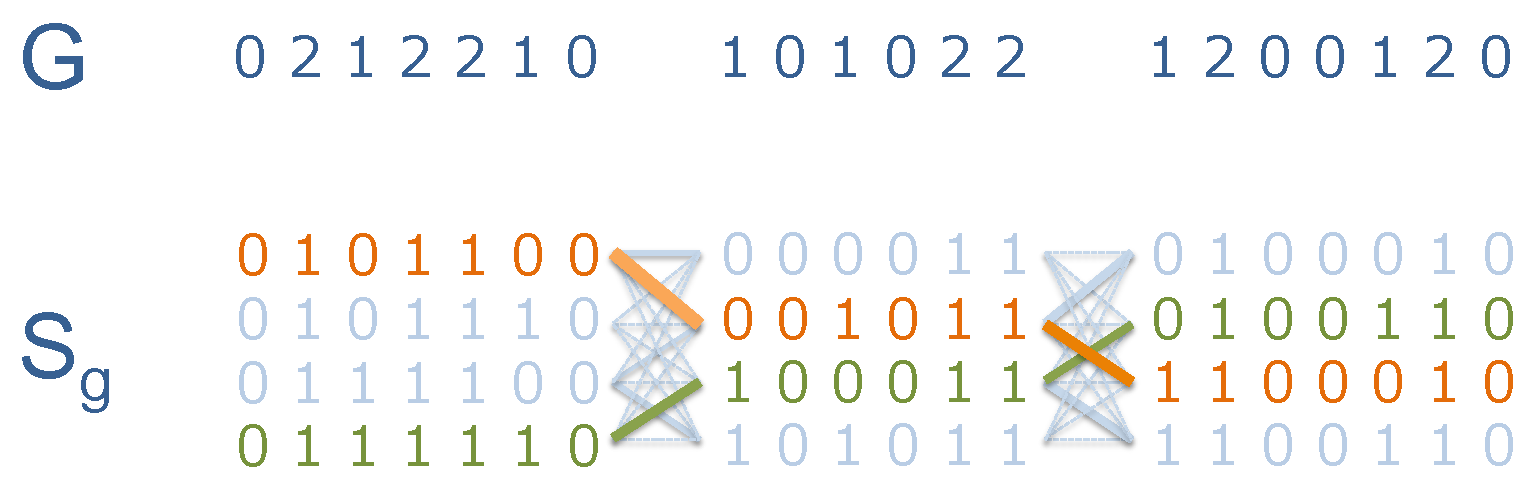
\includegraphics[width=\textwidth]{chap3figs/shapeit_model}
    \caption[The SHAPEIT2 diploid model]{The SHAPEIT2 diploid model, within each segment containing $B=2$ two heterozygous genotypes there are $2^B$ possible haplotypes.  Transitions between different haplotype labels are only possible \emph{between} segments, not within them.  The green and orange colouring labels a pair of paths consistent with the genotype vector.\label{chap3:s2seg}}
  \end{center} 
\end{figure}

This segmentation provides a graph that captures every possible haplotype for an individual, we can weight the edges of this graph using patterns of LD present in the conditioning haplotypes $H$ and the Li and Stephens model. This introduces a second latent variable $Z$,  denoting the haplotype in $H$ being copied from. For a single consistent haplotype, there are now two unobserved sequences, $X$ and $Z$.  Hence we perform inference on the likelihood:

$$P(X,Z|H) = P(X_1|Z_1,H) P(Z_1) \prod_{l=2}^L P(X_l,Z_l|X_{l-1},Z_{l-1},H)$$

We take the same transition probabilities as used in the haploid Li and Stephens model, but with the added restriction that the haplotype label ($X_l$) can only change when positions $l$ and $l-1$ are on different segments.  So when $S_l=S_{l-1}$ then transition probabilities are
\[ P(X_l=i,Z_l=k|X_{l-1}=j,Z_{l-1}=k',H) = \left\{ 
  \begin{array}{l l}
%     P(X_l=i,Z_l=k,H) P(Z_l=k|Z_{l-1}=k')  & \quad i=j\\
    P(Z_l=k|Z_{l-1}=k')  & \quad i=j\\
     0    & \quad  i\neq j\\
  \end{array} \right.\] \label{chap3:listephentrans} 
and when sites are on different segments ($S_l\neq S_{l-1}$) any transition is possible so
%$$ p(X_l=i,Z_l=k|X_{l-1}=j,Z_{l-1}=k',H) =  P(X_l=i,Z_l=k,H) P(Z_l=k|Z_{l-1}=k') $$
$$ p(X_l=i,Z_l=k|X_{l-1}=j,Z_{l-1}=k',H) =  P(Z_l=k|Z_{l-1}=k') $$
The emission probability is also the same as the Li and Stephens mutation model (Equation~\ref{chap3:listephenmut}):
\[ P(X_l=i|Z_l=k,H)  = \left\{ 
  \begin{array}{l l}
    \frac{\theta}{2(\theta+K)}               & \quad H_{kl} \neq A_{il}\\
    1-\frac{\theta}{2(\theta+K)}      & \quad H_{kl} = A_{il}
  \end{array}  
\right.\]
where $A_{il}$ is the allele carried by the $i$th haplotype segment at position $l$.  

SHAPEIT2 then applies a custom Forward-Backward algorithm to calculate the marginal distribution of $X$ with respect to hidden sequence $Z$.  This calculation is linear with respect to the size of $H$.  The forward variable in this case is 
$$\alpha_l(i,k) = P(X_l=i,Z_l=k,G_1,\ldots,G_l|H)$$
with initialisation:
$$\alpha_1(i,k) = P(X_1=i|Z_1=k)P(Z_1=k)$$
and induction step:
$$\alpha_{l+1}(i,k) =  \sum_{j=1}^{2^B} \sum_{k'=1}^K \alpha_l(j,k') P(X_{l+1}=i,Z_{l+1}=k|X_l=j,Z_l=k')$$
because the transitions probabilities vary according to whether $l+1$ and $l$ are in the same segment we need to consider two cases for the forward variable. When $S_l=S_{l+1}$  we only need to consider transitions where $i=j$ so:
\begin{eqnarray*}
  \alpha_{l+1}(i,k) &=& \sum_{k'=1}^K   \alpha_l(i,k') P(X_l=i,Z_l=k,G_1,\ldots,G_l|H)\\
  &=& P(X_{l+1}=i|Z_{l+1}=k,H) \left(\exp(-\frac{\rho_l}{K})\alpha_l(i,k) + \frac{1-\exp(-\frac{\rho_l}{K})}{K}\sum_{k'=1}^K \alpha_l(i,k')  \right)\\
\end{eqnarray*}note the term $\sum_{k'=1}^K \alpha_l(i,k')$ only needs to be computed once per $k$. When $S_l\neq S_{l+1}$  any segment transition is possible so:
\begin{eqnarray*}
\alpha_{l+1}(i,k) &=&  \sum_{j=1}^{2^B} \sum_{k'=1}^K \alpha_l(j,k') P(X_{l+1}=i,Z_{l+1}=k|X_l=j,Z_l=k')\\
&=& P(X_{l+1}=i|Z_{l+1}=k)\left(\exp(-\frac{\rho_l}{K}) \sum_{j=1}^{2^B} \alpha_l(j,k) + \frac{1-\exp(-\frac{\rho_l}{K})}{K} \sum_{j=1}^{2^B} \sum_{k'=1}^K \alpha_l(j,k') \right)\\
\end{eqnarray*}the terms $\sum_{k'=1}^{K} \alpha_l(i,k')$ and $\sum_{j=1}^{2^B} \sum_{k'=1}^K \alpha_l(j,k')$ only need to be computed once per $i$ and $l$ respectively. Hence the complexity of the forward variable calculations is only $O(KL)$, this is the primary advantage of introducing the intermediate latent variable $X$.  

By similar derivations we have a linear complexity calculation for the backward variable as well. Initialisation:
$$\beta_L(i,k)=1$$
and induction:
  \[ \beta_l(i,k) = \left\{ 
  \begin{array}{l ll}
   & e^{-\frac{\rho_l}{K}}\beta_{l+1}(i,k) P(X_{l+1}=i|Z_{l+1}=k)& \\ &~~~~~+ \frac{1-e^{-\frac{\rho_l}{K}}}{K} \sum_{k'=1}^K \beta_{l+1}(i,k')P(X_{l+1}=i|Z_{l+1}=k')   & \quad S_l=S_{l+1}\\
    &e^{-\frac{\rho_l}{K}} \sum_{j=1}^{2^B} \beta_{l+1}(j,k) P(X_{l+1}=j|Z_{l+1}=k)& \\ &~~~~~+ \frac{1-e^{-\frac{\rho_l}{K}}}{K} \sum_{j=1}^{2^B} \sum_{k'=1}^K \beta_{l+1}(j,k')P(X_{l+1}=j|Z_{l+1}=k)  & \quad S_l \neq S_{l+1} \\
  \end{array}  
  \right.\]
Once we have the forward and backward variables, we can take the marginal distribution of $X$ with respect to $Z$ and work with the posterior distribution $P(X|H)$. Since there are only $2^B$ states, inference on the segmented graph is very rapid.  We can obtain marginal distribution of being in a certain state $i$ at position $l$ from
$$P(X_l=i|H) \propto \sum^K_{k=1}\alpha_l(i,k)\beta_l(i,k)$$
and the transition probabilities at each site $l$:
\small
\begin{eqnarray*}
  P(X_l=i|X_{l+1}=j,H)& \propto& \sum_{k_1}\sum_{k_2} \alpha_l(i,k_1)P(Z_{l+1}=k_2|Z_l=k_1)P(X_{l+1}=j|Z_{l+1}=k_2)\beta_{l+1}(j,k_2)\\
  & \propto& \sum_{k_1}  \alpha_l(i,k_1) \sum_{k_2}P(Z_{l+1}=k_2|Z_l=k_1)P(X_{l+1}=j|Z_{l+1}=k_2)\beta_{l+1}(j,k_2)\\
  & \propto& \sum_{k_1} \alpha_l(i,k_1) \Bigg( \exp(-\frac{\rho_l}{K})P(X_{l+1}=j|Z_{l+1}=k_1)\beta_{l+1}(j,k_1)\\
  &&~~~~~~~~~~~~~~~~~ + \frac{1-\exp(-\frac{\rho_l}{K})}{K} \sum_{k_2}P(X_{l+1}=j|Z_{l+1}=k_2)\beta_{l+1}(j,k_2) \Bigg)
\end{eqnarray*}
\normalsize
Since the term $\sum_{k_2}P(X_{l+1}=j|Z_{l+1}=k_2)\beta_{l+1}(j,k_2)$ does not depend on $k_1$ it can be pre-computed (per $i,j$) and so this calculation is linear with $K$.  Hence SHAPEIT2 can find the posterior distribution of $X$ in linear time with respect to $K$, this provides a powerful new way of performing inference using the Li and Stephens model in the diploid setting.  

The calculation of the marginal transition probabilities (and the marginal state probability at $l=1$) for $Z$ allow us to simulate consistent haplotypes directly from the diploid graph which is a very quick operation. Similar to IMPUTE2, SHAPEIT2 performs an MCMC updating scheme to integrate over the uncertainty in haplotypes in a sample. It performs this for a fixed number of burn-in iterations, then performs a number of pruning operations where unlikely segment transitions are given a probability of 0 (removed from the graph), finally a number of sampling iterations are performed to average over the transition probabilities just described.  SHAPEIT2 then finds the most likely haplotype pairs for individuals by performing the Viterbi algorithm on its segmented graph. 

 Conditioning haplotypes are selected based on minimum Hamming distance as described previously for IMPUTE2.  SHAPEIT2 uses $K=100$ conditioning haplotypes by default and divides a chromosome up into windows (default 2Mb) choosing a different $H^{*}$ in each of these windows. The HMM calculations dominate computation for SHAPEIT2 up to $N\approx10000$, for larger sample sizes the quadratic cost of the distance calculations becomes a substantial portion of compute time. We discuss further modifications to the algorithm to circumvent the quadratic cost for $N>>10000$ in chapter 5. 

\subsection{Beagle}
The methods described so far have relied on a model for linkage disequilibrium based on an approximation to the coalescent.  Beagle takes a different approach in that it determines patterns of LD from the data using a variable length Markov chain (VLMC) to create a ``localised haplotype-cluster model''.  Given a set of haplotypes $H$, Beagle builds a directed acyclic graph with $L+1$ levels.  Where edges of the graph correspond to alleles and vertices correspond to the configurations of two adjacent alleles. Every haplotype in $H$ can be represented by a path through this graph.  A realisation of this model for some toy data is presented in Figure~\ref{chap3:beaglefig}, this is the example given in the original Beagle phasing paper~\citep{browning2007}.

The edges of this graph are weighted according to the frequencies with which haplotypes pass through them. If we consider the edges at each level (position) of the graph to be states of a Markov chain we can calculate transition probabilities from these weights.  Then the transition probabilities for leaving state $i$ at position $l$ and entering state $j$ at positions $l+1$  are easily calculated as the proportion of haplotypes using edge $j$ that leave the vertex edge $i$ enters, if edge $i$ has a different child vertex to $j$'s parent then the probability is 0.  For example, haplotypes 0000, 0001, 1000 and 1001 (237 total) pass through edge $e_F$ and haplotypes 0011 and 1011 pass through $e_G$ (247 total) giving us  $P(e_F|e_C) = P(e_F|e_D) = \frac{237}{237+247} = 0.49$ and $P(e_F|e_E)=0$ since $e_E$'s child is not $e_F$'s parent. This Markov process is the basis of Beagle's phasing routine.

\begin{figure}

  \begin{minipage}[t]{0.25\textwidth}
    \vspace{30pt}
%\vfill
    \begin{tabular}{lr}
      \hline
      Haplotype & Count \\
      \hline
      0000&	21\\
      0001&	79\\
      0011&	95\\
      0110&	116\\
      1000&	25\\
      1001&	112\\
      1011&	152\\
      \hline
    \end{tabular}
%\vfill
  \end{minipage}
  \hfill
  \begin{minipage}[t]{0.7\textwidth}
    \vspace{0pt}
    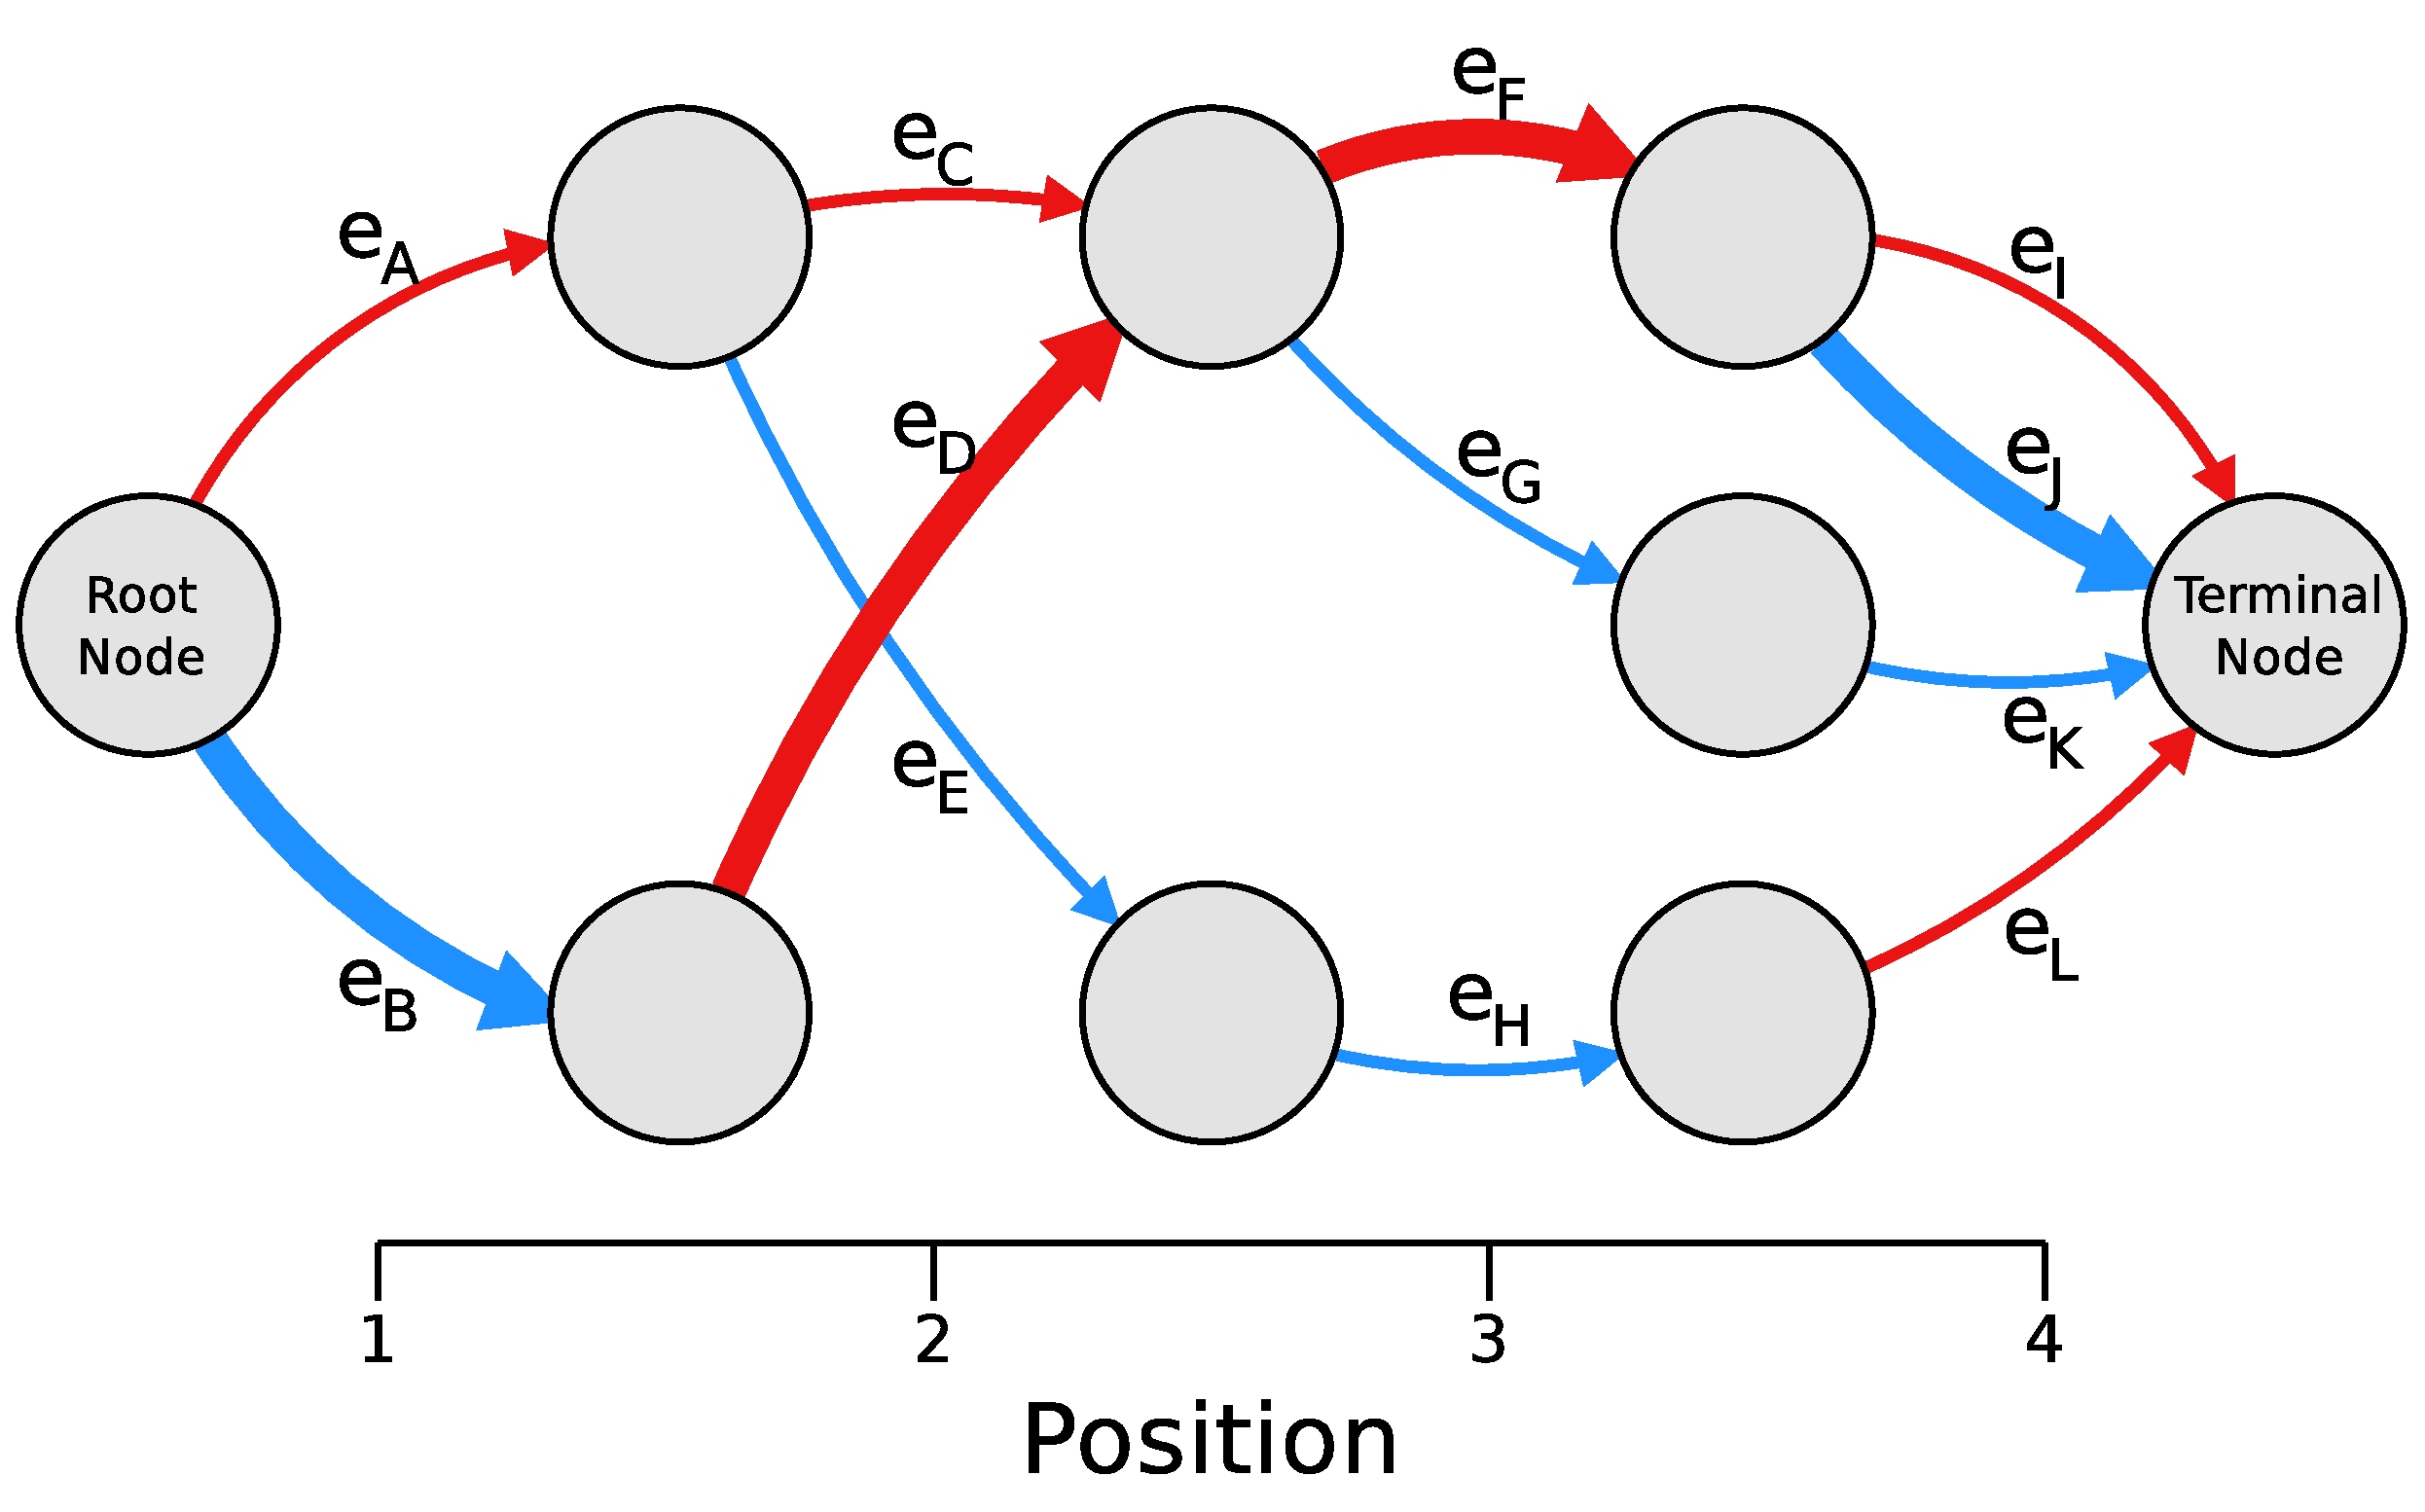
\includegraphics[width=\textwidth]{chap3figs/beagle}
  \end{minipage}
  \caption[The Beagle haplotype model]{\textbf{Left:} Observed haplotypes across four sites. \textbf{Right:} The Beagle haplotype cluster graph that represents these haplotypes. Red edges correspond to the 0 allele and blue correspond to the 1 allele. Each path from the root to terminal node is a haplotype listed in the table. The bold edges denote the path representing the 1001 haplotype.\label{chap3:beaglefig}}
\end{figure}

Beagle initialises all individuals' haplotypes by assigning random phase to heterozygous sites.  It then builds its haplotype graph and calculates the forward variable for each individual, which can then be used to sample a consistent haplotype pair for each individual. The haplotype graph is then rebuilt from these newly sampled haplotypes.  On the final pass the Viterbi algorithm is applied rather than path sampling to obtain final haplotype estimates.  Perhaps the most impressive aspect of Beagle is the speed with which the model converges, ten iterations are used by default and increasing this number yields little improvement in accuracy~\citep{browning2007}.  Whilst the Beagle graph greatly reduces the state space of the HMM, the construction of the graph is somewhat computationally expensive with cost somewhere between linear and quadratic time.  This will limit Beagle's utility for very large samples.
\subsection{HAPI-UR}
The \textbf{HAP}lotype \textbf{I}nfer-ence for \textbf{U}n\textbf{R}elated samples (HAPI-UR)~\citep{williams2012phasing} method is a relatively new phasing method developed with very large samples in mind.  Similar to Beagle and SHAPEIT1 it collapses conditioning haplotypes $H$ into a graph structure which is then used to infer haplotype pairs per individual. The difference between Beagle and HAPI-UR is that the states that this graph represents are no longer bi-allelic configurations but multi-allelic haplotype chunks. 

\vspace{10pt}
\begin{SCfigure}[1][h]
                \centering
    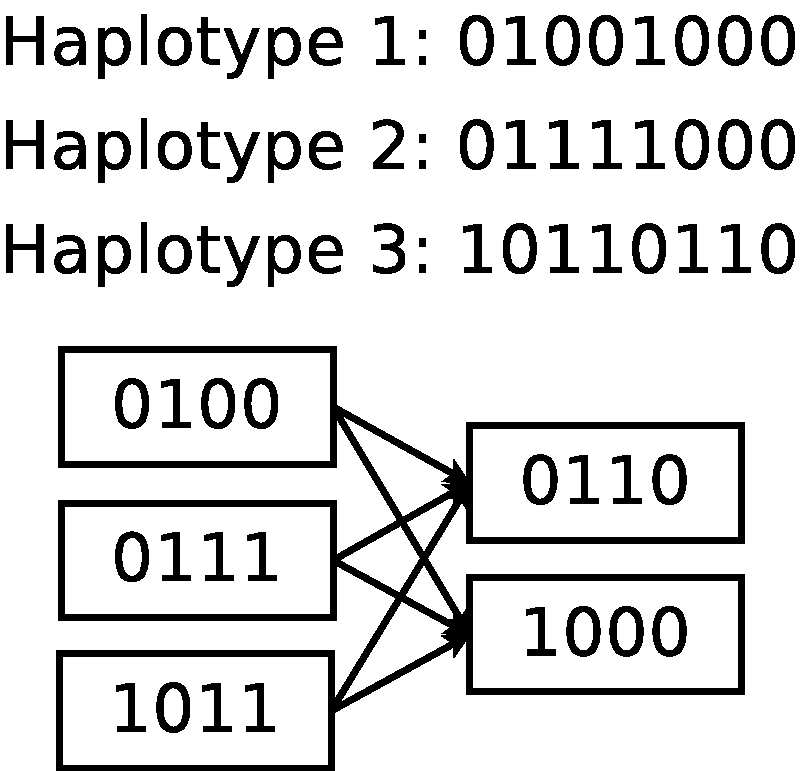
\includegraphics[width=.45\textwidth]{chap3figs/hapiur}
  \caption[The HAPI-UR haplotype model]{The HAPI-UR haplotype graph.  The three conditioning haplotypes are represented in the graph structure pictured below them. All haplotypes are distinct for the first four markers, creating three distinct states.  The last four markers are the same for the first two haplotypes allowing them merge to the same state.  This representation reduces both the state space and the number of locations where transitions can occur. In practice, the length of the segments is allowed to vary.\label{chap3:hapiur}}
\end{SCfigure}

 Figure~\ref{chap3:hapiur} gives a toy example of this graph across eight markers with three observed haplotypes. The markers are split into two segments with three and two states respectively.  This graph not only reduces the statespace but also the number of locations where state transitions can occur.  This graph structure is similar to one used in SHAPEIT1 but with the key difference that the number of markers per segment is allowed to vary within the model. The edges are weighted via modified Li and Stephens model and no mutation events are allowed, so an individual's haplotypes have to exactly match a path through this graph.  This rather rigid model allows very fast inference but comes at some cost in flexibility, new states need to be added to the graph for a single base pair change.  HAPI-UR is currently the fastest algorithm for unrelated individuals, but is less accurate than SHAPEIT2.  The recommended pipeline for HAPI-UR is to run it three times with different seeds, then the outputs from individual runs ``vote'' on the phase at each heterozygous locus. We follow this procedure in our experiments and denote the method as ``HAPI-UR 3X''.
\clearpage
\section{Phasing explicitly related individuals}
The phasing methods described in the previous section infer haplotypes by leveraging linkage disequilibrium, which typically reflects very distant relatedness of an unknown degree between individuals within a sample.  When we deal with explicit pedigrees containing very close relationships, the model we need to use is simpler (at least conceptually). We know a child receives one haplotype from each parent and that we can expect very few recombination crossover events per chromosome, meaning the haplotype a parent \emph{transmits} to a child is a mosaic of that parent's two haplotypes containing very few breaks.  Routines for using parent-child (duo) and mother-father-child (trio) relationships are included in SHAPEIT2, Beagle and HAPI-UR and we describe how these work here.  Routines for complex pedigrees of general structure require more specialised inference machinery, probably the most well known being the Lander-Green algorithm of which we also give an overview.  We also discuss the limitations of each of these approaches.

\subsection{Simple Duo/Trio Phasing}
Given a father-mother-child trio and ignoring crossover events (of which there are only several per chromosome) we only need to consider four haplotypes for the six individuals.  These are the two haplotypes the child receives from its parents (transmitted) and their complements (untransmitted).  Enforcing Mendelian inheritance then constrains the phase at any site that is not heterozygous throughout the pedigree. In the case of SHAPEIT2 this is achieved by placing constraints on its segmented haplotype graph. Beagle performs this by modelling the trio as four independent haplotypes and sampling haplotypes (based on its graph) that are consistent with the trio data~\citep{browning2009unified}. This simple Mendel phasing is relatively easily to integrate with LD based phasing methods, and will result in the same haplotype estimates as the more sophisticated Lander-Green algorithm (described next) in the case of a standalone duo or trio.  

Whilst useful, the duo/trio phasing available in several standard software packages has limitations. It does not elegantly generalise to larger complex pedigrees, such pedigrees could partitioned into small duos and trios but this is sub-optimal.  Consider a nuclear family with five children, it could be partitioned into two duos, but one child would not be able to exploit any parental relationship.  It is uninformative of meiosis, Figure~\ref{chap3:trio} shows a trio with its true underlying haplotypes (left) and those inferred by Mendel phasing (centre), a switch error is induced on the paternal haplotypes due to a crossover event. Crossovers are of course rare so this is not a serious issue unless a researcher wishes to study recombination.  Mendel phasing is also sensitive to genotyping error.  Genotyping errors that cause Mendelian inconsistent genotypes will be flagged as missing in any sensible QC pipeline, for example a site where the mother was AA, the father was AA and the child was BB would be flagged as missing throughout the pedigree.  However not all errors cause Mendelian inconsistency, and if these are left in the data they can induce a switch error throughout the pedigree, see figure~\ref{chap3:trio} right.  

\begin{figure}[h]
\vspace{20pt}
  \begin{center} 
    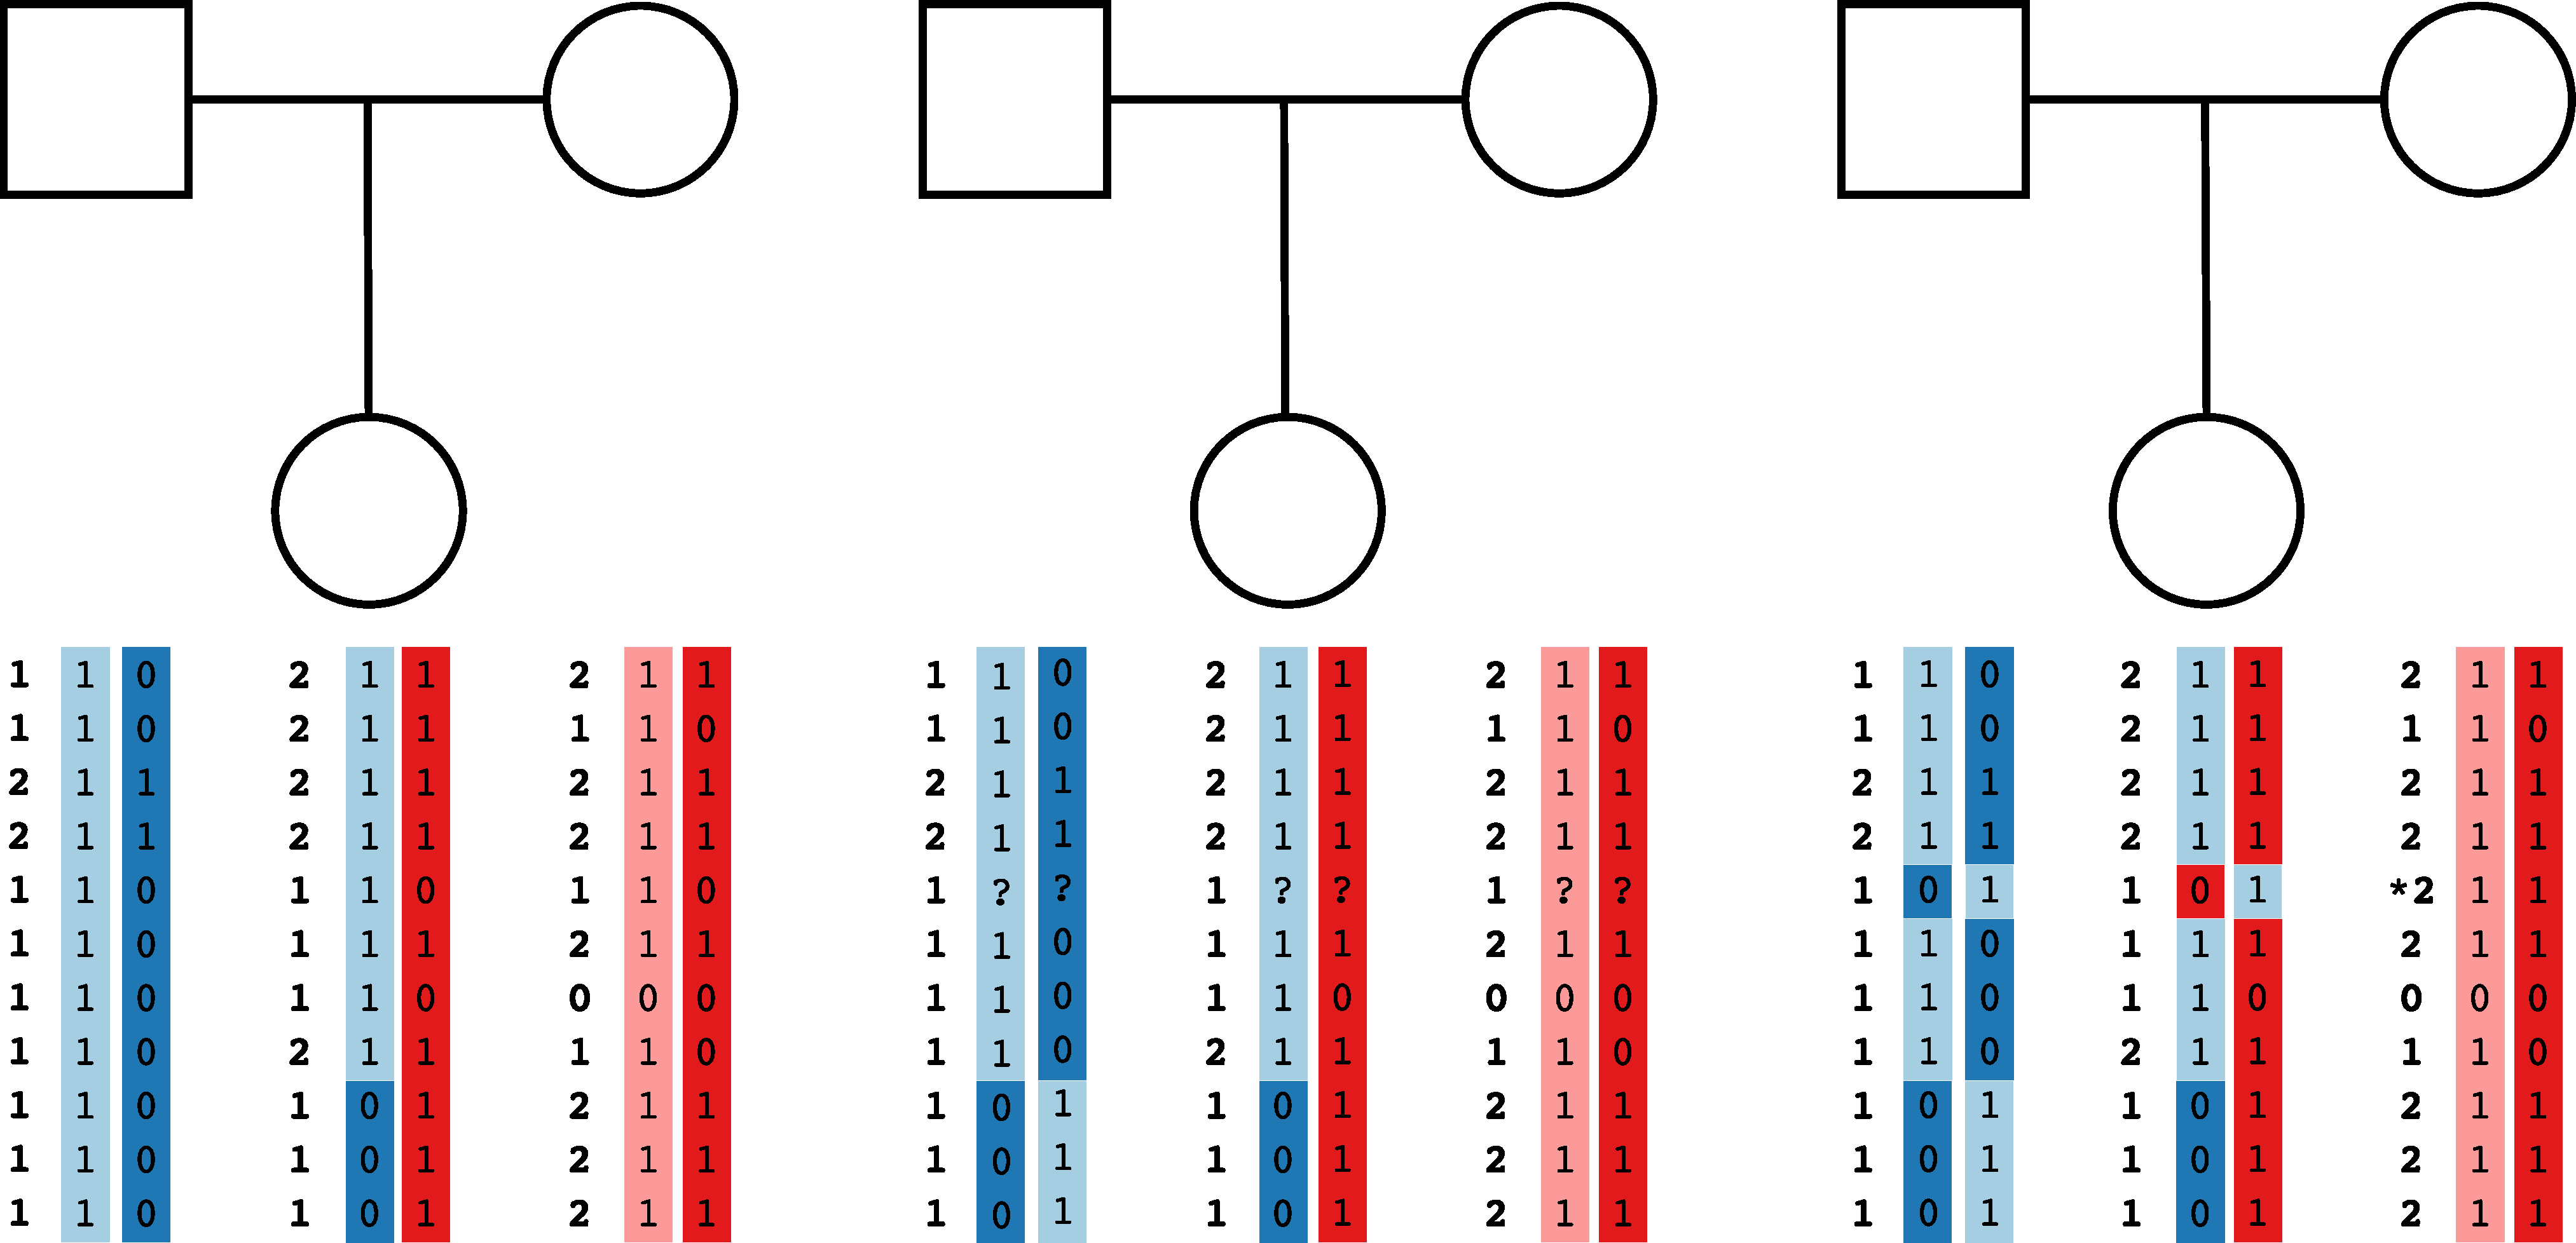
\includegraphics[width=\textwidth]{chap3figs/trio}
    \caption[Father-mother-child trio phasing examples]{Father-mother-child trio phasing examples.  The paternal haplotypes are in light/dark blue and the maternal in light/dark red.  Genotype values are to the left of haplotypes.  \textbf{Left:} True underlying haplotypes, a crossover event has occurred on the paternal meiosis meaning the child's haplotype is a mosaic of the father's two haplotypes. \textbf{Centre:} The haplotypes that will be inferred by phasing with Mendel's rules.  The site that is heterozygous in all three individuals cannot be phased with the pedigree information alone, but will be resolved using LD information from the wider population. The father's haplotypes have been inferred as the transmitted and untransmitted haplotypes (the recombined haplotypes) inducing a switch error.  Since there are very few crossovers per chromosome this is not a serious issue unless we wish to study recombination explicitly.  \textbf{Right:}  A genotyping error has been introduced in the mother (denoted by *) this causes incorrect phasing to propagate to the father and child.  Since the error is still Mendelian consistent, it is difficult to detect.\label{chap3:trio}}
  \end{center} 
\end{figure}
\clearpage
\subsection{The Lander-Green Algorithm}

The simple Mendel phasing rules described in the previous section do not elegantly generalise to situations where there is $>1$ meiosis present in a pedigree since parents transmit different haplotypes to different siblings due to recombination.  The Lander-Green (LG) algorithm~\citep{lander1987} finds the most likely haplotypes for individuals in a pedigree, conditional on the pedigree structure and the individual's genotypes.  The algorithm is computationally expensive, and there have been many clever implementations (and approximations) to improve efficiency~\citep{sobel1996descent,gudbjartsson2000allegro,abecasis2002merlin,lange2013mendel}. We describe a na\"{\i}ve implementation here. 

Given a pedigree with $N_F$ founders and $N_D$ descendants (and hence $N_D$ meioses), there are $2^{2N_D}$ possible patterns of gene flow (which founder haplotype a descendant has inherited) in the pedigree.  Patterns of gene flow can change due to recombination events as we move along the chromosome. Figure~\ref{chap3:landergreen} visualises the gene flow for a three sibling nuclear family with paternal (P), maternal (M) and child (C1-C3) haplotypes. There are two changes in gene flow due to recombinations in first the paternal meiosis (to C2) and then the maternal meiosis (to C3). This process can be modelled as a Markov chain with $2^{2N_D}$ possible states across the chromosome with transition probabilities calculated from the genetic distance between markers and with emission distribution that is a function of allelic frequencies.  

We enumerate each possible inheritance pattern at site $l$ and store them in inheritance vector $V_l$ of length $2N_D$. The $(2i-1)$th position of this vector is 0 if the $i$th non-founder individual received their parents first haplotype and 1 if they received the second.  The $(2i)$th position has the same property but for the maternal chromosome.  The pattern of inheritance can change across the chromosome so we have a sequence of inheritance vectors, $V=\{V_1,\ldots,V_L\}$ .  These vectors are visualised (along with changes due to crossovers) in the bottom row of figure~\ref{chap3:landergreen}.

\begin{figure}
  \begin{center} 
    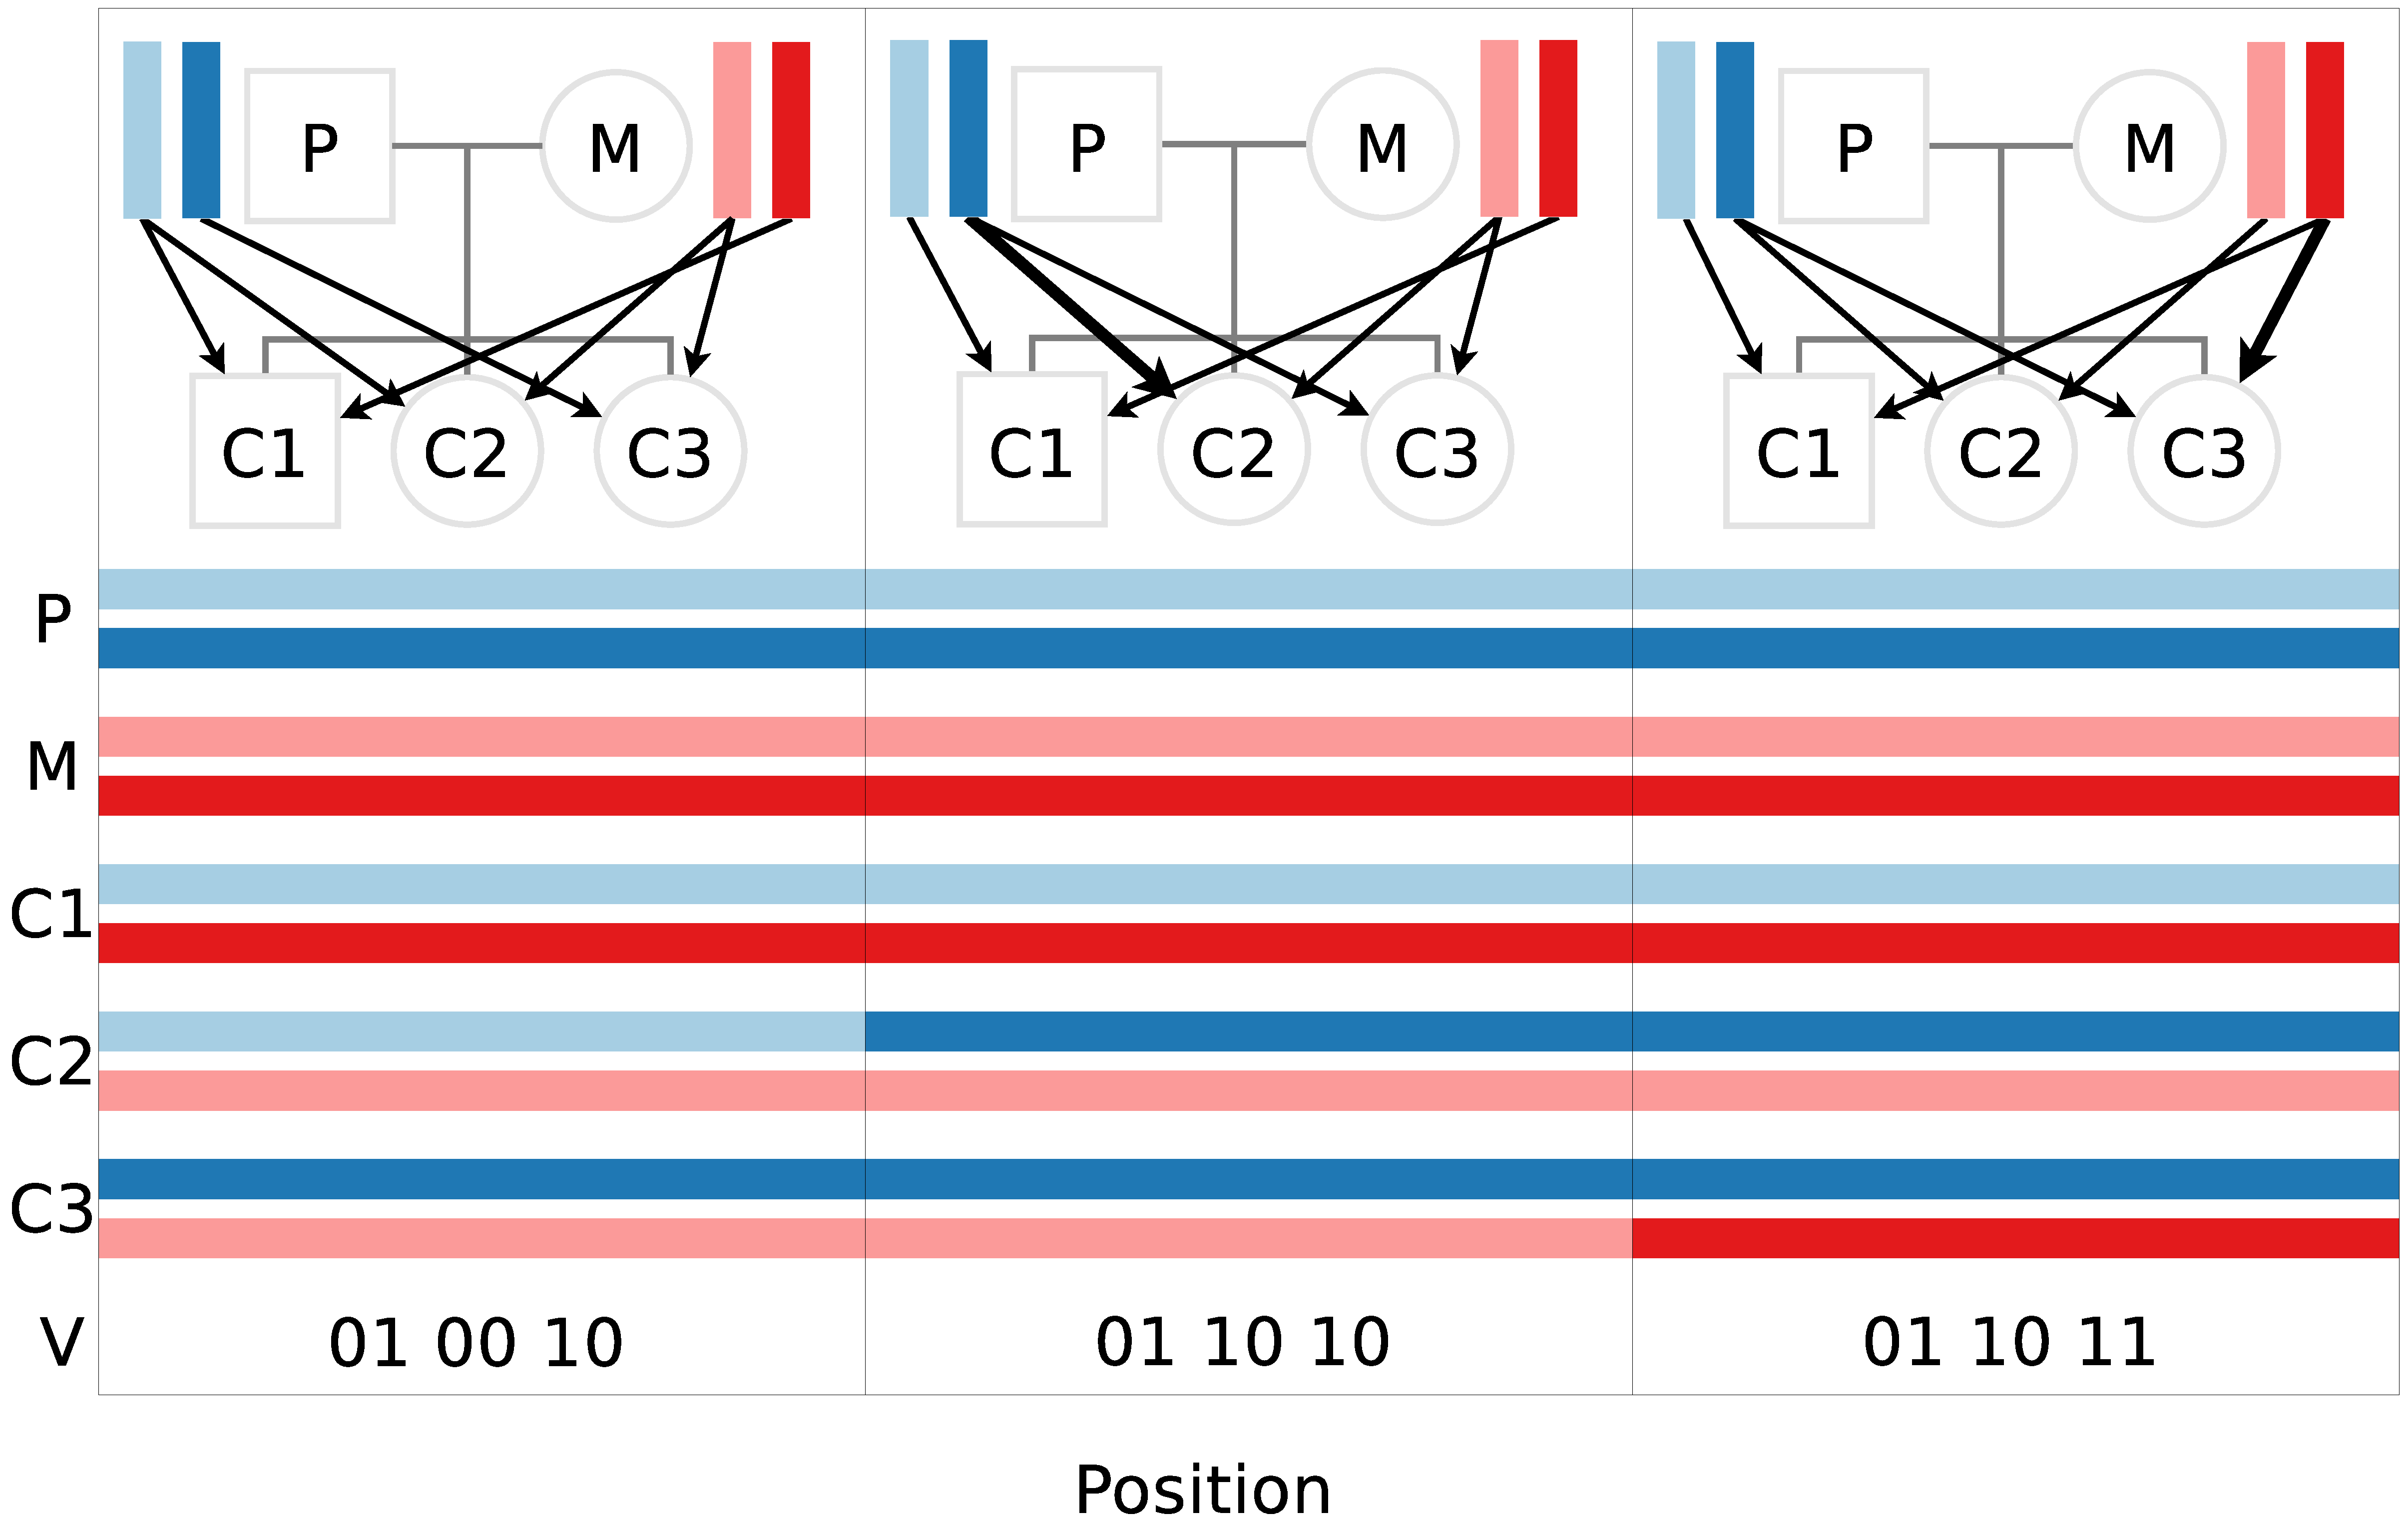
\includegraphics[width=\textwidth]{chap3figs/nuclear_family}
    \caption[The Lander-Green haplotype model]{An example of the Lander-Green Markov process for a three sibling nuclear family.  The paternal (P) chromosomes are in blue and the maternal (M) in red.  Children C1, C2 and C3 receive one (possibly recombined) chromosome from each parent coloured accordingly. The horizontal bars denote the haplotypes of individuals across a genomic region, with the colour of the bar changing when a crossover has occurred on the haplotype received from the parent. The edges in the pedigree diagram indicate the current state of gene flow, with the bold edge indicating a change in inheritance from the previous position. The state $V$ is the binary inheritance vector representing the gene flow pattern at each position.  \label{chap3:landergreen}}
  \end{center} 
\end{figure}
  
\clearpage
The inheritance pattern can change between sites $l$ and $l+1$ according to the transition  matrix $\T_l^{\otimes 2N_D}$, which is calculated by recursively taking the Kronecker product of the matrix
\[ \T_l  = \left[
  \begin{array}{c c}
1 - \rho_l &   \rho_l \\
 \rho_l & 1 - \rho_l  \\
  \end{array}  
\right] \]
with
\[ \T_l^{\otimes n + 1}  = \left[
  \begin{array}{c c}
    (1 - \rho_l)\T^{\otimes n} &  \rho_l\T^{\otimes n} \\
    \rho_l\T^{\otimes n} & (1 - \rho_l)\T^{\otimes n}  \\
  \end{array}  
\right] \]

where $\rho_l$ is the per-generation recombination rate between sites $l$ and $l+1$. The matrix $\T_l^{\otimes 2N_D}$ is then a symmetric $2^{2N_D} \times 2^{2N_D}$ matrix where the diagonal corresponds to 0 crossovers for all meioses.  The transition probability $P(V_{l+1}=k|V_l=k')$ is then the $(k,k')$th entry of $\T_l^{\otimes 2N_D}$.  

We also require the emission distribution which is 
$$ P(G_l|V_l)  = \sum_a \prod_{i=1}^{2N_F} f_{a_i}$$
where $a=[a^1,\ldots,2^{N_F}]$ enumerates every possible set of founder (haploid) alleles that are consistent with $G_l$ and $V_l$, and $f_{a_i}$ is the frequency of allele $a_i$.  

The likelihood for this process is then:
$$L(G) = \sum_V P(V_1) \prod_{l=1}^{L-1} P(V_l|V_{l+1}) \prod_{l=1}^L P(G_l|V_l) $$
 
We can apply the Viterbi algorithm to this likelihood to obtain the most likely sequence of inheritance vectors across a chromosome and then choose the most likely set of alleles from  $a$, for $V_l$. Note that for bi-allelic loci, when at least one individual at site $l$ is homozygous then there is at most one possible $a$ per state. When all individuals are heterozygous there are two equally likely versions of $a$ meaning phase cannot be reliably assigned.

The Mendel phasing rules for duos/trios described at the start of this section are actually a special case of phasing with the LG algorithm.  When there is only one descendant present in a pedigree the emission distributions for each possible gene flow pattern will be equal and since the probability of recombination between markers are typically $\rho_l << 0.5$ there will be no state transitions.  This means that there are four equally likely state paths across the chromosome where the state is just one of the four possible inheritance patterns and is unchanging across the chromosome.  Each path corresponds to a different arbitrary ordering of parental haplotypes.  This is an example of what we will refer to as an \emph{uninformative} meiosis, in that it is uninformative towards recombination events. We define \emph{informative} meioses as those where either grandparents are genotyped or $>2$ siblings are genotyped. Such data allow us to determine crossover events unambiguously.

\subsubsection{Limitations of the LG approach}

\paragraph{Complexity}
A na\"{\i}ve implementation of the LG algorithm must evaluate $2^{2N_D} \times 2^{2N_D}$ possible state transitions between loci giving the algorithm exponential complexity $O(2^{4N_D}L)$. Merlin utilises sparse binary trees to avoid unnecessary calculations such as inheritance patterns that are either impossible (incompatible with observed genotypes) or are equally likely (redundant) making it more efficient than a na\"{\i}ve implementation.  However computation still scales exponentially and pedigrees with say $N_D>30$ non-founders are intractable to analyse.  In practice such large pedigrees can be partitioned for tractable analysis so this issue is largely one of inconvenience.

\paragraph{Sensitivity to genotyping error}
Non-Mendelian genotyping errors that induce switch errors such as that pictured in figure~\ref{chap3:trio} (right) can often only be accommodated via unlikely patterns of recombination with the erroneous marker typically being flanked by two crossover events.   Merlin and other pedigree software provide some functionality to detect probable errors based on these unlikely recombination patterns.  Genotypes at these loci can then be marked as missing throughout a pedigree. However the power to detect errors decreases with pedigree size and is non-existent for parent-child duos and father-mother-child trios.

\paragraph{Resolution of heterozygous sites throughout a pedigree}
Heterozygous founder genotypes where neither haplotype passes through a homozygote descendant cannot be resolved (both haplotypes are equally likely under the LG model).  For research groups applying pre-phasing and imputation pipelines, which are now a standard part of GWAS, this is particularly problematic.  Such incomplete haplotypes cannot be readily used with available imputation software.  Whilst it would be possible to incorporate these haplotype constraints into, say the SHAPEIT2 segmented graph, such functionality would be complicated to implement.

\section{Long-Range Phasing}
 As sample sizes increase, becoming a substantial fraction of the total population (>1\%), the chances of an individual having a recent ancestor in the sample becomes substantial. At any particular location, the chance of two individuals inheriting genetic material from an ancestor $M$ generations ago rapidly becomes small with probability equal to $2^{-2M+1}$, but when common material is inherited it will be a relatively large tract of DNA that is distributed approximately exponentially with mean $100M^{-1}$ centiMorgans~\citep{browning2012identity}.  This sharing of relatively large haplotypes has been referred to as `long-range LD'  \citep{kong2008detection}.

This long range sharing of haplotypes can be exploited to aid haplotype estimation. This idea was first proposed by  \cite{kong2008detection} who made the observation that sampling a large enough fraction of a population (which was possible in the rather unique Icelandic population) will increase the chance that two individuals will share a long region of genetic material IBD. A method was proposed in which `surrogate parents' (IBD sharers) are identified for each individual in a given region of the genome. These surrogate parents allow the haplotypes to be determined with high accuracy using Mendel's rules, effectively as if the true parents had been observed and the family could be phased as a trio.  Kong described a rule based approach and applied it to a large cohort of individuals from Iceland  to produce highly accurate haplotypes. Whilst this was a novel idea, software for general use was not provided.

\subsection{The Systematic Long Range Phasing Algorithm}
Systematic Long Range Phasing (SLRP)\citep{palin2011identity} implements a probabilistic approach to this problem and jointly models the IBD status of all individuals.  The IBD status for each pair of individuals $i$ and $j$ is modelled as a Markov process with hidden state $V^{i,j}_l \in \{1,2,3,4,5\}$ for $l=1\ldots L$ where the states correspond to; 
\begin{enumerate}
\item No IBD
\item IBD between the first two haplotypes
\item IBD between the first haplotype of $i$ and second of $j$
\item IBD between the second haplotype of $i$ and first of $j$ 
\item IBD between the second two haplotypes
\end{enumerate}
We can write the joint distribution of $H$ and $V$ given genotype data $G$ as
\begin{eqnarray*}
  P(H,V|G) &  \propto & P(G|H,V)P(H,V) = P(G|H)P(V|H)P(H) \\
  & = & \prod_{i=1}^N \prod_{l=1}^L \Bigg( P(G_{il}|H_{(2i-1)l},H_{(2i)l}) P(H_{(2i-1)l},H_{(2i)l})\\
&&~~~~~~~~~~~~\times \prod_{j=i+1}^N P(V_l^{i,j}|V_{l-1}^{i,j},H_{(2i-1)l},H_{(2i)l},H_{(2j-1)l},H_{(2j)l})\Bigg)\\
\end{eqnarray*}
The first two terms here are straightforward. SLRP does not model genotyping error so $P(G_{il}|H_{(2i-1)l},H_{(2i)l})$ is just an indicator variable on whether the haplotypes are consistent with the genotype. A flat prior is used for $P(H_{(2i-1)l},H_{(2i)l})$.  

The final term can be factorised to obtain
$$P(V_l^{i,j}|V_{l-1}^{i,j},H_{(2i-1)l},H_{(2i)l},H_{(2j-1)l},H_{(2j)l})\propto P(V_l|V_{l-1}) P(H_{(2i-1)l},H_{(2i)l},H_{(2j-1)l},H_{(2j)l}|V^{i,j}_l)$$
the emission distribution on the haplotypes is simply the product of the four allele frequencies if not in IBD or the product of
 three allele frequencies if the individuals are in IBD. 

The IBD transition probabilities, $P(V_l|V_{l-1})$, come from a continuous time Markov process with rate parameters $\lambda_\textrm{NOIBD}$ for $V=1$ and $\lambda_\textrm{IBD}$ for $V\neq1$ with the constraints that IBD states always transition to the non-IBD state and the non-IBD state transitions to the four IBD states with equal probability.  Hence the transition probabilities between markers $l$ and $l+1$ are 
\[ P(V_{l+1}=k|V_l=k') = \left\{
\begin{array}{c c} 
  e^{\lambda_\textrm{NOIBD} \rho_l}) & k'=1,k = 1 \\
  \frac{1}{4}(1-e^{\lambda_\textrm{NOIBD} \rho_l}) & k'=1,k \neq 1 \\
   e^{\lambda_\textrm{IBD} \rho_l} & k'\neq1,k\neq1,k=k' \\
  1- e^{\lambda_\textrm{IBD}\rho_l} & k'\neq1,k= 1 \\
  0   &  \textrm{otherwise} \\
\end{array}  
\right.\]
SLRP fits this model as a Bayesian network and produces MAP estimates of the both $H$ and $V$.  
%% \[ P(Z_{l+1}=k|Z_l=k')  = \left\{ 
%%   \begin{array}{l l}
%%     \exp(-\frac{\rho_l}{K}) + \frac{1-\exp(\frac{\rho_l}{K})}{K} & \quad k = k'\\
%%     \frac{1-\exp(\frac{\rho_l}{K})}{K} & \quad k \neq k'
%%   \end{array}  \label{chap3:listephentrans}
%%   \right.\]


\subsection{Limitations of Long-Range Phasing}Both the original approach by \cite{kong2008detection} and SLRP  demonstrated very accurate haplotype estimates within IBD regions, but suffer from the problem that phase can only be inferred for genomic regions where IBD sharing is found.  Even in IBD regions, if all individuals are heterozygotes, the phase at that particular locus cannot be inferred.  This is essentially the same problem encountered in pedigree phasing, only partial haplotypes are inferred.  These partial haplotypes could potentially be `filled in' by one of the LD approaches described above, in a manner similar to duo/trio phasing.  Computational complexity is also an issue, SLRP evaluates $N(N-1)/2$ HMMs (every pair of individuals) meaning computational complexity is $O(N^2L)$. This limits the sample sizes that can be tractably analysed.

\section{Integrating extended pedigree information into SHAPEIT2 haplotypes}
\label{chap3:duohmm}
The Lander-Green algorithm is traditionally the method of choice for phasing pedigrees but has several limitations described previously.  The results in the next chapter demonstrate that SHAPEIT2 can in fact phase extended pedigrees extremely accurately, even when completely ignoring any pedigree relationships.  Given this result, there seemed little need to implement a sophisticated LG algorithm within the SHAPEIT2 software itself.  However we would still like to take advantage of the pedigree information for maximum accuracy. 

 We developed a method for analysing SHAPEIT2 haplotypes in a post-hoc fashion when pedigrees are present within a cohort.  First SHAPEIT2 is run ignoring all familial relationships, that is,
 all individuals are treated as if they were unrelated. We then apply a simple HMM to the SHAPEIT2 haplotypes that corrects phasing errors that are inconsistent with pedigree information and to detect subtle genotyping errors. The method focuses on each parent-child duo separately and this circumvents several issues with the Lander-Green algorithm, namely;
\begin{itemize}
\item \emph{complexity}: our HMM has 4 states so there are 16 possible state transitions for each meiotic event, so our method scales as $O(N_DL)$ where $N_D$ is the number of non-founders and $L$ is the number of markers. This compares well to the $O(2^{4N_D}L)$ scaling for a na\"{\i}ve Lander-Green implementation.
\item \emph{heterozygous markers}: markers that are heterozygous throughout a pedigree will be phased via leveraging population haplotypes
\item \emph{sensitivity to genotyping error}: the low computational complexity of the model allows us to accommodate genotype uncertainty
\end{itemize}
We describe the model and several useful applications of it below, we refer to this framework as the duoHMM in later sections of the thesis.
\subsection{The Duo HMM}
Let $p = (p_1, p_2)$ and $c = (c_1, c_2)$ denote a pair of observed (ordered) parental and child haplotypes respectively. Here $p_i = \{p_{i1},\ldots, p_{iL}\}$ denotes the $i$th parental haplotype at the $L$ sites across a chromosome. The same notation is used for the $i$th child haplotype $c_i$. There are four possible patterns of gene flow between the parent and child. The true pattern of gene flow will remain constant over long stretches of a chromosome due to the low rate of recombination in any given meiosis. We use $S_l$ to denote the pattern of gene flow at the $l$th locus, where $S_l = (j,k)$ means that the parents $j$th haplotype and the child's $k$th haplotype are identical by transmission (IBT). Here $j,k \in \{1,2\}$, so there are just four possible transmission patterns, which we denote $A=(1,1), B=(2,1), C=(1,2), D=(2,2)$. The true transmission states $S=\{S_1, \ldots,S_L\}$ are unobserved across each chromosome and we wish to infer them from our imperfect observations of the parental and child haplotypes $p$ and $c$. The intuition behind our approach is that true recombination events and switch errors will cause changes to the pattern of gene flow as we move along a chromosome. Thus we can think of the observed pattern of gene flow as the superposition of two point processes: one with a rate dictated by true recombinations, and a second process with a rate relating to switch errors. Our aim is to deconvolve these two processes to detect the true recombination events and correct switch errors. 

To carry out this inference we have developed an HMM that allows for switch errors in the parental and child haplotypes. We use $\delta_1$ and $\delta_2$ to denote the probability of a switch error on the parental or child haplotypes between two adjacent markers respectively. We also use  $\rho_l$ to denote the probability of a recombination occurring between markers $l$ and $l+1$. Specifically we use $\rho_l = 1 - e^{-r_l}$ where  $r_l$ is the genetic distance between markers $l$ and $l+1$.  We use the genetic distances from the HapMap LD based map \citep{InternationalHapMapConsortium:2005cu} (which are inherently sex averaged) and scale them to the sex-specific genetic lengths from the deCODE 2002 map \citep{kong2002} according to the sex of the parent.

The initial states of the Markov model are given by $P(S_1) = 1/4$. The transition rates on the IBT states $S$ are then given by 
\small
\[ P(S_{l+1}=v|S_l=u) = \left\{ \begin{array}{ll}
    (1-\delta_2) \times \left((1-\delta_1)(1-\rho_l) + \delta_1\rho_l \right)& \mbox{if } (u,v) \in T_1\\
    (1-\delta_2) \times \left((1-\delta_1)\rho_l + \delta_1(1-\rho_l) \right) & \mbox{if } (u,v) \in T_2\\
    \delta_2 \times \left( (1-\delta_1)(1-\rho_l) + \delta_1\rho_l \right) &  \mbox{if } (u,v) \in T_3 \\
    \delta_2 \times \left( (1-\delta_1)\rho_l + \delta_1(1-\rho_l) \right)&  \mbox{if } (u,v) \in T_4   
\end{array} \right. \] 
\normalsize
The sets $T_1, T_2, T_3, T_4$ denote the different types of transition that can occur. The set $T_1 = \{(A,A), (B,B), (C,C), (D,D)\}$ contains the transitions where no change in gene flow occurs. The set $T_2 = \{(A,B), (B,A), (C,D), (D,C)\}$ are the transitions with a change only to  which of the parent's haplotypes are IBT. The set $T_3 = \{(A,C),(B,D),(C,A),(D,B)\}$ are the transitions with change only to which of the child's haplotypes are IBT. The set $T_4 = \{(A,D),(B,C),(C,B),(D,A)\}$ are the transitions with a change to both of child and parental IBT haplotypes. Figure~\ref{fig:duo_hmm_examples} shows examples of how true recombination events and switch errors in parental or child haplotypes lead to changes in the transmission pattern in terms of $T_2$, $T_3$ and $T_4$ events.

We accommodate genotyping error by allowing for errors in the emission part of the HMM. We model the observed haplotypes at the $l$th locus conditional upon the transmission state $S_l$ as follows
\[ P(p_l, c_l | S_l=(j,k)) = \left\{ \begin{array}{ll}
1-\epsilon & \mbox{if } p_{lj}=c_{lk}\\
\epsilon & \mbox{if } p_{lj}\neq c_{lk}\\
\end{array} \right. \] 
Our full model can then be written down as 
\[P(p, c, S) = P(S_1)\prod_{l=1}^{L-1} P(S_{l+1}|S_l) \prod_{l=1}^L P(p_l, c_l | S_l).\]

This method can be applied to any set of estimated haplotypes from parent-child pairs. We run one iteration of the Forward-Backward algorithm, to estimate $\epsilon$, $\delta_1$ and $\delta_2$.   Since there is little uncertainty in the state path this was found to be adequate for convergence. This estimation is carried out on each duo separately. Since the HMM has just four states the computation involved is negligible.

\begin{figure}[p]
 \begin{center} 
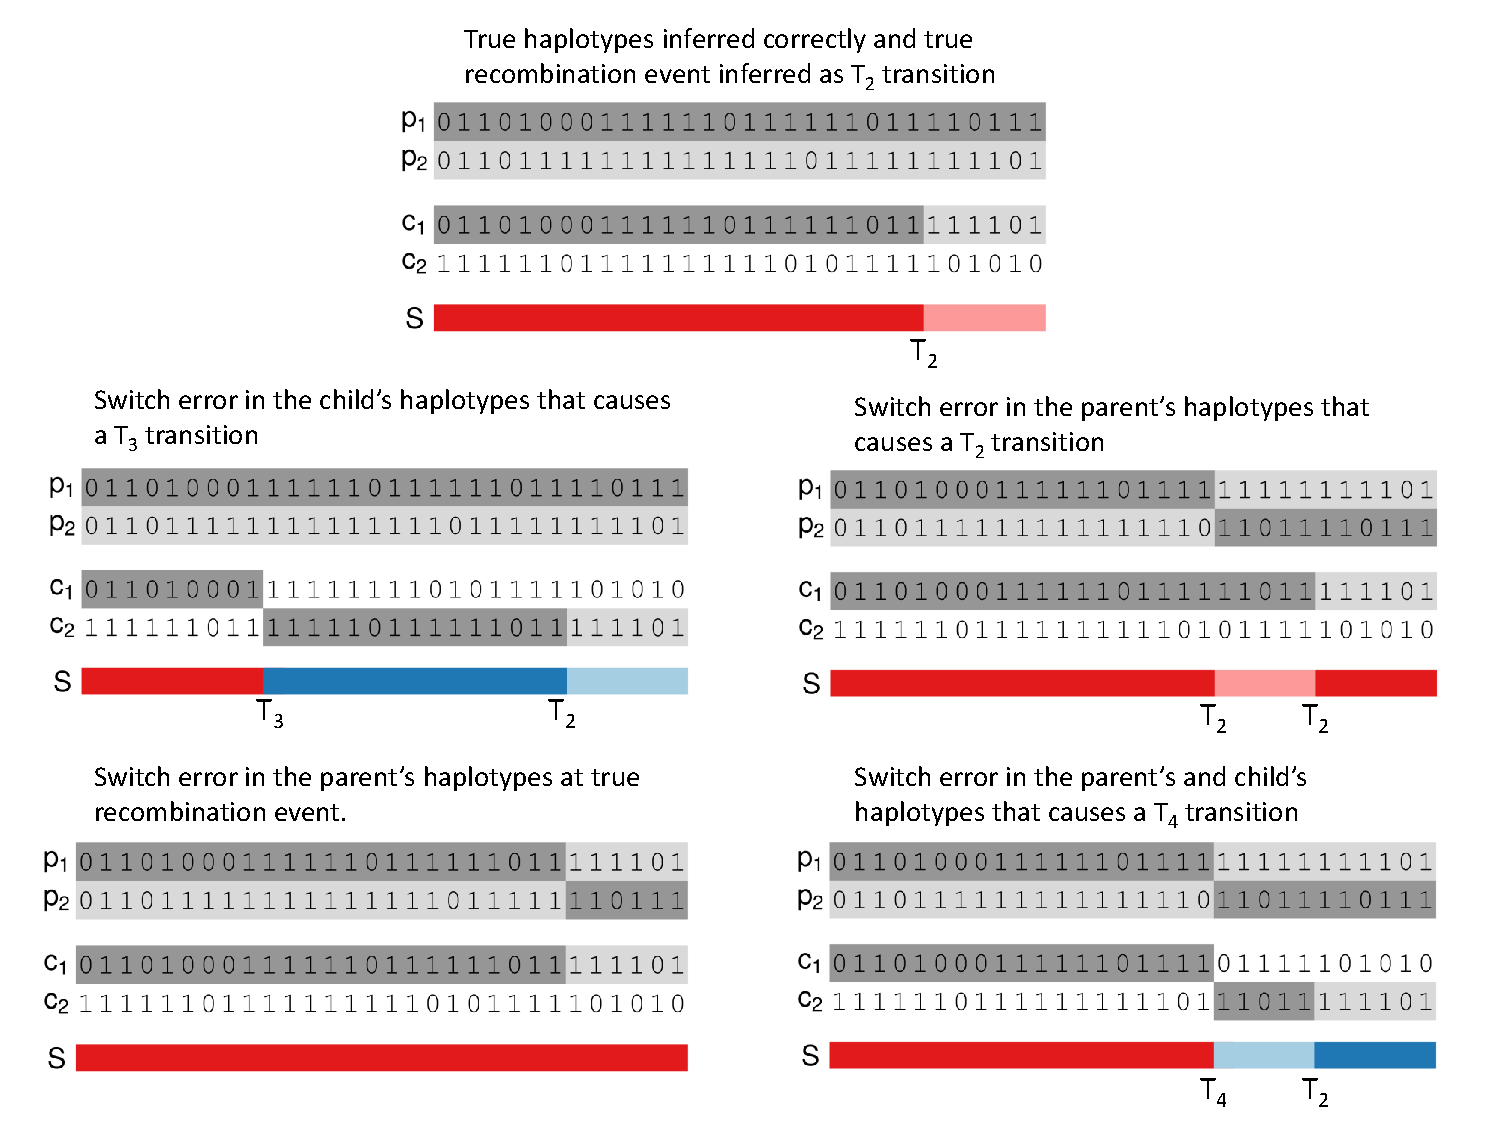
\includegraphics[width=\textwidth]{chap4figs/Fig2}
   \caption[Examples of DuoHMM model]{Examples of inferred haplotypes with true recombination events and switch errors. In each examples $p_1$, $p_2$, $c_1$ and $c_2$ denotes the two parental and child haplotypes and $S$ denotes the pattern of gene flow. \textbf{Top:} Correctly inferred haplotypes in a region of a true  recombination event that causes a $T_2$ transition in the duo HMM. The other 4 examples in the figure add switch errors to these true parental and child haplotypes. \textbf{Middle~left:} addition of a switch error in the child's haplotypes that causes a $T_3$ transition. \textbf{Middle~right:}  addition of a switch error in the parent's haplotypes that causes a $T_2$ transition. \textbf{Bottom~left:} addition of a switch error in the parent's haplotypes at the site of the recombination event that causes the $T_2$ transition to be missed. \textbf{Bottom~right:} addition of a switch error in both the child's and parent's haplotypes at the same position that causes a $T_4$ transition.\label{fig:duo_hmm_examples}}
 \end{center} 
\end{figure}

\subsection{Correcting haplotypes}

We now describe how to use our model to adjust haplotypes so that they are consistent with a given pedigree structure. After estimating parameters, we run the Viterbi algorithm to find the most likely state sequence.  There are sixteen possible state transitions in our model. The eight transitions in the sets $T_3$ and $T_4$ imply a switch error in the child haplotypes, so when we observe one of these transitions in the Viterbi sequence we infer a switch error in the child. The eight transitions in the sets $T_2$ and $T_4$ imply either a switch error or a recombination event in the parental haplotypes. Inferring whether a recombination or a switch error has occurred in the parental haplotypes is difficult. When more than one sibling is present in a pedigree, we can correct probable parental switch errors via identifying the minimum recombinant haplotypes for the family.  When one of the $T_2$ or $T_4$ transitions is present in the same location for the majority of siblings, this is most likely a switch error on the parental haplotypes and they can be corrected accordingly (see  Figure~\ref{fig:correction_example}) for an example of this process). This is not strictly the maximum-likelihood solution, but the minimum-recombinant and maximum likelihood solutions often yield the same result \citep{williams2010rapid}. When we infer a switch error in either a parent or a child we correct the haplotypes by switching the haplotype phase of all loci proceeding the switch error. This procedure is carried out left to right along the sequence. 


\begin{figure}[h]
  \begin{center} 
   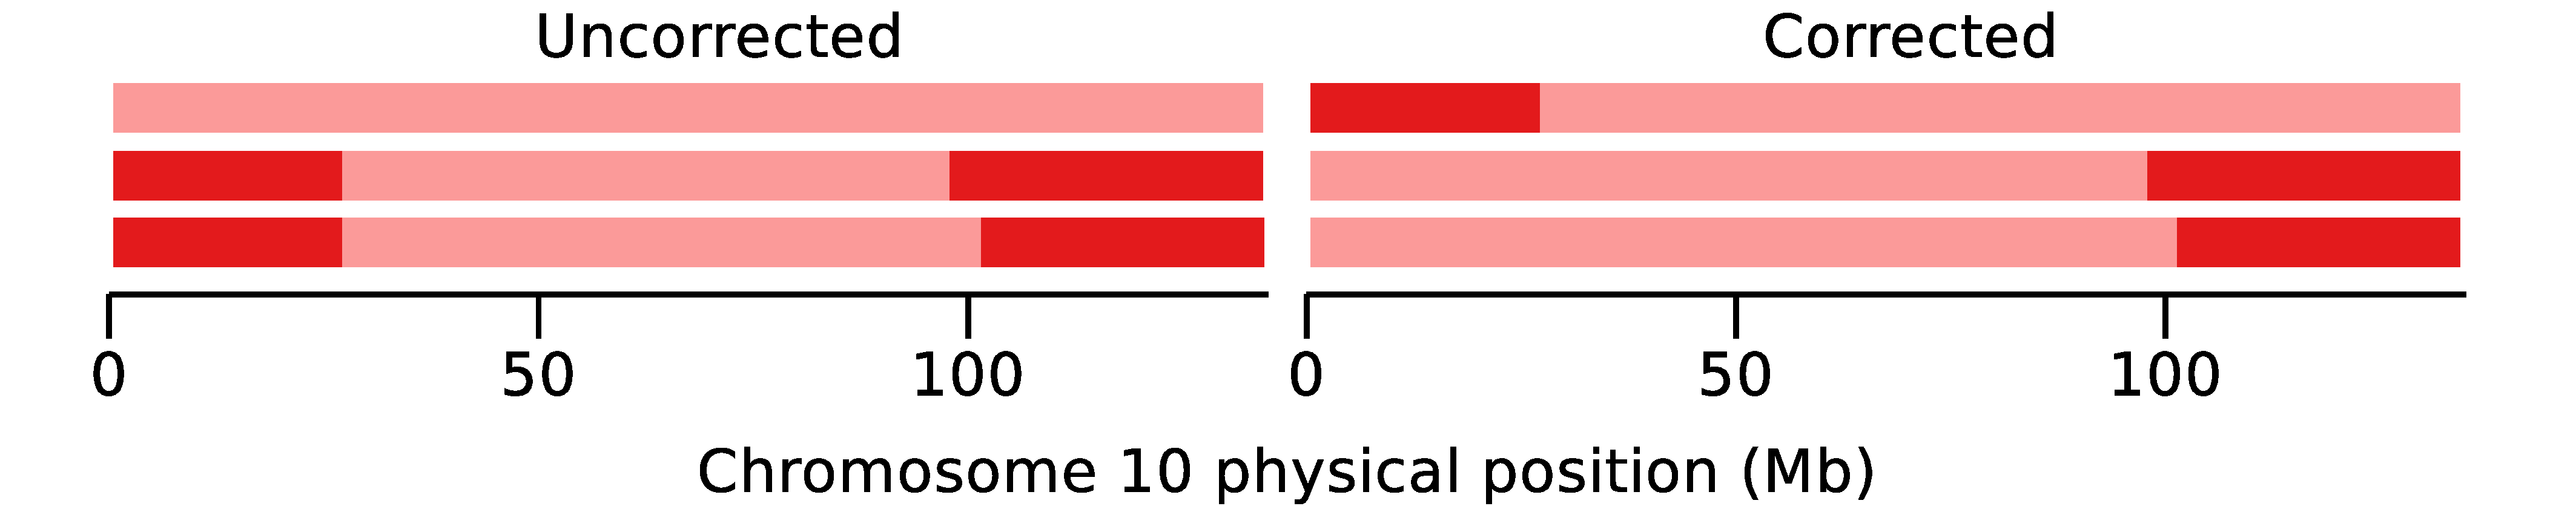
\includegraphics[width=\textwidth]{chap3figs/correction_example}%\vspace{-20pt}    
  \end{center} 
\caption[Haplotype correction example using the DuoHMM]{Haplotype correction example using the DuoHMM. The Duo HMM Viterbi paths for a three father-child duos from a nuclear family (ie. 3 siblings) from the FVG cohort on chromosome 10. The four possible IBT states (A, B, C, D) are shown using colours pale blue, dark blue, light red and dark red respectively (although states A and B do not occur in this example).  The left panel shows the path prior to any corrections, and the right panel after a minimum recombinant correction is applied.  The second and third sibling initially had a $C \rightarrow D$ transition at around 25mb, this is more likely a recombination event in the first child hence the parental haplotypes are switched after this point.  The panel on the right has the corrected haplotypes, the number of recombination events required to explain the observed data has been reduced.\label{fig:correction_example}}
\end{figure}

Corrections are applied sequentially `down' through each pedigree. For example, in a three generation (grandparent-parent-child) pedigree we first apply the method to those duos containing grandparents. Any corrections made to the parents haplotypes are used when processing duos involving those parents and their children. This removes any (detectable) switch errors for individuals that have parents, before their descendants are phased. 

\subsection{Detecting recombination events}
Once all the haplotypes have been corrected the duo HMM is re-run in order to infer recombination events. We do this by calculating the probability of a recombination event between markers. A transition between the parental haplotypes corresponds to either a switch error or a genuine recombination.  A recombination event can only be resolved down to the region between its two flanking heterozygous markers in the parent.  We use $R_{l,l+m}$ to be the indicator variable of a recombination event between heterozygous markers $l$ and $l+m$. We evaluate the posterior probability of such a recombination event as 
\[P(R_{l,l+m}=1|p, c) \propto \sum_{ (u,v)} P(S_l=u,S_{l+m}=v, R_{l,l+m}=1, p,c)\] 
where
\begin{eqnarray*}
P(S_l=u,S_{l+m}=v, R_{l,l+m}=1, p,c) & = & P(p_{1,...,l},c_{1,...,l},S_l=u)  \\
&&\times P(S_{l+m}=v, R_{l,l+m}=1|S_l=u) \\
&& \times P(p_{l+m,...,L},c_{l+m,...,L}|S_{l+m}=v)
\end{eqnarray*}
The first and last probabilities can be calculated from the forward-backward algorithm, and the transition rates that include a recombination event are as follows
\small
\[ P(S_{l+m}=v, R_{l,l+m}=1|S_l=u) = \left\{ \begin{array}{ll}
    (1-\delta_2) \delta_1\rho_l & \mbox{if } (u,v) \in T_1\\
    (1-\delta_2) (1-\delta_1)\rho_l & \mbox{if } (u,v) \in T_2\\
    \delta_2 \delta_1\rho_l  &  \mbox{if } (u,v) \in T_3 \\
    \delta_2 (1-\delta_1)\rho_l &  \mbox{if } (u,v) \in T_4   
\end{array} \right. \] 
\normalsize
Note since the loci between $l$ and $l+m$ are homozygous the emission probability is the same regardless of state, hence we do not require this term in the calculation. A recombination event is inferred when 
\[P(R_{l,l+m}=1|p, c) > t\]
for some threshold $t \in (0,1)$. Rather than calculate these probabilities from SHAPEIT2's best guess haplotypes, we simulate ten haplotypes pairs from SHAPEIT2's diploid graph, repeatedly calculate the recombination probabilities and average the resulting maps. This approach effectively integrates over uncertainty in SHAPEIT2's haplotype estimates.

In the next chapter we compare our method's ability to detect recombination events with the maximum likelihood solution to the Lander-Green algorithm which also will infer crossovers in informative meioses.

\subsection{Detecting genotyping error}
We can also use this model to detect genotyping error at locus $l$, by summing over the posterior probabilities of inheritance states that have inconsistent haplotypes. We use the indicator variable $E_l \in \{1, 0\}$ to denote the presence/absence of a genotyping error at locus $l$ in a duo. Then we have 

$$P(E_l=1|p,c) = \sum_{j=1}^2 \sum_{k=1}^2 I(p_{jl} \neq c_{kl}) P( S_l=(j,k) | p,c )  $$
where $P( S_l=(j,k) | p,c )$ is the posterior probability of transmission pattern $(j,k)$ and can be efficiently calculated from the HMM model. This is the probability of a genotyping error occurring in at least one member of the duo given the observed haplotypes. 

\section{Discussion}

In this chapter we have described a variety of phasing techniques applicable to different types of relatedness present in a sample.  The ideal method would be some form of unified approach that could implicitly exploit the appropriate relationships in a sample.  It would be theoretically possible to accurately assign phase (where possible) using the LG algorithm and a long-range phasing technique, and then place these phasing constraints on the SHAPEIT2 segmented graph.  Unphased sites could then finally be resolved via exploiting LD.  However such an approach would be very complicated to implement.

We have introduced a simple HMM that can integrate extended pedigree information with haplotypes that have been phased using an unrelated method.  This technique enables the detection of recombination events and subtle genotyping errors within pedigrees.  This technique is largely a ``clean-up'' method that relies on the input haplotypes being already quite accurate.

The next chapter extensively evaluates the methods described on both real and simulated data.  We evaluate the ``long-range phasing'' performance of the unrelated methods. We also investigate several strategies for dealing with pedigrees that are part of a larger cohort of unrelated individuals.  We evaluate the potential accuracy improvements of our duoHMM and also contrast its ability to detect crossover events and genotyping error with Merlin's detection capabilities.


\chapter{Case study - Phasing on a variety of real and simulated data}

\section{Introduction}

The methods described in the previous chapters were all evaluated in their respective introductory papers.  Most recently, the initial paper on SHAPEIT2~\citep{delaneau2013} compared it with several methods all designed to phase nominally unrelated samples; (SHAPEIT1~\citep{delaneau2011linear}, Beagle~\citep{browning2009unified}, HAPI-UR~\citep{williams2012phasing}, IMPUTE2~\citep{howie2009flexible}, MaCH~\citep{li2010mach}, fastPHASE~\citep{scheet2006fast}) and found that SHAPEIT2 was the most accurate method in this setting. It was not clear how these methods would perform as the levels of relatedness between samples increase, whether that be in isolated populations, or in pedigrees. It was also not clear how these methods would perform on pedigrees when compared to pedigree analysis software, such as Merlin~\citep{abecasis2002merlin}, that infer haplotypes based on explicit pedigree structure.  Additionally a method such as SLRP may be preferable in population isolates due to the presence of large IBD sharing which SLRP was designed to exploit.
\newpage
We used cohorts from six different isolated populations (and one additional cohort from a non-isolated population)  to compare the popular unrelated phasing methods; SHAPEIT2, Beagle and HAPI-UR, as well as SLRP. Each of these cohorts contain some extended pedigrees allowing us to determine phase in a subset of (founder) individuals very accurately using Merlin. We then assessed the performance of methods when phasing just the founder individuals together with other putatively unrelated individuals (although absence of any explicit relationship does not necessarily imply unrelatedness). 

We also investigated the performance of each method when phasing explicitly related individuals who are part of extended pedigrees. We ran these programs ignoring any of the pedigree information in the cohorts and investigated how robust and accurate these methods are to the inclusion of very close relatives. Whilst SHAPEIT2, Beagle and HAPI-UR can explicitly handle duos and trios, they have no functionality for larger pedigrees; large pedigrees can be partitioned into sets of duos and trios and we also investigate this approach. We find that SHAPEIT2 constructs haplotypes almost identical to those of a method which takes explicit pedigree information into account even when it is treating all individuals as unrelated. We also perform a realistic simulation study which corroborates these results.

We also demonstrate the ability of our duoHMM, in conjunction with SHAPEIT2, to make (modest) reductions in haplotype errors, detect genotyping error and perhaps most impressively, detection recombination events with a high level of sensitivity and specificity. The method even shows some power to detect recombination events in nominally uninformative duos and trios, a problem for which there is no general use software. We present evidence on both simulated and real data, that this procedure is actually more accurate than a Lander-Green based approach due to robustness to genotyping error. Using our method we are able to demonstrate that the recombination events that we infer from otherwise uninformative duos and trios can add power to association scans for recombination phenotypes. Specifically, at the established \emph{PRDM9} locus we are able to show that including these extra recombination events increases the signal of association for a hot spot usage phenotype.

\section{Materials and Methods}

\subsection{Real Datasets}

To provide a comprehensive assessment of the accuracy of methods we analysed eight different cohorts that vary in the extent of the relatedness between individuals. The cohorts are summarised in Table~\ref{tab:cohort_summary}, six of these are considered to be from isolated populations. The Orkney Complex Disease Study (ORCADES) is an ongoing study in the isolated Scottish archipelago of Orkney~\citep{mcquillan2008runs}. The CROATIA-VIS (Vis) and CROATIA-KORCULA (Korcula) studies contain individuals recruited from the Dalmation islands of Vis and Korcula~\citep{mcquillan2008runs,zemunik2009genome}. The INGI-Val Borbera population is a collection individuals collected in the Val Borbera region, a geographically isolated valley located within the Appennine Mountains in Northwest Italy. The valley is inhabited by about 3,000 descendants from the original population, living in 7 villages along the valley and in the mountains~\citep{traglia2009heritability}. The INGI-FVG Cohort is a collection of six different isolated villages in the Friuli Venezia Giulia region of northern Italy~\citep{esko2012genetic}. The INGI-CARL cohort contains individuals from Carlantino, a small isolated village in the province of Foggia in southern Italy~\citep{esko2012genetic}. The CROATIA-Split (Split) cohort contains individuals from the Croatian city of Split ~\citep{rudan200910}.  

With the exception of Split, all of these cohorts are considered to be isolated populations (we also evaluate the degree of this isolation).  Each of these cohorts contain pedigrees of varying sizes (see Table~\ref{tab:cohort_summary})  which can be used to evaluate phasing accuracy.   All the  cohorts were genotyped using either the Illumina HumanHap300 or HumanCNV370 chips. 

In addition to quality control (QC) performed on each cohort by their respective research groups, we applied stringent  filters to remove genotypes inconsistent with pedigree structure.  Firstly, we ran Pedstats~\citep{wigginton2005pedstats} to detect any genotypes that violated Mendelian constraints, and these loci were marked as missing for all individuals in a pedigree where violations were found. Loci that produced Mendelian violations for $>5\%$ of samples were filtered for \emph{all} individuals in a cohort.  Secondly, Merlin's error detection algorithm was used on all pedigrees, and genotypes which were unlikely were also flagged as missing.  This final set of genotypes were used as input in all subsequent analyses.


\begin{table}[h]
        \vspace{20pt}        
  \begin{center}
  \begin{tabular}{|l|r|rrrrrrrr|r|r|}
    \hline
    &&\multicolumn{8}{c|}{Pedigree Size}&&\\
    \hline
    Cohort & Total   & 1     & 2     & 3     & 4     & 5     & 6     &
    7     &  $\geq$8  & Founders & Unrelated      \\
    \hline
    CARL          & 630   & 327   & 35    & 26    & 15    & 6     & 2     & 1     & 5  & 130 & 457 \\
    FVG           & 1236  & 612   & 65    & 61    & 20    & 9     & 7    & 4     & 11 & 274  & 886  \\
%    GPC          & 2676 &1712 & 156 & 107 & 48 & 19 & 5 & 2& 0 & 419 &  2131\\
    KOR       & 897   & 661   & 50    & 26    & 8     & 1     & 1    & 1     & 1  & 118 & 779 \\
    ORC        & 889   & 439   & 64    & 51    & 20    & 7     & 3  & 1     & 3 & 201 &  640 \\
    SPL         & 500   & 404   & 25    & 14    & 1     & 0     & 0     & 0     & 0  & 50 & 454 \\
    VB    & 1664  & 590   & 142   & 127   & 54    & 14    & 9     & 5     & 4  & 481 & 1071\\
    VIS           & 960   & 653   & 67    & 28    & 11    & 4     & 3     & 1     & 0  &150 & 803 \\
    \hline
  \end{tabular}
  \end{center} 
\caption[Summary of pedigrees in our cohorts]{Frequencies of different pedigree sizes within each of the cohorts. Pedigrees of size 1 are individuals not part of an explicit pedigree.  ``Unrelated'' is the sum number of pedigree founders and the number of individuals not in any pedigree.  Note due to unspecified relationships, some of these individuals may still be closely related. \label{tab:cohort_summary}}
\end{table}

\subsubsection{Creating validation haplotypes}

We phased the pedigrees in each cohort using Merlin,  which produces the most likely haplotypes given the pedigree structure using the Lander-Green algorithm. These haplotypes should be highly accurate and hence suitable for validation purposes. The accuracy of the haplotypes will increase with pedigree size, so in some of our experiments we only use those haplotypes from larger pedigrees.

Merlin can only phase loci where at least one pedigree member is homozygous. We found that 50.16 \% of heterozygotes sites could be phased for duos, 77.79 \% for trios and $>$99\% sites for pedigrees of size $>$ 8 (Figure~\ref{fig:merlin_yield}).  Running times for Merlin increase exponentially as pedigree size increases (see Figure~\ref{fig:merlin_compute}) but in general were not excessive on these data sets ($<1$ hour per cohort). 

\begin{SCfigure}[1][p]
\centering
   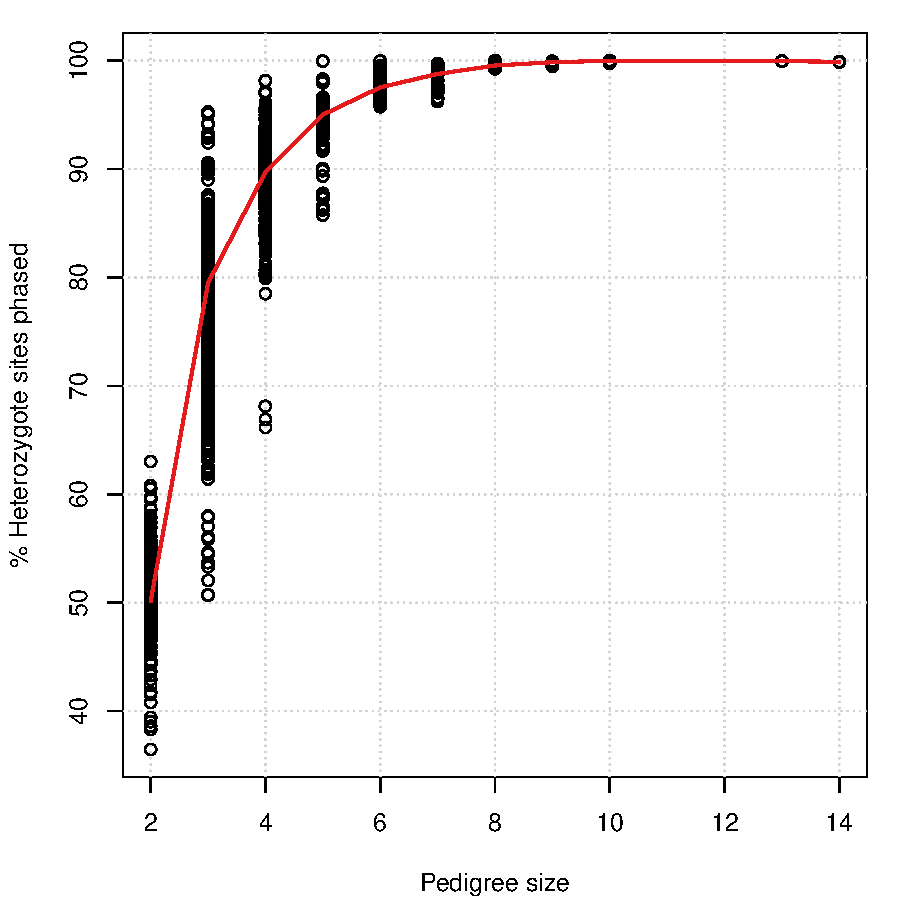
\includegraphics[width=.5\textwidth]{chap4figs/merlin_callrate}%\vspace{-20pt}
\caption[Proportion of sites phased by Merlin]{The proportion of heterozygote sites phased by Merlin against the size of the pedigree (all cohorts).  Note pedigrees of the same size may have different structures.  For example some pedigrees of size three are a parent and two children (as opposed to a mother-father-child trio).\label{fig:merlin_yield}}
\end{SCfigure}


\begin{figure}[p]
\begin{center} 
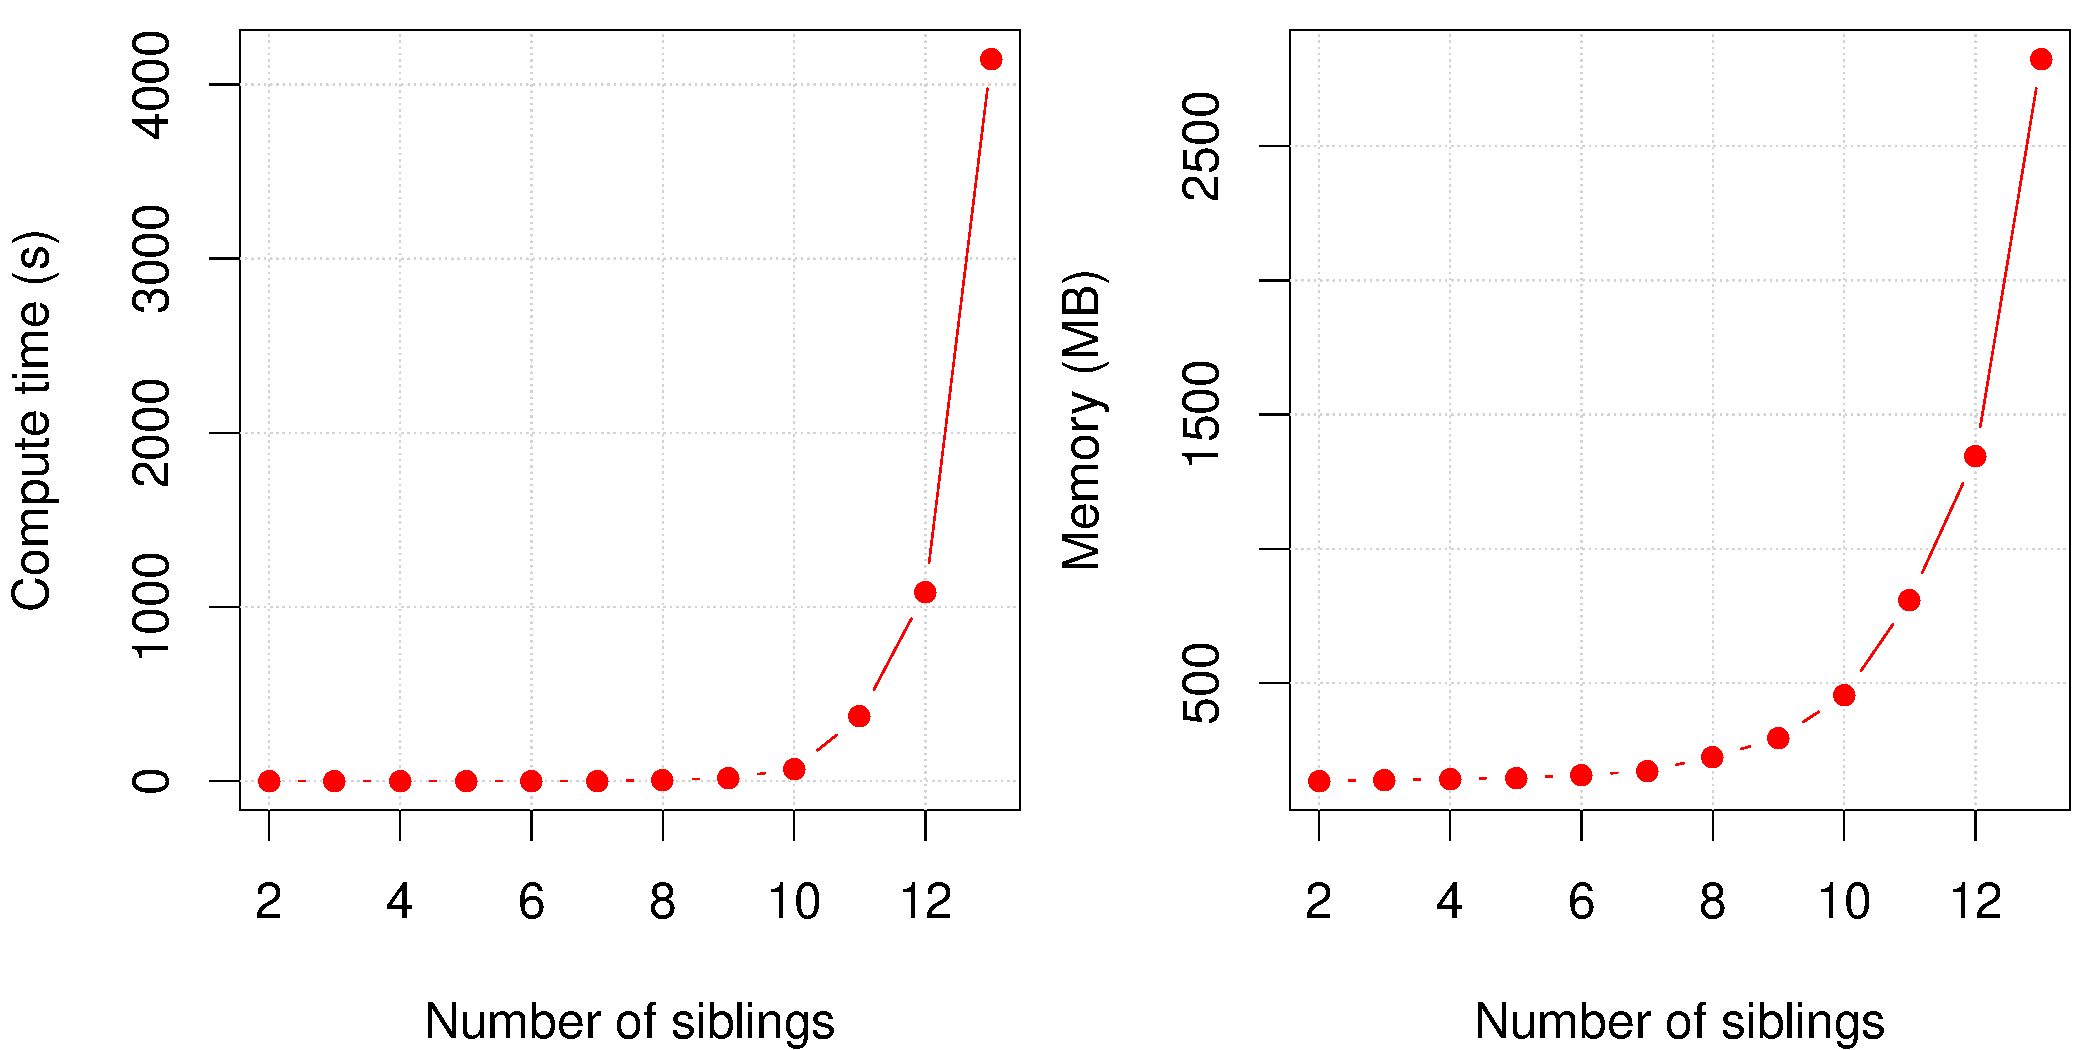
\includegraphics[width=\textwidth]{chap4figs/merlin-compute}%\vspace{-20pt}
\end{center} 
\caption[Computational performance of Merlin]{Computational performance of Merlin on simulated nuclear families of increasing size.  Computation time (left) and memory usage (right) for Merlin's haplotyping routine applied to simulated nuclear families with increasing numbers of siblings assayed at 16,297 loci on chromosome 10 (Intel Xeon CPU E5-2690 2.90GHz with 256GB RAM). For pedigrees with $<12$ non-founders, Merlin's computation time is negligible  but the method will clearly become intractable for larger pedigrees.\label{fig:merlin_compute}}
\end{figure}

\clearpage
\subsubsection{Haplotype accuracy in founder individuals}
We merged the pedigree founders with individuals who were not in any pedigree for each cohort, that is, all non-founders from pedigrees were excluded.  This gave us a sample of (nominally) unrelated individuals that we phased using each of the methods.  We applied SLRP, SHAPEIT2, Beagle and HAPI-UR to these founder data sets. We then calculated the switch error (SE of the haplotype estimates of the pedigree founders, treating the Merlin haplotypes as the truth.  This evaluation pipeline is visualised in Figure~\ref{fig:phasing_schematic}.

SLRP does not produce whole chromosome haplotypes. It only phases regions of the genome where IBD sharing is detected, and can only resolve the phase of heterozygous sites when at least one of the individuals sharing IBD is homozygous at those loci. This complicates the calculation of SE between methods. We treated each of the IBD segments inferred by SLRP separately and evaluated SE within these regions. We refer to this metric as the ``within IBD SE'', using it to evaluate SLRP's performance against methods that phase every site. We also calculated the SE of the SHAPEIT2, Beagle and HAPI-UR haplotypes across the whole of chromosome 10. We also report the yield of SLRP, defined as percentage of genotypes that are phased.

\begin{figure}[h]
  \begin{center} 
   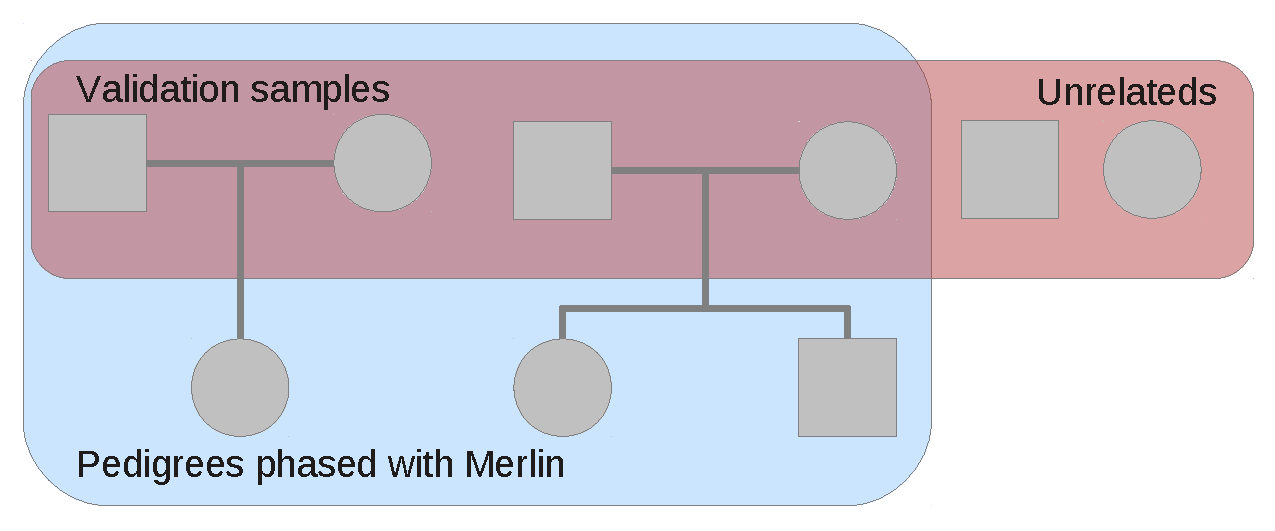
\includegraphics[width=.8\textwidth]{chap4figs/phasing_schematic}%\vspace{-20pt}
  \end{center} 
\caption[Schematic of unrelated phasing evaluation pipeline]{Schematic of unrelated phasing evaluation pipeline. This figure shows a toy example to illustrate the way in which we have used mixtures of pedigrees and unrelated samples to assess the performance of different methods. The figure shows two families of size 3 and 4 respectively and 2 unrelated samples. We used Merlin to phase the two families (blue), providing accurate haplotypes in the founders. We then ran each of the methods SHAPEIT2, Beagle and SLRP on the data from the founders and the unrelated samples (pink). The haplotypes estimated in the founder individuals was then compared to the Merlin phased haplotypes from these samples.\label{fig:phasing_schematic}}
\end{figure}


\subsubsection{Haplotype accuracy in explicitly related individuals}

Individuals in pedigrees obviously share large amounts of their genome IBD.  Algorithms that have the ability to exploit IBD sharing in distantly related individuals, may also work well on explicitly related individuals.  Hence, we also evaluated the accuracy of SHAPEIT2, SLRP, HAPI-UR and Beagle applied to the full cohorts described here, with the full extended pedigrees included.  We ran each of the methods using \emph{no} information regarding relatedness of samples.  We calculated SE for each method on the haplotypes of any individual in a pedigree larger than a mother-father-child pedigree, using the Merlin haplotypes as truth. 

SHAPEIT2, Beagle and HAPI-UR all provide functionality to phase parent-child duos and mother-father-child trios, by constraining the possible haplotypes to those consistent with the \emph{transmitted} and \emph{untransmitted} haplotypes of each parent (the child having each of the parents' transmitted haplotypes).  This approach should produce very accurate haplotypes although will return the recombined haplotypes for each parent, rather than the true parental haplotypes.  Since only several recombinations occur per chromosome, this is not introducing a substantial amount of error in the context of pre-phasing/imputation but is obviously problematic for researchers wishing to study recombination.  

Larger pedigrees could be divided into subsets of duos and trios but often there will exist no subdivision that allows all samples to exploit a parental relationship.  For example, a family with two parents and two siblings may be divided into two duos, but partitioning a nuclear family with three children means at least one child will be phased without using parental information. There is no obvious optimum way to partition pedigrees of arbitrary size and structure. We investigated a simple method where we enumerate every possible partitioning of a pedigree into duos/trios and choose the partition that minimises the number of individuals that are not included in a duo/trio (many partitions often share the same minimum in which case one is picked at random).  We applied this partitioning to the datasets and then ran Beagle (since it was the next most competitive method) taking the implied duo and trio information into account. We refer to this as the Beagle duo/trio method.  

On duos and trios this method will agree perfectly with  Merlin at sites that Merlin can phase. This introduces a possible confounding effect when using the Merlin haplotypes as the truth, as any errors in the Merlin haplotypes will not be detectable when compared to the Beagle duo/trio method. We show below using simulated data that Merlin is quite sensitive to genotyping error and that this does result in elevated switch errors. For this reason we only consider pedigrees that are more complex than a parent-child duo or father-mother-child trio when comparing methods. Larger pedigrees also give Merlin better ability to remove genotyping errors yielding more accurate validation haplotypes.


\subsubsection{Using detected recombinations for association scans of hotspot usage}
To demonstrate the utility of our recombination detection method we conducted association testing between genetic variants in the \emph{PRDM9} region (chr5:23007723-24028706)  and the ``hotspot usage'' phenotype described in \cite{coop2008high}.  Substantial association in this region was also found in \cite{kong2008detection} and \cite{hinch2011landscape}.  We calculated the same phenotype as \cite{coop2008high}, the proportion of crossover events, $\alpha_i$, that occur in a recombination hotspot for individual (the parent) $i$. This value was corrected for the probability that events occur in one of these hotspot regions by chance via simulation.  

The accuracy with which $\alpha_i$ is measured increases with the number of crossovers observed for that parent, hence parents with more observed crossovers should be given higher weighting (large nuclear families are advantageous in this situation).  We weighted individuals by creating pseudo-counts of hotspot events $k_i = n_i \times \alpha_i$ where $n_i$ is the number of crossover events observed for parent $i$.   We then fit a standard Binomial Generalised Linear Model (GLM) with $(k_i,n_i)$ as the response and the genetic dosage at each SNP as the covariate. We then performed a likelihood ratio test between this model of association and the `null' model where no genetic variant is included. Variants were imputed from the 1000 Genomes March 2012 reference panel and filtered such that all variants had MAF>0.01 and INFO>0.4 in all cohorts.

The use of the Binomial GLM allows us to leverage parents who are part of a typically uninformative meioses, where it is unlikely the majority of crossover events were detected, such individuals are simply down weighted in our association testing. 


\subsection{Simulation study}
 
In our experiments using real data we use haplotypes inferred by Merlin as the `truth' haplotypes for our methods comparison. In the Results section we show that SHAPEIT2 phases extended pedigrees with close to perfect concordance  with the Merlin haplotypes produced by Merlin (typically < 0.1\% average SE).  This level of discordance is of a similar order to both the number of recombination events, and genotyping error~\citep{oconnell2012} which the Lander-Green algorithm is known to be sensitive to.  Whilst we have applied standard quality control procedures (including Merlin's error checking) to these data, genotyping errors are likely to still be present hence at least some of this discordance may be in fact due to errors in Merlin haplotypes.  We also compare the recombination events detected by Merlin in extended families to those detected by our duoHMM approach. Any discordance between these two methods may also be due to errors in the Merlin calls.  We also wanted to investigate the ability of our method to call crossover events in duos and trios which cannot be done with the Lander-Green algorithm. For these reasons we created several simulated datasets to investigate these issues.

We utilised male chromosome X haplotypes as the basis for these simulated datasets. Since males only have one copy of chromosome X, phase is unambiguously known. As in previous phasing studies ~\citep{Lin:2002hh, browning2007, delaneau2013}, two male X chromosomes were combined to create a pseudo autosomal diploid founder individual where the true underlying haplotypes are known. We then randomly mate these new diploid individuals to produce offspring with recombined haplotypes. Crossover events were simulated as a Poisson process on the genetic lengths from the HapMap Chromosome X genetic map for females and the same map scaled by 0.605 for males, this ratio was taken from the 2002 DeCODE study where sex specific genetic lengths were reported~\cite{kong2002}.

In all experiments, we applied a simple rejection sampling scheme to avoid large amounts of consanguinity in our new diploid individuals and their offspring. The X chromosomes used to create pedigree founders were sampled such that no pair of chromosomes came from pairs of males with genome wide relatedness $r > 0.01$~\citep{hayes2009increased}. We conducted these experiments using the 1071 (607 females and 464 males) nominally unrelated individuals from the Val Borbera cohort.  This allowed use to create up 232 to diploid individuals with known haplotypes.

\subsubsection{A simulated dataset with extended pedigrees}
\label{chap4:pedsim1}
We wished to investigate accuracy on pedigrees that are collected as parts of a larger cohort, hence we simulated pedigrees with the same structures as those observed in the Val Borbera cohort.  We only used those pedigrees having ``informative'' meioses ($>3$ siblings or three generations) and generated founder individuals using male X chromosome data, these simulated founders were then ``mated'' to create descendants (and the descendants were also mated in cases of three generation pedigrees).  There were 65 such pedigrees, with 199 founders although only 108 of these founders were assayed. We carried out two sets of simulations: one realistic scenario where we attempt to emulate the type of data collected in practice and one ideal scenario which should be advantageous for Merlin.  

In the realistic scenario we simulated genotyping errors based on the confusion matrix (Table~\ref{tab:confusion_matrix}) from the genotype calling results in Chapter 2, that was estimated by comparing genotypes called on both an Affymetrix Axiom chip and a Illumina Omni 2.5S chip (GenTrain2 calls after filtering)  on 1000 Genomes individuals. There were many cases where founders were missing in practice, that is, only one parent was genotyped.  To make things as realistic as possible, we also removed the 91 unassayed founders leaving 108 assayed founders and a total of 314 individuals in pedigrees.  Finally these extended pedigrees were merged with the  607 female chromosome X data (and the remaining 33 pseudo-autosomal males not in a pedigree) to create a cohort of 954 individuals containing 314 individuals in pedigrees and 640 unrelated individuals. We created 10 versions of this simulated dataset. In the ideal scenario we do not add any genotyping error and do not remove founders (leaving all 199 founders in the data giving us a data set with 1045 individuals (405 within a pedigree).

We use the realistic dataset to compare three different versions of our method for phasing extended pedigrees. First we applied SHAPEIT2 ignoring all pedigree information. Secondly, we applied our duoHMM method to this set of haplotypes to correct SEs. We also used the duoHMM output to identify positions where there was strong evidence of genotyping error, and we investigate the effect of excluding these sites for accuracy comparisons. Finally, we applied our method of partitioning the extended pedigrees into trios and duos and then ran Beagle using this level of family information.  We also evaluate Merlin's haplotype accuracy on this simulated data.

We also ran Merlin and our duoHMM method on these datasets to detect recombination events on all informative meioses which allowed us to investigate sensitivity and specificity of the methods in both a realistic and ideal scenario. In the realistic and ideal simulation simulations, there were 183 and 212 informative meioses containing a total of 2422 and 3131 crossover events (across all simulations) on which to evaluate accuracy.
 
\begin{table}[h]
        \vspace{20pt}        
\centering
\begin{tabular}{|c|l|rrrr|}
  \hline
  &  &\multicolumn{4}{c|}{Observed genotype}\\
  &  & AA & AB & BB & Missing \\ 
  \hline
  \multirow{3}{*}{True genotype} & AA & 99.69100 & 0.04764 & 0.01286 & 0.24850 \\ 
  & AB & 0.24437 & 99.35964 & 0.12842 & 0.26757 \\ 
  & BB & 0.04536 & 0.11429 & 99.56244 & 0.27791 \\ 
   \hline
\end{tabular}
\caption[Genotype error model used in our simulations]{The genotype confusion matrix used to simulate genotyping errors in our simulation studies. This is based on the discordance between Illumina Omni2.5S (after quality control filtering) and Affymetrix Axiom chips on 1000 Genomes individuals. We took the Axiom genotypes as ``truth'' but halved the discordance and normalised the diagonal appropriately (the missing rate was left unchanged). This is to account for discordance that was actually due to Axiom chip errors. \label{tab:confusion_matrix}}
\end{table}

\subsubsection{A simulated dataset of uninformative duos}

The ability to detect recombination events is enhanced if an individual is part of a large pedigree. Such pedigrees will contain parent-child relationships where the parent's heterozygous sites can be phased independently of that child's loci (such as from a grandparent or another child) this allows changes in the pattern of inheritance (recombination events) to be detected. Previous work on detecting recombination events in pedigrees have used such informative pedigrees~\citep{coop2008high,kong2002,matise2007second,hinch2011landscape}. We wanted to assess the power of our method to detect recombination events in uninformative duos. 

We created a simulated dataset of 116 mother-father-child trios using the 464 chromosome X haplotypes from the Val Borbera cohort. These trios were merged with the diploid female chromosome X data to increase sample size. We created a second version of this simulated dataset by first removing all individuals from the Val Borbera dataset that had a genome wide relatedness $r>0.35$. This reduced the dataset from 1071 to 778 individuals (440 females and 338 males) allowing us to simulate a dataset with 84 mother-father-child trios, merged together with the original 440 females. By removing closely related individuals from the cohort we create a simulated dataset more like a non-isolated population. Detection of recombination events will be harder in this setting due to reduced levels of IBD sharing.

The merging, mating and recombination was simulated ten times (each simulation analysed separately) creating 2270 and 3190 recombination events to evaluate sensitivity and specificity of our method. We then attempted to detect the recombination events using the pipeline previously described in the previous chapter.


\section{Results}

\subsection{Levels of relatedness within each cohort}
Figure~\ref{fig:ibd_summary} (left) shows the proportion of heterozygote sites phased by SLRP, which we call the yield. SLRP's yield ranged from 31.82\% for the Split cohort to 88.15\% for the ORCADES cohort.  Split was the only cohort with less than 60\% yield demonstrating low levels of  IBD sharing between individuals in these cohorts. Following \cite{palin2011identity} we also examined individuals who were not ``closely'' related by excluding all individuals with a realised relatedness~\citep{hayes2009increased} of $r>0.125$. We found the yield was substantially lower in the CARL and FVG cohorts demonstrating some of the IBD sharing present was between closely related individuals rather than distant cousins in these cohorts. All the other cohorts did not exhibit as large a drop in yield after removing closely related individuals, highlighting the  large amounts of IBD sharing between more distantly related individuals in these cohorts. 
\vspace{10pt}
\begin{figure}[h]
 \begin{center} 
  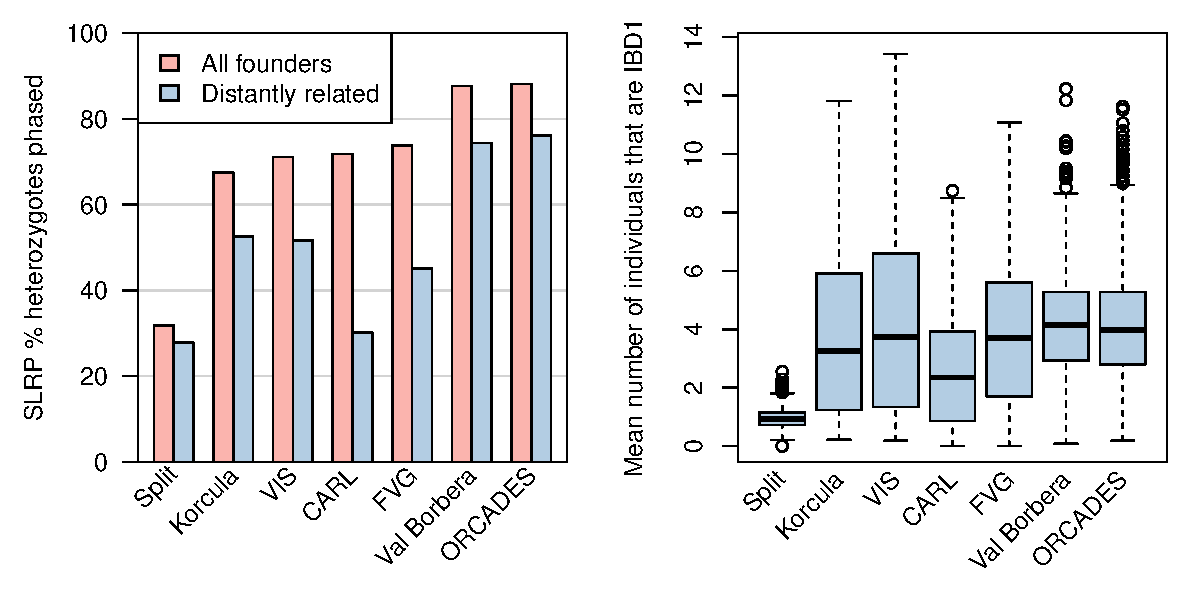
\includegraphics[width=\textwidth]{chap4figs/ibd_summary}
   \caption[ Summary of IBD sharing in cohorts]{ Summary of IBD sharing in cohorts.  \textbf{Left:} The proportion of heterozygote sites phased by SLRP for all individuals (pink) and when individuals with close relatives ($r>0.125$) are removed (blue). \textbf{Right:} The distributions of the average number  of ``surrogate'' parents for each cohort when closely related pairs ($r>0.125$) are removed.\label{fig:ibd_summary}}
 \end{center} 
\end{figure}
\clearpage
Similar to \cite{kong2008detection}, we took each individual in turn and at each locus we calculated the number of other individuals that share an IBD segment (exclude closely related individuals with relatedness $r>0.125$). We then took the average across all loci on chromosome 10 for each individual and plotted the distribution of this average IBD sharing in Figure~\ref{fig:ibd_summary} (right). The average IBD sharing is a function of both the sample size and the amount of relatedness between individuals in the population. Split again clearly has very small amounts of IBD sharing whilst the other cohorts have broadly similar distributions. It is notable that all cohorts have some individuals with $<$ 1 surrogate parent on average and some individuals in some cohorts have $>$ 10 surrogate parents. 

\subsection{Haplotype accuracy in founder individuals}
 Table~\ref{tab:switch_tab1} shows the SE rates for SHAPEIT2, SLRP, Beagle and HAPI-UR when run on the founder individuals of each cohort, both within and outside SLRP IBD segments. SHAPEIT2 consistently produced the most accurate haplotypes of all methods within IBD regions. SHAPEIT2 had a mean SE rate of between 0.14\% (ORCADES) and 0.75\% (CARL), the next closest method was SLRP with SE rates between 0.33\% (ORC/VB) and 1.99\% (Split). The next best method is Beagle with SE rates between 0.94\% (ORC) and 4.38\% (Split).  HAPI-UR has high SE rates ranging between 1.93\% (VB) and 8.30\% (Split).  It is interesting that the CARL cohort consistently has high SE rates, despite the high degree of relatedness relatedness between founders (Figure~\ref{fig:ibd_summary} (right)). Figure~\ref{fig:vb_ibd_switch} (left) shows the SLRP IBD SE rate against the SHAPEIT2 rate for each individual in the Val Borbera cohort. This highlights that while both methods produce SE rates close to zero on most individuals, SHAPEIT2 is more accurate. 
 
When calculating SE rate across the whole of chromosome 10 (not just in IBD regions), SHAPEIT2 also has the lowest error rate, ranging from 0.49\% (ORC) to 2.85\% (CARL cohort) opposed to 1.78\% and 5.57\% for Beagle and 4.20\% and 11.10\% for HAPI-UR. Switch error rates for SLRP cannot be evaluated across the whole of chromosome 10 due to the method only producing partially phased haplotypes.  We observe that \emph{all} the methods perform relatively better within IBD regions than across the whole chromosome. However, the difference for SHAPEIT2 is much larger than for Beagle and HAPI-UR. These results suggest that whilst none of these methods explicitly model IBD sharing, its presence tends to be exploited implicitly, and particularly so in SHAPEIT2. Figure~\ref{fig:vb_ibd_switch} (right)  plots the SHAPEIT2 SE rate \emph{within} IBD regions (detected by SLRP) against the rate \emph{outside} these regions. Switch error is clearly close to zero when IBD sharing is present and has a rate more comparable to outbred populations when no IBD sharing is present.
\begin{table}[h]
 \vspace{20pt}
  \begin{center}
  \resizebox{\textwidth}{!}{
    \begin{tabular}{|l|rrrrrrr|}
      \hline
      Cohort  & CARL & FVG & KOR & ORC & SPL & VB  & VIS \\ 
      Chip  & 370K & 370K  &  370K & 300K & 370K & 370K & 300K \\
      \hline
      N validation individuals & 130 & 274  & 118 & 201 & 50 & 481 & 150 \\
      \hline
      SLRP Yield & 71.82 & 73.82  & 67.52 & 88.15 & 31.82 & 87.63 & 71.09 \\ 
      \hline
      SHAPEIT2 (IBD) & 0.75 & 0.21  & 0.18 & 0.14 & 0.60 & 0.17 & 0.19 \\ 
      SLRP (IBD) & 1.15 & 0.40 &  0.45 & 0.33 & 1.99 & 0.33 & 0.43 \\ 
      Beagle (IBD) & 2.57 & 1.18  & 1.25 & 0.94 & 4.38 & 1.07 & 1.30 \\ 
      HAPI-UR 3x (IBD) & 5.43 & 2.25  & 2.55 & 2.59 & 8.30 & 1.93 & 2.94 \\ 
      \hline
      SHAPEIT2 (No IBD) & 5.03 & 4.10  & 3.11 & 2.43 & 3.35 & 2.74 & 3.65 \\ 
      Beagle (No IBD) & 7.73 & 5.72  & 5.55 & 5.05 & 6.00 & 5.03 & 6.36 \\ 
      HAPI-UR 3x (No IBD) & 15.97 & 10.31  & 10.20 & 9.94 & 12.09 & 7.92 & 12.47 \\ 
      \hline
      SHAPEIT2 & 2.85 & 1.81  & 1.05 & 0.49 & 2.65 & 0.62 & 1.16 \\ 
      Beagle & 5.31 & 3.11  & 2.53 & 1.78 & 5.57 & 1.88 & 2.78 \\ 
      HAPI-UR 3x & 11.21 & 5.83  & 4.82 & 4.20 & 11.10 & 3.21 & 5.77 \\ 
      \hline
    \end{tabular}
    }
    \caption[Phasing accuracy in nominally unrelated individuals]{Switch error rates for samples containing nominally unrelated individuals.  All individuals not explicitly related in the defined pedigrees were phased.  We calculate overall SE rate (All), for chromosome 10 (this is not possible for SLRP) as       well as SE rates within(IBD) and outside (no IBD) SLRP detected IBD regions. SHAPEIT2 consistently produces the most accurate haplotypes. \textbf{Chip abbreviations:} 370K - Illumina HumanHap 370CNV. 300K - Illumina HumanHap 300, 2.5S - Illumina Omni 2.5S. \label{tab:switch_tab1}}
  \end{center}
\end{table}
\newpage
\begin{figure}[h]
  \begin{center} 
   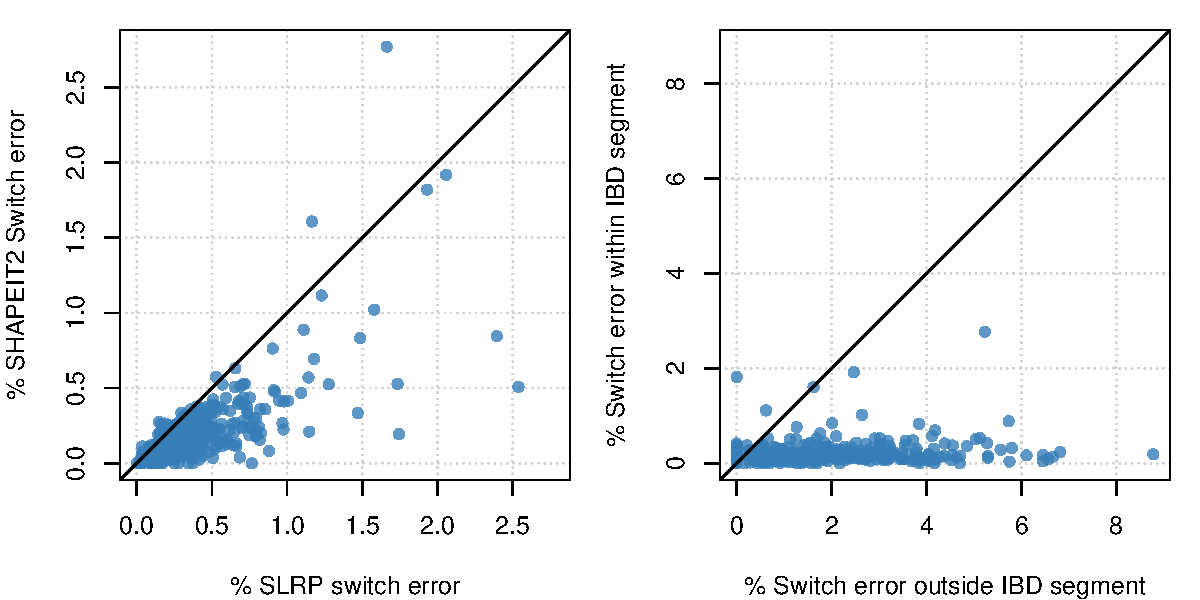
\includegraphics[width=\textwidth]{chap4figs/vb_switcherror}%\vspace{-20pt}    
  \end{center} 
  \caption[SHAPEIT2 and SLRP accuracy in IBD regions]{Evaluation of SHAPEIT2 and SLRP accuracy in IBD regions for the Val Borbera cohort. \textbf{Left:} The SHAPEIT2 switch error rates (within IBD regions) against the SLRP rates for each founder individual in the Val Borbera cohort.  Both methods achieve low error rates but SHAPEIT2 has lower rates for most individuals. \textbf{Right:} The switch error rate for SHAPEIT2 \emph{within}  SLRP IBD regions against the rate \emph{outside} SLRP IBD regions.  Haplotypes are far more accurate when IBD sharing is present.\label{fig:vb_ibd_switch}}
\end{figure}

\subsection{Haplotype accuracy in extended pedigrees}

\subsubsection{Treating all individuals as unrelated}

Table~\ref{tab:switch_tab2} shows the SE rates for SHAPEIT2, SLRP, Beagle and HAPI-UR when run on all individuals in each cohort and ignoring any of the information about explicit family relationships between individuals. We calculated SE for each method on the haplotypes of any individual within an extended pedigree more complex than a simple duo or trio, using the Merlin haplotypes as truth. All of the methods have lower SE rates than when run on just the founders of the pedigrees (Table~\ref{tab:switch_tab1}) but the improvement for SHAPEIT2 is most striking. We find that SHAPEIT2 achieves between 0.059 \% (Korcula) and 0.241 \% (CARL) SE rate on individuals within pedigrees.  SLRP achieves a very high yield in most cohorts ($>90$\% except in Split)  for individuals within pedigrees and improved accuracy within the IBD regions it detects.  Both Beagle and HAPI-UR (3X) are also more accurate in this setting as well but do not obtain the same gains as SHAPEIT2. 


\begin{table}[h]
        \vspace{20pt}        
\begin{center}
\resizebox{\textwidth}{!}{
  \begin{tabular}{|l|rrrrrrr|}
  \hline
   Cohort  & CARL & FVG  & KOR & ORC & SPL & VB  & VIS \\ 
   Chip  & 370K & 370K   & 370K & 300K & 370K & 370K & 300K \\
  \hline
   N validation individuals & 228 & 460 & 118 & 300 & 38 & 739 & 154 \\ 
   \hline
   SLRP Yield & 90.870 & 96.094 & 96.319 & 98.344 & 81.523 & 98.613 & 97.818 \\ 
  \hline
  SHAPEIT2 (IBD) & 0.209 & 0.086  & 0.058 & 0.066 & 0.090 & 0.073 & 0.075 \\ 
  SLRP (IBD) & 0.683 & 0.319  & 0.486 & 0.301 & 1.075 & 0.387 & 0.116 \\ 
  Beagle (IBD) & 1.211 & 0.825 & 0.970 & 0.353 & 4.073 & 0.492 & 0.923 \\ 
  HAPI-UR 3x (IBD) & 2.773 & 1.445 & 1.755 & 1.072 & 7.599 & 0.860 & 1.952 \\ 
  \hline
  SHAPEIT2 (No IBD) & 0.768 & 0.424  & 0.105 & 1.217 & 0.112 & 0.423 & 0.162 \\ 
  Beagle (No IBD) & 3.893 & 3.338  & 3.211 & 3.741 & 4.293 & 2.462 & 3.673 \\ 
  HAPI-UR 3x (No IBD) & 8.150 & 5.698  & 6.186 & 5.898 & 8.747 & 3.544 & 7.233 \\ 
  \hline
  SHAPEIT2 & 0.241 & 0.097  & 0.059 & 0.083 & 0.093 & 0.078 & 0.076 \\ 
  Beagle & 1.362 & 0.907  & 1.034 & 0.403 & 4.096 & 0.516 & 0.973 \\ 
  HAPI-UR 3x & 3.074 & 1.582  & 1.880 & 1.141 & 7.722 & 0.892 & 2.049 \\ 
  \hline  \hline
  SHAPEIT2+duoHMM & 0.232 & 0.092  & 0.058 & 0.079 & 0.091 & 0.073 & 0.073 \\ 
  Beagle+duoHMM & 0.934 & 0.643  & 0.789 & 0.255 & 3.200 & 0.318 & 0.703 \\ 
  HAPI-UR+duoHMM 3x & 2.134 & 1.108  & 1.415 & 0.640 & 6.193 & 0.502 & 1.494 \\ 
  \hline
%  Duo\_Trio SHAPEIT2 & 0.206 & 0.113 & - & 0.046 & 0.082 & 0.044 & 0.067 & 0.078 \\ 
  Beagle Duo/Trio & 0.445 & 0.265  & 0.113 & 0.151 & 0.595 & 0.175 & 0.129 \\ 
  \hline
  \hline
  Masked SHAPEIT2+duoHMM & 0.088 & 0.056   & 0.047 & 0.052 & 0.060 & 0.045 & 0.060 \\ 
  Masked  Beagle Duo/Trio & 0.360 & 0.238 & 0.111 & 0.146 & 0.584 & 0.165 & 0.127 \\ 
  \hline
  \end{tabular}
}

\caption[Switch error rates in large pedigrees]{Switch error (SE) rates for different methods applied to extended pedigrees.  We evaluate SE for individuals who are members of a complex pedigree (pedigrees that are larger than a parent-child duo and father-mother-child trio). The first row is the number of individuals from each cohort in such pedigrees.  The second row shows the yield of SLRP when applied to each cohort. Rows 3-7 show the SE for SHAPEIT2, SLRP, Beagle and HAPI-UR within SLRP detected IBD regions. Rows 7-8 show the SE for SHAPEIT2, Beagle and HAPI-UR outside SLRP detected IBD regions. Rows 10-12 show the overall SE for SHAPEIT2, Beagle and HAPI-UR. Rows 13-15 show the overall SE for SHAPEIT2, Beagle and HAPI-UR haplotypes after correction with the duoHMM method. Row 16 show the overall SE for  Beagle applied to pedigrees partitioned into duos and trios where possible. Rows 17-18 show the switch error rate for the SHAPEIT2+duoHMM and Beagle Duo/Trio phasing \emph{after} masking genotypes flagged as erroneous by the duoHMM.\label{tab:switch_tab2}}
\end{center}
\end{table}

 \subsubsection{duoHMM corrected haplotypes}
We applied our duoHMM method to the SHAPEIT2, Beagle and HAPI-UR haplotypes that were estimated ignoring all family information. To give a sense of the output of applying this model Figure~\ref{fig:duo_hmm}  shows the Viterbi paths of 50 male parent duos from the Val Borbera cohort for both SHAPEIT2 and Beagle. The four possible IBT states $(A,B,C,D)$ are shown using colours pale blue, dark blue, light red and dark red respectively. Changes between a blue and red colour correspond to a $T_3$ or $T_4$ transition, both of which imply a SE in the child. Changes of colour between light and dark blue or between light and dark red correspond to $T_2$ transitions, which correspond to a change on IBT state in the parent, and could be caused by a recombination or a SE in the parent. Figure~\ref{fig:duo_hmm_examples} provides examples that can be helpful in interpreting Figure~\ref{fig:duo_hmm}. 

Figure~\ref{fig:duo_hmm} shows a striking difference between the output on the SHAPEIT2 and Beagle haplotypes. The SHAPEIT2 paths have very few transitions of all types, and when transitions occur they are predominantly $T_2$ transitions. The figure shows only father-child duos and chromosome 10 has been estimated to have a genetic length 1.34 Morgans for paternal meioses~\citep{kong2002}. The numbers of $T_2$ transitions in the 50 duos in Figure~\ref{fig:duo_hmm} looks reasonably consistent with this genetic length, suggesting that the $T_2$ transitions are indeed true recombination events. We note that there are some duos with no transitions. This is a possible outcome of a meiosis and is more likely to occur on the shorter chromosomes and can also be the product of an undetected recombination event.

The Beagle haplotypes contain many more $T_2$, $T_3$ and $T_4$ transitions. In the Val Borbera cohort when we compared the SHAPEIT2 and Beagle haplotypes to those estimated by Merlin we found that SHAPEIT2 produced 4,613 SEs in 1,074 individuals corresponding to 4.3 switches per individual, whereas Beagle produced 29,681 switches or 27.6 switches per individual. These numbers seem consistent with what we observe in Figure~\ref{fig:duo_hmm}. The higher rate of SEs in the Beagle haplotypes cause a large number of changes in estimated IBT state.

\begin{figure}[p]
 \begin{center} 
  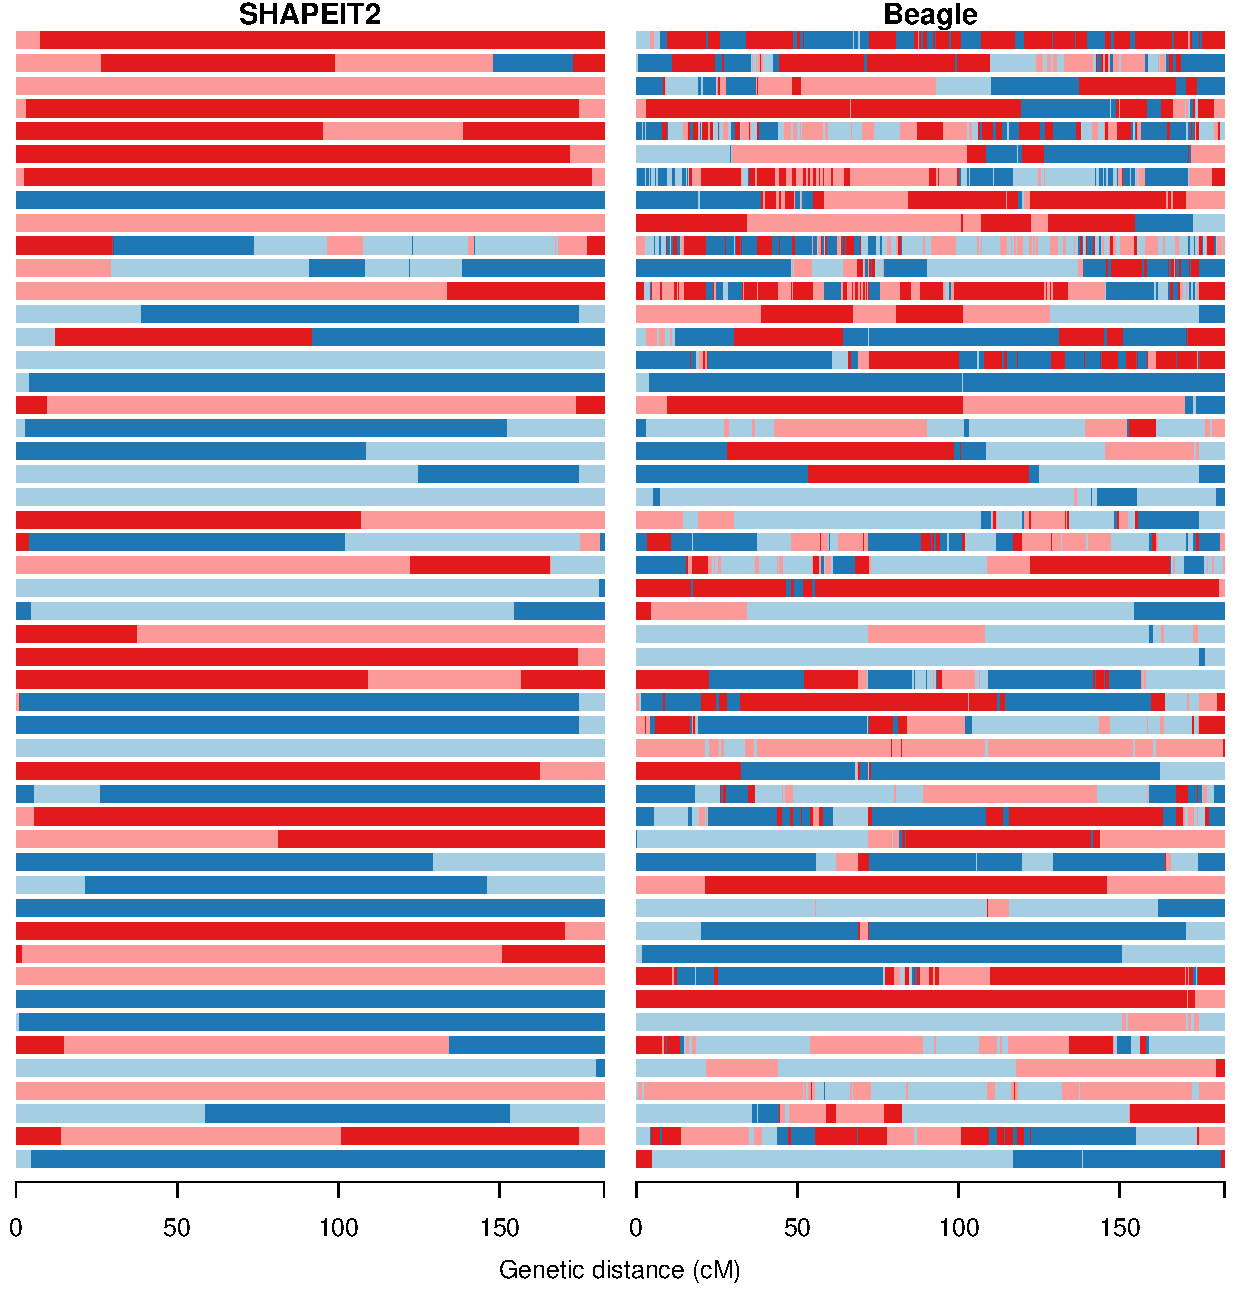
\includegraphics[width=\textwidth]{chap4figs/valborbera_b37-paternal}
   \caption[Observed DuoHMM paths in real data]{The DuoHMM Viterbi paths for 50 father-child duos from the Val Borbera cohort on chromosome 10. The four possible IBT states (A, B, C, D) are shown using colours pale blue, dark blue, light red and dark red respectively. The left and right panels show the results of the duo HMM applied to the SHAPEIT2 and Beagle haplotypes respectively. Changes between a blue and red colour correspond to a $T_3$ or $T_4$ transition, both of which imply a SE in the child. Changes of colour between light and dark blue or between light and dark red correspond to $T_2$ transitions, which correspond to a change on IBT state in the parent, and could be caused by a recombination or a SE in the parent. The x-axis shows the sex-averaged genetic distance across the chromosome in centiMorgans. \label{fig:duo_hmm}}
 \end{center} 
\end{figure}

Table~\ref{tab:pedtab1} shows the mean number of state transitions in paternal and maternal duos for each cohort for SHAPEIT2 and Beagle.  Note that $T_3$ and $T_4$ transitions are biologically impossible as they represent a change in which child haplotype the parent is transmitting genetic material to.  The SHAPEIT2 haplotypes have $<0.5$ of these transitions occurring per duo in all cohorts whilst Beagle ranges from 7.49 to 97.17 for $T_3$ transitions. 

\begin{table}
        \vspace{20pt}        
\begin{center}
\resizebox{\textwidth}{!}{
\begin{tabular}{|l|cc||ccc|ccc||ccc|ccc|}
  \hline
  &  &  & \multicolumn{6}{c||}{SHAPEIT2} & \multicolumn{6}{c|}{Beagle}\\
  \hline
  &  \multicolumn{2}{c||}{Duos}  & \multicolumn{3}{c|}{Paternal} & \multicolumn{3}{c||}{Maternal} & \multicolumn{3}{c|}{Paternal} & \multicolumn{3}{c|}{Maternal} \\
  &P&M&$T_2$&$T_3$&$T_4$&$T_2$&$T_3$&$T_4$&$T_2$&$T_3$&$T_4$&$T_2$&$T_3$&$T_4$\\
  \hline

  %%results using HapMap LD based map
  CARL & 72 & 120 & 1.47 & 0.26 & 0.00 & 2.73 & 0.72 & 0.07 & 34.35 & 24.19 & 0.83 & 50.99 & 25.09 & 1.07 \\ 
  FVG & 163 & 289 & 1.29 & 0.26 & 0.02 & 2.25 & 0.42 & 0.03 & 30.17 & 19.23 & 0.73 & 27.06 & 13.99 & 0.43 \\ 
%  GPC & 228 & 462 & 2.99 & 1.37 & 0.02 & 4.26 & 1.64 & 0.04 & 11.79 & 10.31 & 0.17 & 16.95 & 10.10 & 0.15 \\ 
  KOR & 49 & 104 & 0.71 & 0.04 & 0.00 & 1.15 & 0.00 & 0.00 & 32.84 & 24.35 & 1.24 & 42.68 & 25.52 & 1.38 \\ 
  ORC & 148 & 187 & 0.90 & 0.00 & 0.00 & 2.00 & 0.04 & 0.00 & 9.16 & 9.49 & 0.31 & 11.41 & 7.49 & 0.22 \\ 
  SPL & 18 & 35 & 0.17 & 0.00 & 0.00 & 1.20 & 0.00 & 0.00 & 122.33 & 97.17 & 6.17 & 128.20 & 88.69 & 6.54 \\ 
  VB & 303 & 479 & 1.46 & 0.31 & 0.02 & 2.25 & 0.38 & 0.05 & 13.89 & 14.82 & 0.33 & 15.35 & 13.53 & 0.32 \\ 
  VIS & 68 & 130 & 1.29 & 0.16 & 0.03 & 2.07 & 0.49 & 0.02 & 19.74 & 18.56 & 0.60 & 43.25 & 15.15 & 0.72 \\ 
  \hline
\end{tabular}
}
\end{center}
\caption[Summary of DuoHMM state transitions for each cohort]{Summary of DuoHMM state transitions for each cohort. The mean number of switches occurring (excluding $T_1$)  found by the Viterbi path through our four state HMM for SHAPEIT2 and Beagle maximum likelihood haplotypes for chromosome 10 for paternal (P) and maternal (M) duos.  SHAPEIT2 has very few impossible transmissions ($T_3$ and $T_4$) and the number possible recombinations ($T_2 + T_4$) are much closer to the genetic length of chromosome 10 than Beagle.  The 2002 deCODE map gives the chromosome 10 genetic  length as 1.34 and 2.18 Morgans for males and females respectively. \label{tab:pedtab1}}
\end{table}

Transitions $T_2$ and $T_4$ may correspond to crossover events or SEs in the parental haplotypes. The 2002 deCODE map gives the chromosome 10 genetic length as 1.34 and 2.18 Morgans for males and females respectively~\citep{kong2002}. The mean numbers of $T_2$ or $T_4$ transitions in the SHAPEIT2 show rough agreement with the expected number of recombinations on chromosome 10 in most cohorts.  For example, in the VIS cohort we observe $T_2+T_4=1.32$ and $T_2+T_4=2.09$ transitions in males and females respectively. The female rates in CARL are higher than we might expect at 2.8. Both the male and female rates are lower than we might expect in the Korcula and Split cohort.  This is likely due to insufficient information in the data to infer the true parental haplotype and hence we are seeing a parental SE at the recombination event, that is, we are inferring the \emph{transmitted} haplotypes.

Table~\ref{tab:switch_tab2} shows the mean SE rate after applying haplotype corrections. The corrections lead to a consistent but small improvement for the SHAPEIT2 haplotypes, the largest improvement was a .009\% decrease in SE for the CARL cohort.  These results further highlight the very high quality haplotype estimates that SHAPEIT2 produces even though it is ignoring all explicit pedigree information. 

We also find the duoHMM method is beneficial to Beagle and HAPI-UR when used to correct those haplotypes. For example the SE rate for HAPI-UR drops from 7.72\% to 6.19\% for the Split cohort. Table~\ref{tab:correction_table} gives the average number and type of correction applied to each cohort for each method.  SHAPEIT2's haplotypes require less than 0.5 corrections on average for chromosome 10, this is consistent with the very small improvement in SE.

\begin{table}[h]
\centering
\begin{tabular}{|l|rrr|rrr|rrr|}
  \hline
  &\multicolumn{3}{c|}{SHAPEIT2}&\multicolumn{3}{c|}{Beagle}&\multicolumn{3}{c|}{HAPI-UR 3X}\\
  \hline`
  & P & M & C & P & M & C& P & M & C\\
  \hline
  CARL & 0.010 & 0.058 & 0.010 & 1.505 & 2.507 & 0.828 & 3.461 & 5.491 & 1.576 \\ 
  FVG & 0.040 & 0.134 & 0.028 & 3.248 & 3.629 & 2.203 & 5.936 & 8.224
  & 3.818 \\ 
%  GPC & 0.118 & 0.291 & 0.096 & 0.893 & 1.769 & 0.646 & 1.216 & 2.442 & 0.917 \\ 
  KOR & 0.156 & 0.427 & 0.078 & 4.516 & 5.967 & 3.368 & 10.305 & 14.314 & 6.473 \\ 
  ORC & 0.045 & 0.038 & 0.008 & 1.816 & 1.426 & 0.531 & 6.022 & 5.201 & 2.490 \\ 
  SPL & 0.010 & 0.103 & 0.008 & 1.447 & 3.350 & 0.651 & 2.645 & 6.667 & 1.331 \\ 
  VB & 0.076 & 0.143 & 0.019 & 2.900 & 4.367 & 1.176 & 6.127 & 9.112 & 2.373 \\ 
  VIS & 0.058 & 0.200 & 0.006 & 4.378 & 7.326 & 1.092 & 7.264 & 12.404 & 1.990 \\ 
  \hline
\end{tabular}
        \caption[Average number of corrections applied to haplotypes by DuoHMM]{The average number of corrections applied to haplotypes for each method. `P' and `M' denotes when we correct a child's haplotypes using information from the paternal (P) or maternal (M) haplotypes, to ensure consistent gene flow. `C' denotes when multiple children were used to find the minimum recombinant parental haplotypes.  Very few corrections are required for the SHAPEIT2 haplotypes compared to Beagle and HAPI-UR, this is also evident from the switch error improvements shown in Table 2. It is interesting to note that maternal meioses tend to yield more corrections, this is possibly due to (assayed) mothers tending to be in larger nuclear families.\label{tab:correction_table}}

\end{table}



\subsubsection{Partitioning pedigrees into Duos/Trios}


Table~\ref{tab:switch_tab2}  also shows the haplotype accuracy for pedigrees that were partitioned into duos and trios and then phased accordingly using Beagle (denoted as Beagle Duo/Trio).  Not surprisingly, adding the duo/trio relationships yields a substantial improvement to the Beagle haplotypes across all cohorts, for example we see a drop from 1.362\% SE to 0.445\% SE in CARL. However they are still consistently less accurate than SHAPEIT2's haplotypes (even though SHAPEIT2 is not using any relationships). 

When using the Beagle Duo/Trio method some individuals will not be phased as part of a duo or trio, for example one of the children in a three sibling nuclear family. Figure~\ref{fig:trio_fig} (top and centre left) plots the SE for such ``unrelated'' individuals (for all cohorts) for Beagle Duo/Trio versus SHAPEIT2 and Beagle Duo/Trio versus SHAPEIT2+duoHMM respectively. These plots shows that these individuals are phased much more accurately using our methods. Duos and trios are phased almost equally well by all methods.

\begin{figure}
 \begin{center} 
  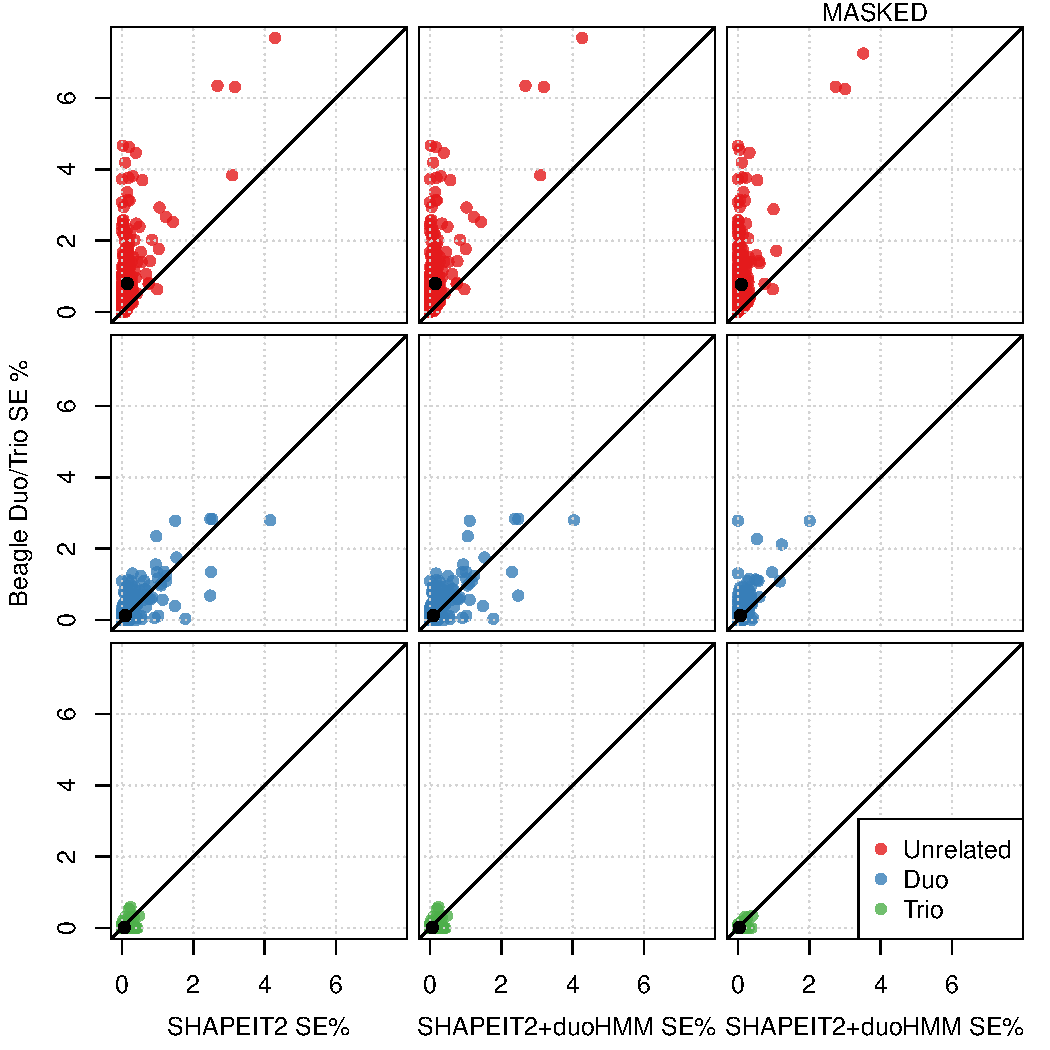
\includegraphics[width=\textwidth]{chap4figs/ALL-trio-duo-switch-3x3-v2}
   \caption[Phasing accuracy in extended pedigrees]{Switch error rates for individuals in extended pedigrees for different phasing pipelines  across all European cohorts (chromosome 10).  Points are coloured according to what relationship was used to phase that individual (red meaning no relationships were used).  \textbf{Left:}  Beagle using duo/trio phasing versus SHAPEIT2 using no relationships.  \textbf{Centre:} Beagle using duo/trio phasing versus SHAPEIT2+duoHMM using no relationships.       \textbf{Right:}  Beagle using duo/trio phasing versus SHAPEIT2+duoHMM using no relationships when masking loci flagged as probable genotyping errors by the duoHMM. Switch error is reduced for both methods suggesting the masking is sensible.
     \label{fig:trio_fig}}
 \end{center} 
\end{figure}

We used our SHAPEIT2+duoHMM method to flag sites of possible genotyping error and then re-calculated the SE rates for SHAPEIT2+duoHMM and the Beagle Duo/Trio method excluding these sites. The results are shown in the last two rows of Table~\ref{tab:switch_tab2}. Comparing these results to the unmasked results we see that the reduction in SE is greatest for SHAPEIT2+duoHMM, suggesting that genotyping error causes the results of Beagle Duo/Trio to appear better than they are. Our simulation study results described in the next subsection agree further weight to this point. Figure~\ref{fig:trio_fig} (right) shows in more detail the effect of masking our genotyping errors, and that SHAPEIT2+duoHMM outperforms Beagle Duo/Trio in unrelateds, duos and trios.  


\subsubsection{Results on the simulated dataset with extended pedigrees}

The simulated pedigree data allows us to evaluate the confounding effect of genotype errors in the Merlin and duo/trio phased haplotypes.

Figure~\ref{fig:simfig2} (top right) plots the SE of SHAPEIT2+duoHMM versus Merlin on simulated data with realistic levels of genotyping error. SHAPEIT2+duoHMM is generally more accurate (average of 0.033\% versus 0.215\% for Merlin on sites resolved by Merlin). Without any genotyping error (Figure~\ref{fig:simfig2} bottom right) the performance is much improved for Merlin (SHAPEIT2+duoHMM SE=0.005\%, Merlin=0.021\%). Overall, these results suggest that at least some of the observed discordance in the analysis of real data sets is due to errors in the Merlin haplotypes caused by genotyping error. The true error levels are likely to be lower but the masking can help to remove the confounding effect.

The SE rates of SHAPEIT2, SHAPEIT2+duoHMM and Beagle Duo/Trio were 0.104\%, 0.065\% and 0.269\% respectively. When we removed sites flagged as genotyping errors by our method the SE rates were 0.073\%, 0.034\% and 0.231\% respectively, suggesting that the masking can remove switch errors caused by genotyping errors. Figure~\ref{fig:simfig1} plots the SE rates on the simulated pedigrees for Beagle Duo/Trio SE rates of all individuals versus those of SHAPEIT2 (left) and SHAPEIT2+duoHMM (centre). The plot shows that the most accurate haplotypes are attained by the SHAPEIT2+duoHMM approach, that the duo/trio constrained phasing can be somewhat susceptible to genotyping error and that individuals that cannot be phased as a duo/trio are substantially less accurate with the Beagle approach.



\begin{figure}
  \begin{center} 
    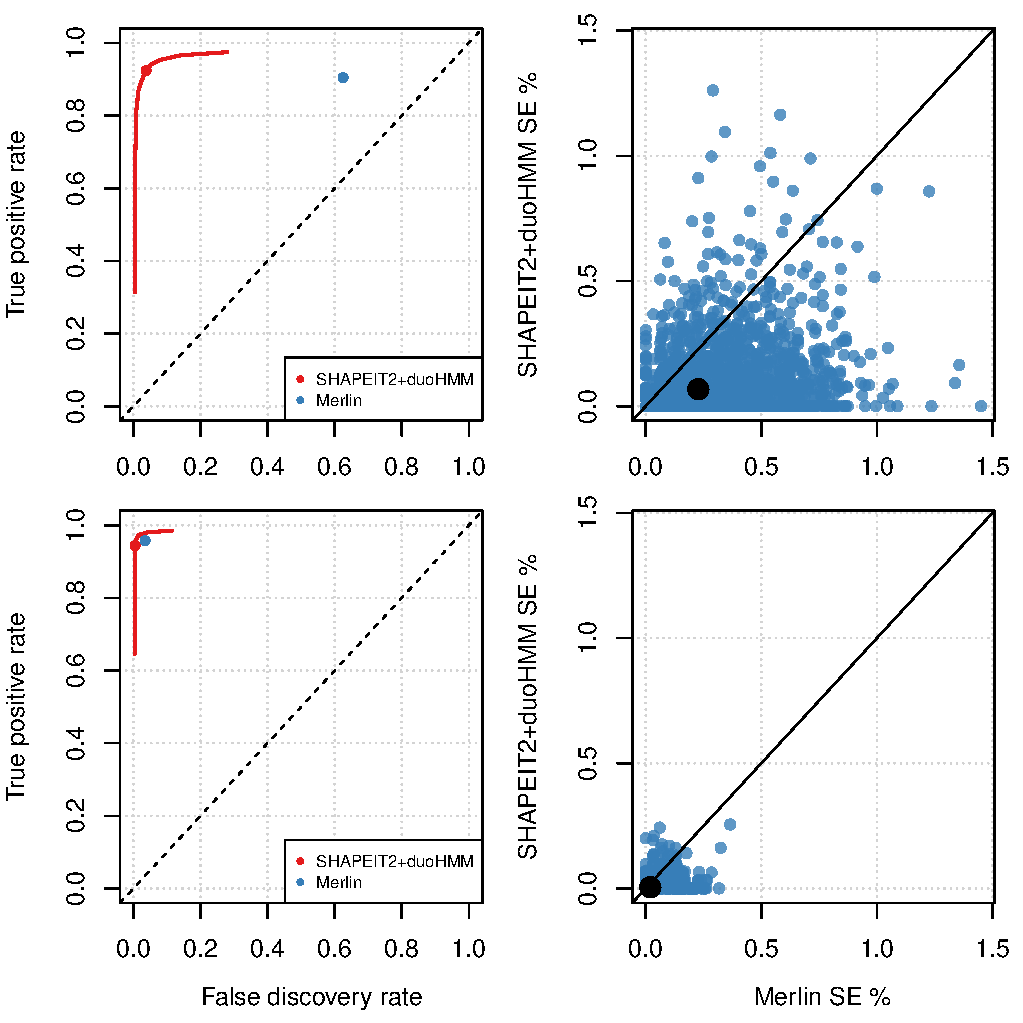
\includegraphics[width=\textwidth]{chap4figs/chrx_experiment_fullped-final.pdf}
  \end{center}
\caption[Comparison of SHAPEIT2 and Merlin on simulated pedigrees]{ Detection of recombination in simulated extended pedigrees and comparison of SHAPEIT2 and Merlin haplotype accuracy for realistic data~(top) and ideal data~(bottom). \textbf{Left:} True positive rate (TPR) versus false discovery rate (FDR) for recombination detection using SHAPEIT2+duoHMM (red) versus Merlin (blue). Merlin detects 89.93\% of crossovers with a substantial FDR of 63.48\% whilst SHAPEIT2+duoHMM detect 92.25\% of events with an FDR of 3.87\% (the red point at $P(R) > 0.5$. On ideal data SHAPEIT2+duoHMM achieve a 95.75\% TPR and 0.71\% FDR and Merlin has 95.66\% and 3.478\% respectively.  \textbf{Right:} Switch error for SHAPEIT2~(DuoHMM corrected) versus Merlin.  The black point is the mean for each method.  Merlin had  0.215\% (0.021\% ideal scenario) switch error while SHAPEIT2 had a rate of 0.033\% (0.005\% ideal scenario).
\label{fig:simfig2}}
\end{figure}


\begin{figure}
  \begin{center} 
   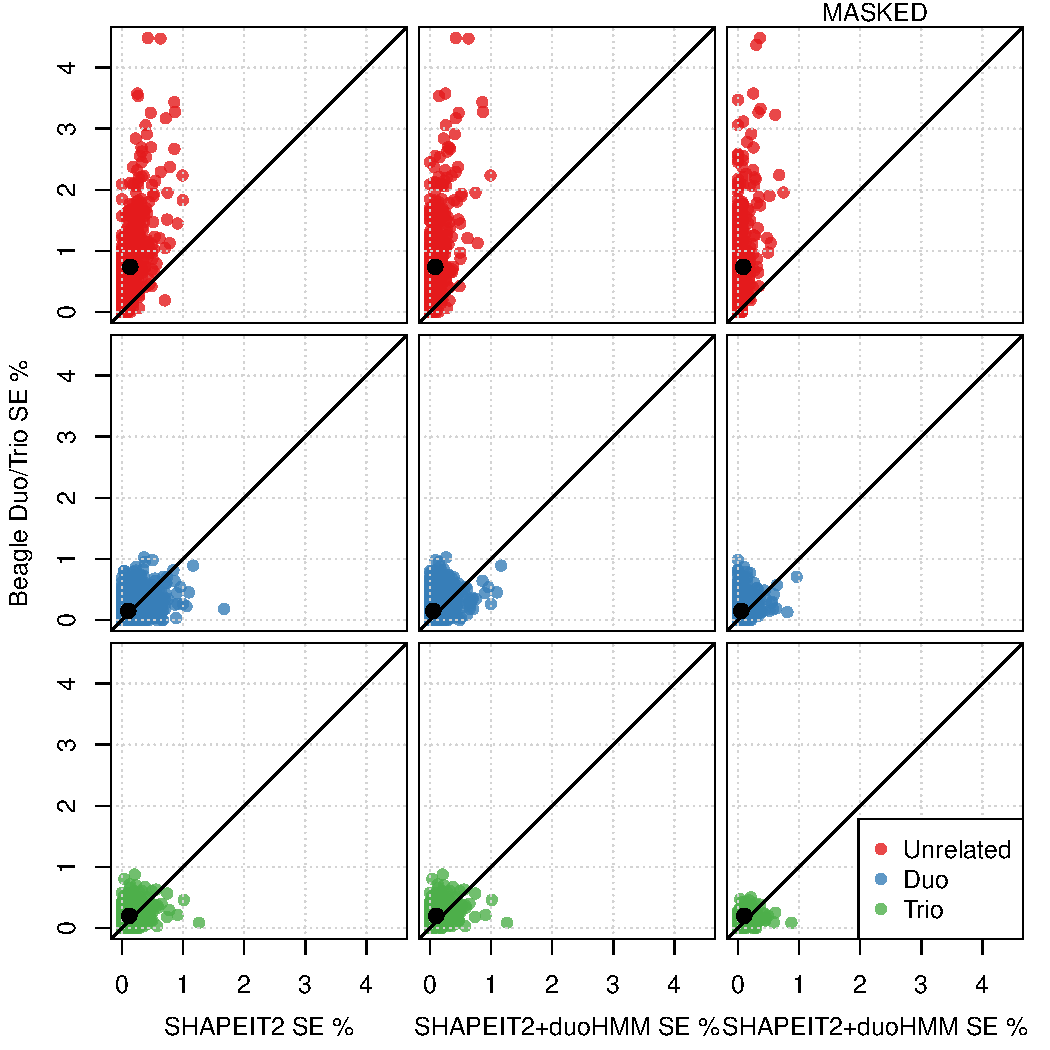
\includegraphics[width=\textwidth]{chap4figs/beagletrio_vs_s2-3x3.pdf}
  \end{center}
  \caption[Comparison of SHAPEIT2 and Beagle on simulated pedigrees]{Switch error results on simulated data for extended pedigrees.  Points are coloured according to what family information was used by Beagle in duo/trio mode; red meaning an individual could not be included in a duo or trio. \textbf{Left:} Beagle duo/trio switch error rate (0.269\% average SE) against switch error rate for SHAPEIT2 when all individuals are treated as unrelated (0.104\% average SE). \textbf{Centre:} After applying the duoHMM haplotype corrections to SHAPEIT2 (0.065\% average SE). \textbf{Right:} Switch error after  masking genotypes flagged as erroneous by the SHAPEIT2+duoHMM, Beagle duo/trio phasing is reduced to 0.231\% and SHAPEIT2+duoHMM to 0.034\%.\label{fig:simfig1}}
\end{figure}

\subsection{Detecting recombination events}

\subsubsection{Informative pedigrees}

We evaluated the sensitivity and specificity of our recombination detection routine as well as Merlin on our simulated data.  Figure~\ref{fig:simfig2} shows the true positive rate (TPR) against the false discovery rate (FPR) for 2422 realistic (3131 ideal) simulated crossover events from 1830 (2120 ideal) informative meioses.  In the simulations with realistic levels of genotyping error (Figure~\ref{fig:simfig2} top left), Merlin detects 88.2\% of events but with a substantial FPR of 63.5\% while SHAPEIT2 has a FPR of 1.94\% at the same rate of detection. SHAPEIT2 has the additional advantage of have a probability associated with each event, which can be thresholded. For example, by setting a threshold of $P(R)>0.5$ we can achieve a FPR=3.78\% and TPR=92.4\% or $P(R)>0.9$ for 0.58\% and 69.45\% respectively. In the absence of genotyping error (Figure~\ref{fig:simfig2} bottom left) the performance of Merlin is improved (FPR=3.48\% and TPR=95.66\%) but SHAPEIT2 is marginally better (FPR=0.71\% and TPR=95.75\% at $P(R)>0.5$).

Figure~\ref{fig:shapeit-merlin} compares the gene flow (and hence recombination) inferred by Merlin and the recombination probabilities inferred by our method for 10 informative meioses between parent-child duos from the Val Borbera cohort on chromosome 10. This figure shows  good agreement between our estimated probabilities and the events inferred by Merlin. However, these examples highlight that Merlin does infer some rather implausible, sporadic events in some meioses (even after running Merlin's error detection).

\begin{figure}
 \begin{center} 
  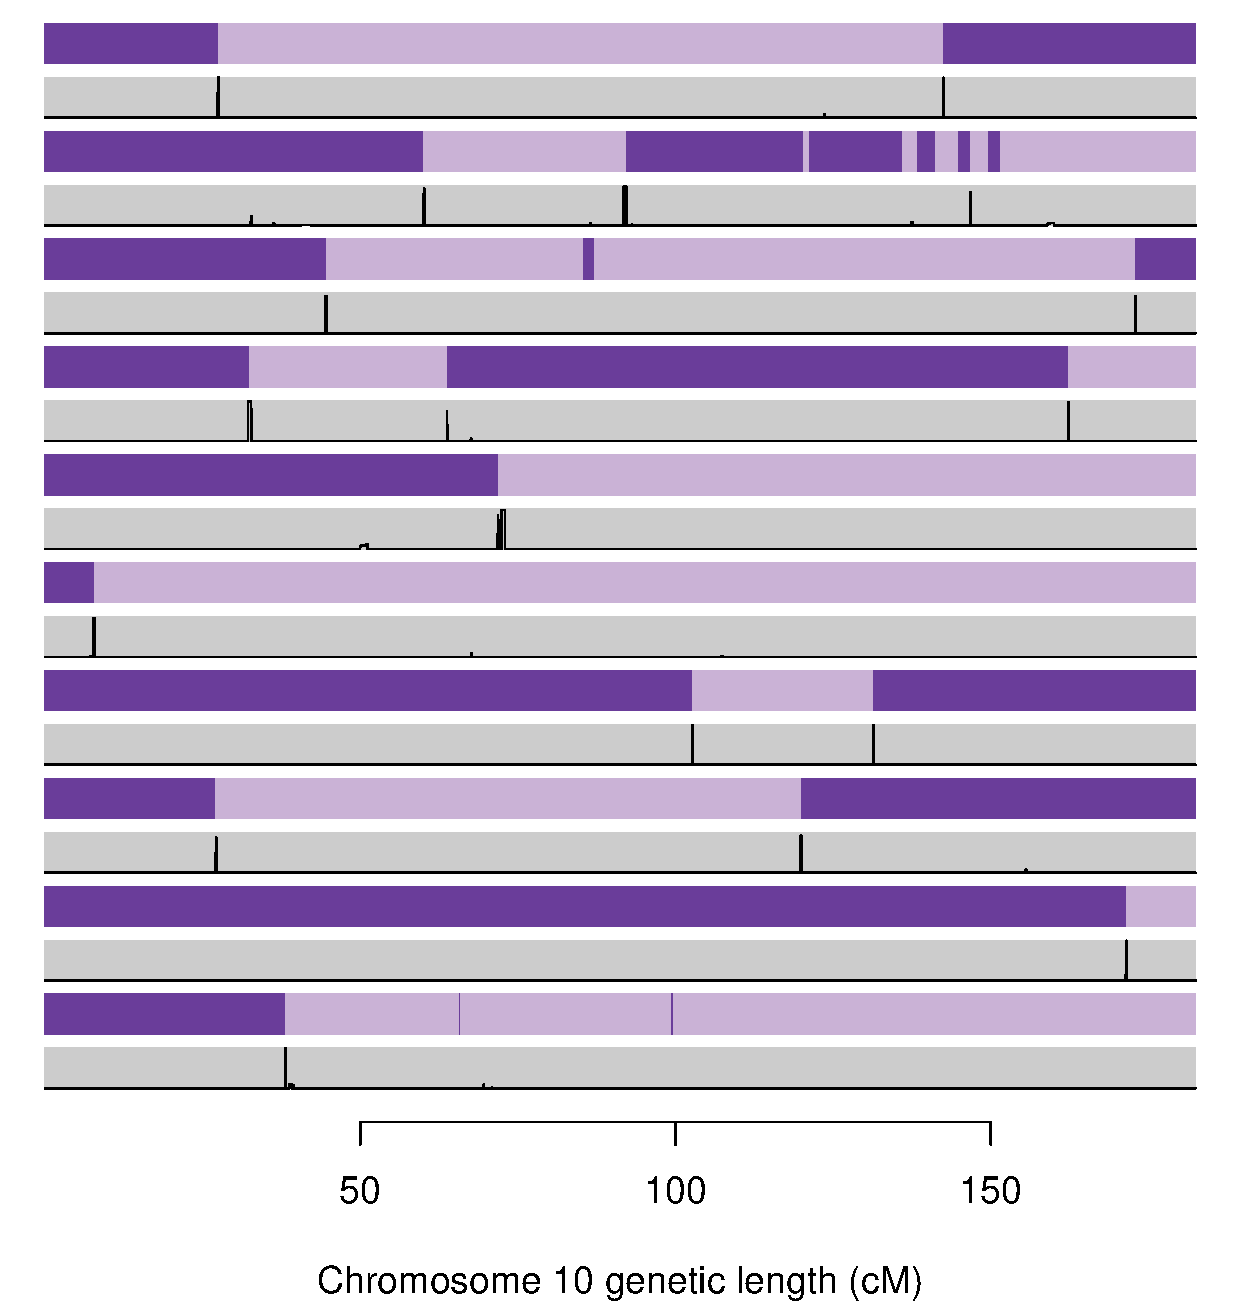
\includegraphics[width=\textwidth]{chap4figs/Fig4}
  \caption[Crossover detection (Merlin and DuoHMM) on ten real meioses]{Inferred gene flow by Merlin (purple) and our method (grey) for ten informative meioses on chromosome 10 taken from Val Borbera cohort pedigrees.  The light and dark purple represent genetic material from the grand-paternal and grand-maternal chromosomes (as inferred by Merlin's Viterbi algorithm), hence changing from light to dark implies a a recombination event.  The grey rectangles contain the posterior probability of recombination from our method.  The two methods broadly agree, although Merlin has inferred a number of implausibly small crossover events.\label{fig:shapeit-merlin}}
 \end{center} 
\end{figure}

Table~\ref{tab:pedtab2} reports the percentage of Merlin recombinations that fall within a recombination region found by our method, and the percentage of our recombination regions that contain a Merlin recombination event. Percentages are given for each cohort separately. These results show only a rough concordance between Merlin and our method, with between 41\% and 61\% of Merlin recombinations detected by SHAPEIT2 and 80\% to 89\% of SHAPEIT2's recombination events concordant with Merlin.  
\newpage
Table~\ref{tab:pedtab2} table  also shows the mean number of recombination events found by each method in maternal and paternal meioses.  For comparison, the frequently cited deCODE 2002 genetic map estimated an average of 25.9 and 42.81 autosomal recombinations per maternal and paternal meioses respectively. The average number of recombinations for Merlin was substantially inflated across most cohorts (53 to 105 for maternal and 31 to 79 for paternal events) whilst SHAPEIT2's were in a more reasonable range (25 to 29 for paternal events and 41 to 47 for maternal events). Figure~\ref{fig:merlin-shapeit-rec} plots the number of events found per meiosis by SHAPEIT2+duoHMM versus Merlin, there is obvious correlation but Merlin is typically reporting a much larger number of events than SHAPEIT2+duoHMM. 


\begin{table}
\begin{center}
\begin{tabular}{|l|rr|rr|rr|rr|}
  \hline 
  & \multicolumn{2}{c|}{Meioses}   & SHAPEIT2   & Merlin  & \multicolumn{2}{c|}{Merlin} & \multicolumn{2}{c|}{SHAPEIT2} \\
  Cohort & P & M & concordance \% & concordance \% & P & M & P & M\\

    \hline
    CARL & 24 & 47 & 80.40 & 41.28 & 63.08 & 74.57 & 25.46 & 41.81 \\ 
    FVG & 50 & 96 & 88.97 & 60.65 & 34.90 & 61.04 & 25.02 & 42.23 \\ 
%    GPC & 69 & 75 & 88.23 & 36.60 & 79.32 & 105.48 & 29.22 & 47.07 \\ 
    KOR & 4 & 11 & 80.59 & 57.16 & 39.75 & 63.64 & 28.75 & 44.82 \\ 
    ORC & 40 & 45 & 86.33 & 50.89 & 30.85 & 85.11 & 25.73 & 43.47 \\ 
    VB & 72 & 104 & 88.72 & 52.26 & 55.19 & 61.07 & 25.17 & 40.91 \\ 
    VIS & 12 & 14 & 82.81 & 58.84 & 43.75 & 52.57 & 26.83 & 41.00 \\ 
    \hline
  \end{tabular}
\end{center}

\caption[Summary of crossover events detected by DuoHMM and Merlin in real data]{Comparison of recombination detection using our  method and Merlin for all informative paternal (P) and maternal (M) meioses events in each cohort. Specificity is the proportion of recombination events flagged by our method that were also flagged by Merlin. SHAPEIT2 concordance is the percentage of SHAPEIT2 crossover events that intersected a Merlin crossover event the proceeding column is vice versa. We also provide the mean number of paternal/maternal recombination events detected for informative meioses by Merlin and SHAPEIT2. For comparison, the frequently cited deCODE 2002 genetic map estimated an average of  42.81 and 25.9 autosomal recombinations per paternal and maternal meioses respectively.  SHAPEIT2's estimates are consistently closer to the deCODE values which are considered to be of high quality.  \label{tab:pedtab2}}
\end{table}

\begin{SCfigure}
   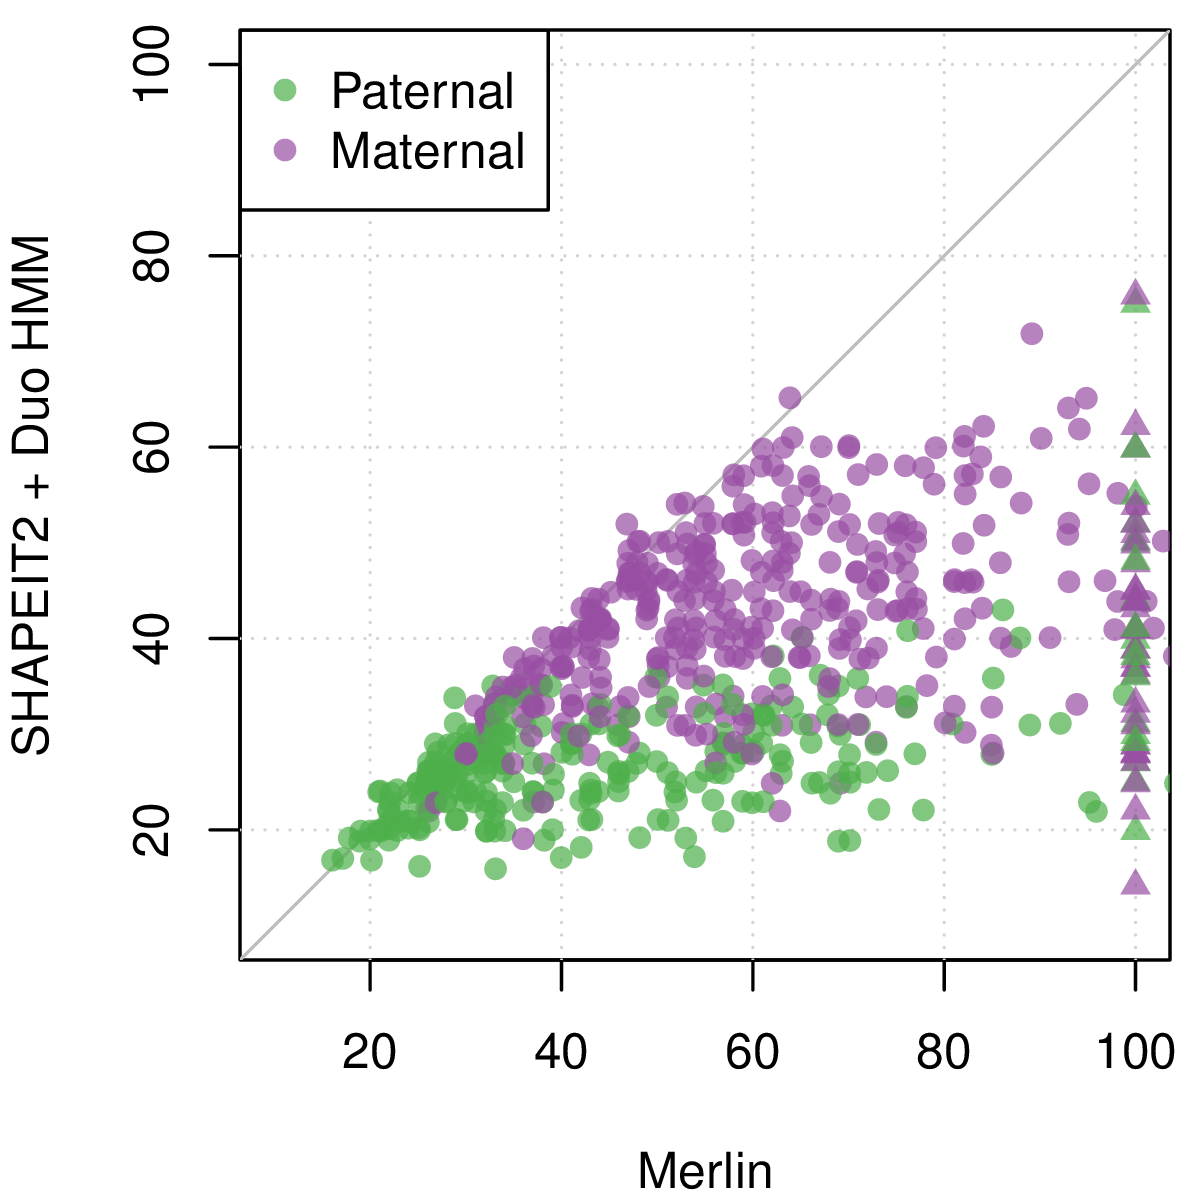
\includegraphics[width=.5\textwidth]{chap4figs/combined-merlin-vs-shapeit}    
   \centering
  \caption[Recombination rates per individual found by DuoHMM against Merlin]{Genome-wide number of recombinations found per individual for SHAPEIT versus Merlin for all informative meioses in real data sets. The number of recombinations found by SHAPEIT2 against Merlin for each of 661 meioses (all informative duos from all cohorts).  Maternal are in green and paternal purple. Triangles represent a truncated value.  While there is correlation between the two methods, Merlin more frequently finds an implausible number of recombinations.\label{fig:merlin-shapeit-rec}}
\end{SCfigure}

\begin{SCfigure}
\centering
   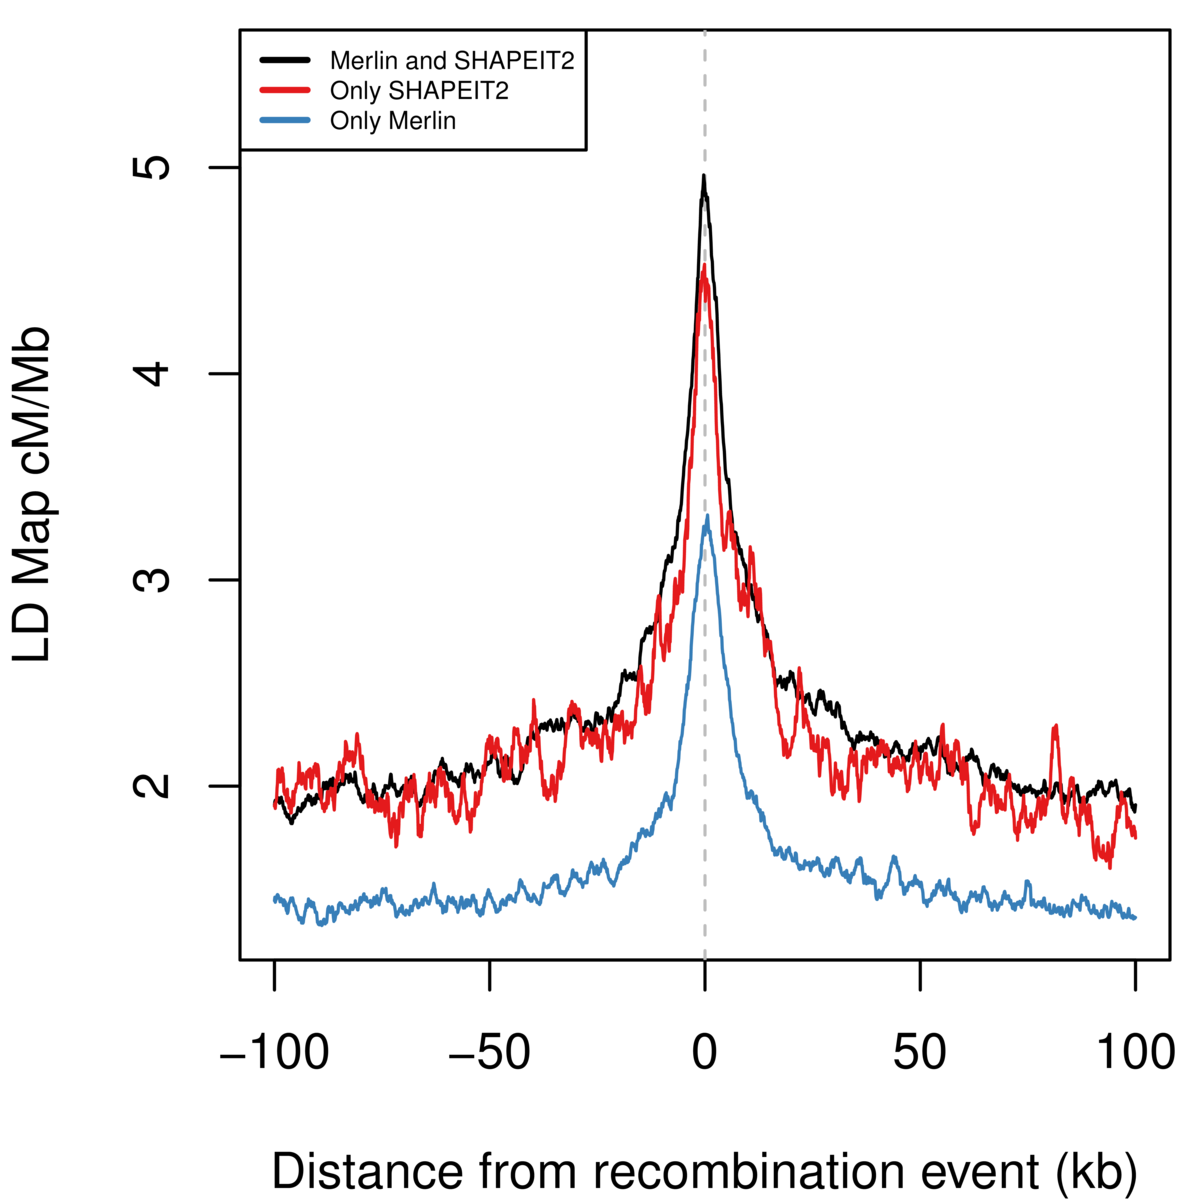
\includegraphics[width=.5\textwidth]{chap4figs/recombination_rate}
  \caption[HapMap recombination rates around detected crossover events]{Recombination rates in regions around crossover detections by each method. Average recombination rate (from the HapMap LD map) centred on the location (the average of the two flanking heterozygous positions) of 34344 crossovers found by both SHAPEIT2 and Merlin (black), 4127 crossovers found only by SHAPEIT2 (red) and 32580 crossovers found only by Merlin (blue).  Events found only by Merlin are in regions with less recombination on average than those found by by SHAPEIT2 suggesting a higher false detection rate. The Merlin map is still peaked, suggesting not all events detected were false positives.\label{fig:avg_map}}
\end{SCfigure}
\newpage
 Figure~\ref{fig:rec_summary_2} compares the distribution of the number of recombination events found by Merlin and our method to what we would expect according to the 2002 deCODE family based map. Figure~\ref{fig:rec_summary_2} (top) plots the observed against expected number of recombinations in paternal and maternal meioses for each chromosome.  The results from SHAPEIT2 are  well calibrated against the expectation, whereas the Merlin haplotypes exhibit elevated levels of recombination.  Figure~\ref{fig:rec_summary_2} (bottom) shows  QQ-plots comparing the observed and expected number of genome-wide recombinations in paternal and maternal meioses for each duo when using a Poisson distribution with rates 25.9 (paternal) and 42.81 (maternal) as our expected distribution.  SHAPEIT2 rates are well calibrated against the expectation for paternal meioses, with some over-dispersion present in maternal meioses compared to the Poisson model. 

\begin{figure}
 \begin{center} 
 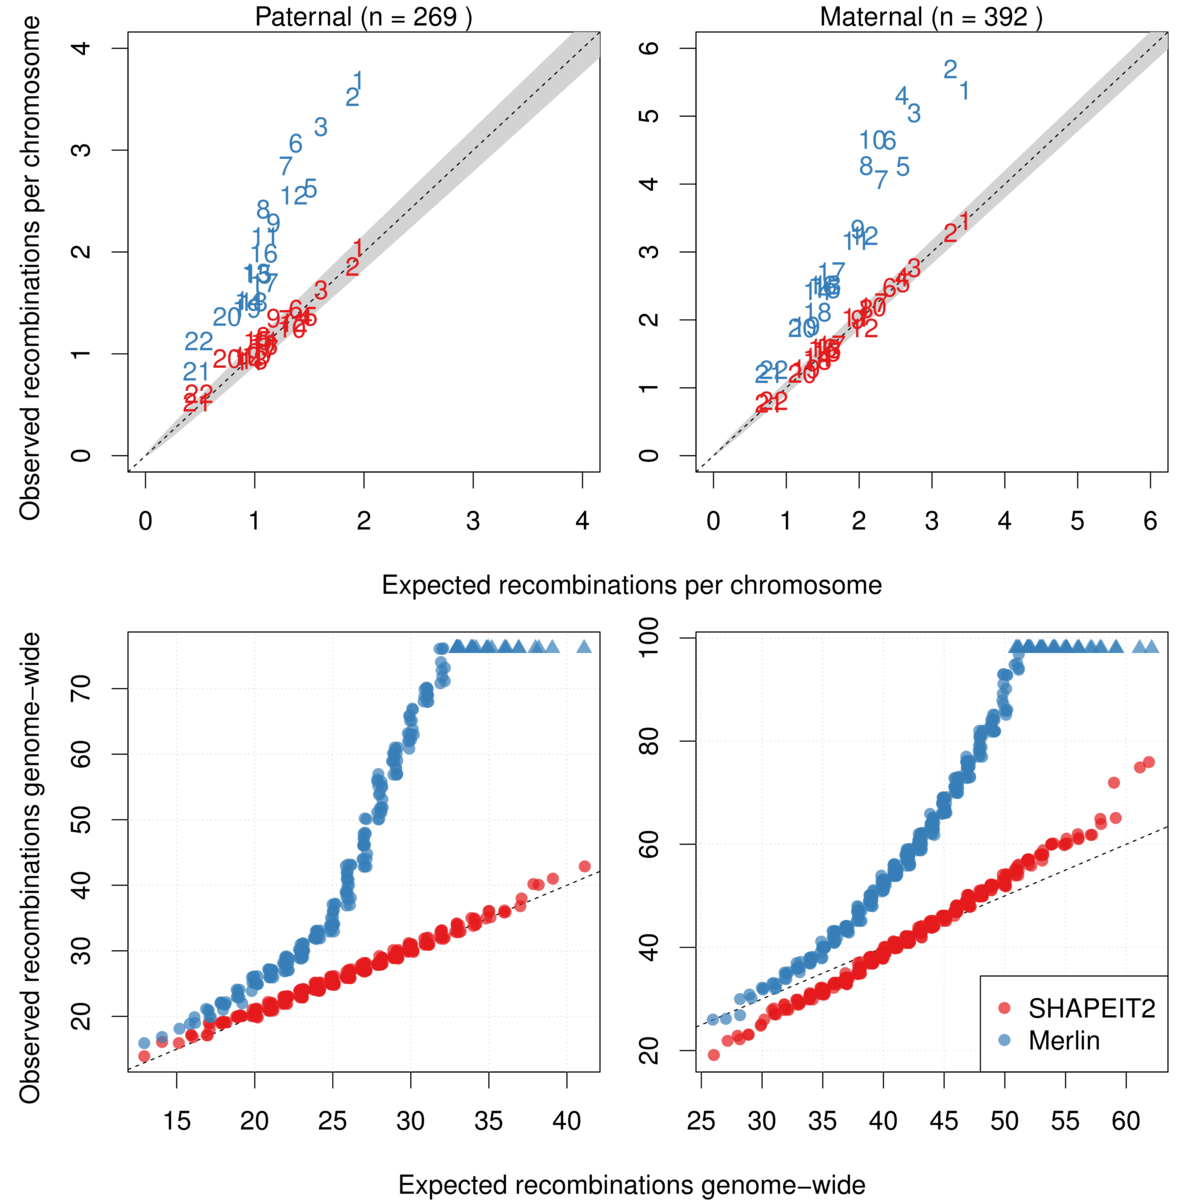
\includegraphics[width=\textwidth]{chap4figs/Fig5}
   \caption[Distributions of the number of detected crossovers for all cohorts]{Distributions of the number of detected crossovers for all cohorts. \textbf{Top:} The mean number of recombinations per meiosis (for all informative duos from all cohorts) found for each chromosome against the expected number (from the 2002 deCODE map) for paternal meioses (left) and  maternal meioses (right). Merlin's values are substantially inflated whilst SHAPEIT2's are more consistent with the well known deCODE map. \textbf{Bottom:}  Q-Q plots for the observed against expected number of recombinations estimated by each method for paternal meioses (left) and maternal meioses (right), only duos that were part of an informative pedigree were used.  For the expected distribution of recombination rates, a Poisson distribution using the genetic lengths from the 2002 deCODE Map was used (with rate parameter 42.81 and 25.9 for maternal and paternal recombinations respectively).  SHAPEIT2's rates are less inflated than those of the Merlin.\label{fig:rec_summary_2}}
 \end{center} 
\end{figure}

Figure~\ref{fig:avg_map} shows the average fine-scale recombination rate as a function of distance from the inferred recombination events inferred by both SHAPEIT2 and Merlin (black), only SHAPEIT2 (red) and only Merlin (blue).  The distribution of recombination rates around the SHAPEIT2-only crossovers is close to the distribution of crossovers found by both methods, whilst the recombination rates near Merlin events are on average lower.  It is notable that the Merlin average is still very peaked, there are several contributing factors to this.  Some of the Merlin detections will be true events that duoHMM has missed, some will be true events that duoHMM has also detected but the methods have assigned the event to a slightly different region (for example the adjacent pair of heterozygote sites) and finally some of the events will be completely spurious.  The first two cases are not false positives and will occur in regions with high recombination rates. The final case should occur uniformly across the chromosome, flattening the average map.  

These results on both simulated and real data point to elevated false discovery rates for recombination detection with Merlin, corroborating what has previously been reported in the literature~\citep{coop2008high} whereas the SHAPEIT2+duoHMM method can constrain FPR whilst still detecting a substantial proportion of true crossover events.



\clearpage
\subsubsection{Uninformative duos}
Figure~\ref{fig:roc} (left) shows ROC curves for detecting recombination events applied to our simulated uninformative meioses.  We found that recombination events could be detected with low false discovery rates, but the power of the method to detect recombination events is clearly limited by the demography of the sample.  When closely related individuals were not removed we see that 53.51\% of events could be detected with a false discovery rate  of 5\%, but when closely related individuals were filtered we could only detect 34.10\% of events with 5\% false discovery rate (posterior probability threshold of 0.7).  Importantly, the posterior probabilities of a recombination event appear roughly calibrated (Figure~\ref{fig:roc} right) so by setting a high probability threshold, researchers can be confident they are detecting true events with our method.  

\begin{figure}[h]
 \begin{center} 
  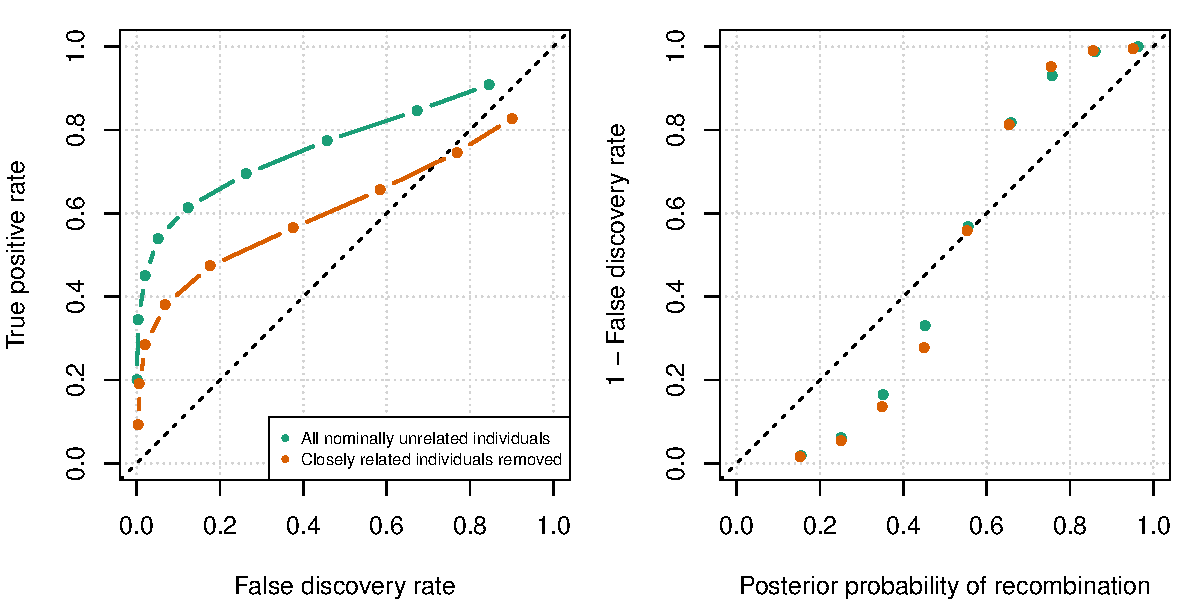
\includegraphics[width=\textwidth]{chap4figs/Fig6}
   \caption[Recombination detection accuracy in simulated uninformative duos]{ Recombination detection accuracy in uninformative duos simulated from chromosome X data in the Val Borbera cohort.  The green values are for a cohort with nominally unrelated individuals and the orange values are for a cohort that has been filtered such that no individuals are closely related ($r<0.35$)     
     \textbf{Left:} The ROC curves for recombination detection
     in uninformative duos  for our duo HMM using the SHAPEIT2 haplotypes.
     \textbf{Right:} The average number of correct detections against
     the average posterior probability.  Setting a high probability threshold ensures a very low false discovery rate.
\label{fig:roc}}
 \end{center} 
\end{figure}

\clearpage
\subsubsection{Using detected recombinations for association scans of hotspot usage} Figure~\ref{fig:hotspot} (top) shows the signal of association in the \emph{PRDM9} region for a meta analysis of all cohorts.  When only the 618 informative parents were used (top) we found a minimum P-Value of $6.25 \times 10^{-11}$ at SNP rs2162866. The addition of 466 individuals lead to a modest increase in signal ($\textrm{P-value}=3.31\times 10^{-12}$) at the same SNP. Figure~\ref{fig:hotspot} (right) plots the $-\log_{10}\textrm{P-values}$  when all individuals are used against the $-\log_{10}\textrm{P-values}$  when only informative individuals are used, demonstrating a consistent increase in signal in the region and suggests that our method is indeed detecting true recombination events.

\begin{figure}[h]
\vspace{10pt}
        \centering      
   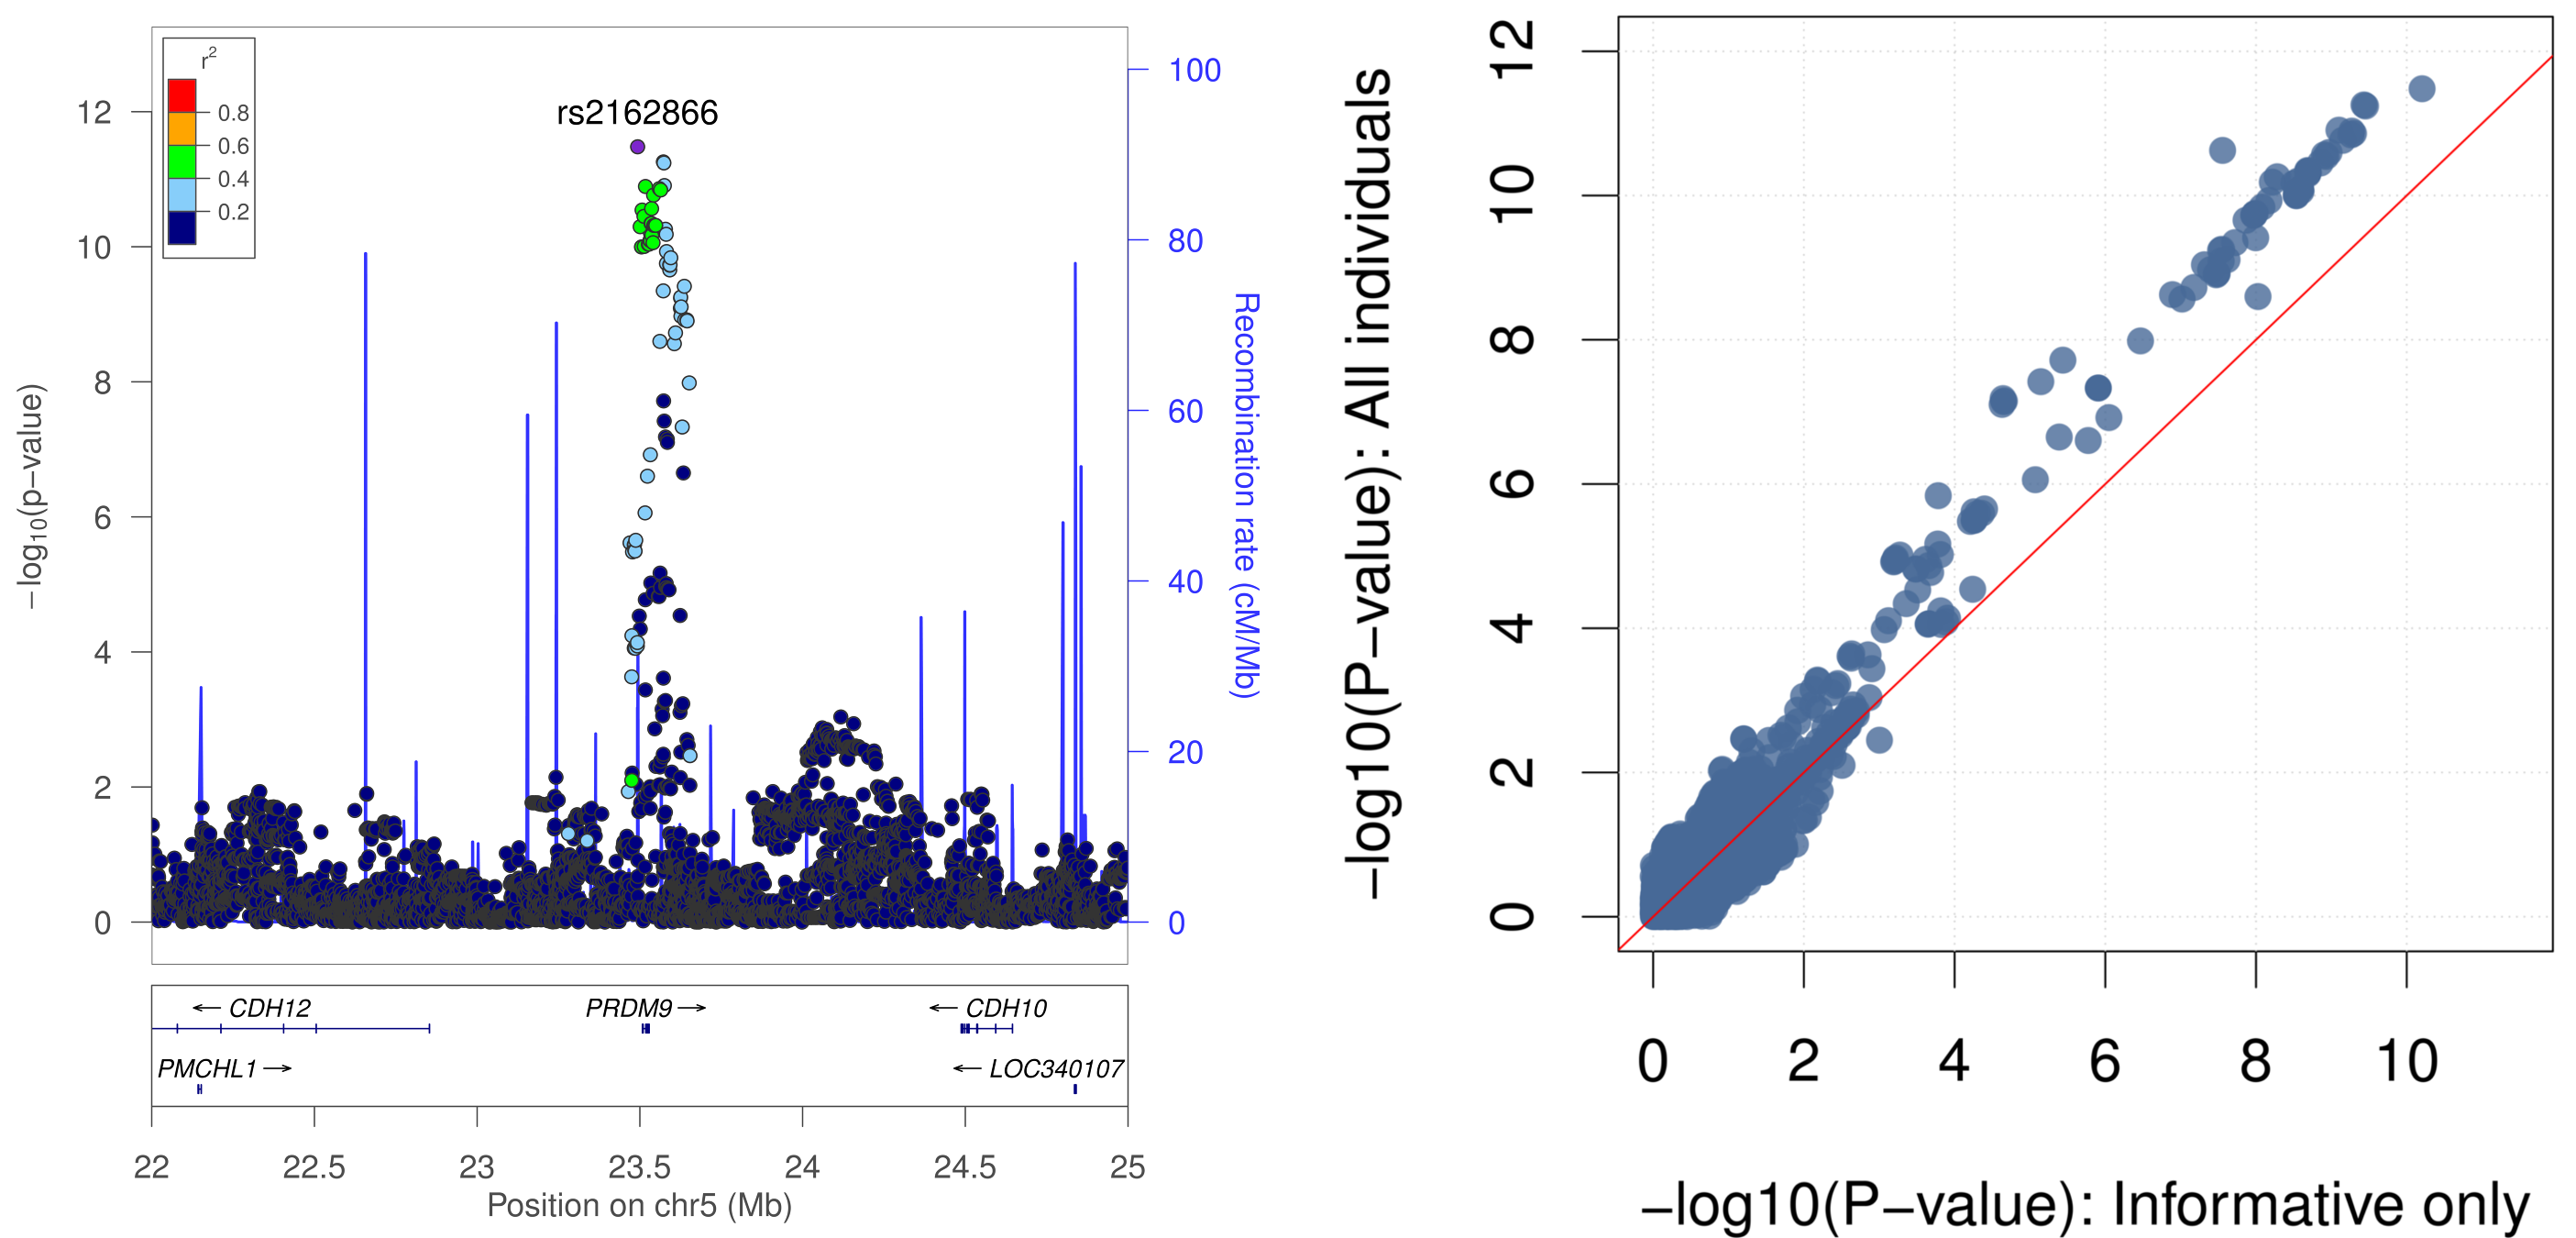
\includegraphics[width=\textwidth]{chap4figs/prdm9}
  \caption[Association testing between \emph{PRDM9} region and hotspot usage phenotype] {Association testing between \emph{PRDM9} region and hotspot usage phenotype for European cohorts. \textbf{Top:} The $-\log_{10}\textrm{P-values}$ for the European meta-analysis for association between PRDM9 variants and the `hotspot usage' phenotype.  We used 618 informative and 466 uninformative parents in this analysis. \textbf{Right:} The $-\log_{10}\textrm{P-values}$ of this analysis plotted against the  $-\log_{10}\textrm{P-values}$ when only the 618 informative parents are used.  The additional samples yield a modest increase in power. \label{fig:hotspot}}
\end{figure}

\clearpage
\subsection{Performance of error detection routine}
Throughout the pedigree experiments detailed in this chapter (both real and simulated) we have applied Merlin's error detection routine and flagged likely erroneous genotypes as missing throughout the pedigree before continuing with downstream analyses for all methods. This was to ensure all methods are analysing exactly the same data so that comparisons are fair.  In practice, converting genotype data to and from Merlin's file formats  is an arduous process that many practitioners will find inconvenient.  Hence we evaluated whether our duoHMM error detection routine would be sufficient.

We ran SHAPEIT2 on the realistic extended pedigree data described in section~\ref{chap4:pedsim1} without removing genotypes flagged as erroneous by Merlin. Mendelian inconsistent genotypes were still removed throughout a pedigree as there is no uncertainty about where an error has occurred (100\% TPR and 0\% FPR).  Since we know where true genotyping errors occurred in this data we can evaluate the TPR and FPR of the duoHMM and Merlin. Figure~\ref{generr-roc} plots the ROC curve for both methods.  Both methods can control false positives well but SHAPEIT2+duoHMM have substantially higher rate of detection.  At a 1\% FPR SHAPEIT2+duoHMM detect 71.1\% of errors whilst Merlin can only find 31.3\% of errors.  %Merlin was originally developed with far sparser data sets in mind. The original paper also found that power is decreased substantially when there are ungenotyped parents present (which is the case in some of our pedigrees) so this may explain the very large discrepancy.


\begin{SCfigure}[1][h]
\centering
   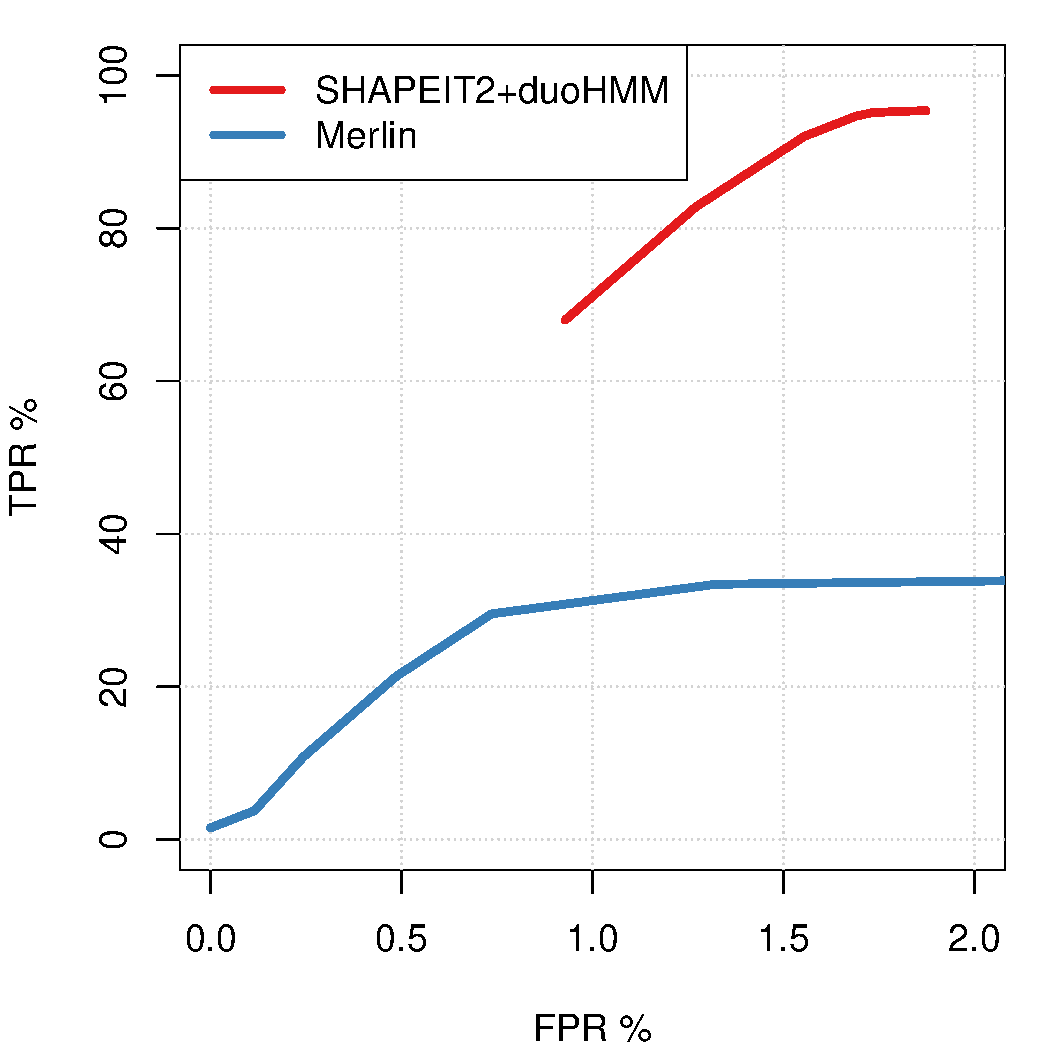
\includegraphics[width=.45\textwidth]{chap4figs/error_detection}%\vspace{-20pt}
\caption[ROC curve for the DuoHMM and Merlin genotyping error detection]{ROC curve for the duoHMM's and Merlin's genotyping error detection routines applied to the simulated extended where founders were created by merging male X chromosome data.  Both methods can control FPR well but the duoHMM has substantially greater power than Merlin.\label{generr-roc}}
\end{SCfigure}

\clearpage
\section{Discussion}

Long range phasing has been a topic of interest since its inception by \cite{kong2008detection} and has great potential for the analysis of genomic data, particularly as cohort sizes increase and hence more IBD sharing becomes present within individuals.  Whilst the deCODE project has generated some excellent results, they have the advantage of an extremely powerful data set containing substantial amounts of IBD sharing which allows a rule based approach to long range phasing that yields very accurate haplotypes.  This is not a luxury available to many research groups. We demonstrate that SHAPEIT2 implicitly performs this very accurate long range phasing when possible whilst still leveraging LD when it is not.

Using seven cohorts from isolated and non-isolated populations, all containing explicitly related individuals, we have carried out a comprehensive evaluation of approaches for haplotype estimation in the presence of IBD sharing. We compared approaches that are specifically focused on estimation of haplotypes in isolated samples (SLRP) and others (SHAPEIT2, Beagle and HAPI-UR) that were designed predominantly for cohorts of nominally unrelated individuals. Our experiments show convincing evidence that the SHAPEIT2 method provides high quality haplotypes that are more accurate than those estimated by SLRP, whereas Beagle and HAPI-UR produce results that are worse than SLRP. We find that the SE rates of SHAPEIT2 are a fraction of a percent in all cohorts, whereas the approaches BEAGLE and HAPI-UR produce SEs that are an order of magnitude larger. 

Although pedigree analysis software such as Merlin is very mature and highly regarded, its utility for phasing large cohorts containing mixtures of pedigrees and unrelateds is limited for several reasons. In particular, the inability to leverage wider cohort information to resolve sites that are heterozygous throughout a particular pedigree  prevents such software being conveniently used as part of pre-phasing and imputation pipelines.  Such pipelines are of special of interest to  groups who are sequencing pedigree founders as a cost effective way to infer novel variants throughout their cohorts via imputation.  Hence there is a need for  software that can fully leverage the relatedness within pedigrees for accurate phase whilst overcoming the limitations of traditional pedigree analysis software.  We have shown via analysis of real and simulated that SHAPEIT2 fills this niche.

Even though the SHAPEIT2 haplotypes inferred by ignoring all explicit pedigree information are very accurate we have also developed a method of incorporating available pedigree information to further increase accuracy. To do this we have developed a novel HMM that infers the inheritance pattern in parent-child duos. Having applied this approach to the SHAPEIT2 haplotypes we can detected genotyping errors, correct SEs within child haplotypes and sometimes in the parental haplotypes when enough pedigree information is available. When we apply this correction procedure to the haplotypes inferred by Beagle and HAPI-UR we observed substantial improvements in SE rate.

We have found that the resulting haplotypes from our method are so accurate that we can infer recombination events in parent-child duos. We use the output of our duoHMM to estimate the probability that a recombination event occurs between each pair of heterozygous markers in the respective parents. When applied to all seven cohorts across the whole genome we find that the number of recombination events inferred by our method shows close agreement with the genetic map length of each chromosome. We also find that the observed number of recombination events per individual closely matches what we expect to observe based on genetic map estimates. These results are also much better than those produced from Merlin, which shows elevated rates of recombination events across all chromosomes. Simulation results corroborate that our method has good power and well controlled false discovery rates when detecting crossovers.

An additional benefit of our method is that we can attempt to infer recombination events in trios and duos. Methods that explicitly phase trios and duos using the pedigree information cannot infer recombination events since they infer only the transmitted haplotypes of the parents. We evaluated this approach via simulation and found  that we have have $\sim$53\% power to detect events at a 5\% false discovery rate when the duo is phased in an isolated cohort that may contain close relatives. When close relatives are removed we have  $\sim$34\% power to detect events at a 5\% false discovery rate. Cohorts that contain explicit trios and duos could be phased using methods that explicitly use this information if desired although the ability to infer recombination events would be lost and parents would be estimated as a pair of transmitted and untransmitted haplotypes. 

Using our method we are able to demonstrate that the recombination events that we infer from otherwise uninformative duos and trios can add power to association scans for recombination phenotypes. Specifically, at the established \emph{PRDM9} locus we are able to show that including these extra recombination events increases the signal of association for a hot spot usage phenotype.

Precisely determining why these large differences in performance between the methods exist is difficult. We suspect that the reason resides in the fact that within the SHAPEIT2 method the haplotypes of each individual are explicitly modelled as a mosaic of the underlying haplotypes of other individuals~\citep{li2003model}. In other words the underlying haplotype sharing between two individuals can be explicitly captured by allowing each individual to `copy' the haplotypes of another individual over a long stretch of sequence. Beagle and HAPI-UR take a different approach by collapsing the haplotype information of the conditioning haplotypes into compact graphs. Each individual's haplotypes are then updated within the method conditional upon this graph. Thus no direct comparison between pairs of individuals is made and the information regarding long stretches of shared sequence between individuals is lost.  Hence whilst these collapsing approaches allow fast computation, they appear to have a substantial cost in terms of accuracy when there is large IBD sharing within a cohort.

SHAPEIT2 has already been shown to be the most accurate phasing method for cohorts of unrelated individuals but performance in cohorts with different demographies had not yet been evaluated.  The results in this chapter demonstrated SHAPEIT2's surprising ability to leverage the full range of relatedness for accurate haplotype inference.  The duoHMM we introduced builds on SHAPEIT2's accuracy even further enabling some of the analyses available in more typical pedigree phasing routines such as recombination detection and the detection of subtle genotyping error as well as slightly improving haplotype accuracy.  These results should have a unifying effect on the field meaning researchers need not worry about running multiple pieces of software for phasing cohorts with eclectic demographies.




\chapter{Phasing very large samples}

SHAPEIT2 was initially published with the goal of phasing unrelated samples of individuals, and was shown to be the most accurate method for this task in its original paper. In the previous chapter we demonstrated that SHAPEIT2 is in fact the most accurate method over a surprisingly large range of demographic scenarios.  Whilst computationally tractable, SHAPEIT2 is not the fastest algorithm available.  On the samples analysed in the previous chapter, both HAPI-UR and Beagle were substantially faster.  Running times on chromosome 10 for each cohort are shown in figure~\ref{fig:timing-summary}.  We argue that for these sample sizes a factor of $\approx5$ in computation time is not a large sacrifice to make for the accuracy gains of SHAPEIT2.  Additionally SHAPEIT2 has a very convenient multi-threading functionality which means end-users can exploit multi-core systems with ease, hence the computational cost is largely mitigated for these ranges of $N$.

However, the age of $N>~$100,000 is upon us. For example the UK Biobank intends to genotype 500,000 individuals on Affymetrix Axiom microarrays\footnote{\url{http://www.ukbiobank.ac.uk/about-biobank-uk/}} and 100,000 individuals were recently assayed in Kaiser Permanente's Research Program on Genes, Environment and Health\footnote{{\url{http://www.rpgeh.kaiser.org/}}}. Phasing and imputation will be necessary to fully exploit such data sets and hence computationally tractable software for these tasks is needed.

\begin{SCfigure}
  \centering
  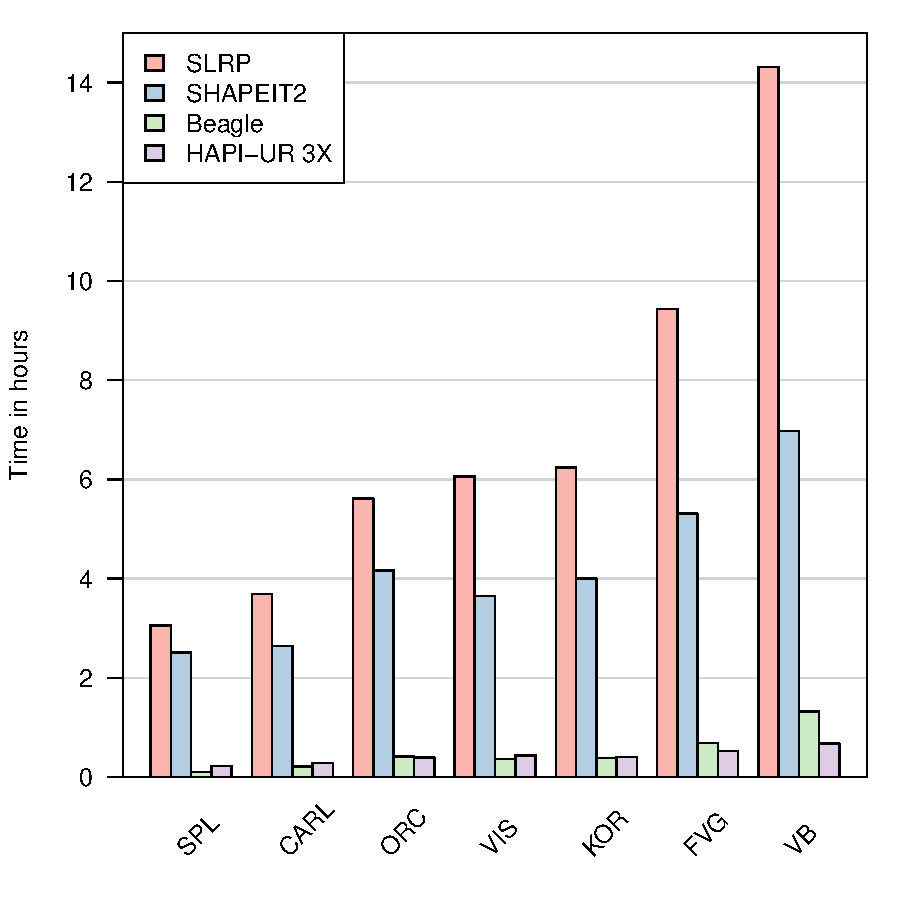
\includegraphics[width=.5\textwidth]{chap4figs/timingsummary}    
  \caption[Summary of phasing computation for isolates cohorts]{Computation time in hours for phasing chromosome 10 for each of the full cohorts described in Chapter 4.  All jobs were run on an Intel Xeon CPU E5-2690 (2.90GHz) CPU with 256GB of RAM.  Whilst no parallelism was employed here, options exists for exploiting multiple processors with varying degrees of difficulty for each piece of software.  \label{fig:timing-summary}}
%SHAPEIT2 and SLRP have the ability to run on $N$ threads resulting in an approximately $N \times$ reduction in computation time.  HAPI-UR  can be run as three simultaneous processes rather than sequentially.  Most simply, the genome can be partitioned into chunks which are phased separately with the results being ligated.
\end{SCfigure}
\newpage
In this chapter we concern ourselves with the scalability of different algorithms.  For $N=1,000$ all algorithms mentioned in the previous chapter will run within one day on a modern server with multiple CPUs, but when $N>>10,000$ the computational costs of phasing become a serious concern.  None of the techniques described in this thesis scale linearly with sample size, so na\"{\i}vely extrapolating from figure~\ref{fig:timing-summary} would be foolish.  SHAPEIT2's distance calculations incur a quadratic complexity term, but these are performed very rapidly with look-up tables so it was not clear when this quadratic component will begin to dominate computation. HAPI-UR and Beagle both need to build their respective haplotype graphs on each iteration which has complexity that is sub-quadratic but super-linear.  HAPI-UR's primary use-case is to phase very large samples tractably and it is currently the fastest method available as demonstrated in recent publications~\citep{williams2012phasing,delaneau2013}, although it is less accurate than SHAPEIT2.

In this chapter we evaluate the scalability and accuracy of HAPI-UR and SHAPEIT2 as sample sizes become very large.  We also introduce a further approximation to SHAPEIT2 to reduce the number distance calculations it has to perform, with the goal of making the non-HMM component of the algorithm scale linearly.  Since large data sets ($N>>10,000$) are currently not easy to obtain, we use a combination of real and simulated data for evaluation purposes.

\section{Reducing the complexity of SHAPEIT2's distance calculations}  
The current release of SHAPEIT2 selects a set of $K$ conditioning haplotypes for an individual being updated.  The set of $K$ conditioning haplotypes are denoted as  $H^{*}$ and are a subset of the  full set of haplotypes in the cohort, $H$. Computational cost and accuracy both increase with $K$, the default of $K=100$ generally gives good results. Chromosomes are divided into roughly equally size windows and  a different set of $H^{*}$ is chosen for different windows. Window size is a tuneable parameter and the default size for microarray data is 2Mb.  Conditioning haplotypes are selected for an individual being phased by taking the $K$ haplotypes in the sample with the closest Hamming distances from the individual's haplotypes from the previous iteration, say $(h^1,h^2)$. The idea being that this will yield more closely related conditioning haplotypes which are more informative of phase.

One caveat with this approach is that individuals that share a region of genome where \emph{both} haplotypes are identical-by-descent (IBD=2) are uninformative of phase and can cause the algorithm to get stuck in a poor quality solution.  Hence individuals that are  IBD=2 within a region are excluded from the set of possible conditioning haplotypes. Details of how the IBD=2 individuals are determined are described in the supplementary of \cite{delaneau2013}. 

The algorithm for selecting conditioning haplotypes is then as follows:

\vspace{10pt}
\begin{algorithm}
  \caption{SHAPEIT2 haplotype selection}
  \begin{algorithmic}[0]    
    \State Select $W\subseteq H$ such that haplotypes in $W$ are unlikely to be from IBD=2 individuals
    \ForAll{$H_j\in W$}
    \State    Calculate $D(H_j) = \textrm{min}(\textrm{\texttt{hamming}}(h^1,H_j),\textrm{\texttt{hamming}}(h^2,H_j))$
    \EndFor
    \State    Sort $W$ by ascending $D(H)$ values    
    \State \textbf{return} the first $K$ haplotypes in $W$
  \end{algorithmic}
\end{algorithm}
where $\textrm{\texttt{hamming}}(h,H)$ is the Hamming distance between the two haplotypes, that is the count of binary differences.

 If we assume that the number of haplotypes in $W$ is $M\approx2(N-1)$ then this algorithm has complexity $O(N^2L)$ which is undesirable when $N$ becomes large. However, the filtering of IBD=2 individuals suggests an obvious way of controlling complexity. If we could limit the size of $W$ to $M$ elements then the algorithm would have complexity $O(NML)$, if we could keep $M$ constant then we would have an algorithm with complexity $O(NL)$ which is our desired outcome.  Most simply, we could create $W$ by randomly sampling $M$ haplotypes, we refer to this method as SHAPEIT2-random. We evaluate such an approach as well a more sophisticated partitioning approach described next.  We refer to the set $W$ as the `candidate haplotypes'.  In all comparisons we set $M=1000$, further work will involve tuning this parameter.

\subsection{K-Means clustering to partition the data}
Given a set of haplotypes within a window, $H=\{H_1,\ldots,H_N\}$, we could assign class labels to each observation, say $C_i \in \{1, \ldots ,J\}$, such that observations with the same label are similar according to some metric. We can then assign the candidate haplotypes for each individual $i$ as $W_i = \{H_j: C_j =C_i \}$. This is a more a principled approach than choosing $W$ at random, but does require a fast clustering method.

K-Means clustering is a well known technique that minimises the within-cluster sum of squares:
$$\sum_{i=1}^N \sum_{l=1}^L (H_{il} - \mu_{C_i l})^2$$
where $\mu_C$ is the cluster mean for class $C$.  The simplest way to minimise this objective function is to iteratively assign class labels to each observation based on which cluster mean is closest and then recalculate the mean, continuing until convergence~\citep{lloyd1982least}. \cite{arthur2007k} proposed ``K-means++'' which provides an algorithm for choosing starting values that are well dispersed and tend to lead to convergence to better optima with less iterations.

We implemented K-means++ within SHAPEIT2 and applied it to all haplotypes within each window running it for 10 iterations or until convergence, 10 iterations is usually insufficient for convergence but we only require a rough partitioning.  If we want clusters of roughly size $M$ then we set the number of clusters $J=2N/M$. If we make the assumption that K-Means results in a perfectly equal partitioning then the SHAPEIT2 distance calculations will have complexity $O(NML)$. The K-Means algorithm has complexity $O(NIJ) = O(N^2I/M)$ where $I$ is the number of iterations.  Whilst this is still scaling quadratically with $N$, the divisor $M$ controls computation well for the sample sizes we investigate.  We refer to this modification as SHAPEIT2-kmeans.

A problem with this approach is that a haplotype's nearest neighbours are not guaranteed to be within the same cluster  and hence may not be identified.  This is likely to be the case  for individuals on the boundary of a cluster. Figure~\ref{chap5:kmeans} gives a toy example demonstrating this problem. 
\begin{SCfigure}[1][h]
  \centering
  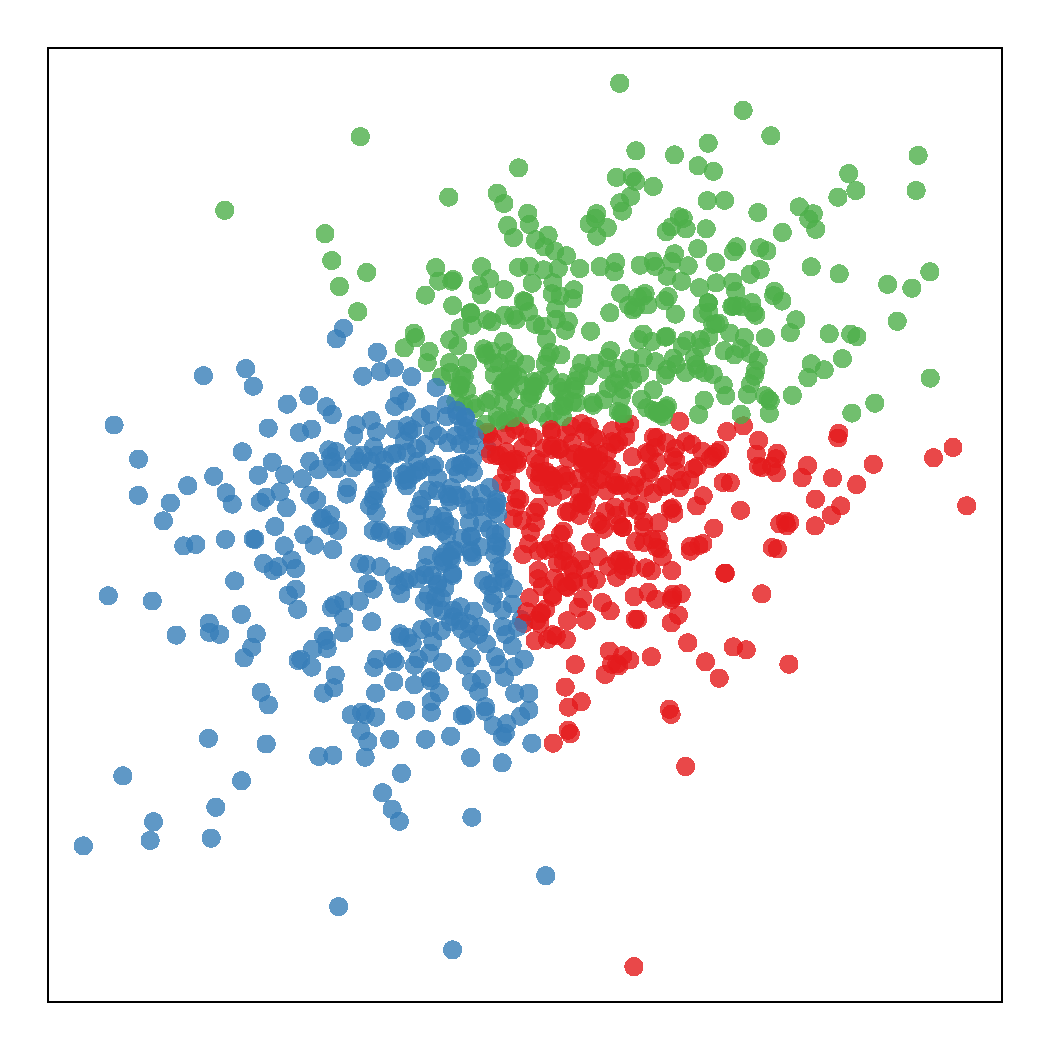
\includegraphics[width=.45\textwidth]{chap5figs/kmeans-example}
  \caption[K-Means toy example]{A toy example for K-Means on some simulated bivariate data with three clusters coloured red, green and blue.  Whilst  an observation's nearest neighbours are usually within the same cluster, points on the boundary will have nearest neighbours in a different cluster.  If we only search for nearest neighbours within the same cluster, the solution will be sub-optimal. This data is simulated on from a bivariate normal distribution which is obviously different to the haplotype data we work with, but the same principal applies.\label{chap5:kmeans}}
\end{SCfigure}

%% \subsection{Partitioning on the first principal component}
%% Principal Component Analysis (PCA) is a popular method for dimension reduction and has proved to be an extremely powerful took in genetics for quantifying broad scale relatedness between individuals using genotype data~\citep{patterson2006population,novembre2008genes,mcvean2009genealogical}.  The engine underlying PCA is the singular value decomposition (SVD) of a design matrix $X$:
%% $$\textbf{X} = \textbf{U} \textbf{D} \textbf{V}^T $$
%% here $X$ is our haplotype data with $2N$ rows and $L$ columns.  The columns of $\textbf{U} \textbf{D}$ are the principal components (PC1,PC2,...,PC$L$) of $\textbf{X}$ where the PC1 is the linear combination of genotypes with the maximum variances, PC2 is orthogonal to PC1 and has the maximum remaining variance and so forth. 

%% The SVD has complexity $O(N^2L)$ when $N>L$ (which is likely the case here), but if we have the matrix $\textbf{V}$ we can rotate $\textbf{X}$ accordingly to find the PCs.  We simply sub-sample one thousand rows of $\textbf{X}$ to calculate an approximate  $\textbf{V}$ and then rotate the full  $\textbf{X}$, finding approximate principal components constraining the SVD computation to $O(L)$. Let $\textrm{PC1}_i$ be the first principal component for haplotype $H_i$. We then choose $W_j = \{H_j : |\textrm{PC1}_i-\textrm{PC1}_j| < q_{M/2}\}$ where $q_{M}$ is the $M/(2N)$th quantile of all differences from $\textrm{PC1}_i$. That is, we find the $M$ closest values on the first principal component, these can be found with $O(M)$ complexity by storing the PC1s has a sorted list and using a binary search~\citep{skiena1998algorithm}.

%% Reducing a haplotype with hundreds of SNPs to one dimension is likely to result in a substantial loss of information so this approach is very approximate.  However the described algorithm is very fast and may prove superior to the randomised approach.

\section{Data}
\subsection{Real data}
We merged all the cases and controls from the Wellcome Trust Case Control Consortium 1~\citep{consortium2007} (WTCCC1) along with the 60 European individuals taken from the parents of 90 mother-father-child trios available from the HapMap cohorts~\citep{hapmap2}.  The parents from the trios provide us with true underlying haplotypes for individuals of similar ethnicity to those individuals in the WTCCC1 cohort.  The WTCCC1 individuals were assayed on the Affymetrix 500K genotype microarray and the HapMap individual's SNPs were filtered to match the markers on this chip.  This provides us with a sample of $N=16239$ with 60 validation individuals. We analysed 10Mb of data from chromosome 10 in these experiments (60Mb-70Mb).

\subsection{Simulated data}
We simulated genetic variants across 10Mb of DNA for 100,000 haplotypes, to create 50,000 diploid individuals. Simulations were performed using the Markovian Coalescent Simulator (MaCS) software~\citep{chen2009fast} which allows approximate simulation from the coalescent for genomic sequences up to the length of whole chromosomes with arbitrary demographic histories.  We used the demographic model specified by \cite{schaffner2005calibrating} whom calibrated the model to empirical measures of linkage-disequilibrium and the variant frequency spectrum observed in real data.  The combined genetic map from the HapMap project~\citep{hapmap2} for chromosome 1 (63Mb - 73Mb) was supplied to MaCS for simulations.  Finally we sampled variants from this simulated data in a stratified manner giving similar physical spacing between SNPs and  allele frequency spectrum to the Affymetrix 500K chip that was used on the WTCCC1 cohort described previously.  Genotyping error was introduced in the same way as described in the chapter 4 simulation experiments.

\section{Results}
We randomly sampled subsets of differing size on both the real and simulated data to evaluate how the accuracy and computation scales with sample size for each method.

\subsection{Profiling}
We first profiled the computation of the standard implementation of SHAPEIT2 on our simulated data.  Figure~\ref{chap5:s2-profile} shows what proportion of time SHAPEIT2 spends on each of its computational components as $N$ increases.  For small sample sizes the HMM component of the model completely dominates computation.  Once sample sizes increase past 10,000 the distance calculations begin to account for a substantial amount of the computation time.  For N=50,000 we estimate SHAPEIT2 would take 377.7 days to phase the whole genome (although this task would be easily parallelised), 83.6\% of this computation time would involve distance calculations.  
\begin{SCfigure}[1][h]
  \centering
  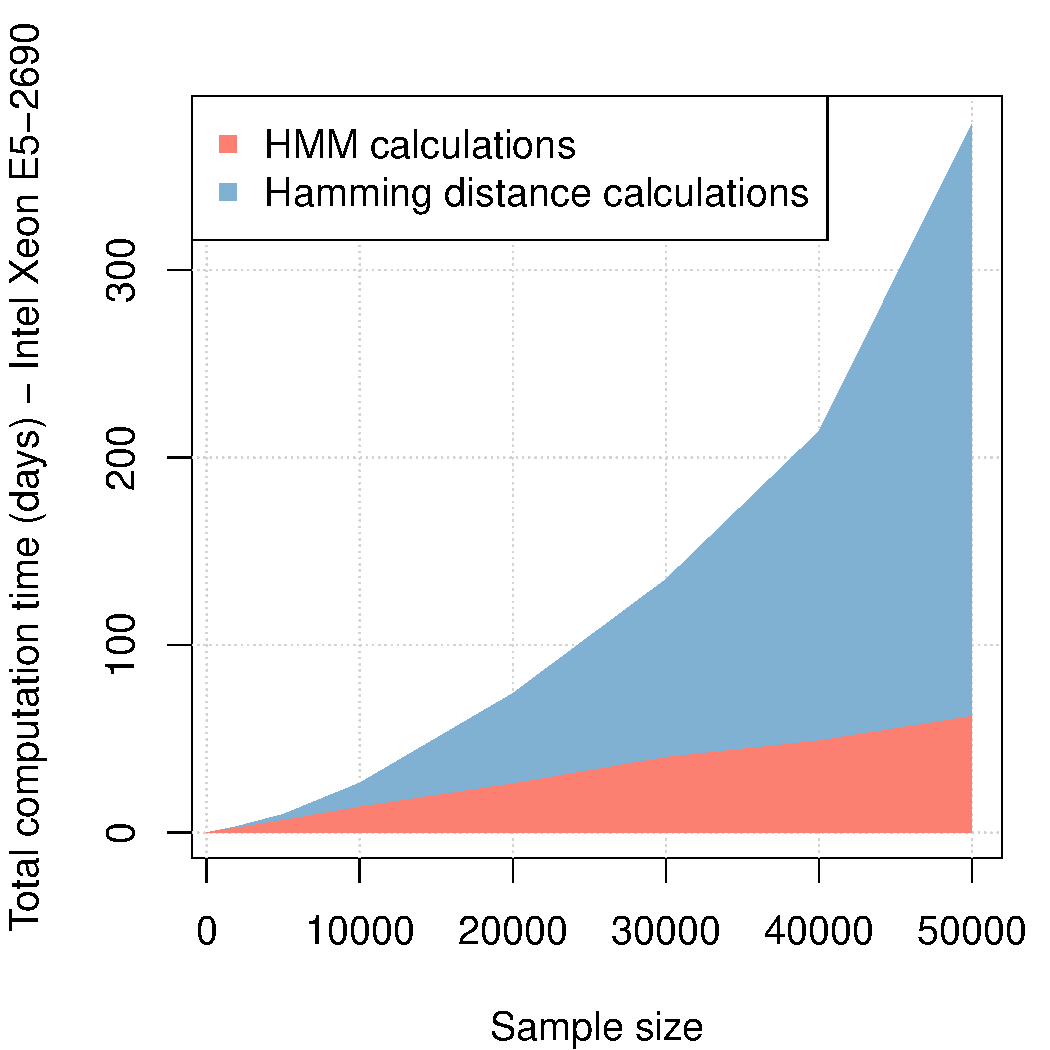
\includegraphics[width=.5\textwidth]{chap5figs/shapeit2_profiling}
  \caption[SHAPEIT computation profiling]{Profiling of the standard version SHAPEIT2's computational load on our simulated data set for increasing values of $N$. Computation time is in days (extrapolated from computations on a 10Mb region).  The blue area is the time spent on Hamming distance calculations. The light red area is the time spent on all other computations. The height of the curve is total computation time. When $N>10000$ the Hamming distance calculations rapidly begin to dominate computation. \label{chap5:s2-profile}}
\end{SCfigure}

\subsection{Performance on real data}
Figure~\ref{chap5:switch} (top) plots the switch error rate (left) and computation time in days (right) for varying sample sizes on the HapMap+WTCCC1 data. Switch error rates for N=1,000 were  2.1\%, 2.0\%, 2.15\% and 2.9\% for SHAPEIT2, SHAPEIT2-Random, SHAPEIT2-kmeans and HAPI-UR respectively which is in line with previously published results. It is interesting the random approach does marginally better here but this could just be due to the fact SHAPEIT2 is using stochastic algorithm to estimate haplotypes. Switch error for SHAPEIT2, SHAPEIT2-kmeans and HAPI-UR improve substantially as sample size increases with switch error rates of 1.28\%, 1.42\% and 1.66\% for the largest sample size of N=16,239.   SHAPEIT2-random has an error rate of 1.84\% at this sample size and appears to be beginning to plateau. SHAPEIT2-kmeans has consistently $\approx$ $0.1\%$ higher switch error than SHAPEIT2 but is still consistently more accurate than HAPI-UR.   For N=16,239, SHAPEIT2-kmeans and HAPI-UR are about 1.5 and 1.6 times faster than SHAPEIT2.  SHAPEIT2-kmeans and SHAPEIT2-random appear to be scaling linearly across this range of $N$ whilst HAPI-UR and SHAPEIT2 show greater than linear scaling.

\subsection{Performance on simulated data}
The accuracy on the simulated data is somewhat higher than what we observe on the real data sets.  At N=1,000 SHAPEIT2, SHAPEIT2-random, SHAPEIT2-kmeans and HAPI-UR  have switch error rates of 3.66\%, 3.77\%, 3.62\% and 8.79\% respectively, decreasing to  0.47\%,  3.25\%, 0.629\%  and  0.85\% for N=50,0000. The random selection method sees little improvement in accuracy after N=10,000 in this data.  SHAPEIT2 remains the most accurate method across the range of sample sizes, followed by SHAPEIT2-kmeans and then HAPI-UR.

The more interesting results are the computation times.  SHAPEIT2-kmeans scales linearly across this range of $N$ whilst the super-linear scaling of HAPI-UR  means it is slightly slower than SHAPEIT2-kmeans at N=50,000.  SHAPEIT2-kmeans is 4.57 times faster than SHAPEIT2 and 1.08 times faster than HAPI-UR  at N=50,000.  The K-means approach is also faster than SHAPEIT2-random despite having greater theoretical complexity.  This is because we put considerable effort into optimising the K-means clustering routine whilst the random generation of candidate haplotypes was implemented with a simplistic rejection sampling scheme. 

\begin{figure}
\centering
\textbf{WTCCC1 + HapMap Data}\\
   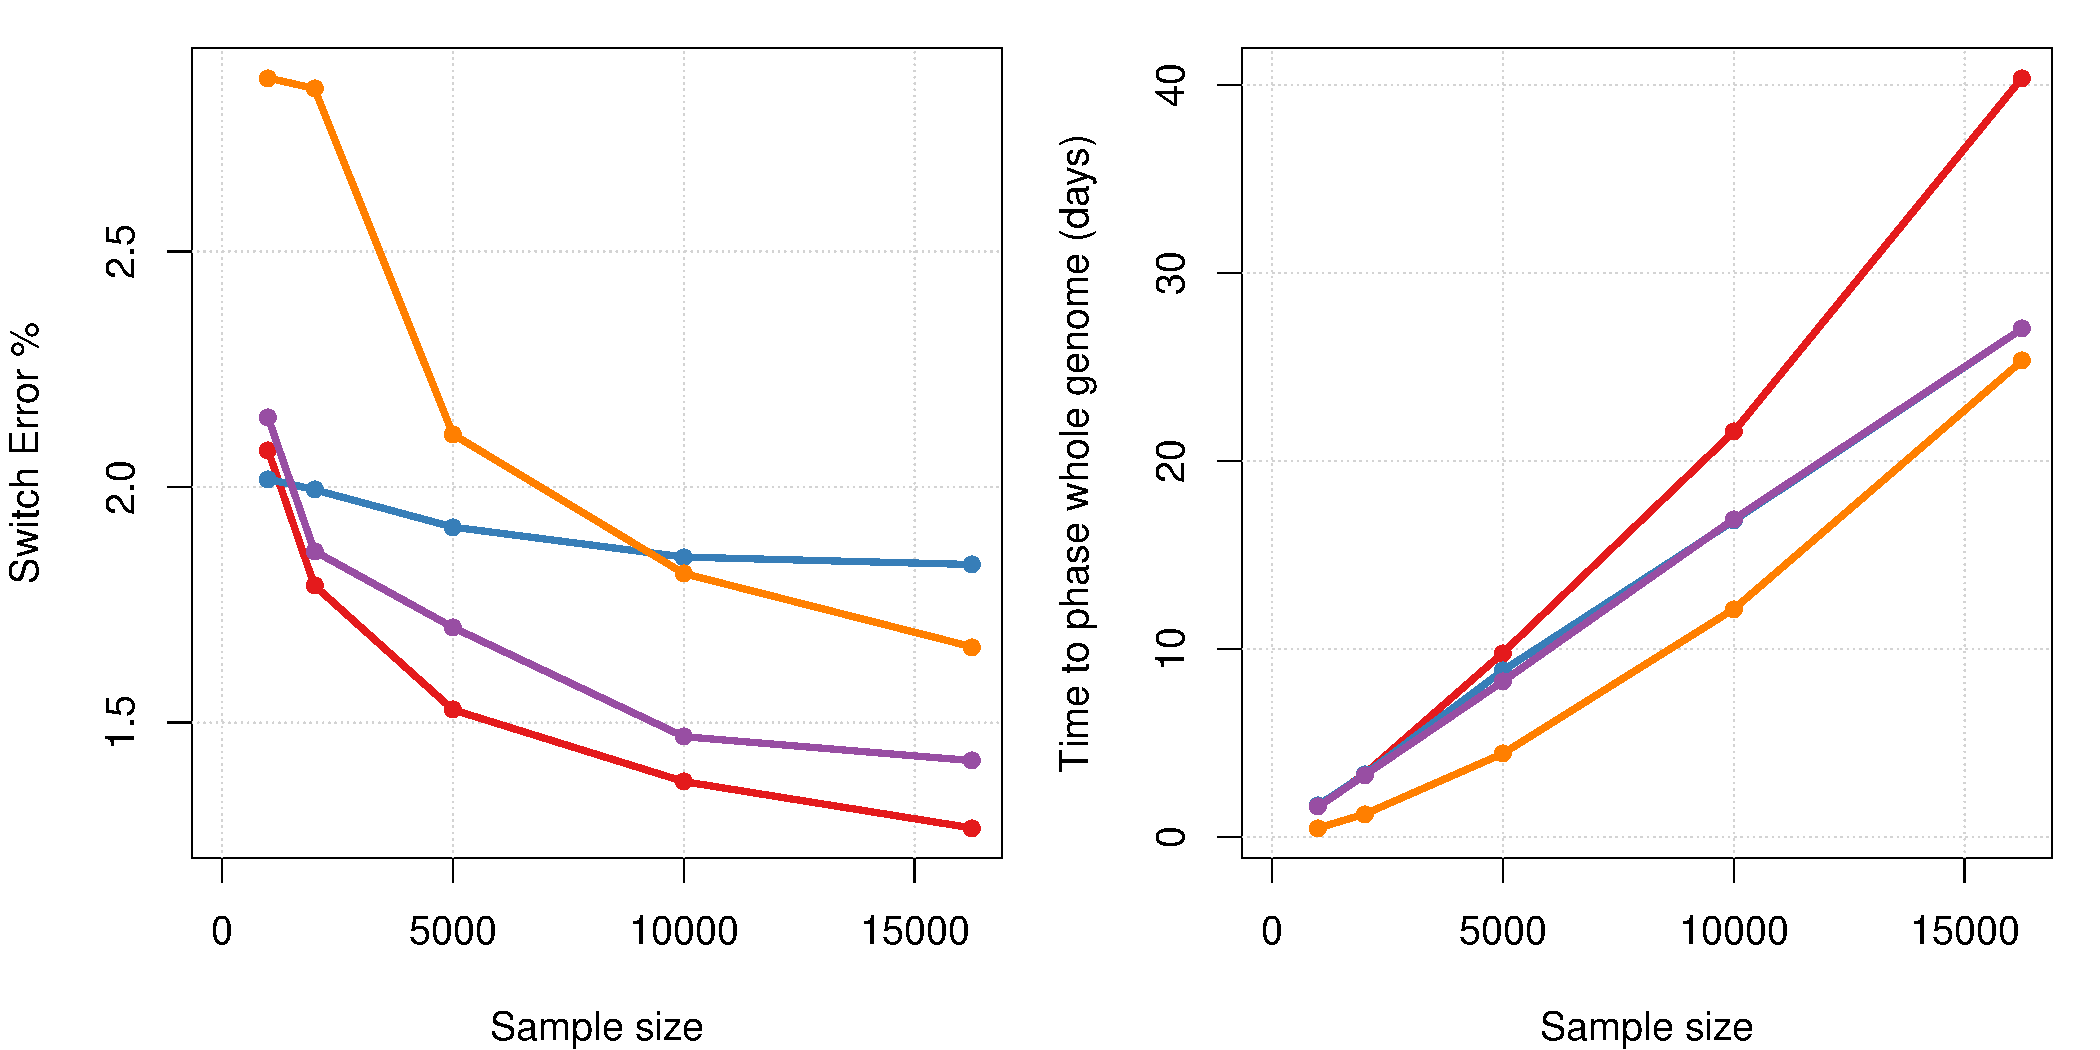
\includegraphics[width=\textwidth]{chap5figs/wtccc}\\%\vspace{-20pt}\\
\vspace{20pt}
\textbf{Simulated data}\\
   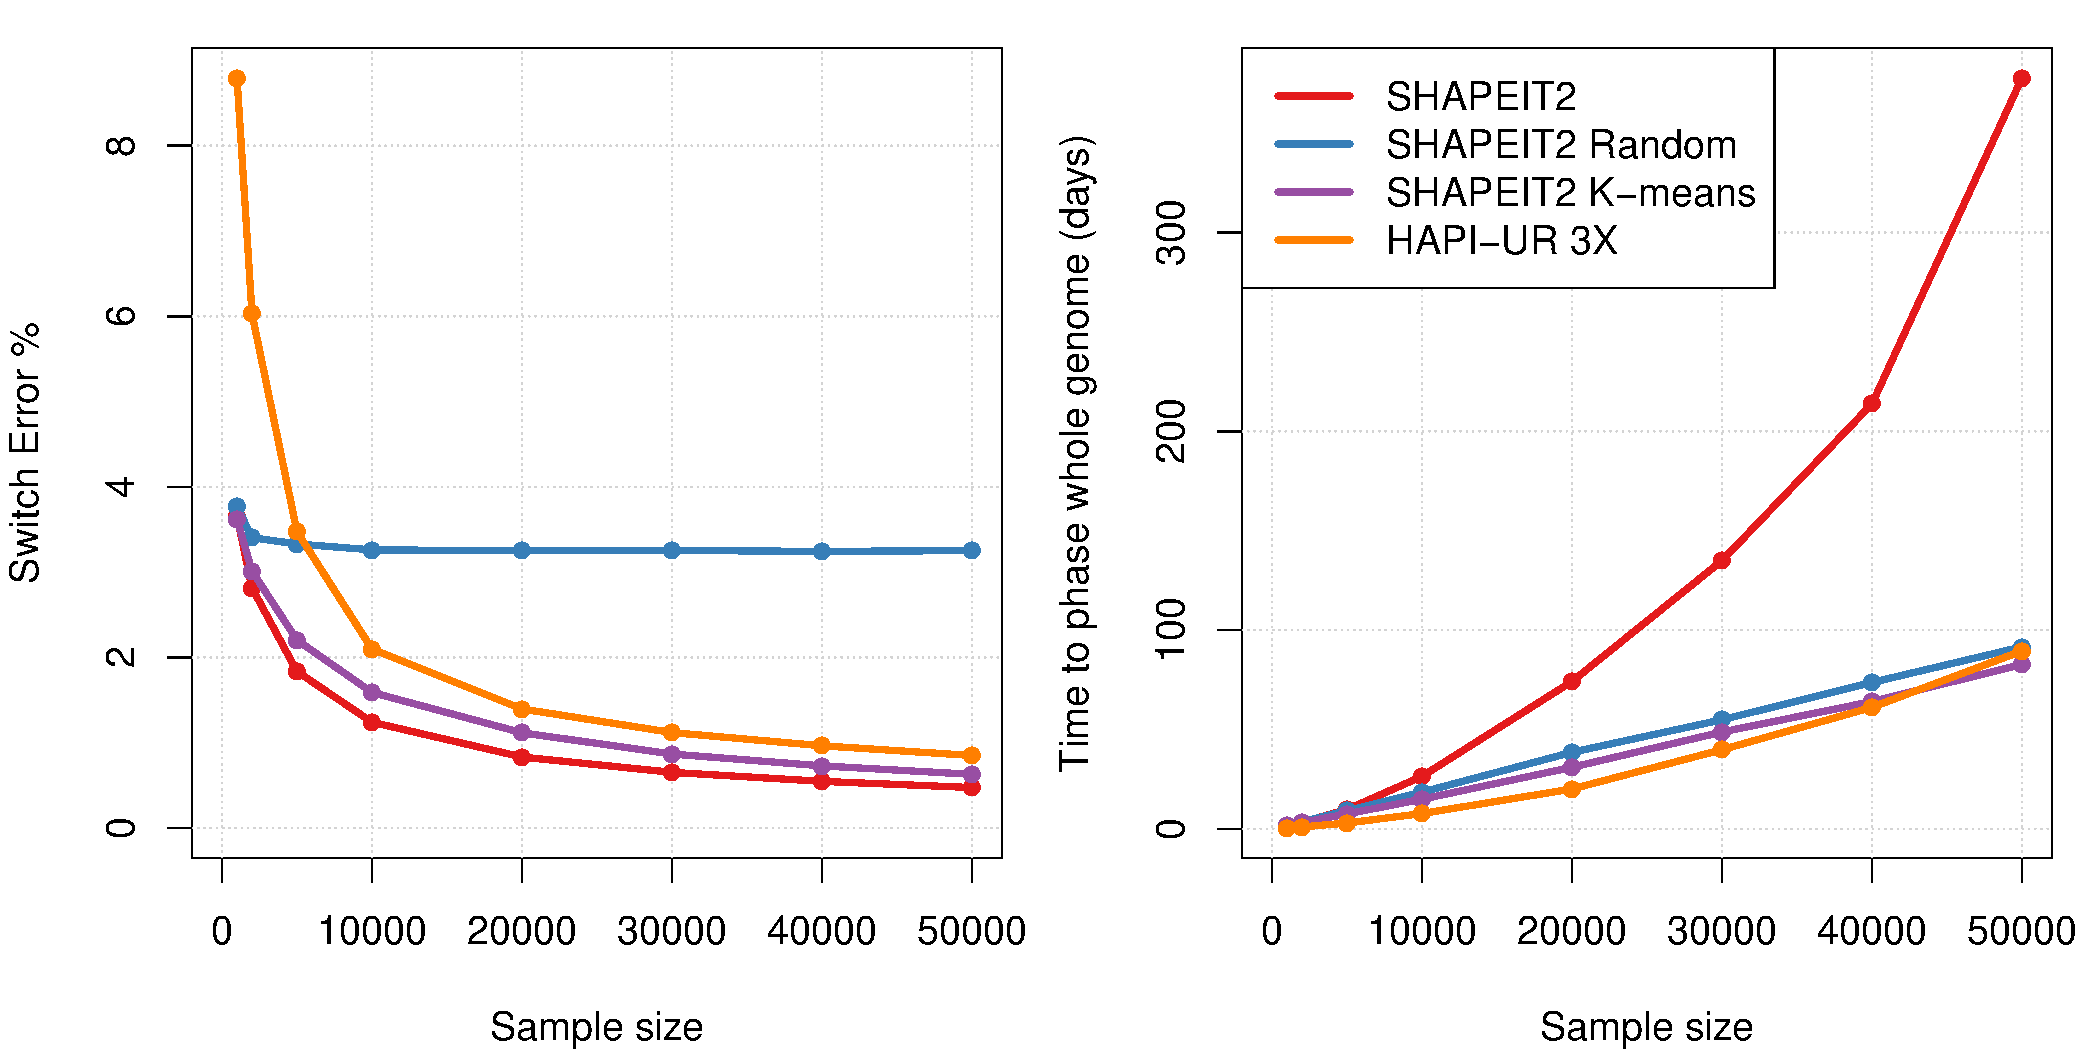
\includegraphics[width=\textwidth]{chap5figs/simulated}%\vspace{-20pt}
\caption[Accuracy and computation comparison for increasing sample sizes]{Accuracy and computational cost of different phasing routines on the WTCCC1+HapMap data (top) and the simulated Affymetrix 500 data (bottom). SHAPEIT2 is the standard implementation with a quadratic distance cost, `Random' does distance calculations on $M$ randomly chosen haplotypes, `K-means' compares all individuals within the same cluster resulting $\approx M$ comparisons per individual. We used $M=1000$ in all cases.  HAPI-UR3X  is three averaged runs of HAPI-UR. \textbf{Left:}~The switch error rate against sample size.  \textbf{Right:} The single CPU computation time in days for whole genome phasing (extrapolated from 10Mb) for each method on an Intel Xeon CPU E5-2690 (2.90GHz) CPU with 256GB of RAM. \label{chap5:switch}}
\end{figure}

\section{Discussion and Further Work}

The methods and results in this chapter are very preliminary, but are proof of the concept that SHAPEIT2 can be extended to larger samples. We saw that the K-means approach was quite effective at controlling computation whilst maintaining accuracy, resulting in a method that was more accurate and faster than HAPI-UR at 50,000 samples.  We hope to remove the modest loss of accuracy introduced with further modifications to the K-means partitioning technique. We also need to investigate how to correctly set the value of $M$.

The loss of accuracy when using K-means is likely due to the fact that a haplotype's nearest neighbour is not always in the same cluster, particularly for haplotypes that lie on the boundary between clusters.  A possible workaround to this problem would be to  allow observations to lie in multiple clusters, this is a similar idea to ``Canopy Clustering'' which is a popular method in data mining communities~\citep{mccallum2000efficient} for rapidly clustering large high-dimensional data sets. 

We have restricted our evaluations to using the Hamming distance metric, but there is no reason a more sophisticated distance measure could not be used.  One obvious measure would be to use the Euclidean distance between normalised alleles, $x_{il} = \frac{(H_{il} - p_l)}{\sqrt{p_l(1-p_l)}}$, where $p_l$ is the MAF at site $l$.  This would put greater weight on low frequency variants, which is sensible as they correlate with longer shared haplotype length.  This measure still ignores correlation between variants, we could also use the Mahalanobis distance measure which would involve modelling all SNPs in a window jointly with a multivariate normal distribution, providing a simple way of taking into LD into account.

This chapter touches on one small aspect of the issue that data is growing faster than computing power in the field of genetics.  This means that new approximate (but accurate) algorithms constantly need to be developed to allow tractable computation. This trend is abundantly clear in the field of haplotype phasing where the real benefit of new methods such as SHAPEIT2 and HAPI-UR has not only been improved accuracy, but substantially decreased computation time.



%next line adds the Bibliography to the contents page
\addcontentsline{toc}{chapter}{Bibliography}
%uncomment next line to change bibliography name to references
%\renewcommand{\bibname}{References}
\bibliography{thesis}
\bibliographystyle{authordate1}

\setcounter{table}{0}
\setcounter{figure}{0}
\renewcommand{\thefigure}{S\arabic{figure}}
\renewcommand{\thetable}{S\arabic{table}}

\appendix

\chapter{Evaluations to determine the final genotype calling model}\label{chiamantesup}
We have described our genotype calling method with a number of possible different variations on the model:
\begin{itemize}
  \item choice of distribution for array data - bivariate Gaussian or \st with $\upsilon=5$
  \item three possible prior distributions for the cluster centroids, $\mu$
  \item prior allele frequency distribution $\alpha$    
%  \item constant value for failure density $P(Y|Z^Y=1)$
\end{itemize}
We evaluated these options using chromosome 20 Omni2.5S data for 1,525 individuals (described in section~\ref{chap2:data}).  Concordance with the Affymetrix data (equation~\ref{concordance}) was evaluated for different parameterisations of the genotype calling method and was used (amongst other considerations) to determine the final choice of model that was used in our final comparisons with other genotype calling software in section~\ref{chap2:results:comparison}.  We assessed both the array-only scenario (1,525 individuals assayed on Illumina's chip) and the mixed array and sequence scenario (1094 of these individuals having 4X sequence data).

\section*{Choice of centroid priors and distribution} \label{centroidcompare}
\label{chap2:results:centroid}
When making genotype calls using only array data, the combination of the \st distribution and the third choice of priors (correlated centroids) performed the most accurately, albeit slightly, across the range of posterior probability thresholds (Figure~\ref{priorcompare}).  When the genotype calls were made with both array and sequence data, the \st distribution again performed better than the Gaussian, but the priors appear to have little effect on accuracy.  This makes intuitive sense as we have more data in this scenario, hence the priors are having limited effect on parameter estimates.  Given these results, we chose to use the mixture of \st distributions with the third choice of priors (Equation~\ref{model3}).

\begin{figure}[h]
  \begin{center} 
    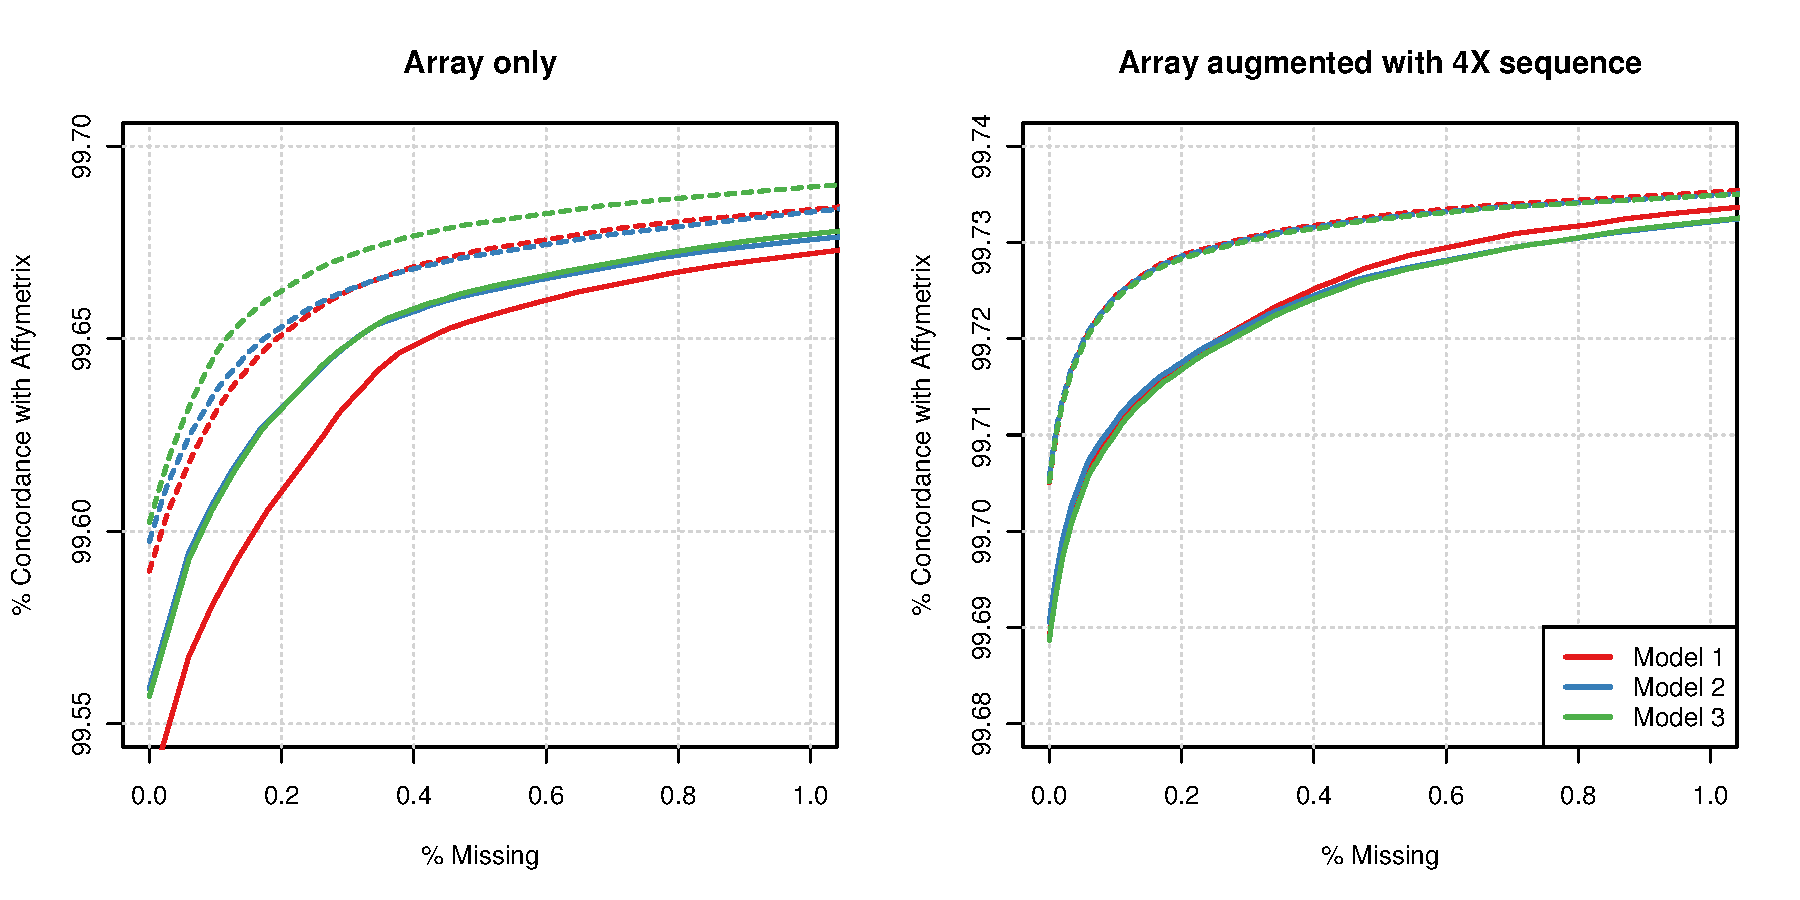
\includegraphics[width=\textwidth]{chap2figs/SupFig4}
    \caption[Evaluation of prior choices for centroids]{Comparison of our three possible choices of priors (coloured) and a mixture of Gaussian distributions (solid lines) versus a mixture of \st distributions with $\upsilon=5$ (dashed lines) for array only calls (left) and array data augmented with sequence data (right).  We can see that \st is consistently more accurate for both data sets and all choices of priors.  In the array only context, our third prior performs the most accurately (albeit slightly) when combined with the \st distribution.  Whilst when sequence data is included in the modelling, the choice of prior appears to have limited effect on accuracy.  Note the vertical scale varies between the plots, that is, the array augmented with sequence calls are $\approx$ 0.1\% more accurate than the array-only calls.\label{priorcompare}}
  \end{center} 
\end{figure}


\subsection*{Choice of allele and genotype frequency prior} \label{freqprior}
\label{chap2:results:exploratory:freq}
In section~\ref{chap2:priors} we described a flat Beta prior for the reference allele frequency. A well known result in population genetics~\citep{fu1995statistical} states that the distribution of alternate allele frequencies ($\alpha$ in our model) is inversely proportional to the frequency, that is $P(\alpha) \propto 1/\alpha$.  This result is not necessarily consistent with the loci frequencies present on a microarray.  We took an empirical approach to modelling the allele frequency spectrum of loci on the Omni2.5S chip. Loci information was downloaded from the 1000 Genomes FTP server \footnote{\url{ftp://ftp.1000genomes.ebi.ac.uk/vol1/ftp/release/20110521/ALL.wgs.phase1_release_v3.20101123.snps_indels_sv.sites.vcf.gz}}, global allele frequencies for the Omni 2.5S positions were then extracted from this file and we estimated parameters for the Beta(a,b) distribution using maximum likelihood ($\hat{a}=0.363,\hat{b}=1.254$).  The fit of this distribution appears very reasonable (Figure~\ref{AFS_betafit}).


\begin{figure}[h]
\begin{center} 
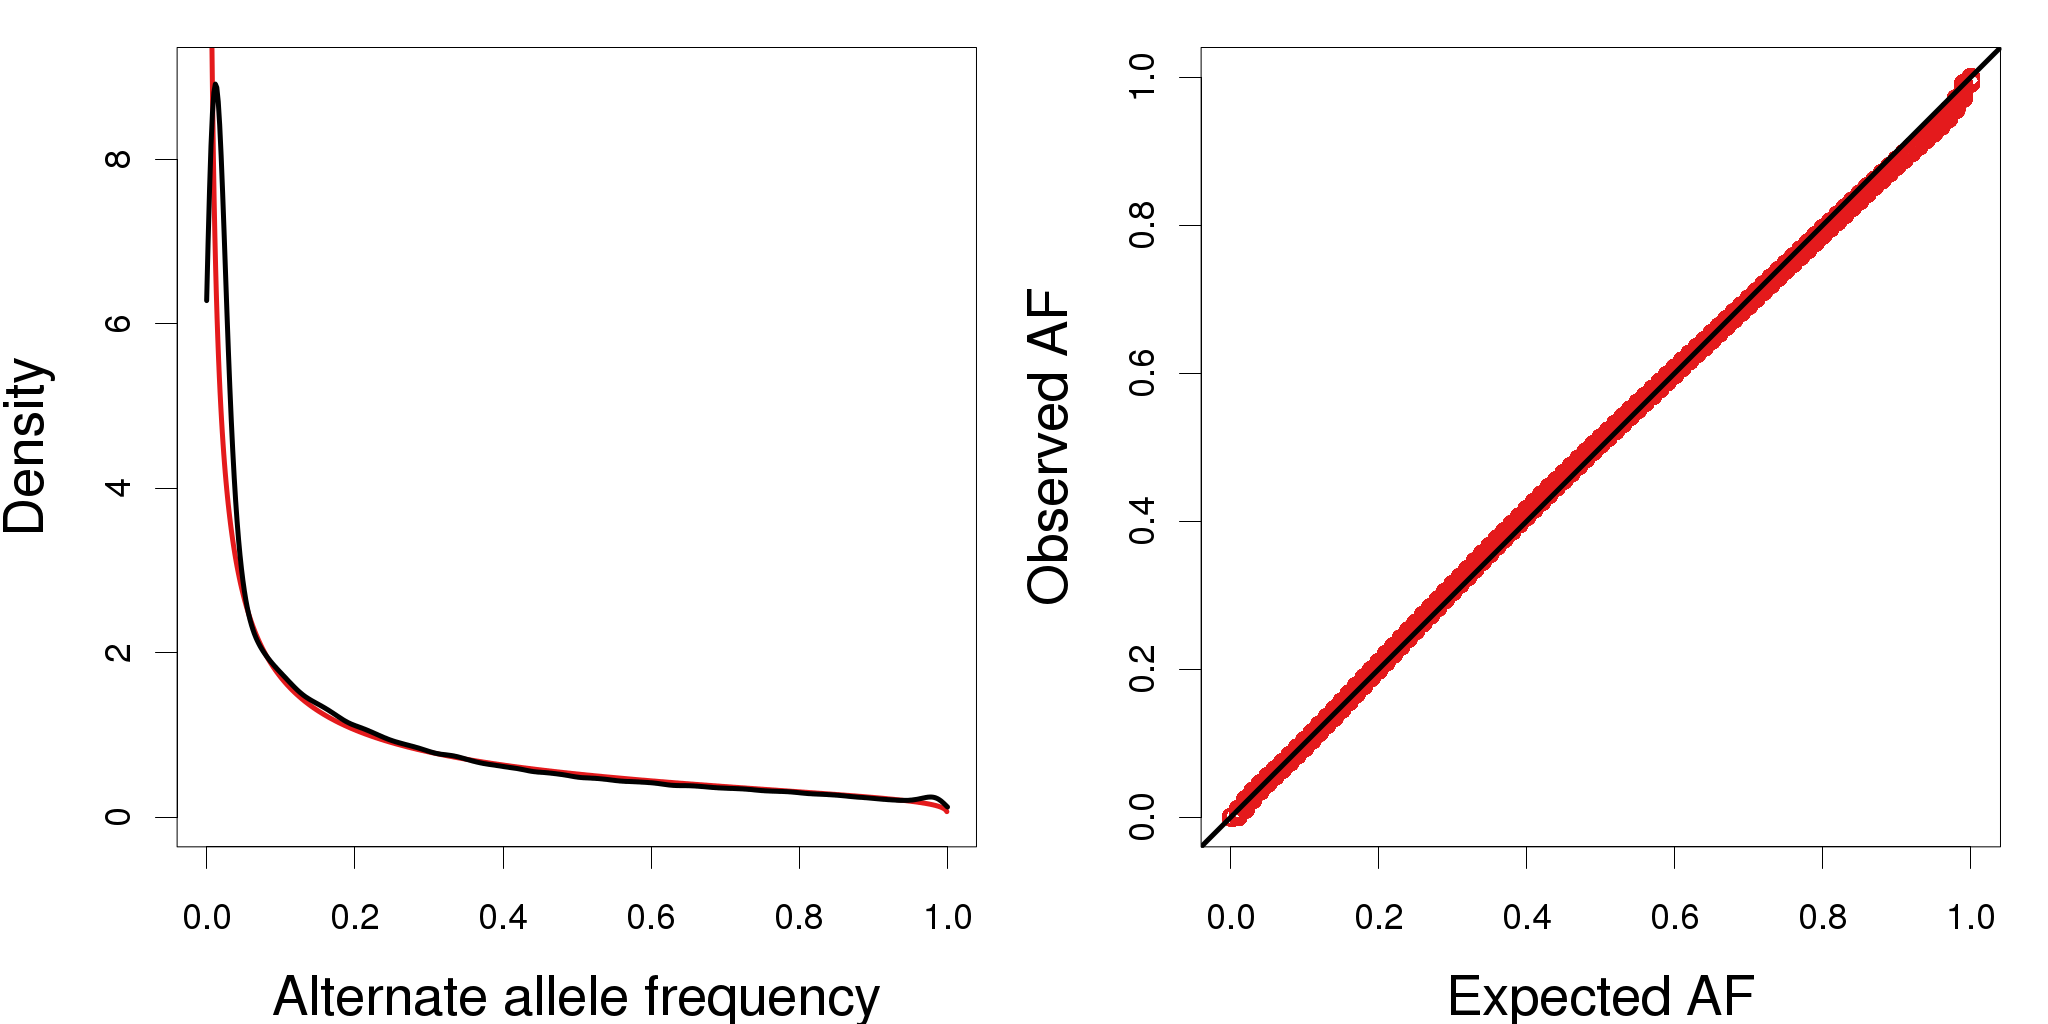
\includegraphics[width=\textwidth]{chap2figs/SupFig2}
\caption[Allele frequency spectrum on Omni2.5S chip]{\textbf{Left:} Kernel smoothed density estimate of the alternate allele frequency spectrum on the Omni2.5S chip (black) and a Beta distribution fitted to these frequencies.  \textbf{Right:} Q-Q plot of the empirical quantiles of the frequencies against theoretical quantiles of the Beta distribution.
\label{AFS_betafit}}
\end{center} 
\end{figure}
\clearpage
We used a Dirichlet prior for the genotype frequencies that allows some deviation from Hardy-Weinberg Equilibrium. After one generation of random breeding a population will be in HWE.  However, in a case-control GWAS the cases may deviate from HWE due to biased sampling of causative alleles so allowing some departure from HWE may be desirable.

To investigate the effect of our choice of priors on accuracy we called genotypes using only array data on the 1,525 samples for all loci on chromosome 20 using five different priors. 

\begin{enumerate}\label{freqpriorlist}
\item a flat Beta prior for reference allele frequency with departure from HWE allowed ($\delta=10$)
\item a flat Beta prior for reference allele frequency with \emph{no departure} from HWE allowed
\item the estimated Beta distribution for reference allele frequencies with departure from HWE allowed ($\delta=10$)
\item the estimated Beta distribution for reference allele  \emph{no departure} from HWE allowed
\item a flat Dirichlet prior for genotype frequencies $\lambda \sim \textrm{Dirichlet}(1,1,1)$
\end{enumerate}

We found the forced HWE priors to be slightly more accurate than our Dirichlet prior (with some HWE penalty) and than the flat Dirichlet prior with no HWE deviation penalty (Figure~\ref{freq_prior_comparison}).  However, in case-control GWAS allowing deviation from HWE may be desirable.  Whilst the Beta prior estimated from population data was (marginally) more accurate we left the Beta prior as flat since this accuracy is conceivably due to over fitting.  In any case, the choice of priors for $\alpha$ and $\lambda$ clearly have a limited effect on accuracy. We leave $\delta$ as a tuneable parameter in our software (with $\delta=10$ as the default value). 

\begin{SCfigure}[1][h]
\centering
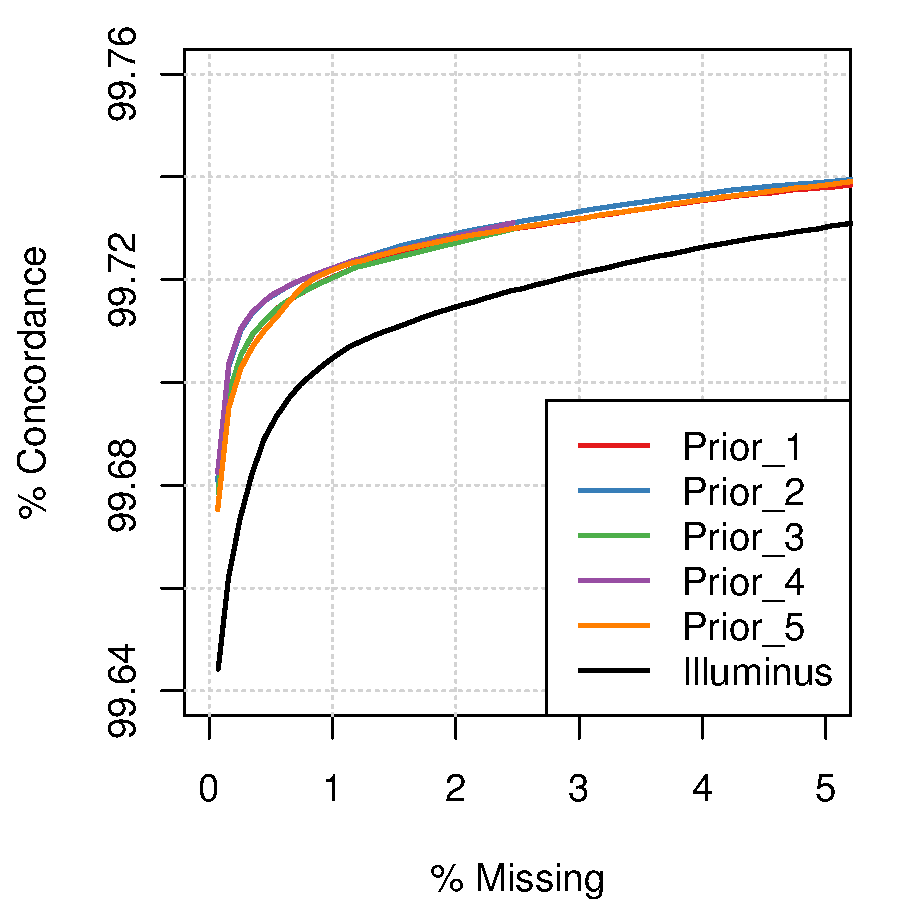
\includegraphics[width=.5\textwidth]{chap2figs/SupFig3}
\caption[Evaluation of prior choices for allele frequency]{Concordance against missing data rate for five different priors described in~\ref{freqpriorlist}; \textbf{1.} a flat Beta prior for reference allele frequency with departure from HWE allowed ($\delta=10$ in Eq. 2)
\textbf{2.} a flat Beta prior for reference allele frequency with \emph{no departure} from HWE allowed
\textbf{3.} the estimated Beta distribution for reference allele frequencies with departure from HWE allowed ($\delta=10$ in Eq. 2)
\textbf{4.} the estimated Beta distribution for reference allele  \emph{no departure} from HWE allowed
\textbf{5.} a flat Dirichlet prior for genotype frequencies $\lambda \sim \textrm{Dirichlet}(1,1,1)$
\label{freq_prior_comparison}}
\end{SCfigure}


%% \subsubsection{Choice of sequence failure density} 
%% \label{chap2:results:fail_dens}
%% There was no obvious way to choose a value for $P(Y_i|Z_{Y_i}=1)=h_Y(y_i)$ and a constant value is likely to be overly simplistic.  Realistically it should be some function of typical sequencing QC measures such as coverage, mapping quality and base quality. However this was beyond the scope of our method which aims to leverage sequence data in a simple manner to improve the accuracy of genotype microarry data. Hence we undertook a simple empirical experiment, trying a range of values for $h_Y(y_i)$ and calculating concordance (Figure~\ref{fail_dens}). We found that actually setting $h_Y(y_i)=0.01$ leads to extremely marginally better results than $h_Y(y_i)=0.0$ and as $h_Y(y_i)$ increases the accuracy tends to what we see when no sequencing data is used (not surprisingly).  This result may lead us to consider removing the failure indicator for sequencing data altogether but this is specious reasoning.  Due to false variant calls in the Pilot sequencin of the 1000 Genomes Project, roughly 8\% of sites on the Omni2.5S chip are monomorphic (supplementary table~\ref{chap2:locisummary} improvements in sequencing technology and bioinformatics also mean these sites are correctly called as monomorphic in sequencing data although some errors remain.  Loci that are present on both the Affymetic and Omni chips are more likely to be genuine SNPs and well ascertained by sequencing pipelines.  When we look at the the Q-Q plots (for \emph{all} Omni SNPs) for divergence from Hardy-Weinberg Equilibrium Figure~\ref{fail_dens} (right) for differing values of $h_Y(y_i)$ we can see for $h_Y(y_i)=0$

%% .Section~\ref{chap2:results:errors} also shows some futher utility of the sequence failure indicator variable.

%% \begin{figure}[ht!]
%% \begin{center} 
%%   \includegraphics[width=.5\textwidth]{chap2figs/SupFig12}
%% \caption{Concordance with Axiom against missing data rate for varying values of $P(Y|Z^Y=1)$ on chromsome 20.  Calls were made using 1525 inviduals assayed on the Omni2.5S data, a subset of 1094 individuals were also sequenced at 4X.  Calls from Chiamante using only array data are included for scale. \label{fail_dens}}
%% \end{center} 
%% \end{figure}


\chapter{Supplemental Tables}
\begin{table}[ht]\footnotesize
\begin{center}
\begin{tabular}{ |r|rrrrrr|}
\hline
& Illumina  & Affymetrix & 4X &  Omni2.5S & Omni2.5S & Omni2.5S/\\
Population &  Omni2.5S & Axiom & sequence & 4Xsequence & Axiom &Axiom/ \\
& & & & &&Sequence \\
\hline

ASW & 96 & 90 & 61 & 61 & 88 & 53 \\ 
CEU & 104 & 180 & 87 & 87 & 101 & 84 \\ 
CHB & 100 & 90 & 97 & 97 & 86 & 85 \\ 
CHD & 0 & 90 & 0 & 0 & 0 & 0 \\ 
CHS & 150 & 0 & 100 & 100 & 0 & 0 \\ 
CLM & 107 & 0 & 60 & 60 & 0 & 0 \\ 
FIN & 100 & 0 & 93 & 93 & 0 & 0 \\ 
GBR & 96 & 0 & 89 & 89 & 0 & 0 \\ 
GIH & 0 & 90 & 0 & 0 & 0 & 0 \\ 
IBS & 69 & 0 & 14 & 14 & 0 & 0 \\ 
JPT & 100 & 91 & 89 & 89 & 91 & 80 \\ 
LWK & 100 & 90 & 97 & 97 & 90 & 87 \\ 
MKK & 31 & 180 & 0 & 0 & 31 & 0 \\ 
MXL & 100 & 90 & 66 & 66 & 90 & 56 \\ 
PUR & 111 & 0 & 55 & 55 & 0 & 0 \\ 
TSI & 100 & 90 & 98 & 98 & 90 & 90 \\ 
YRI & 161 & 180 & 88 & 88 & 161 & 88 \\ 
\hline
ALL & 1525 & 1261 & 1094 & 1094 & 828 & 623 \\ 
\hline

\end{tabular}
\caption[Summary of 1000 Genomes data used in genotype calling]{Summary of the samples that have been assayed on the three technologies as well as the intersections of these technologies.\label{sampleinfo}}
\label{chap2:sampleinfo}
\end{center}
\end{table}

\begin{table}
\begin{center}
\begin{tabular}{|l|r|rr|rr|rr|}
\hline
\multicolumn{8}{|c|}{Chiamante (no sequence)}\\
\hline
&&\multicolumn{2}{c}{828}&\multicolumn{2}{|c}{623}&\multicolumn{2}{|c|}{205}\\
\hline
Filter & SCR & GCR & Conc & GCR & Conc & GCR & Conc \\ 
\hline
None & 100.000 & 99.824 & 99.696 & 99.838 & 99.695 & 99.788 & 99.696 \\ 
GCR & 99.765 & 99.646 & 99.698 & 99.661 & 99.698 & 99.607 & 99.698 \\ 
HWE & 99.941 & 99.766 & 99.708 & 99.781 & 99.708 & 99.730 & 99.707 \\ 
PP & 100.000 & 99.744 & 99.715 & 99.767 & 99.714 & 99.686 & 99.717 \\ 
\hline
GCR+HWE & 99.710 & 99.590 & 99.709 & 99.605 & 99.710 & 99.552 & 99.709 \\ 
PP+GCR & 99.694 & 99.520 & 99.722 & 99.545 & 99.722 & 99.457 & 99.724 \\ 
PP+HWE & 99.940 & 99.696 & 99.722 & 99.719 & 99.722 & 99.636 & 99.724 \\ 
\hline
All & 99.659 & 99.486 & 99.726 & 99.511 & 99.726 & 99.423 & 99.728 \\ 
\hline
\end{tabular}
% \caption{SCR, GCR and concordance with Axiom data for a call set produced using Chiamante with Omni2.5S data on 1525 1000 Genomes individuals (no sequence data was used in this analysis). 
% Metrics were calculated on 828 inviduals with Axiom data available, and then on the same 828 individuals split into two groups; 623 who had 4X sequence data available and 205 who had no sequence data available.
% }
% \end{center}
% \end{table}

% \begin{table}[ht]
% \begin{center}
~\\
~\\
\begin{tabular}{|l|r|rr|rr|rr|}
\hline
\multicolumn{8}{|c|}{Chiamante + Sequence}\\
\hline
&&\multicolumn{2}{c}{828}&\multicolumn{2}{|c}{623}&\multicolumn{2}{|c|}{205}\\
\hline
Filter & SCR & GCR & Conc & GCR & Conc & GCR & Conc \\ 
\hline
None & 100.000 & 99.986 & 99.721 & 100.000 & 99.723 & 99.950 & 99.714 \\ 
GCR & 99.985 & 99.974 & 99.722 & 99.985 & 99.724 & 99.946 & 99.715 \\ 
HWE & 99.984 & 99.970 & 99.723 & 99.984 & 99.725 & 99.934 & 99.716 \\ 
PP & 100.000 & 99.940 & 99.733 & 99.968 & 99.734 & 99.869 & 99.729 \\ 
\hline
GCR+HWE & 99.969 & 99.958 & 99.723 & 99.969 & 99.726 & 99.930 & 99.717 \\ 
PP+GCR & 99.966 & 99.914 & 99.734 & 99.938 & 99.736 & 99.853 & 99.731 \\ 
PP+HWE & 99.986 & 99.927 & 99.734 & 99.955 & 99.735 & 99.856 & 99.730 \\ 
\hline
All & 99.954 & 99.903 & 99.736 & 99.927 & 99.737 & 99.841 & 99.732 \\ 
\hline
\end{tabular}
\caption[Breakdown of genotype calling performing for
sequenced/non-sequenced samples]{\textbf{Top:} SCR, GCR and concordance with Axiom data for a call set produced using Chiamante with Omni2.5S data on 1525 1000 Genomes individuals (no sequence data was used in this analysis).  Metrics were calculated on 828 individuals with Axiom data available, and then on the same 828 individuals split into two groups; 623 who had 4X sequence data available and 205 who had no sequence data available. \textbf{Bottom:} The same metrics for a call set produced with the same array data, but augmented with sequence information from a subset of 1094 individuals. We can see that there is an improvement in call rate and accuracy not only for the 623 individuals with sequence data, but also for the 205 individuals without sequence data.\label{chap2:results:splitchi}}
\end{center}
\end{table}


%% \begin{table}[ht]
%% \begin{center}
%% \begin{tabular}{rrrrrr}
%%   \hline
%%  Chromosome & Omni2.5S & BCM GLs & Axiom & Omni\_Axiom & All \\ 
%%   \hline
%%    1 & 191197 & 174203 & 441079 & 95930 & 95381 \\ 
%%  2 & 200037 & 183761 & 517849 & 108980 & 108392 \\ 
%%  3 & 167887 & 154328 & 459423 & 95341 & 94843 \\ 
%%  4 & 157357 & 144584 & 456698 & 89225 & 88700 \\ 
%%  5 & 149731 & 137635 & 412448 & 83865 & 83356 \\ 
%%  6 & 150265 & 137805 & 399701 & 84366 & 83846 \\ 
%%  7 & 133887 & 122945 & 335660 & 70574 & 70204 \\ 
%%  8 & 129541 & 119866 & 358241 & 72427 & 72042 \\ 
%%  9 & 107141 & 99329 & 258727 & 56843 & 56544 \\ 
%%  10 & 123548 & 113569 & 287587 & 63239 & 62880 \\ 
%%  11 & 120676 & 110840 & 281381 & 61709 & 61354 \\ 
%%  12 & 116228 & 106306 & 278340 & 61740 & 61364 \\ 
%%  13 & 85737 & 78986 & 232032 & 48592 & 48297 \\ 
%%  14 & 79307 & 73150 & 192567 & 42439 & 42214 \\ 
%%  15 & 74520 & 68661 & 166476 & 38813 & 38591 \\ 
%%  16 & 80838 & 74748 & 153351 & 35699 & 35526 \\ 
%%  17 & 70478 & 64676 & 111189 & 26903 & 26780 \\ 
%%  18 & 70476 & 65391 & 186324 & 39786 & 39550 \\ 
%%  19 & 52612 & 48034 & 56590 & 15256 & 15177 \\ 
%%  20 & 59114 & 55034 & 119865 & 28131 & 28029 \\ 
%%  21 & 33403 & 30738 & 79193 & 16809 & 16692 \\ 
%%  22 & 36064 & 33449 & 42188 & 11640 & 11504 \\ 
%% \hline
%%   All & 2390044 & 2198038 & 5826909 & 1248307 & 1241266 \\ 
%%    \hline
%% \end{tabular}
%% \caption{Number of autosomal SNPs present on the Omni2.5S chip, intersecting with BCM sequence likelihoods, Axiom and the intersection of all three pieces of data. Around 192006 ($\approx$ 8\%) of the chip positions were missing from the 1000G sequence genotype likelihoods but of these missing locations, only 7041 ($ \approx$ 0.3\%) were on the Axiom chip.}
%% \label{chap2:locisummary}
%% \end{center}
%% \end{table}

\chapter{Data sets}


\section*{Isolates data}
INGI-FVG and INGI-CARL: We would like to thank the people of the Friuli Venezia Giulia Region and of Carlantino for the everlasting support.

ORCADES: DNA extractions were performed at the Wellcome Trust Clinical Research Facility in Edinburgh. We would like to acknowledge the invaluable contributions of Lorraine Anderson and the research nurses in Orkney, the administrative team in Edinburgh and the people of Orkney.

Val Borbera: We thank the inhabitants of the Val Borbera for participating in the study, and the local administrations and the ASL-Novi Ligure for support, Fiammetta Vigan\`{o} for technical support and Professor Clara Camaschella for help with clinical data collection. 

CROATIA-Split, CROATIA-Vis, CROATIA-Korcula: We thank the inhabitants of the Split, Vis and Korcula for participating in the study.


\section*{WTCCC data}
This work makes use of data generated by the Wellcome Trust Case Control Consortium. A full list of the investigators who contributed to the generation of the data is available at \url{www.wtccc.org.uk}. Funding for the project was provided by the Wellcome Trust under awards 076113 and 085475.


\end{document}

